\documentclass[11pt]{report}
\usepackage[french,english]{babel}
\selectlanguage{french}
\usepackage{graphicx}
\usepackage[utf8]{inputenc} 
\usepackage[total={6.5in,8.75in}, top=0.6in, bottom=0.4in, left=1.0in, includefoot]{geometry}
\setlength{\parindent}{0cm}
\usepackage{caption}

\usepackage[T1]{fontenc}
\usepackage{lmodern}
\usepackage{amsmath}
\usepackage{multicol}
\usepackage{array}
\usepackage{amssymb}
\usepackage{mathrsfs}
\usepackage{lscape}
\usepackage{url}
\usepackage{textcomp}
%\usepackage{microtype}
%\DisableLigatures{}
\newcommand{\imgHeightSmall}{5cm}
\newcommand{\imgHeightMedium}{7.5cm}
\newcommand{\imgHeightBig}{12.5cm}

\begin{document}
	%\title{Serious Game 3D temps réel pour la réhabilitation  \\ \vspace{2 mm}  Rapport}
	%\author{Nicolas Wenk}
	%\date{\today}
	%\maketitle
	
	\begin{titlepage}
	
	\hspace{-0.6in}{
		\begin{picture}(0,0)
		{
				
\includegraphics{img/Title_MSE.png}
		}
		\end{picture}
	}
	
	\begin{flushright}
	\begin{picture}(144,0)
	{
			
\includegraphics[width=50mm]{img/Title_Hesso.png}
	}
	\end{picture}
	\end{flushright}
	
	\begin{flushleft}
		\hspace{-0.6in}{
			\parbox{10cm}{
				\small
				Master of Science HES-SO in Engineering\\
				Av. de Provence 6\\
				CH-1007 Lausanne\\
			}
		}
	\end{flushleft}
	
	\begin{center}
	\large
	\textsc{\MakeUppercase {}}\\
	\end{center}
	
	
	\begin{flushright}
		\vspace*{1cm}
		\huge
		Master of Science HES-SO in Engineering\\
		
		\vspace{0.5cm}
		\large
		Orientation: Technologies de l'information et de la communication (TIC)\\
		\vspace*{1cm}
		\huge
		\MakeUppercase {Serious Game 3D temps réel}
		
		\MakeUppercase{pour la réhabilitation}\\
		
		\normalsize
		\vspace{4.5cm}
		Fait par\\
		\huge
		Nicolas Wenk\\
		
		\vspace{1cm}
		\normalsize
		Sous la direction de\\
		Prof. Nabil Ouerhani\\
		Dans le groupe de compétence Imagerie de la HE-Arc\\
		
		\vspace{1cm}
		Expert externe: Quentin Silvestre
		
		\vspace{1cm}
		Lieu, HES-SO//Master, 2016\\
		
	\end{flushright}

\end{titlepage}

	\newpage
	%\newgeometry{left=30mm,right=30mm, top=50mm, bottom=20mm}
	\begin{titlepage}
	\begin{flushleft}
			%TODO: Voir comment et si intégrer STG
			Accepté par la HES-SO//Master (Suisse, Lausanne) sur proposition de\\
			
			\vspace{0.5cm}
			Prof. Nabil Ouerhani, conseiller de travail de Master\\
			Quentin Silvestre, Expert principal\\
			\vspace{1cm}
			St-Imier, le 05.02.2016\\
			\vspace{3cm}
			\begin{multicols}{2}
			Prof. Nabil Ouerhani\\
			Conseiller\\
			
			\columnbreak
			
			Prof. Moghaddam Bützberger Fariba\\
			Responsable de la filière \textit{Master of Science in Engineering}.\\
		\end{multicols}
	\end{flushleft}
\end{titlepage}
	\newpage

	\pagenumbering{roman}
	
	\renewcommand\labelitemi{\textbullet}
	\renewcommand\labelitemii{\textbullet}
	\renewcommand\labelitemiii{\textbullet}

	\chapter*{Abstract}
		\selectlanguage{english}

The goal of this work is the creation of a neurorehabilitation serious game (SG) for the lower limbs using the rehabilitation device called Lambda Health System (LHS). Users are suffering of paresis in those limbs and have to learn to walk again. Those people may also suffer of cognitive troubles like hemineglect which is an important concept to keep in mind for the realization of the SG.
\\

The SG main goal is to add ludic aspects to physiotherapist's exercise which consists of the repetitive walking movements. The three other important aspects of this SG: high immersion; environment able to be impoverished according to the patient's cognitive abilities; visualization of the walking movement. The later aims to enabling mirror neurons and to enhancing the rehabilitation process. 
\\
 
The developped SG is an exploration game where the user, guided on a path, has to walk to be able to progress with the trigger to find civilisation's vestiges. The distribution of their left/right placement is given by the therapist.
\\

The look is retrieved with an Head Mounted Display. Such device is well known to be one of the best nowadays for visual immersion. Furthermore, the hearing sense is stimulated by footsteps noises, background sound, music and UI sounds. The only sense awaited but not actually present is the touch. He is supposed to be stimulated by haptic rendering in the LHS. Relating to the impoverishment, nine factors are implemented. They change the geometries, the light effects, the animations, the sounds, the colors and the density of the world. For the movement representation, the game is in first person and the avatar's legs are animated as the patient's ones. Another virtual character is ahead of the user all along the path doing a walking animation.
\\

Due to current official testings in the "Centre Hospitalier Universitaire Vaudois" (CHUV), the integration of the SG in the LHS system is prepared but not tested yet. The walking movement is simulated by a keyboard key. However, a meeting with a medical doctor was scheduled to show the actual SG. Encouraging feedback was received regarding its utility even for patients suffering of cognitive troubles, without a movement therapy.
\\

Keywords: serious game, lower limb neurorehabilitation, virtual reality, virtual world, immersion, cognitive impoverishment, hemineglect, multimodal.

\selectlanguage{french}	
	
	\chapter*{Résumé}
		Ce travail a pour but la création d'un \textit{serious game} (SG) pour la neuroréhabilitation des membres inférieurs utilisant le périphérique de réhabilitation \textit{Lambda Health System} (LHS). Les utilisateurs sont des personnes souffrant de parésies de ces mêmes membres, ils doivent réapprendre un mouvement de marche. Ces personnes souffrent également fréquemment de troubles cognitifs, dont notamment l'héminégligence, à prendre en compte pour le SG.
\\

Le but principal du SG est donc d'ajouter un aspect ludique à un exercice de physiothérapie consistant à la répétition d'un mouvement de marche. Ce SG a également trois autres aspects importants: une haute immersion; un environnement pouvant être appauvrit pour s'adapter aux troubles cognitifs du patient; une visualisation du mouvement de marche. Ce dernier a pour but d'activer les neurones miroirs et ainsi d'améliorer le processus de réhabilitation.
\\
 
Le SG implémenté consiste en l'exploration de planètes à la recherche de traces d'une civilisation disparue. Ceci sur des parcours guidés où le patient doit avancer en marchant. La répartition gauche/droite des vestiges le long du chemin est définie par le thérapeute.
\\

La recherche de ces traces se fait à l'aide d'un casque de réalité virtuelle. Ce périphérique est connu pour être un des meilleurs actuel pour une immersion visuelle. Le sens de l'ouïe est stimulé à l'aide de bruits de pas, de sons d'ambiance, de musiques et de sons d'interface. Le toucher est également visé à l'aide du retour haptique du LHS. Il n'est cependant pas présent actuellement. Pour l'appauvrissement, neuf facteurs ont été réalisés, influant sur la géométrie, les effets de lumière, les animations, les sons, les couleurs et la densité des éléments. Concernant la représentation du mouvement, le joueur joue à la première personne et les jambes de son avatar sont articulées pour correspondre aux mouvements des siennes. Un autre personnage virtuel est placé devant le joueur durant tout le parcours et possède une animation de marche.
\\

Dû à des tests officiels réalisés au Centre Hospitalier Universitaire Vaudois (CHUV), l'intégration au LHS, bien que préparée, n'a pas pu être testée. Le mouvement est, par conséquent, simulé au clavier. Une rencontre avec un médecin a cependant permis d'obtenir des retours encourageants sur le SG actuel, même en dehors d'une réhabilitation de marche pour des personnes souffrant de troubles cognitifs.
\\

Mots clés: \textit{serious game}, neuroréhabilitation des membres inférieurs, réalité virtuelle, monde virtuel, immersion, appauvrissement cognitif, héminégligence, multimodal.
		
		
	\chapter*{Remerciements}
		Tout d'abord, je tiens à remercier le Prof. Dr. Stéphane Gobron pour ses conseils et son encadrement tout au long de ce travail.
Je remercie Messieurs Aurélien Fauquex et Yannick Charrotton de "Lambda Health System S.A." pour les différentes séances réalisées durant ce projet ainsi que pour le travail fournit durant le projet précédent, notamment au niveau de la communication des SGs au LHS qui a été réutilisée.
Concernant également la communication mais aussi l'intégration du HMD, je tiens à remercier Monsieur Nicolas Zannini pour avoir effectué ces tâches durant son travail de Master ainsi que pour sa disponibilité durant ce projet.
\\

Je tiens également à remercier Monsieur Kevin Laipe ayant rejoint le groupe de compétences imagerie de la HE-Arc en tant que stagiaire durant ce travail. Son aide s'est avérée précieuse pour la création de niveaux supplémentaires et également pour la création de nouvelles fonctionnalités. Je le remercie aussi pour le temps passé à tester les fonctionnalités du SG, ce qui a permis d'identifier à temps certains \textit{bugs} et de les corriger.
\\

Je tiens à remercier le Prof. Dr. Michel Lauria de la HES-SO de Genève d'avoir participé à la définition et à la sélection des objectifs ainsi qu'à l'élaboration du concept du SG.
Je tiens à remercier le Dr. Rolf Frischnecht, médecin cadre du CHUV et membre de l'équipe LHS pour s'être déplacé à St-Imier et avoir testé le SG. Les retours recueillis, issus des nombreuses minutes passées en immersion dans la réalité virtuelle, sont encourageants et permettent d'envisager la suite de ce travail d'après un avis du domaine médical.
\\

Je remercie également Madame Améthyste Molin pour la relecture de ce document et les corrections pertinentes apportées.
\\

Je remercie d’avance Monsieur Quentin Silvestre, l’expert de mon travail de Master, pour le temps qu’il consacrera à la lecture de ce mémoire et pour sa future participation à ma défense de Master.
	
	\tableofcontents
	
	\chapter{Introduction}
		\pagenumbering{arabic}
		Ce projet est réalisé en tant que travail de Master pour conclure la formation "Master of Science in Engineering" en "Technologies de l'Information et de la Communication" proposée par la HES-SO. Il consiste à la conception et au développement d'un \textit{serious game} (SG) de marche avec une grande immersion pour la réhabilitation des jambes chez des patients souffrant de traumatismes neurologiques. Ce travail est contenu et est réalisé en amont d'un projet de recherche et développement (projet R\&D) dont il partage une partie des objectifs. Il fait également suite à plusieurs projets, dont le plus récent est "\textit{Serious Games for Rehabilitation}" (SG4R). Ce dernier fut réalisé en collaboration entre la HE-Arc, l'hepia, et la HEIG-VD ainsi qu'en étroite collaboration avec le CHUV et la Haute Ecole de Santé de Lausanne (HESAV). Il a donné lieu à une plateforme de prototypes de SGs fonctionnels, qui ont fait l'objet d'un user test auprès de spécialistes de la santé au CHUV.
\\

Un SG est un jeu où l'amusement est utilisé pour une intention sérieuse étant ici la réhabilitation des jambes. Le but est que le patient (premier utilisateur) fasse sa réhabilitation tout en s'amusant. Il faut également veiller à éviter d'ajouter de la complexité pour le thérapeute (second utilisateur) qui est habitué à travailler avec des exercices et non des jeux. Les patients sont des personnes devant réapprendre un mouvement de marche. La réhabilitation ciblée n'est pas musculaire mais neurologique (neuroréhabilitation) et se base sur la capacité de notre cerveau à refaire de nouvelles connexions (neuroplasticité). Son objectif est de récréer ou de remodeler les connexions inter-neuronales perdues à la suite d’un accident. Les exercices de rééducation consistent à réaliser des mouvements répétitifs pour que le cerveau réapprenne à les faire. %TODO Trouver une description plus précise des utilisateurs
\\

Les projets antérieurs ont également permis l'établissement d'une communication et le début d'une intégration entre les jeux réalisés à l'aide du logiciel \textit{Unity} et le dispositif de réhabilitation "Lambda". Le dispositif est souvent appelé "LHS" -- de "Lambda Health System" -- qui est en réalité le nom de la start-up le fabriquant et également le mandant de ce projet. Ce système permet de répondre aux besoins des thérapeutes et d'offrir des thérapies variées en un seul dispositif paramétrable. Il consiste en un robot, une interface homme-machine (IHM) ainsi qu'une couche software.
Le robot est motorisé et permet de mobiliser les jambes dans le plan sagittal mais il possède également des capteurs pour détecter la force appliquée par le patient. Grâce à la couche software exécutée dans un environnement temps réel ainsi qu'à de nombreuses modélisations de mouvements, le système est capable de détecter l'intention de mouvement du patient et de l'accompagner dans une trajectoire définie. Finalement, l'interface homme machine permet au personnel médical d'entrer les données du patient ainsi que de lui choisir et paramétrer des séances de réhabilitation composées d'exercices paramétrables.
\\

Pour ce projet, ce robot est utilisé et considéré comme périphérique principal pour le SG (ce qui était déjà le cas dans le projet antérieur). Le SG peut avoir accès aux informations physiques du patient ainsi que les valeurs des capteurs ou d'autres données traitées par la couche software (tel que la position des pieds dans un repère donné). Du point de vue du thérapeute ou de l'IHM, le SG doit être considéré comme un nouvel exercice.
\\

D'autres facteurs tels que les neurones miroirs peuvent également influer sur la qualité de la réhabilitation. Ces dernières peuvent être sollicitées notamment par le placement du patient dans une réalité virtuelle où une représentation du mouvement est présente. Cet effet est renforcé avec l'immersion du patient. Trois sens sont visés pour l'immersion. La vue: à l'aide d'un casque de réalité virtuelle; L'ouïe: à l'aide d'un casque sonore, de sons 3D et d'une musique d'ambiance; Le toucher: via le retour haptique du robot.
\\

D'autres périphériques additionnels sont envisageables, tels que, par exemple, une manette de jeu, une souris, un clavier, etc. Ces derniers doivent cependant éviter de détériorer la qualité de l'interaction avec le robot. Les interactions additionnelles peuvent offrir un \textit{gameplay} bien plus intéressant avec un challenge pouvant être utile en réhabilitation qui est de détourner l'attention du mouvement principal. Cependant, de nombreux patients peuvent, dû à leur traumatisme du système nerveux, avoir d'énormes difficultés à effectuer ces actions simultanément. Certains de ces patients auront même beaucoup de peine à traiter une scène riche en informations, contenant beaucoup de détails et d'éléments. Il faut donc prévoir un moyen d'appauvrir une scène voire même d'y placer quelques objets familiers, tel qu'un cadre ou un meuble, afin de rassurer le patient.
\\
%TODO Parle des SG et 2-3 études )Voir rapport NZA)

Les objectifs de ce projet sont donc les suivants. Établir une base documentaire et un état de l'art basés sur les différentes caractéristiques du projet R\&D englobant. En se basant sur le point précédent, concevoir le SG dans sa finalité. Puis, sélectionner et prioriser les objectifs du projet englobant pouvant être réalisés dans ce travail. Finalement, implémenter les objectifs sélectionnés.
\\

Ce projet suit des méthodologies Agile. La réalisation de prototypes pour la validation de fonctionnalités est préférée à une définition complète et précise de l'ensemble du SG. La conception ne décrit que globalement le but du jeu et ses principales caractéristiques. De plus, suite à la démonstration de certains prototypes, la priorité de certains objectifs peut être réévaluée durant le développement.
\\

Ce rapport résume l'ensemble du travail effectué. Il commence par un état de l'art de la réalité virtuelle et des SGs dans l'évaluation et la réhabilitation de troubles cognitifs et de mouvements. Il est suivit d'une analyse de la situation actuelle et des éléments à prendre en compte pour la suite. Le chapitre suivant -- "Conception" -- détaille les caractéristiques du SG pouvant être implémenté durant le projet R\&D et en sélectionne pour ce travail. Le chapitre suivant, "Développement", détaille la réalisation des principales fonctionnalités. Ensuite, le chapitre "Résultats" résume le SG actuel et présente des mesures et retours récoltés. Finalement, une liste des perspectives et une conclusion closent ce document.
		
	\chapter{État de l'art}
		Cette section regroupe de nombreuses publications où l'utilisation de la réalité virtuelle et de SGs sont mis à disposition de l'évaluation ou de l'amélioration des capacités neurologiques. La plupart des aspects mis en avant de ces études concerne les méthodes utilisées, les problèmes rencontrés et les résultats obtenus avec un accent particuliers pour tous les points pouvant influer sur la conception d'un SG.

Les critères de recherche pour ces études sont choisis pour correspondre aux principaux aspects du SG à concevoir tels que: application 3D; haute immersion; retour haptique; troubles post AVC (Accident Vasculaire Cérébral).

\section{VR en neuropsychologie}
	\label{sSoaVRNeuropsy}
	Ces dernières années, la validité des tests en neuropsychologie a été critiquée. Ces tests ont pour but d'évaluer les dysfonctionnements  du système nerveux mais également de prédire le niveau de déclin d'un patient pour ses tâches quotidiennes. Ces tests se font sur papier et dans un environnement non familier (hôpitaux). Cette prédiction était donc faussée. En effet, dans ces conditions, le patient n'est pas soumis aux mêmes stimuli et n'a pas les mêmes repères que dans son environnement habituel. On dit alors que ces tests manquent de "validité écologique". Celle-ci représente le rapprochement des conditions que nous souhaitons évaluer durant les tests. Par exemple, il ne faut pas mémoriser une liste d'objets mais une liste de commissions, ni mémoriser une liste de formes, mais une liste de visages ou encore ne pas réaliser d'examen de conduite sur papier mais à l'aide d'un simulateur. On voit alors que grâce à la réalité virtuelle, on peut nettement améliorer la validité écologique des tests \cite{VARSG4HC1}. Rizzo \textit{et al.} ont établi une liste des avantages de la VR pour l'évaluation en neuropsychologie \cite{Rizzo_analysisVRApplication}:
	\begin{enumerate}
		\item La facilité à recréer des stimuli 3D dynamiques et interactifs;
		\item La capacité de création d'un environnement avec une plus grande validité écologique;
		\item La présentation de retour d'informations immédiat sur les performances à l'aide d'une variété de formes et de modalités sensorielles;
		\item La capacité de capturer la performance complète et sa disponibilité pour un registre de performances plus naturelles et intuitives pour des analyses de données;
		\item Le design d'un environnement d'évaluation sûr qui minimise les risques issus d'erreurs;
		\item La possibilité d'améliorer la disponibilité et l'évaluation pour des personnes ayant un déclin sensoriel et moteur à l'aide d'interfaces et de périphériques ainsi qu'une présentation adaptée à leur modalité sensorielle et intégrée dans le design de l'environnement virtuel;
		\item L'introduction d'éléments ludiques dans l'environnement afin d'augmenter la motivation des patients;
		\item L'intégration de représentations humaines (avatars) pour des applications qui pourraient améliorer l'interaction sociale.
	\end{enumerate}
	
	Dans cette section sont présentés des exemples de projets ayant pour but l'évaluation de divers aspects neuropsychologiques via l'utilisation de systèmes de réalité virtuelle.
	%TODO Parler des points négatif ? Choses non prouvées, tel que: Un bon comportement dans une VR = un bon comportement en vrai ; Les nouveau tests étant développer sont vraiment pertinent (car papier/crayon en VR ne fait aucun sens, il faut de nouveaux tests)?

	\subsection*{Hyperactivité et salle de classe virtuelle}
		Le premier projet traité a été réalisé par Rizzo \textit{et al.} \cite{Rizzo_Classroom}, il consiste en une application utilisant la VR afin d'évaluer les troubles de l'attention, notamment en cas d'hyperactivité. L'EV consiste en une salle de classe où l'enfant doit accomplir une tâche décrite au tableau (figure \ref{Rizzo_VirtualClassroom}). Vingt distractions étaient disponibles (\textit{e.g.}, voiture passant dans la rue), celle-ci pouvant être sonore, visuelle ou les deux.\medskip
		
		\begin{minipage}{\linewidth}
			\makebox[\linewidth]{
				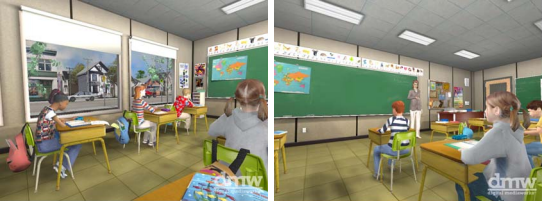
\includegraphics[height=\imgHeightSmall{}]{img/SoA_Rizzo_VirtualClassroom_Cleaned.PNG}}
			\captionof{figure}{Salle de classe virtuelle (Rizzo \textit{et al.})}
			\label{Rizzo_VirtualClassroom}
		\end{minipage}\medskip

		Le matériel utilisé était un HMD avec vision stéréoscopique et capteurs de mouvements ainsi que d'autres capteurs de mouvements sur les bras et les jambes. Ils servent à quantifier le nombre de mouvements de l'enfant et ainsi offrir une métrique supplémentaire.
		
		Un autre outil, développé pour les mêmes raisons que le projet précédent, est le AULA test par Nesplora \cite{Diaz_AulaVRTest}. 
		Son intérêt est l'utilisation du HMD pas uniquement comme périphérique d'affichage mais également comme capteur de mouvements pour quantifier l'attention de la personne (le nombre de mouvements, leur fréquence, mais aussi le temps passé à regarder autre chose). Il ne nécessite donc pas d'autres capteurs de mouvements. La validité de ce test a été étudiée sur un échantillon de 57 enfants (29 sur ce test et 28 sur un test classique) et jugée utile pour compléter un diagnostic de troubles de l'attention.

	\subsection*{VR utilisé pour évaluer l'héminégligence spatiale}

		L'héminégligence spatiale est un des problèmes neurologique le plus étudié à l'aide de la VR (pour l'évaluation et la réhabilitation). Ce trouble apparaît souvent suite à un AVC (Accident Vasculaire Cérébral). Il implique une inattention, ou de la difficulté à répondre aux stimuli apparaissant de l'autre côté de l'hémisphère lésé du cerveau \cite{VARSG4HC1}.
		Katz \textit{et al.} \cite{Katz_CrossStreet} ont réalisé un programme où le patient doit traverser une route dans une réalité virtuelle (figure \ref{Katz_CrossRoad}). Ils ont obtenu des résultats concluant sur l'efficacité de la VR dans le traitement de ce dysfonctionnement. L'asymétrie entre leur angle de déviation ainsi que leur temps de réaction à un stimulus visuel ou auditif sont des métriques pouvant être utilisées pour mesurer le progrès d'un patient.
		
		\begin{minipage}{\linewidth}
			\makebox[\linewidth]{
				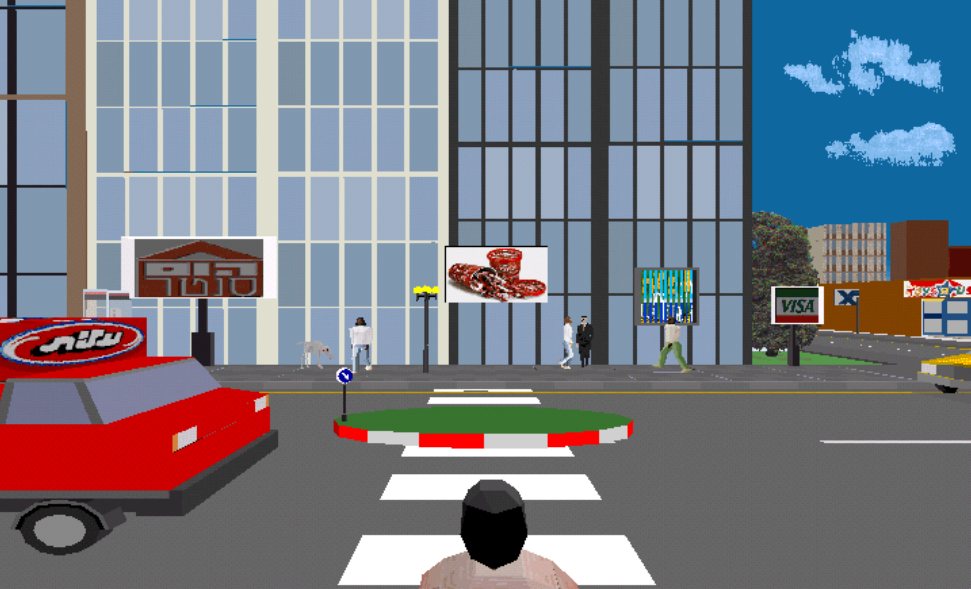
\includegraphics[height=\imgHeightSmall{}]{img/SoA_Katz_CrossRoad.PNG}}
			\captionof{figure}{Environnement virtuel recréer pour simuler la tâche "traverser une route" (Katz \textit{et al.})}
			\label{Katz_CrossRoad}
		\end{minipage}\medskip
		
		%TODO: Lire "Katz_CrossStreet" et étoffer

\section{Simulation 3D en neuropsychologie et neuroréhabilitation suite à un AVC}	
	\label{sSoaSim3DNeuropsyNeuroRehabAVC}
	Entre 30 et 66\% des personnes atteintes d'un AVC ne sont plus capables de se servir de l'un de leur bras dû aux lésions créées dans le cortex cérébral \cite{VanderLee_ForcedUse}. Le succès d'une neuroréhabilitation est directement lié à une grande quantité de mouvements du membre parétique (plus de 20 heures pour une amélioration significative) d'après Cochrane \cite{Cochrane_Intervention4MotorApraxia}). Ils sollicitent la neuroplasticité du cerveau, qui est sa capacité à créer, modifier et détruire des connexions entre les neurones \cite{Grefkes_CorticalReorganization}.

	Les systèmes de VR, pour la neuroréhabilitation cognitive et motrice suite à un AVC, sont en train de se répandre rapidement et de nombreuses plateformes sont en cours de développement. 
	Les avantages de l'utilisation de la réalité virtuelle qui peuvent être trouvés dans la littérature scientifique sont les suivants \cite{VARSG4HC1}:
	\begin{itemize}
		\item \textbf{Neuroplasticité --} Permet l'utilisation de scénarios basés sur des principes facilitant la neuroplasticité tels que l'intensité d'un exercice, sa fréquence, etc.;
		\item \textbf{Entraînement personnalisé --} Offre la possibilité au thérapeute de pouvoir personnaliser l'intensité et la difficulté de l'entraînement d'après les besoins du patient;
		\item \textbf{Objectifs motivants --} L'exercice peut définir des tâches ayant pour but de ré-entraîner des capacités spécifiques (\textit{e.g.}, atteindre un objet, le saisir) tout en étant dans un scénario ludique afin de maintenir une grande implication du patient; %TODO: Parler de ça ?: In particular, al of sutdies evidenced the of VR in augmenting the sense of Presence[49, 50] and the optimal experience [25] in the rehabilitative process.
		\item \textbf{Mesures quantitatives --} À l'aide de capteurs intégrés aux systèmes de réalité virtuelle, il est possible d'avoir un enregistrement précis des actions effectuées par le patient et de se servir de ces informations pour mesurer les performances et le progrès;
		\item \textbf{Entraînement d'activité de la vie quotidienne --} La réalité virtuelle permet la réalisation d'exercices de réhabilitation dans un scénario de tâches de la vie quotidienne (\textit{e.g.}, payer au supermarché).	
	\end{itemize}
	%TODO: Mettre ça ?: The capacity of VR-based systems as a facilitation tool for functional recovery by engaging brain circuits, such as motor areas, has been demonstrated [2].

	Une méta-analyse a été réalisée par Saposnik et Levin \cite{Saposnik_VR4StrokeRehab} sur 12 études (195 participants) afin de déterminer les bénéfices de l'utilisation de la VR pour le rétablissement de la motricité du bras (suite à un AVC). Les résultats obtenus ont permis de montrer que l'ajout d'exercices de réalité virtuelle dans une thérapie augmente son efficacité.
	\\
	
	Dans cette section sont présentés plusieurs plateformes de VR pour la réhabilitation des membres supérieurs et de la main.

	%TODO: Placer ça dans l'intro aussi? : "In the last decade, the use of VR in neurorehabilitation rose a significant way and a n increasing number of experimental findings suggested that this technology can positively impact upon cognitive and motor functional recovery [1-3, 33, 37, 52, 57]. The rationale for the use of VR systems in the rehabilitation field is based on a series of advantages widely documented in the scientific literature:

	\subsection*{Broeren \textit{et al.} - VR et haptique, réhabilitation motrice du bras d'un patient}
		Broeren \textit{et al.} \cite{Broeren_VRHaptic} ont étudié si un environnement virtuel couplé à un périphérique haptique peu augmenter les fonctions motrices d'un bras parétique de sujets ayant subis un AVC. Le système consiste en un joystick 3D avec retour de force (translations et rotations) ainsi qu'un écran stéréoscopique (avec lunettes) pour afficher l'EV en 3D (figure \ref{Broeren_System}).
		
		Le but du programme est de frapper une balle afin qu'elle casse des briques pour gagner des points dans une zone en 3D. Si la balle n'est pas renvoyée, le patient perd des points. L'environnement 3D contient la balle, des briques et un affichage du score, le tout étant à l'intérieur d'un cube. 
		
		L'étude est basée sur un sujet et un groupe de contrôle de 9 personnes saines d'une moyenne de 50 ans. Elle a été effectuée sur quatre semaines où 12 sessions de 90 minutes ont été effectuées. Elle a montré une amélioration de la dextérité et de la force, jugées utiles dans des applications quotidiennes par le patient.
		
		\begin{minipage}{\linewidth}
			\makebox[\linewidth]{
				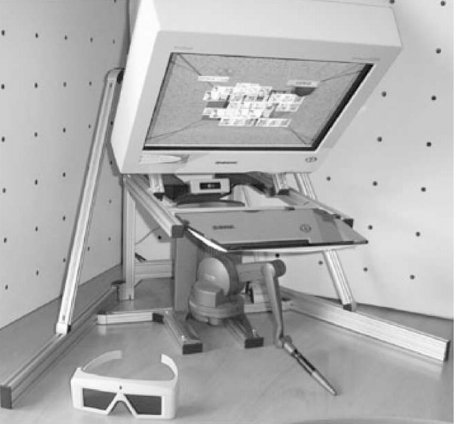
\includegraphics[height=\imgHeightSmall{}]{img/SoA_Broeren_SystemHaptic.PNG}}
			\captionof{figure}{Broeren \textit{et al.} - Système haptique avec vision stéréoscopique utilisé.}
			\label{Broeren_System}
		\end{minipage}\medskip

	\subsection*{Crosbie \textit{et al.} - VR pour la réhabilitation du bras suite à un AVC}
		Le système développé par Crosbie \textit{et al.} \cite{Crosbie_DevVR4StrokeRehab} utilise un HMD (CyVisor) avec des écouteurs intégrés qui affiche un environnement virtuel composé d'objets simples et familiers. Il utilise également un gant "5DT data glove" pour faciliter l'interaction manuelle ainsi que des capteurs de position et d'orientation à quatre endroits du corps du patient: trois sur le bras et un sur le HMD pour augmenter l'immersion (figure \ref{Crosbie_Devices}).
		
		\begin{minipage}{\linewidth}
			\makebox[\linewidth]{
				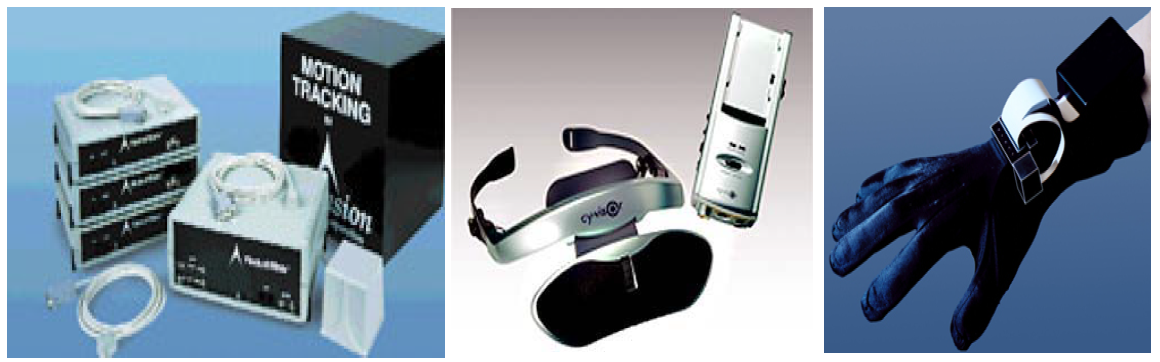
\includegraphics[height=\imgHeightSmall{}]{img/SoA_Crosbie_Devices.PNG}}
			\captionof{figure}{Périphériques utilisés pour l'exercice de réhabilitation (Crosbie \textit{et al.})}
			\label{Crosbie_Devices}
		\end{minipage}\medskip
		
		Le patient est immergé dans l'environnement virtuel où une copie de la table est présente. Il contient également de nombreux objets ainsi qu'une représentation de son bras. Il est alors demandé à l'utilisateur de saisir ces objets et de les déplacer (figure \ref{Crosbie_VE}).

		\begin{minipage}{\linewidth}
			\makebox[\linewidth]{
				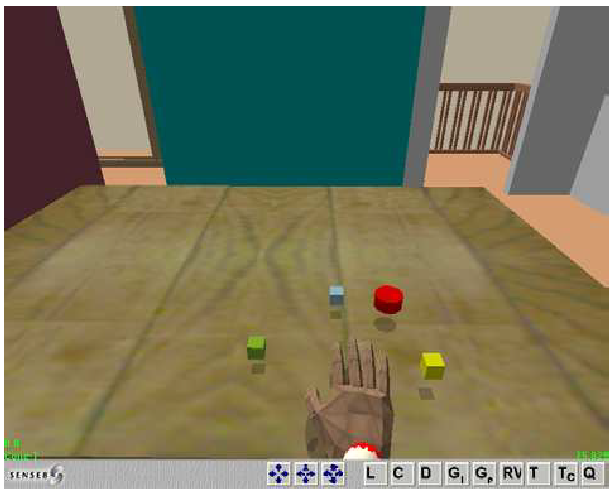
\includegraphics[height=\imgHeightSmall{}]{img/SoA_Crosbie_VE.PNG}}
			\captionof{figure}{Environnement virtuel avec table, objets et représentation du bras (Crosbie \textit{et al.}).}
			\label{Crosbie_VE}
		\end{minipage}\medskip
		
		Tous les éléments du système ainsi que les interactions de l'utilisateur sont mesurables. La réhabilitation peut alors être quantifiée sur la base de ces mesures.
		
		Une étude avec deux groupes de sujets a été menée \cite{Crosbie_RandomizedStudy}. Le premier groupe a effectué une réhabilitation avec ce système et le deuxième, une réhabilitation traditionnelle. Les mesures des capacités motrices n'ont pas montré de différences effectives entre les groupes. L'étude a donc montré l'utilisation possible de la réalité virtuelle pour ce cas de réhabilitation. Si les résultats ne sont pas meilleurs, ils sont cependant plus complets (grâce à l'enregistrement des mouvements de l'utilisateur) pour de futures analyses.
		
		Une autre étude \cite{Crosbie_UserPerpective} a également été réalisée auprès des utilisateurs afin d'analyser la qualité de l'immersion et l'effort ressenti avec, notamment, l'échelle de Borg. L'utilisation de la réalité virtuelle peut en effet provoquer chez certaines personnes des nausées, maux de tête et vertiges.
		%TODO: Semble non finit

	\subsection*{Boian \textit{et al.} VR pour la réhabilitation des mains}
		Le système de VR réalisé par Boian \textit{et al.} pour la réhabilitation des mains \cite{Boian_HandRehab} utilise un \textit{CyberGlove} et un gant haptique "\textit{Rutgers Master II-ND}". Le but de ce système étant d'augmenter la plage de mouvement, la vitesse, l'indépendance et la force de chaque doigt (figure \ref{HapticGlove}).
		
		Une étude a été réalisée \cite{MeriansSensorimotorTraining} pour tester l'efficacité des entraînements utilisant ce système. Les mesures effectuées sur les huit sujets ont montré une amélioration de la plage de mouvement des doigts, de leur force, de leur capacité à bouger indépendamment et de leur vitesse. Leur conclusion est qu'il est difficile qu'un patient ai suffisamment de pratique pour améliorer ses capacités, c'est pourquoi l'utilisation de la VR peut être une bonne solution pour maximiser le temps du patient et du thérapeute.


		\begin{minipage}{\linewidth}
			\makebox[\linewidth]{
				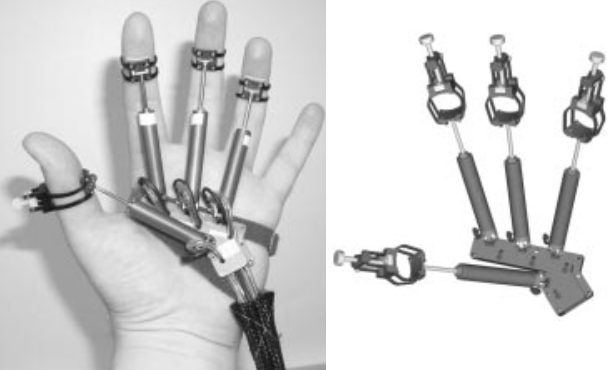
\includegraphics[height=\imgHeightSmall{}]{img/SoA_Boian_HapticGlove.PNG}}
			\captionof{figure}{Rutgers Master II-ND, gant avec retour de force.}
			\label{HapticGlove}
		\end{minipage}\medskip
		
		Pour chacune de ces caractéristiques, un exercice est réalisé dans une réalité virtuelle. Ils comprennent une représentation de la main ainsi que d'autres éléments sur un fond vert. Le gant haptique n'est utilisé que pour la force, les autres exercices utilisaient le \textit{CyberGlove} (figure \ref{Boian_VR}).
		
		\begin{minipage}{\linewidth}
			\makebox[\linewidth]{
				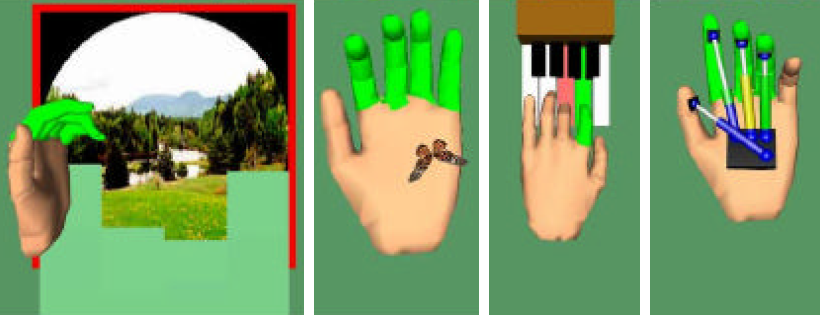
\includegraphics[height=\imgHeightSmall{}]{img/SoA_Boian_VR_FlatCleaned.PNG}}
			\captionof{figure}{Boian \textit{et al.} - Aperçu des exercices. Dans l'ordre de lecture: Plage de mouvement; vitesse; indépendance; force.}
			\label{Boian_VR}
		\end{minipage}\medskip
		
		Sur quatre patients, tous ont significativement amélioré l'indépendance de leurs doigts (possibilité d'en bouger un individuellement), trois ont augmentés leurs vitesses et leurs plages de mouvement. Le gain en force était relativement faible dû à une malfonction du gant.

\section{SGs pour la réhabilitation d'un membre suite à un AVC}

	\label{sSoaSGNeuroRehab}
%TODO: Parler de ça ?: In particular, there is evidence for the effectiveness of such approaches for the rehabilitation of upper limbs in patients with stroke [14, 31, 37, 57]."
	Comme expliqué dans la section précédente, pour qu'une réhabilitation soit efficace, il faut beaucoup de pratique et des exercices répétés. La thérapie en elle-même peut alors être vue comme ennuyante même si elle se déroule dans une réalité virtuelle. L'ajout d'éléments ludiques se prête bien aux thérapies utilisant la réalité virtuelle (l'immersion dans un environnement virtuel et différents périphériques d'interaction déjà présents). Ces éléments ludiques peuvent ajouter de l'intérêt à ces exercices. Mais la motivation, qui est un des facteurs clés des systèmes utilisant la réalité virtuelle pour la réhabilitation \cite{Robertson_AugmentedFeedback}, peut être largement augmentée dans le cas d'un jeu sollicitant ces exercices pour progresser. Les personnes effectuant une réhabilitation apprécient le challenge \cite{Burke_DesigningEngagingPlayableGames4Rehab}, or il est rarement présent dans les thérapies classiques ou les exercices simples en réalité virtuelle. De plus, le côté ludique ne concerne plus uniquement de petits éléments de l'exercice. C'est l'exercice qui, aux yeux du patient, doit être un élément du jeu. C'est le principe des \textit{serious games} (SG) qui peuvent comporter toutes les mécaniques d'un jeu habituel appliquées à un aspect sérieux. Dans cette section sont présentés différents SG où l'aspect sérieux est la pratique d'exercices de réhabilitation. Ainsi, la thérapie, qui pouvait être vue comme une série longue et répétitive de mouvements, peut être perçue comme une activité agréable. De nombreux jeux actuels arrivent à maintenir le joueur engagé durant de longues périodes malgré que l'interaction ne se base que sur quelques boutons appuyés de façon répétitive.
	L'utilisation de robots pour assister les mouvements est l'une des approches prometteuses pour les patients avec une atteinte modérée ou sévère de la motricité. Ils permettent d'accompagner le patient s'il ne fournit pas une force suffisante ou de corriger ses mouvements si nécessaire. Ils permettent également de mesurer les détails des mouvements du patient pour mesurer sa progression.

	\subsection*{\textit{ARMin} et SGs} 
		"\textit{ARMin}" \cite{Nef_ARMinRobot} est un exosquelette robotisé permettant de bouger les articulations de l'épaule, du coude et du poignet (figure \ref{Nef_ARMin}).
		
		\begin{minipage}{\linewidth}
			\makebox[\linewidth]{
				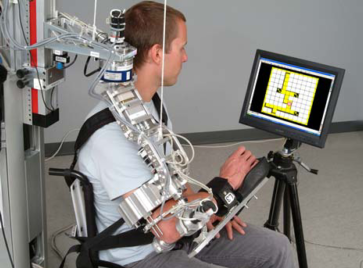
\includegraphics[height=\imgHeightSmall{}]{img/SoA_Nef_ARMin.PNG}}
			\captionof{figure}{Robot \textit{ARMin}, robot de réhabilitation développé à l'\textit{ETHZ}.}%TODO: Expliquer ce qu'est l'ETHZ ? Le mettre dans le lexique ?
			\label{Nef_ARMin}
		\end{minipage}\medskip
		
		Il est couplé à un écran et des haut-parleurs et permet de réaliser des exercices (non détaillés dans ce rapport) et deux jeux pour la réhabilitation du bras (figure \ref{Nef_Scenarios}). Dans le premier jeu, une boule se déplace d'après les mouvements du bras du patient. Le but étant d'amener la boule en haut du labyrinthe, la balle ne devant pas toucher les bords. Dans le deuxième jeu, le patient déplace une poignée à l'écran afin d'attraper une boule qui tombe. La poignée passe du rouge au vert et un \textit{feedback} sonore se produit si le patient attrape la balle.
		
		\begin{minipage}{\linewidth}
			\makebox[\linewidth]{
				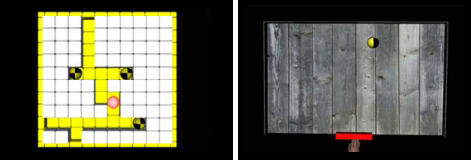
\includegraphics[height=\imgHeightSmall{}]{img/SoA_Nef_Selection.PNG}}
			\captionof{figure}{Fenêtres des jeux de l'\textit{ARMin}. Dans l'ordre de lecture: jeu du labyrinthe; jeu de la boule.}
			\label{Nef_Scenarios}
		\end{minipage}\medskip
		
		L'assistance du robot ou sa résistance peut être réglée par le thérapeute.
		Plusieurs études sans groupe de référence ont tout de même montré qu'une grande utilisation du système peut significativement améliorer les capacités du patient \cite{Nef_EffectsArmTraining, Staubli_EffectsIntensiveArmTraining}.



%"Robotic rehabilitation systems help guide hemiparetic movements actively if adequate motor control is unavailable and show particular promise for patients who may have more severe upper limb impairments [78]."

%TODO Parler de cette étude ? Les jeux ont vraiment l'air trop basique pour être intéressant. Rien de nouveau par rapport à ARMin et SGs...
%\subsection*{UL-EX07 et SGs}
%"In Kim \textit{et al.} [55] the UL-EX07 robot was combined with eight interactive video games as an intervention for 30 hemiparetic participants." "Four of the games developed for this study were purely diagnostic tools; these included flower, paint, joint movement and reach. The remaining four: "pong", "cirular pong", "pinball" and "hand ball" games, were all able to accommodate either bimanual of unilateral therapeutic movements. Difficulty using the UL-EX07 is modulated by adjusting the level of compensation for gravity and active assistance provided by the robot."

%TODO Parler de cette étude ? Les jeux ont vraiment l'air trop basique pour être intéressant. Rien de nouveau par rapport à ARMin et SGs...
%subsection*{Plasma pong, Hummingbird, Virtual Piano, Hammer Task}
%Merians \textit{et al.} [80] ont fait une étude avec des Cyberglove et CyberGrasp (exosquelette robotique pour les doigts). 4 jeux ont été testés :
%Plasma pong
%Hummingbird
%Virtual Piano
%Hammer Task

%TODO Parler de ça ? (Aucune info sur les jeux trouvée...)
%"In Housman \textit{et al.} [50] the results of an intervention using a passive robotic exoskeleton called T-WREX combined with Vu Therapy games was reported in chronic stroke participants. ... Prior to each session Vu Therapy games undergo a software-based calibration by a clinician which adjusts difficulty accordingly."

%TODO Parler de cette étude ? Les jeux ont vraiment l'air trop basique pour être intéressant. Rien de nouveau par rapport à ARMin et SGs...
%Steinisch \textit{et al.} [111] a fait un étude avec un robot passif et 5 jeux vidéos ("Sponge", "Bug hunt", "Twirl", "Grab 2D", "Grab 3D".










%18.5 Virtual Reality and Custom Upper Limb Video Games

% TODO: Trouver où placer ce blabla écologique (du chap 18): "First, the use of rich, multisensory, graphical representations of real world scenarios can provide a more cognitively stimulating and salient experience for the patient. Second, task practice in a simulated environment may provide more ecological validity than practice performed in conventional therapy sessions [100]." 
% TODO: Trouver où placer ce blabla cyber sickness (du chap 18) "Fully immersive systems commonly use head mounted displays thar are sometimes associated with cyber sickness in the elderly population [6, 70]." 

%TODO: Parler d'eux peu-être. Peu d'info on été trouvé sur les jeux en soi. : Sucar \textit{et al.} [113] ont fait une étude comparative entre les thérapies conventionel et un système de jeux vidéos. 8 jeu demandant des taches et mouvements spécifiques.

	\subsection*{Ma et Bechkoum - SGs pour une thérapie basée sur le mouvement suite à un AVC}
		Le but de ce projet est d'encourager les patients à faire leur thérapie de mouvement pour la réhabilitation de leur bras parétique. Ceci est réalisé à l'aide d'un ensemble de SGs où des facteurs tels que la taille des éléments ou la gravité peuvent être réglés afin de s'adapter à leurs capacités \cite{Ma_SG4MovTherapy}. Tous les SGs utilisent un environnement virtuel immersif à l'aide d'un HMD ainsi qu'un retour sonore.
		\\

		\textbf{\textit{Catch-the-orange} --} Dans ce SG, le patient doit ramasser des oranges qui tombent d'un arbre (figure \ref{Ma_CatchOrange}, image de gauche) à l'aide d'un panier. La position et l'orientation du panier sont obtenues via un capteur posé sur un panier réel que le patient doit tenir avec une ou deux mains, en fonction de la thérapie (figure \ref{Ma_CatchOrange}, image de droite). Si le panier est au mauvais endroit, les oranges tombent par terre et sont perdues. S'il est trop incliné celles déjà ramassées peuvent tomber et être également perdues.
		La difficulté est réglable via: un facteur de gravité; la taille des oranges; le laps de temps qui s'écoule entre chaque chute d'orange.
		
		\begin{minipage}{\linewidth}
			\makebox[\linewidth]{
				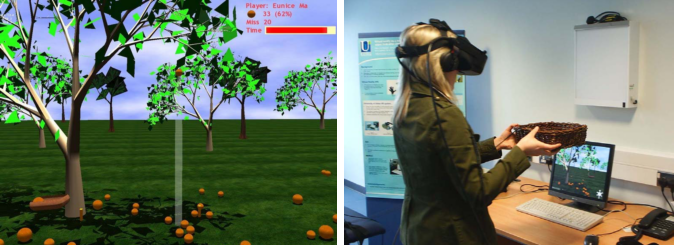
\includegraphics[height=\imgHeightSmall{}]{img/SoA_Ma_CatchOrange.png}}
			\captionof{figure}{Ma et Bechkoum - \textit{Catch-the-orange}. Dans l'ordre de lecture: environnement virtuel; individu en train de jouer.}
			\label{Ma_CatchOrange}
		\end{minipage}\medskip
		
		\textbf{\textit{Fishing game} --} Ce SG est celui le plus apprécié par les patients. Ils sont immergés dans un monde sous-marin et doivent se servir de leurs bras pour attraper des poissons qui nagent (figure \ref{Ma_Fishing}, image de gauche). Le patient voit une représentation de ses deux mains, ce qui est rendu possible grâce à l'utilisation d'un capteur par main (figure \ref{Ma_Fishing}, image de droite). Si une main touche le poisson, il partira en nageant bien plus vite. Cependant, si les deux mains le touchent, il se débattra (retour visuel) puis disparaîtra en incrémentant le compteur de poissons attrapés. La difficulté est réglable via: la taille de la zone (amplitude du mouvement); la vitesse des poissons; leur taille; la taille des mains.

		\begin{minipage}{\linewidth}
			\makebox[\linewidth]{
				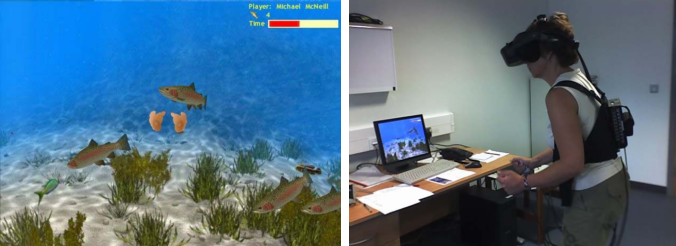
\includegraphics[height=\imgHeightSmall{}]{img/SoA_Ma_Fishing.png}}
			\captionof{figure}{Ma et Bechkoum - \textit{Fishing game}. Dans l'ordre de lecture: environnement virtuel; individu en train de jouer.}
			\label{Ma_Fishing}
		\end{minipage}\medskip
		
		\textbf{\textit{Whack-a-mouse} --} En plus d'améliorer la mobilité, la précision et la vitesse du bras, ce SG a été conçu pour améliorer la discrimination visuelle et l'attention sélective. Ce sont des facteurs importants d'une réhabilitation suite à un AVC pour les patients présentant une héminégligence spatiale. Dans ce SG, une souris apparaît sur une table à un endroit aléatoire et y reste, un certain nombre de secondes, puis disparaît pour réapparaître ailleurs. Le joueur doit frapper la souris avec un marteau contrôlé par la position et l'orientation d'un capteur sur sa main (figure \ref{Ma_Mouse}). Quand la souris est touchée, elle fait en petit cri et devient rouge (retour visuel) avant d'incrémenter le score. La difficulté est réglée via le nombre de secondes où la souris reste.

		\begin{minipage}{\linewidth}
			\makebox[\linewidth]{
				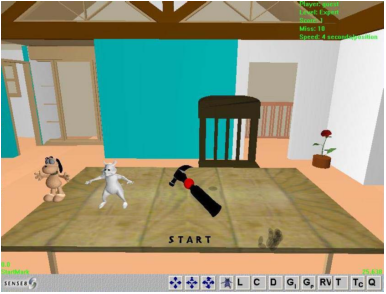
\includegraphics[height=\imgHeightSmall{}]{img/SoA_Ma_WhackAMouse.png}}
			\captionof{figure}{Ma et Bechkoum - \textit{Whack-a-mouse}, environnement virtuel.}
			\label{Ma_Mouse}
		\end{minipage}\medskip

		Les jeux se règlent automatiquement par rapport au profil du patient. Les paramètres cités dans chaque jeu mais également le lieu des stimuli, se règlent en fonction (prenant compte également du côté parétique et de son héminégligence). Des niveaux de difficulté "facile", "intermédiaire" et "expert" sont disponibles. Dans le niveau facile le jeu s'adapte simplement au profil du patient. Dans le niveau intermédiaire, les paramètres changent en cours de partie (plus le patient a du succès, plus la difficulté augmente et inversement). Le niveau expert utilise des éléments malus. Exemple: dans \textit{Whack-a-mouse}, un chien apparaît en même temps que la souris et le joueur ne doit pas se tromper de cible, ce qui fait travailler sa discrimination visuelle.
		\\
		
		Le niveau, le score et la vitesse sont affichés constamment en haut à gauche et, en fin de partie ou en passant au niveau suivant, des informations telles que le score, la précision moyenne et la durée sont affichées sur un écran final. Ces données sont également enregistrées dans un fichier pour régler la difficulté lors de prochaines parties ou pour que le thérapeute les analyse. Pour créer un peu de compétition, le patient peut voir les meilleurs scores de tous les joueurs mais également juste les siens pour chaque niveau et chaque jeu.
		\\
		
		Des tests utilisateurs ont été réalisés sur huit patients entre 43 et 75 ans. Un groupe (quatre patients) faisait une thérapie de mouvement traditionnelle et des SGs et l'autre ne faisait pas les SGs. Il n'est pas précisé la durée des sessions pour chaque groupe. Les tests ont montré un impact positif de l'utilisation des SGs pour améliorer les capacités motrices.

%TODO: Doc non trouvable gratuitement (demande effectuée). Si trouvée, ecrire là dessus
%Crosbie \textit{et al.} ont continuer à faire des SG [23] ("Rabbit chase", "Arrow Attack")

%TODO: Doc non trouvable gratuitement Si trouvée, ecrire là dessus
%TODO: Documenter au moins le produit utilisé -> 20 jeux pour différentes pathologies ! (http://www.gesturetekhealth.com/products-rehab-irex.php)
%Kwon \textit{et al.} [62] ont fait un étude avec un outils clinique de VR "IREX" dévelopé par GestureTek et qui offre 23 jeux de réhabilitation dont 5 pour la réhabilitation des membres supérieurs. Il se sert d'une caméra et de Cybergloves pour capter les mouvements. Le système fournit une variété de feedback incluant des scores ainsi que des diagrammes de progression.

%TODO: Attendre la récéption du 18_89 (demandé via research gate) et éventuellement écrire un truc dessus (semble un peu simple comme jeu)
%\subsection*{Rehabilitation Gaming System}
%"Rehabilitation Gaming System" est développé d'après un projet scientifique, par une collaboration entre des universités et des hôpitaux en Espagne. 
%http://rgs-project.eu/games
%The Rehabilitation Gaming System (RGS) is a novel and highly innovative ICT Virtual Reality (VR) tool for the rehabilitation of motor deficits of the upper extremities after a brain lesion due to stroke. The system deploys an individualized game training that combines movement execution with the observation of a correlated action by virtual limbs that are displayed in a first-person perspective. (read more description below)
%Cameirao et al on fait une étude avec "Rehabilitation Gaming System" [15, 89] se servant de "Data glove" pour récupérer les flexions des doigts

	\subsection*{\textit{Voracy Fish} \cite{VoracyFish}}%Le projet MoJOS n'existe plus. Même l'adresse http://www.mojos.fr/home/ redirige sur http://www.voracy.com/
		Ce projet a également pour but la réhabilitation du bras chez les personnes ayant eu un AVC. Il est créé par \textit{Brain  e-NOVATION} \cite{BrainENOVATION} étant un laboratoire mettant en commun l'expertise médicale de "l'Institut du Cerveau et de la Moelle Épinière" (ICM) et l'expertise informatique orientée santé du groupe français \textit{GENIOUS}. Le SG se joint à la plateforme \textit{GENIOUS GAMe-S} proposant un espace patient et un espace thérapeute avec une liaison directe entre les exercices effectués par le patient chez lui et l'hôpital pour que le thérapeute puisse voir d'une part la progression et d'autre part lui communiquer des informations, planifier des séances ou directement changer la rééducation. Ce projet a été récompensé à de nombreuses reprises, notamment par un trophée e-santé en 2013 pour son travail dans la catégorie "Autonomie et maintien à domicile", en étant finaliste "e-virtuoses" en 2013 dans la catégorie "\textit{serious game} Santé", ou encore par le titre de meilleur projet industriel "e-santé" 2012.
		\\
		
		Pour le matériel, les mouvements du patient sont récupérés à l'aide d'une \textit{Kinect} (caméra développée par Microsoft permettant la reconnaissance d'un mouvement du corps dans un environnement en 3D \cite{Kinect_website}), le jeu est affiché sur un écran et des haut-parleurs sont présents pour l'audio (figure \ref{FigVoracyFish}, image de droite). Le patient peut effectuer les mouvements en l'air ou le bras posé sur une table. Il peut également guider son bras parétique avec son autre bras si besoin. L'avantage de cette solution est qu'elle utilise des dispositifs tout public et permet la réalisation des exercices à la maison.
		\\
		
		Dans le jeu, le patient incarne un poisson dans un environnement 3D contenant des éléments audio (figure \ref{FigVoracyFish}, à gauche). Son but étant de manger d'autres poissons et de trouver des trésors. Plus il mange de poissons, plus il grandit et plus il monte dans la chaîne alimentaire et peut manger de plus gros poissons. Le poisson se déplace constamment et le joueur peut influer sur la direction (verticale et horizontale) à l'aide de la position de son bras.
		\\
		
		Ce jeu peut également se jouer à plusieurs joueurs et avec d'autres périphériques d'entrée, tels qu'une tablette tactile ou une souris. Le but du joueur est alors de manger ses adversaires. Ainsi le patient peut effectuer sa thérapie (avec la \textit{Kinect} \cite{Kinect_website}) à la maison tout en s'amusant avec ses proches (qui utilisent une tablette ou une souris).\medskip
		
		\begin{minipage}{\linewidth}
			\makebox[\linewidth]{
				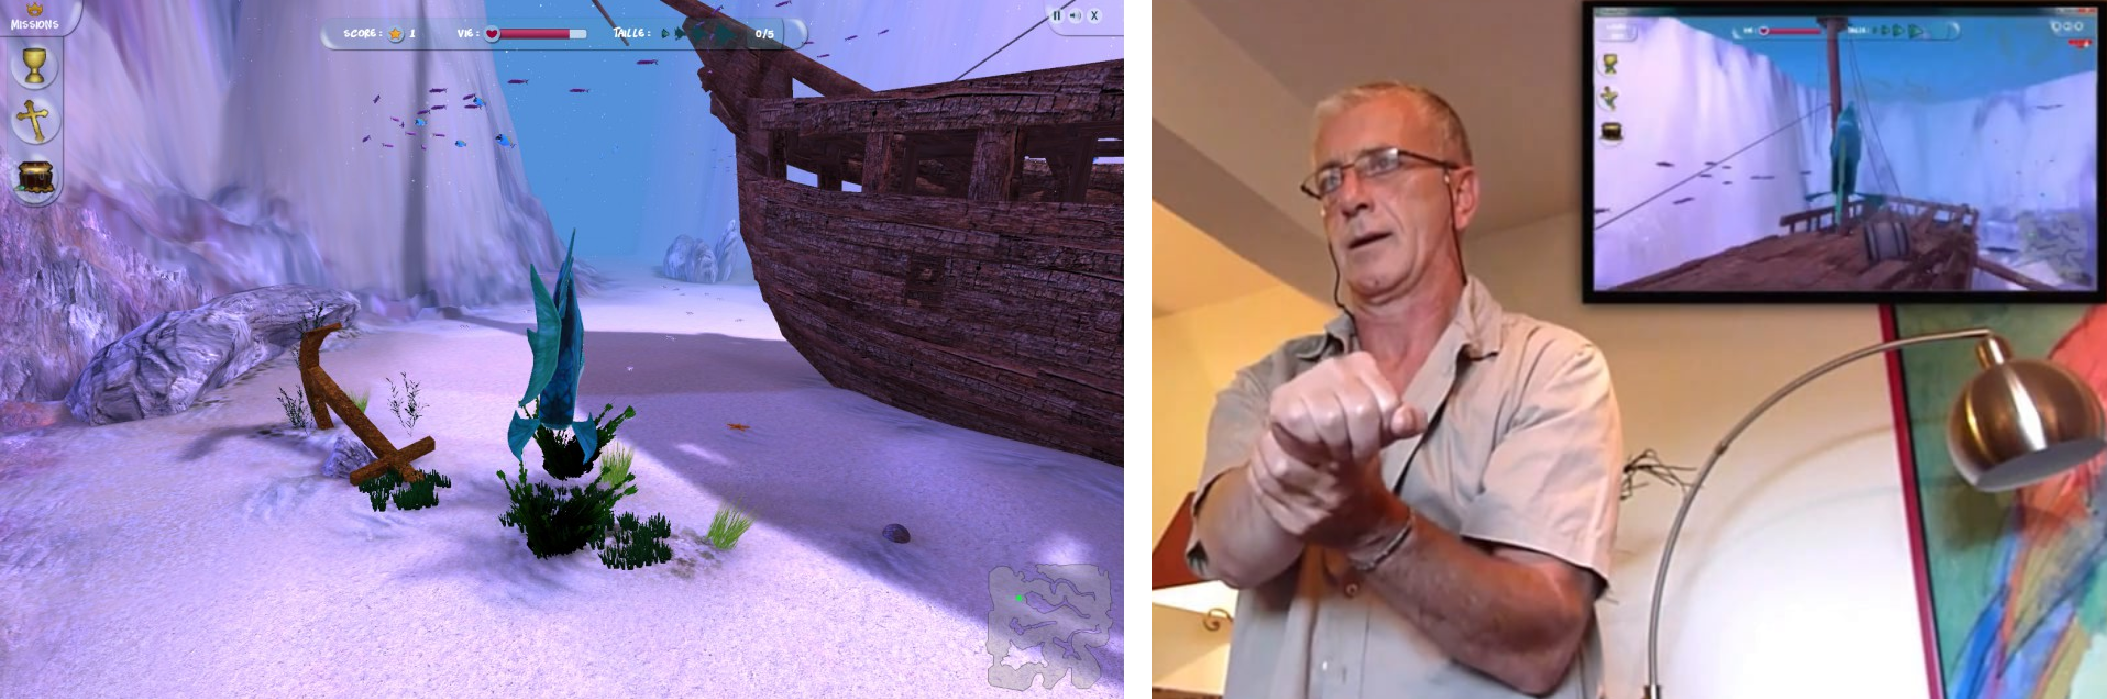
\includegraphics[height=\imgHeightSmall{}]{img/SoA_VoracyFish.png}}
			\captionof{figure}{\textit{Voracy Fish}. Dans l'ordre de lecture: environnement virtuel; individu en train de jouer.}
			\label{FigVoracyFish}
		\end{minipage}\medskip
		
		Aucune d'études clinique n'a encore été effectuée, mais c'est un des prochains objectifs du groupe \textit{Brain e-NOVATION} \cite{ICM_Strokes}.
	
	\subsection*{Neurorehabilitation Training Toolkit (NTT)}
		Ce concept a pour but une réhabilitation motrice des bras à domicile avec une installation à faible coût \cite{Bermudez_NTT}. Il est réalisé par l'université Da Madeira au Portugal et consiste en une application web accessible depuis un navigateur internet pour fournir le SG, les instructions et les retours d'informations. Il exige également que le PC ai deux souris (une extension a, par la suite, été réalisée pour être utilisée avec une \textit{Kinect} \cite{Bermudez_NTTToKinect}). Une souris sera utilisée par main, celles-ci étant posées sur la table, et a donc un support contre la gravité. La réhabilitation se fait à l'aide de mouvements répétitifs dans le but d'augmenter la coordination, la synchronisation des bras et leur précision.
		\\
		
		Dans le jeu, le patient voit son avatar aux commandes d'un parapente (figure \ref{Bermudez_NTT}, image de gauche) et peut contrôler sa direction à l'aide d'une différence de position verticale entre les mains (figure \ref{Bermudez_NTT}, image de droite), comme s'il tirait sur les poignées du parapente. Le parapente avance à vitesse constante, le but étant de collecter le plus de ballons possible. Cette mécanique de jeu est choisi afin que le patient puisse compenser les mouvements réduits et peu précis du bras parétique avec l'autre. Pour le scénario, le joueur doit retrouver sa maison en avançant de niveau en niveau (il faut récupérer assez de ballons pour passer au niveau suivant). Le jeu commence par un tutoriel. Le jeu essaie d'utiliser le plus de repères et de modalités de retour possibles pour s'assurer que l'utilisateur comprenne l'influence de ses actions et ne se perde pas. Par exemple, à l'écran, une boussole montre la direction du prochain ballon et une image montre le mouvement à effectuer pour aller dans cette direction.
		\\
		
		Quatre paramètres peuvent être modifiés pour adapter la difficulté: la vitesse; la vitesse de rotation; la distance minimale pour collecter un objet; la distance entre les objets à collecter.\medskip
				
		\begin{minipage}{\linewidth}
			\makebox[\linewidth]{
				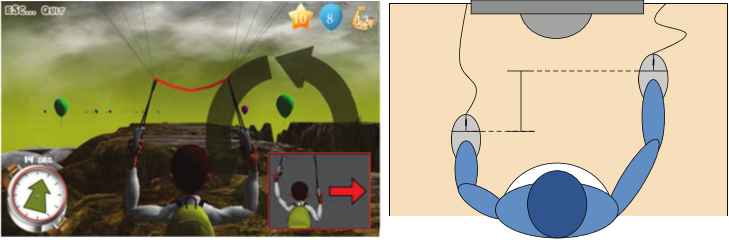
\includegraphics[height=\imgHeightSmall{}]{img/SoA_Bermudez_Edited.png}}
			\captionof{figure}{NTT. Dans l'ordre: interface et environnement virtuel; installation du patient en jeu.}
			\label{Bermudez_NTT}
		\end{minipage}\medskip		
		
	\subsection*{Stroke Recovery with Kinect}
		Ce projet développé par "Microsoft Research"\cite{MicrosoftResearch} consiste en trois programmes de réhabilitation du bras à l'aide d'une Kinect \cite{Microsoft_StrokeRecovery}. Les programmes sont les suivants:
		\begin{itemize}
			\item Un test classique où le patient doit prendre des blocs et les mettre dans une boîte en un temps donné, réalisé dans une réalité virtuelle (figure \ref{MicrosoftResearch_StrokeRecovery}, image de gauche). Le plus de cette utilisation est l'établissement direct d'un score après une session de jeu et la visualisation de la progression au fil des parties;
			\item Un exercice où le patient doit imiter les mouvements affichés à l'écran (figure \ref{MicrosoftResearch_StrokeRecovery}, image du centre). Il reçoit un score basé sur son succès d'après l'échelle de Fugl-Meyer, qui est la mesure quantitative la plus utilisée pour mesurer le progrès d'une réhabilitation pour des patients hémiplégiques \cite{FuglMeyerAssesment};
			\item Un SG dans l'espace où le patient entraîne ses réflexes en guidant un vaisseau spatial horizontalement (via des mouvements horizontaux des bras) pour éviter des astéroïdes (figure \ref{MicrosoftResearch_StrokeRecovery}, image de droite).
		\end{itemize}
		Tous les programmes sont affichés sur un écran (pas d'utilisation de HMD).\medskip
		
		\begin{minipage}{\linewidth}
			\makebox[\linewidth]{
				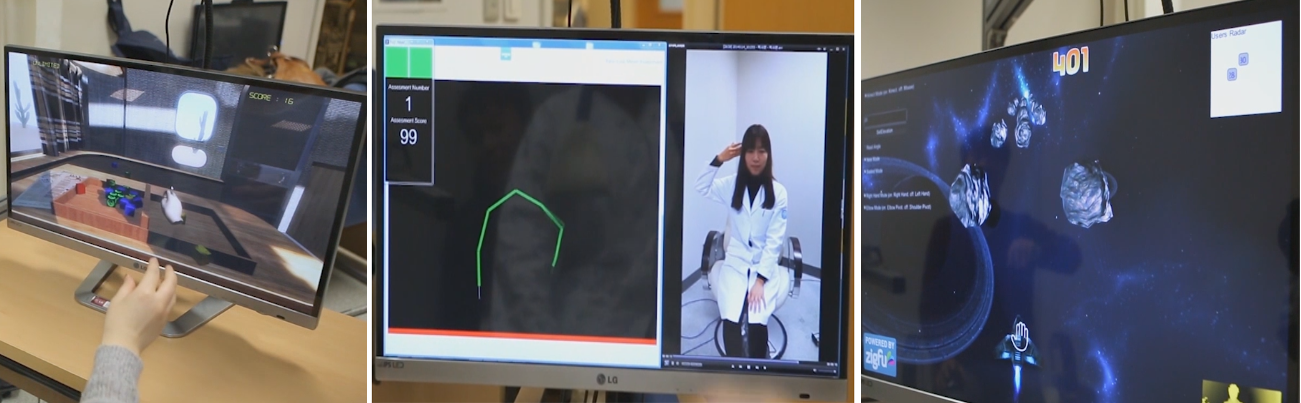
\includegraphics[height=\imgHeightSmall{}]{img/SoA_MicrosoftResearch_StrokeRecovery_Resized.png}}
			\captionof{figure}{Stroke Recovery with Kinect. Dans l'ordre de lecture: test classique; imitation de mouvements; SG.}
			\label{MicrosoftResearch_StrokeRecovery}
		\end{minipage}\medskip
		
		Objectifs à long terme:
		\begin{itemize}
			\item Intégration d'un aspect social pour faire des parties à un contre un et ainsi faire augmenter la motivation;
			\item La construction d'une communauté où ils pourront communiquer leurs problèmes et recevoir des encouragements et de l'aide;
			\item Permettre au personnel médical de contrôler l'avancement des patients depuis leur bureau et de communiquer directement avec eux;
			\item Utilisation d'autres technologies Microsoft, notamment de Cloud pour intégrer du \textit{machine learning}.%TODO: Ajouter dans le lexique ?
		\end{itemize}
		Le point important de ce projet est qu'une référence du domaine informatique tel que Microsoft s'intéresse à ce domaine. Avec de tels moyens, les SGs développés pourront potentiellement être de grande qualité.
				
%\section{SGs pour la réhabilitation des jambes}
	%TODO: Étoffer l'intro
	%Dans cette section est présenté les SGs liés à la neuro-réhabilitation des membres inférieurs, ce sont donc les SGs qui, d’un point de vue but et profil patient sont les plus proche de celui à développer. La complexité de conception pour un SG utilisant les jambes se situe en trois points. Le premier est qu’il est plus difficile de concevoir un jeu avec une interaction basée sur les jambes que sur les bras. Le deuxième point est que les projets cités ne souhaitent principalement réapprendre qu’un mouvement qui est la marche, on ne demande donc aucune autre interaction des membres inférieurs. Le troisième est que si le patient est debout, il doit s’accrocher à des rampes et on exclue alors toute interaction des membres supérieurs.
				
	\subsection*{Gabarello}
		Ce SG est développé pour une utilisation avec le "Lokomat". Ce dernier étant un robot de réhabilitation des jambes contenant principalement un tapis roulant, un exosquelette et un système de soutien du poids du patient développé par \textit{Hocoma} \cite{Lokomat_Brochure} (figure \ref{Lokomat}). Ce SG est destiné essentiellement aux enfants et a été conçu en tant que tel. Le développement a été réalisé par l'université des Arts de Zürich (spécialisation "Game Design") en coopération avec le Kinderspital à Zürich, l'institut de Neuropsychologie de l'université de Zürich et le laboratoire "Sensory Motor Systems Lab" à l'ETHZ.\medskip
		
		\begin{minipage}{\linewidth}
			\makebox[\linewidth]{
				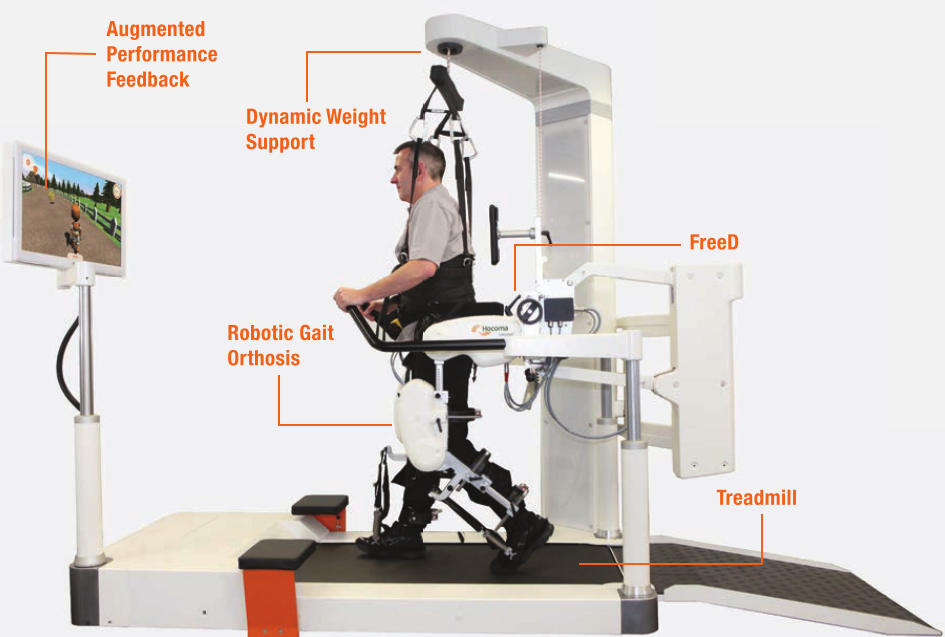
\includegraphics[height=\imgHeightMedium{}]{img/SoA_Lokomat.png}}
			\captionof{figure}{Lokomat, robot de réhabilitation développé par \textit{Hocoma}.}
			\label{Lokomat}
		\end{minipage}\medskip%TODO: Trouver une image avec un enfant du coup ?
		
		Le but du jeu est de collecter des fleurs à la surface d'une planète. Les joueurs contrôlent un astronaute marchant sur celle-ci. En fournissant plus d'effort, les jambes de l'avatar vont grandir (phase active, figure \ref{Gabarello}, image de gauche), et en en fournissant moins, elles vont rapetisser (phase passive, figure \ref{Gabarello}, image de droite). Plus les jambes sont grandes, plus les fleurs récoltées rapportent de points. Avoir de grandes jambes permet aussi de monter sur des plateformes, d'y rester ainsi que de sauter sur les suivantes. L'avatar n'a que trois états qui correspondent au degré d'activité du patient. La synchronisation entre la participation du patient et de l'avatar dure un pas. La force mise par le patient est détectée à l'aide de capteurs directement présents sur le Lokomat \cite{Labruyere_LokomatGabarello}.\medskip
		
		\begin{minipage}{\linewidth}
			\makebox[\linewidth]{
				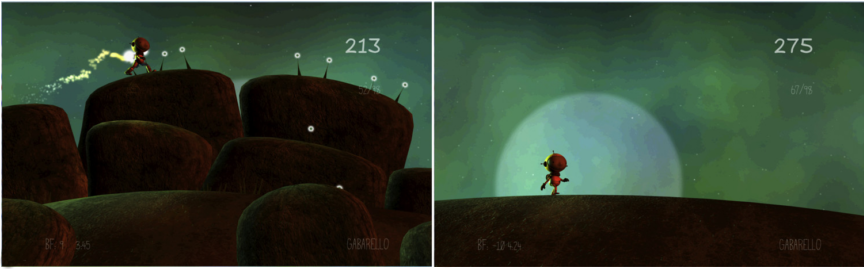
\includegraphics[height=\imgHeightSmall{}]{img/SoA_Lokomat_Gabarello_Cleaned.png}}
			\captionof{figure}{Gabarello. Dans l'ordre de lecture: phase active; phase passive.}
			\label{Gabarello}
		\end{minipage}\medskip
		
		Une étude a été réalisée pour savoir si un enfant peut modifier son niveau de participation pendant un scénario. Les résultats ont montrés qu'il était possible pour eux de modifier leur force durant un exercice, cependant leurs aptitudes cognitives et motrices vont déterminer s'il est capable d'identifier le besoin \cite{Labruyere_LokomatGabarello}.
		\\
		
		D'autres SG fonctionnent avec le Lokomat et font partie du "Challenge package", cependant peu d'informations ont été trouvées \cite{Lokomat_Brochure}. Ils semblent tous se baser uniquement sur le mouvement des jambes (leur synchronisation pour un jeu de vol, la force mise dans le mouvement pour un jeu de course ou encore la trajectoire des pieds) \cite{Lokomat_FlyingGame}. Les jeux semblent contenir des graphismes élaboré, cependant l'interaction de l'avatar et ses déplacements sont saccadés et non cohérent avec son environnement. %TODO Trouver plus d'infos
		
		%TODO Parler de ce projet ou d'un autre (pas faire de sous-section que pour le Lokomat...) :
		%\subsection*{Grail / Stable / CAREN / V-Gait / ...}
		%Projet riche avec beaucoup de périphériques et application dont SG avec de beaux graphismes. Très peu d'infos trouvées sur les SGs...
		
		%http://www.motekmedical.com/products/grail-gait-real-time-analysis-interactive-lab/
		%http://www.motekmedical.com/solutions/rehabilitation/#

			
	\chapter{Analyse}
		Dans cette section sont identifiés les points importants qu'il ont été analysés avant de débuter à la conception du jeu. Premièrement, il est expliqué dans la section \ref{sAnaEtatDesLieux} la situation initiale avec un état des lieux afin de préciser où le projet commence, quels sont les composants existants ainsi que leurs interactions. Deuxièmement, les objectifs du projet de recherche et développement (projet R\&D) englobant sont décrits dans la section \ref{sAnaDescriptionObjectifsCTI} avec de premières pistes pour y répondre. Ces dernières étant issues de l'état de l'art où de nouveaux documents. Troisièmement, la section \ref{sAnaContraintes} détaille les contraintes fixées à ce projet (principalement imposées par les composants ou encore le contexte d'utilisation). Finalement, un condensé de tous les points importants à prendre en compte lors de la conception d'un SG de neuroréhabilitation sont listés dans la section \ref{sAnaGameConceptPointsImportant}.
\section{Contexte initial}
	\label{sAnaEtatDesLieux}
	Ce travail de Master précède un projet R\&D. Il fait suite à un autre projet de recherche I2 "SG4R" dont le but était de créer une plateforme de SG. Il est donc important de spécifier ce qui existe actuellement et de définir ce qui doit être fait dans le cadre de ce travail. Voici une liste des composants déjà réalisés ainsi que leur état d'avancement:
	\begin{itemize}
		\item \textbf{LHS --} Le LHS \cite{LHS_website} est le robot de réhabilitation utilisé dans ce projet comme périphérique de réhabilitation. Il est actuellement opérationnel et déjà utilisé par des patients sélectionnés dans le cadre de tests cliniques (utilisant des exercices déjà configurés et validés par le domaine médical et non les SGs). De nombreux algorithmes pour différents types de mouvement y sont présents, mais pas encore celui de la marche qui doit être développé durant le projet R\&D. De plus ample informations sur le périphérique sont présentés dans la section \ref{sAnaContraintes};
		
		\item \textbf{IHM --} L'interface homme machine livrée avec le produit LHS permettant au thérapeute de rentrer les données du patient, de lui configurer et choisir des exercices et également de modifier leurs paramètres en cours d'exécution ou de les interrompre. Une communication entre la IHM et les SGs existe déjà mais très peu de données du SG sont remontées à la IHM;
		
		\item \textbf{Noyau Temps Réel --} Ce noyau garantit de gérer le LHS avec un nombre de millisecondes donné. C'est lui qui remonte les données des capteurs. Une communication entre les SG et l'application temps réel tournant sur ce noyau existe déjà. Cette communication est bidirectionnelle et permet de lire les valeurs des capteurs ou autres entrées prétraitées à l'aide d'algorithmes prenant en compte l'anatomie du patient (\textit{e.g.}, position des pieds) mais également d'écrire des valeurs telles que la difficulté de pédalage (\textit{e.g.}, dut à la pente);
		
		\item \textbf{Communication --} Une API de communication existe mais est très sommaire. Elle a été conçue pour être fonctionnelle avec différents périphériques de réhabilitation;
		
		\item \textbf{Plateforme de SG avec mode \textit{master} et \textit{slave} --} Une plateforme permettant l'accès à quatre SGs fonctionnels, travaillant des exercices différents. Le projet SG4R ne devant pas être lié uniquement au robot LHS, cette plateforme est générique et peut être exécuté d'après deux modes: "\textit{master}", où la plateforme lance l'interface graphique permettant de choisir les jeux; "\textit{slave}", où la plateforme est lancée en arrière-plan et attend que la IHM lui demande de lancer un jeu;
		
		\item \textbf{SGs existants --} Quatre SGs ont été développés à l'aide du moteur de jeu \textit{Unity} \cite{Unity_website} (les scripts ont été écrits en C\# \cite{CSharp_website}) en tant que prototypes afin de les faire valider par le personnel médical. Ces SGs couvraient différents types de mouvement, interactions additionnelles, types de graphisme, types d'immersion et mécaniques de jeu ou d'adhérence. Ces SGs ont impliqué du matériel supplémentaire: un micro ou une souris (améliorée en un bouton tenant mieux en main) et un HMD (casque de réalité virtuelle). Le HMD utilisé est l'\textit{Oculus Rift}, kit de développement 2 (\textit{Oculus Rift DK2}) \cite{OculusDk2_website}.
		Une description plus précise de \textit{Unit}y et de l'\textit{Oculus Rift} est présente dans la section \ref{sAnaContraintes};
		\begin{itemize} 
			\item \textbf{Bike Rehab --} Seul SG en 2D, de style \textit{cartoon}, se passant dans une Italie caricaturée. Le but du jeu est de livrer des pizzas  à vélo en arrivant le plus propre possible (figure \ref{BikeRehab}). Pour avancer (déplacement horizontal à l'écran), il faut pédaler. Les pentes en jeu augmentent la difficulté de pédalage. On peut éviter les obstacles et ramasser des pièces en sautant. Ce saut est effectué soit par contrôle vocal, soit à l'aide d'un bouton dans la main du patient (reproduisant un clic souris). Les pièces amassées (en chemin, en livrant la pizza dans les temps et en recevant un pourboire pour notre propreté) permettent d'acheter des éléments pour personnaliser son avatar et son vélo. Ils changent juste l'aspect graphique et n'influent pas sur le jeu. Six niveaux sont disponibles avec différentes durées, pentes et paysages (ville, campagne, village, vignes et volcan);\medskip
			
			\begin{minipage}{\linewidth}
				\makebox[\linewidth]{
					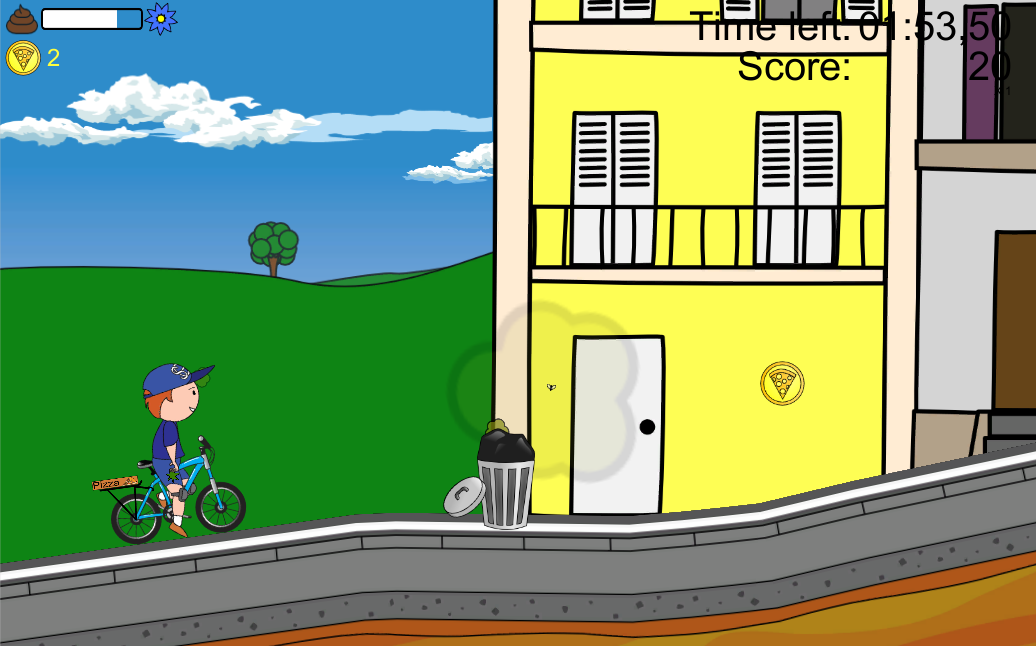
\includegraphics[height=\imgHeightMedium{}]{img/Analyse_BikeRehab2.PNG}}
				\captionof{figure}{Bike Rehab, jeu 2D demandant un exercice de pédalage.}
				\label{BikeRehab}
			\end{minipage}\medskip
						
			\item \textbf{Be The Ball --} Jeu de course où le patient influe sur la vitesse et la direction d'une boule sur un circuit dans un environnement en 3D (figure \ref{BeTheBall}). L'interaction se fait uniquement avec les jambes et s'inspire d'un exercice de \textit{press-leg}. La vitesse est influée par la pression effectuée (le robot reproduisant l'effet d'un ressort) et la direction par la différence de leur position. Un tableau des meilleurs scores par patient est effectué pour chaque niveau et le patient peut voir, durant la partie, une boule fantôme retraçant le parcours effectué par son meilleur score. Quatre niveaux sont disponibles: forêt; île; montagne; désert. Ces niveaux présentent chacun un environnement différent, plusieurs longueur sont représentées et certains tournent plus d'un côté et demande donc plus d'effort d'une jambe spécifique;\medskip
			
			\begin{minipage}{\linewidth}
				\makebox[\linewidth]{
					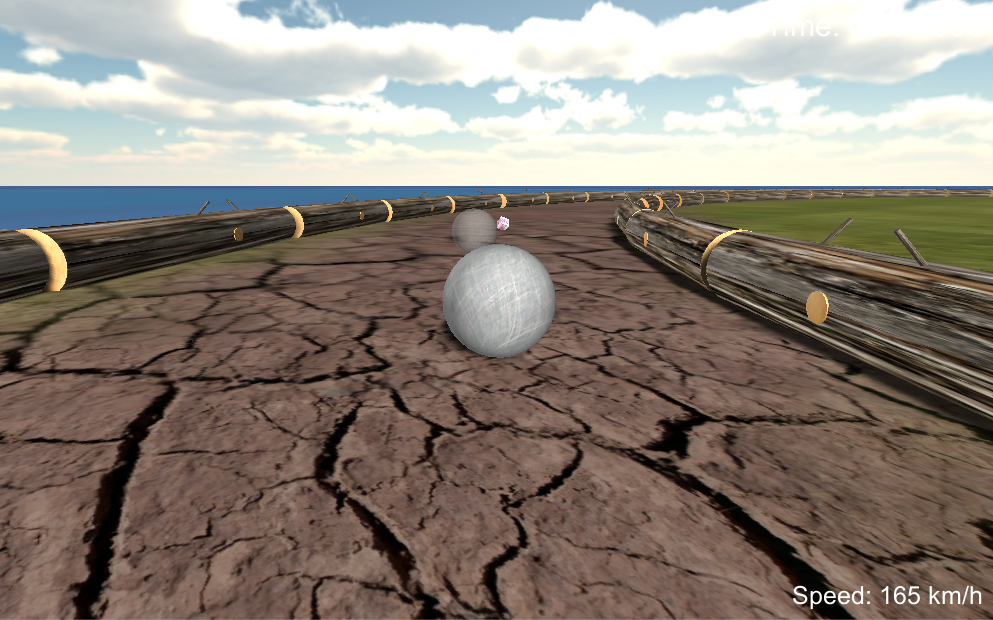
\includegraphics[height=\imgHeightMedium{}]{img/Analyse_BeTheBall2.PNG}}
				\captionof{figure}{BeTheBall, jeu de course demandant un exercice s'inspirant du \textit{press-leg}.}
				\label{BeTheBall}
			\end{minipage}\medskip
			
			\item \textbf{Gate Crossing --} Ce SG se déroule dans l'espace et demande également l'exécution d'un parcours bien définit. Alors que le SG précédent se basait sur une stimulation compétitive, celui-ci essaie de reproduire un environnement relaxant (environnement épuré et musique calme). La vitesse est constante et la direction est donnée par la différence de position entre les jambes (le robot n'applique pas de résistance supplémentaire). Le but étant de passer au centre de portes en faisant le plus de points (figure \ref{GateCrossing}). Contrairement au jeu précédent, on peut sortir du parcours et une redirection automatique est alors effectuée. Ce SG donne la possibilité d'utiliser le HMD mais peut être joué sur un écran également;\medskip
			
			\begin{minipage}{\linewidth}
				\makebox[\linewidth]{
					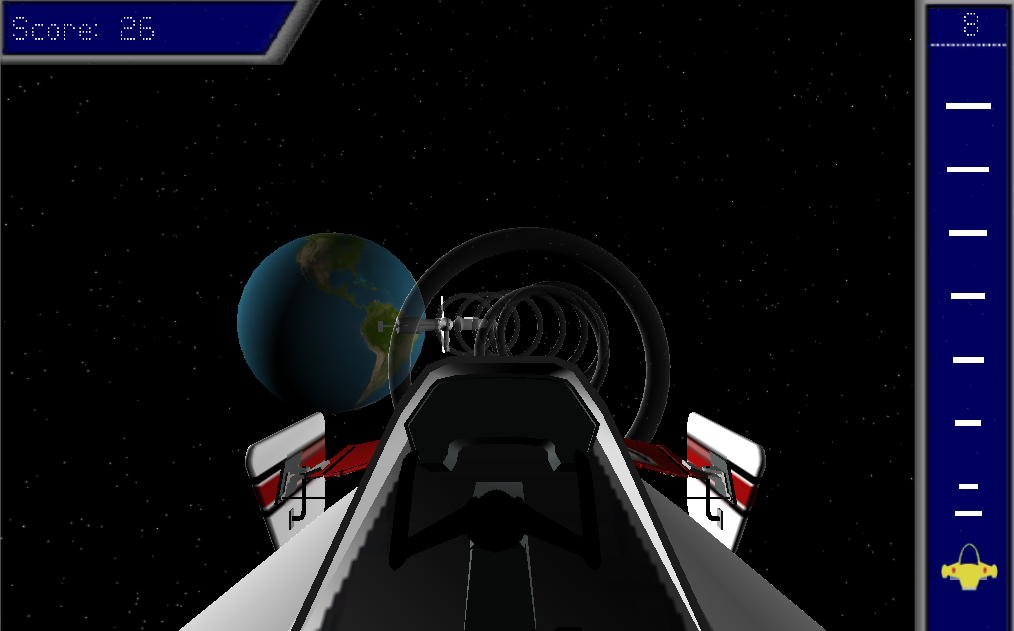
\includegraphics[height=\imgHeightMedium{}]{img/Analyse_GateCrossing2.PNG}}
				\captionof{figure}{Gate Crossing, jeu de précision demandant un exercice s'inspirant du \textit{press-leg}.}
				\label{GateCrossing}
			\end{minipage}\medskip
			
			\item \textbf{Pics Walk --} Ce SG a pour but de travailler la marche et oblige l'utilisation du HMD. Le patient doit donc reproduire un mouvement de marche (qui était simplifié par une ellipse dans un premier temps) avec la particularité de pouvoir réaliser ce mouvement de façon totalement passive. Une interaction supplémentaire était donc nécessaire pour créer une mécanique de jeu. Celle-ci est la prise de photos via contrôle vocal ou bouton (comme le saut de \textit{Bike Rehab}). Le patient peut donc, durant ses différents parcours, prendre certains éléments en photo (figure \ref{PicsWalk}). Quatre parcours dans deux environnements extérieurs différents évoquant la nature sont disponibles. En fonction de l'élément photographié, du cadrage (à l'aide du HMD), de la distance et d'autres facteurs, la photo rapporte certains points. Les photos peuvent être visionnées après une partie.\medskip
			
			\begin{minipage}{\linewidth}
				\makebox[\linewidth]{
					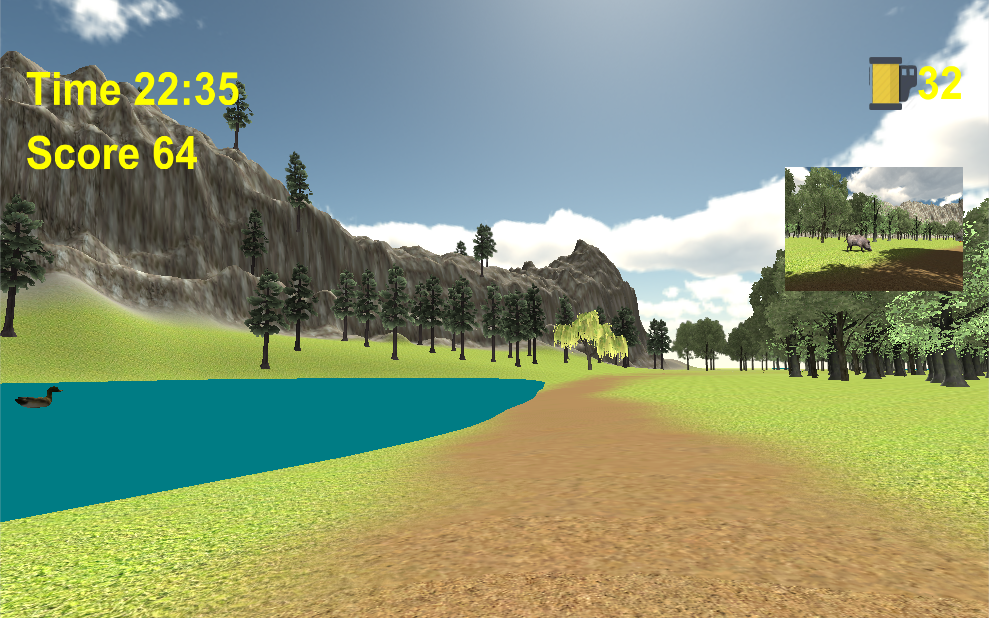
\includegraphics[height=\imgHeightMedium{}]{img/Analyse_PicsWalk2.PNG}}
				\captionof{figure}{Pics Walk, jeu d'exploration et de découverte demandant un exercice de marche.}
				\label{PicsWalk}
			\end{minipage}\medskip
		\end{itemize}		
	\end{itemize}

\section{Identification des objectifs}
	\label{sAnaDescriptionObjectifsCTI}
	Durant le projet R\&D, un seul SG devra être réalisé. Ses objectifs sont cités ci-dessous. À savoir que le SG conçu doit tenir compte de tous les objectifs, mais le délivrable implémenté lors de ce travail de Master ne couvrira qu'une sélection de ces objectifs (sélection effectuée dans la conception, section \ref{sConSelectionObjectifs}).
	
	\begin{itemize}	
		\item \textbf{Interfacés avec le LHS --} Le SG devra être interfacé et opérationnel avec le périphérique de réhabilitation LHS \cite{LHS_website}. Contrairement au projet SG4R, le SG n'aura pas besoin d'être interfaçable avec d'autres périphériques;
		
		\item \textbf{Jeu de marche --} Le SG doit demander au patient d'effectuer un mouvement de marche (qui est guidé ou accompagné par le LHS). Ce mouvement devra être répété longuement durant l'exercice et devra être perturbé le moins possible par d'autres actions. La durée d'un exercice est de 10 à 30 minutes, il faut donc s'assurer que le patient reste attentif et motivé durant toute cette durée;
		
		\item \textbf{Haute immersion --} Trois sens devront être sollicités par des stimuli de l'environnement virtuel. Si un stimulus doit affecter les trois sens, le patient doit les ressentir simultanément. Les sens sont: la vue; l'ouïe; le toucher. Pour la vue, le même HMD (\textit{Oculus Rift DK2} \cite{OculusDk2_website}) doit être utilisé. Il faut prendre garde à éliminer toute saccades du rendu visuel, afin que celui-ci soit fluide et paraisse naturel.
		
		Pour l'ouïe, une recherche d'ambiance sonore et de bruits (tels que les pas sur plusieurs types de terrains) devra être fait de façons approfondie.
		
		Pour le toucher, c'est le retour haptique du LHS qui sera utilisé. Il est souhaitable de simuler plusieurs types de terrains, des pentes ou encore des escaliers. Pour renforcer le toucher, on peut également, si l'on prend l'exemple de \textit{Pics Walk}, donner un appareil photo (ou un objet semblable) dans les mains du patient afin qu'il corresponde mieux à son avatar. Inversement, si le patient doit avoir un périphérique dans les mains, il est souhaitable que son avatar l'aie également;
		
		\item \textbf{Temps réel --} Le contexte d'exécution du SG contient plusieurs composants logiciels et matériels situés sur différents ordinateurs nécessitant de communiquer suite aux interactions de l'utilisateur afin de lui produire un retour (utilisant plusieurs modalités sensorielles). Ce retour doit être perçu comme instantané du point de vue du patient. Il faut donc faire attention à tout temps supplémentaire induit par le système et s'assurer que tous les composants soient synchronisés;
		
		\item \textbf{Représentation du mouvement --} Une représentation du mouvement que le patient effectue (qui est corrigé par le robot) devra être présente dans l'environnement afin d'augmenter le potentiel de la réhabilitation via l'activation des neurones miroirs. Les neurones miroirs sont des neurones qui s'activent à la fois lors de l'exécution d'un mouvement et durant l'observation du même effectué par une autre personne. Cette représentation pourrait donc être les jambes de l'avatar ou d'un autre personnage que l'on doit suivre;
		
		%TODO Peut être parler de ça (mais pas sûr: on ne justifie pas l'objectif qu'on a pas fixer nous...)
		%http://sergibermudez.blogspot.ch/2014/02/virtual-rehabilitation-beyond-gaming.html
		%et
		%"Often video games will include a representation of a player's limb(s) [15, 23, 74]. The use of a graphical representation of the upper extremitites builds on the paradigm of the motor neuron system as a method of augmenting neuroplasticity. Seminal research by neuroscientist Giacomo Rizzolatty prposed that the mirror neuron system activates in both goal-orientated action execution and action observation [101, 102]. Thus, the process of motor learning can occur as a result of watching, as well as physically performing, a movement. By including a virtual representation of a limb, it is hypothesized that the efficacy of a repetition-based exercise can be augmented with motor learning induced by the motor neuron system."
		
		\item \textbf{Niveaux d'appauvrissement et éléments familiers --} Certains patients peinent à interpréter une scène trop riche. %TODO Parler de l'exemple d'une salle de réveil en citant des sources (à faire probablement précédemment dans l'analyse) si documentation trouvée.
		Nos scènes devront pouvoir être affichées avec plusieurs niveaux d'appauvrissement en agissant notamment sur la complexité des éléments (structure, couleurs, animations, etc.) et leur nombre. Ces niveaux doivent prendre le moins de travail possible à être créés (éventuellement envisager des algorithmes les générant). Afin de rassurer le patient, certains éléments familiers (\textit{e.g.}, un cadre avec une photo) devront être présents. Cet aspect n'est pas apparu durant l'état de l'art ni l'analyse car il correspond à une demande directe du médecin collaborant avec le mandant. Demande issue de besoins constatés sur le terrain et n'ayant pas fait, à sa connaissance, l'objet d'études;%TODO: Nommer Rolf ?
		
		\item \textbf{Tests et validations --} Le SG devra être testé et validé par un certain nombre de personnes. Selon Jakob Nielsen une dizaine de personnes suffisent à trouver la quasi-totalité des problèmes. En voulant garantir qu'aucune latence n'est perceptible, 50 volontaires et 15 patients passeront un test. 50 personnes du domaine médical minimum testeront également le système afin de confirmer son objectif médical.
		
	\end{itemize}

\section{Contraintes et choix technologiques}
	\label{sAnaContraintes}
	Dans cette section sont résumés les différentes contraintes matérielles et logicielles concernant le SG à développer.
		\subsection*{Matériel} 
			\begin{itemize}
				\item \textbf{Robot Lambda --} Le robot de réhabilitation à utiliser développé par le mandant de ce projet. Il est composé de deux robots \textit{lambda} (figure \ref{Peripheriques}, image de gauche) un pour chaque jambe \cite{LHS_website}. Ils contiennent des moteurs pouvant assister, apporter de la résistance ou réaliser complètement les mouvements, ainsi que des capteurs de force dont les valeurs sont validées par des capteurs redondants. Les valeurs mesurées, ainsi que d'autres informations prétraitées peuvent être accédées par un logiciel tournant dans le noyau temps réel contrôlant le robot. Les informations prétraitées sont de plus haut niveau, tel que la position du pied, et sont obtenues à l'aide d'algorithmes complexes tenant compte de l'anatomie du patient. Ces informations doivent être utilisées comme une entrée du SG;	
				%TODO: Parler plus précisément des algo.
				
				\item \textbf{Oculus Rift DK2 --} L'utilisation du HMD est une des contraintes du jeu. L'\textit{Oculus Rift}, kit de développement 2 \cite{OculusDk2_website} (figure \ref{Peripheriques}, image de droite) étant actuellement en possession et utilisé par le mandant, il est à utiliser pour le SG. Ce HMD permet une vision stéréoscopique et des capteurs d'orientation permettent de savoir la direction dans laquelle le patient regarde. Des LEDs infrarouges sont également intégrées au casque et, à l'aide d'une caméra (livrée dans le kit de développement), permettent une localisation spatiale de la tête. L'utilisation de cette dernière n'est pas imposée. Elle nécessite une installation supplémentaire du LHS. À utiliser que si cela comporte un réel intérêt;
				
				\item \textbf{Microphone --} Les projets antérieurs se sont servi d'un micro pour certaines interactions à l'aide du contrôle vocal. Ceci vient d'une demande des médecins qui ont identifié le fait que certains patients peuvent présenter des difficultés à effectuer plusieurs actions en même temps. Ceci doit donc être réapprit et il est plus facile et utile de réapprendre à parler en marchant que de se servir d'un joystick. Ce mode d'interaction peut donc être réutilisé mais n'est pas une obligation;
				
				\item \textbf{Joystick --} L'utilisation d'un joystick, d'une manette de jeu ou d'une souris peut être envisageable. Attention cependant à ne pas le rendre obligatoire pour tous les stades de réhabilitation car certains patients n'arriveront pas à s'en servir;
				
				\item \textbf{PC SG --} Pour des raisons de performances et de facilité d'installation, le SG sera exécuté sur un ordinateur différent de celui de l'IHM et du noyau temps réel. Afin de ne pas complexifier la tâche du thérapeute, le PC ne disposera pas de souris ni de clavier et devra lancer le SG dès son démarrage. Le SG devra alors attendre la synchronisation et le signal de départ venant du LHS;
				
				\item \textbf{Casque audio ou haut-parleurs --} L'immersion devant utiliser le sens de l'ouïe, il est nécessaire d'avoir soit un casque audio, soit des haut-parleurs. Le premier ne concerne que le patient et permet une meilleure immersion s'il a une bonne isolation sonore. Si le thérapeute doit cependant communiquer avec le patient, ce dispositif est moins pratique. Des solutions de communication en jeu, via un micro ou des messages prédéfinis pourraient être envisageables. Ces messages font alors complètement parti de la réalité virtuelle où est le patient et peuvent provenir d'un autre personnage. Les haut-parleurs, de leur côté, imposent le son à tous les utilisateurs de la pièce et exposent le patient à des stimuli sonores hors de la réalité virtuelle dans laquelle il est immergé. Le thérapeute peut plus facilement communiquer avec le patient, cependant il y a de fortes chances que la présence du patient dans le jeu s'en voit impactée. \medskip
				
				\begin{minipage}{\linewidth}
					\makebox[\linewidth]{
						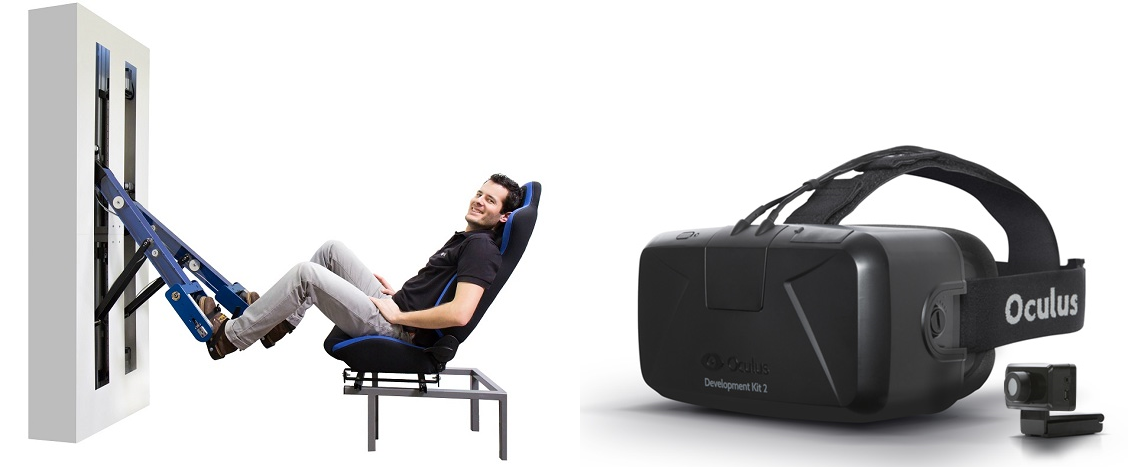
\includegraphics[height=\imgHeightSmall{}]{img/Peripheriques.png}}
					\captionof{figure}{Périphériques utilisés. Dans l'ordre de lecture: LHS; \textit{Oculus Rift}, kit de développement 2.}
					\label{Peripheriques}
				\end{minipage}\medskip	
			\end{itemize}
		\subsection*{Logiciels} 	
			\begin{itemize}
				\item \textbf{Unity \cite{Unity_website} --} Les SGs du projet SG4R ont été réalisés en utilisant le moteur de jeu Unity. Une version tout public gratuite contient l'intégralité du moteur de jeu et permet la création de jeux commercialisables. Ce produit n'est donc pas imposé mais fortement recommandé car il correspond aux attentes du mandant, a fait ses preuves dans les projets antérieurs et permettrait de faciliter la futur maintenance de l'ensemble des SGs. Son utilisation permet également de récupérer bien des éléments déjà développés dans les SGs précédents et ainsi mieux se concentrer sur les nouveaux aspects de ce SG. Pour ces raisons, il a été décidé de continuer à utiliser \textit{Unity} en écrivant les scripts en\textit{ C\#} \cite{CSharp_website};
				% Ayant participé aux projets antérieurs ainsi qu'au cours \textit{Game Technologies} du MSE qui a donné une formation sur ce moteur également, la prise en main sera facilité. Unity a été choisit (avec l'écriture des script en C\#).
				
				\item \textbf{Objectis Communication Foundation (Ocf) \cite{OcfClient_website} --} Cette technologie développée par Objectis \cite{Objectis_website} permet la simplification de la communication entre deux applications. Elle est imposée par le LHS car utilisée pour la communication entre les différents composants. Elle est donc à utiliser pour récupérer ou envoyer des données au LHS. Elle est basée sur une architecture client/serveur. Le serveur met à disposition une série d'objets que le client peut venir lire ou écrire de manière transparente.
				
				Dans le projet précédent, l'échange d'informations a été réalisé avec le protocole UDP et l'API d'Ocf \cite{OcfClient_website}. Cette dernière est écrite en \textit{C\#} \cite{CSharp_website} et utilise les types dynamiques présents uniquement depuis le \textit{framework} ".NET 4.0" \cite{DotNetFramework_website}.
				\textit{Unity} quant à lui utilise la version 2.0 de ce \textit{framework}, ce qui rend l'utilisation directe d'Ocf impossible depuis \textit{Unity}. La communication a alors été réalisée (pour le projet SG4R) via un programme supplémentaire. Celui-ci communiquant avec le jeu via mémoire partagée. L'utilisation d'Ocf est donc obligatoire et la mémoire partagée est fortement recommandée.
			\end{itemize}		
		
		\subsection*{Contextuels}
			Le patient jouera aux SGs à l'hôpital (ou en clinique) car le LHS ne prévoit pas (pour le moment) une utilisation à domicile. Cela implique quelques contraintes contextuelles qui influent sur la conception du SG.
			\begin{itemize}
				\item \textbf{Fréquence des sessions --} La fréquence des sessions de réhabilitation est de une à cinq par semaine. Elles durent une heure, mais il ne faut compter que 10 à 15 minutes de SG. De plus, le SG ne sera pas obligatoirement utilisé à chaque session. On peut donc mettre en place un mécanisme de récompense (et non de punition) hebdomadaire;
				\item \textbf{Présence du thérapeute --} Le thérapeute est présent tout au long de l'exercice. C'est lui qui doit choisir l'exercice ainsi que ses paramètres. Il doit pouvoir modifier la difficulté si besoin. Le LHS avec son IHM possède déjà une interface convenant aux thérapeutes pour régler et agir sur un exercice. Si le SG doit contenir des réglages (paramètres de difficulté, choix du niveau, etc.) et des retours supplémentaires pour les thérapeutes (\textit{e.g.}, score "héminégligence"), ils doivent être disponibles via cette interface. Ces interfaces devront être le plus simple d'utilisation et d'interprétation possible.
			\end{itemize}		
	
\section{Éléments pour la conception d'un SG de neuroréhabilitation}
	\label{sAnaGameConceptPointsImportant}
	Dans cette section sont détaillés tous les éléments à prendre en compte pour la conception d'un jeu d'après la documentation trouvée. L'accent est mis sur les implications et concrétisations des objectifs listés précédemment.
	\begin{itemize}
		\item \textbf{Présence et immersion --} D'après Witmer et Singer REF, quatre facteurs clés détermine la présence \cite{Witmer_MeasuringPresence}:
		\begin{enumerate}
			\item \textbf{Facteur sensoriel --} La figure \ref{5Senses} représente la qualité de l'immersion et la difficulté de rendu d'une réalité virtuelle pour chaque sens ajouté (somme cumulée). On remarque que dès l'ajout du touché, on obtient une immersion presque totale.
			
			\begin{minipage}{\linewidth}
				\makebox[\linewidth]{
					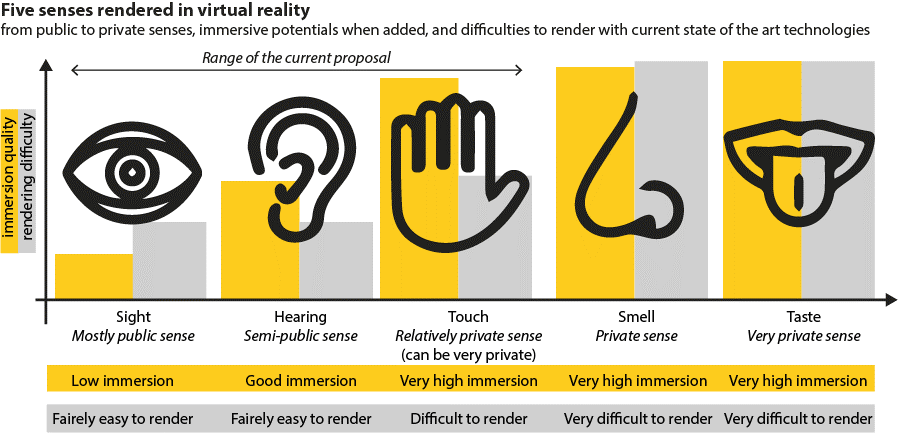
\includegraphics[height=\imgHeightMedium{}]{img/Analyse_5SensesInVR.png}}
				\captionof{figure}{Difficulté d'implémentation et renforcement de la présence pour les cinq sens en réalité virtuelle.}
				\label{5Senses}
			\end{minipage}\medskip
			
			À noter que le facteur sensoriel ne dépend pas uniquement de la présence de stimuli pour les sens souhaités mais également de leur qualité.
			
			Pour ce projet, les sens ciblés sont la vue, l'ouïe et le toucher. La vue est stimulée à l'aide du HMD. L'ouïe à l'aide d'un casque audio ou d'haut-parleurs. Le touché via le retour haptique du robot qui devra donner aux jambes l'impression réelle de l'action qui est en train d'être effectuée (\textit{e.g.}, type de terrain, pente, escalier);
			
			\item \textbf{Facteur de contrôle --} Plus le patient a un sentiment de contrôle, plus sa présence sera renforcée. Ce sentiment de contrôle est basé sur les interactions que le joueur peut avoir avec son environnement afin qu'il se sente acteur et non spectateur.	
			En plus des interactions, il faut que le \textit{game flow} soit bon. Ce dernier étant bon si l'équilibre entre le challenge demandé et les capacités de la personne est respecté (plus de détails sur sa définition et ses implications décrit au point suivant). Trop de challenge induirait de l'anxiété et trop peu de l'ennui. Si ce \textit{game flow} est bon, le patient aura alors un sentiment de contrôle et sa présence sera renforcée;
			
			\item \textbf{Facteur de distraction --} Les distractions liées à l'environnement réel du joueur doivent être réduites au minimum. En utilisant un HMD et un casque audio avec une forte isolation, on peut ainsi garantir que tous les stimuli visuels et sonores viennent de l'environnement virtuel et non de l'environnement réel. Attention, cela peut, dans notre cas, être contraire au besoin qu'a le thérapeute de communiquer avec le patient. Pour maximiser la présence du joueur mais tout de même permettre au thérapeute de communiquer avec le patient, il est possible de placer un autre agent dans l'environnement qui donnerait les instructions que le thérapeute dicte (au micro ou à l'aide de messages préenregistrés).			
			L'interface du jeu et les différents retours d'informations ne doivent pas non plus distraire le joueur;
			
			\item \textbf{Facteur de réalisme --} Le réalisme ne comprend pas uniquement de beaux graphismes, mais une cohérence entre les différents éléments de la scène (\textit{e.g.}, source de lumière et ombre). Chacune de ces incohérences peut alors diminuer la présence de l'utilisateur. Il est important de se souvenir de ce point durant le développement, cependant, la plupart de ces détails seront réglés par le moteur de jeu lui-même. À nous, par contre, de trouver des éléments étant cohérents placés ensemble dans la même scène (style graphique).
		\end{enumerate}
		
		\item \textbf{Game flow - expérience optimale --} Le \textit{game flow} est le ressentit de l'utilisateur sur le challenge que le jeu demande. Le sentiment d'avoir le contrôle sur le jeu \cite{Salen_RulesOfPlay}. Il est bon si l'équilibre entre le challenge demandé et les capacités de la personne est respecté. Trop de challenge induirait de l'anxiété et trop peu de l'ennui. Le niveau optimal ce situe lorsque la tâche est difficile mais faisable \cite{Green_ExercisingBrain}. C'est dans cet équilibre que le joueur aura une expérience optimale du jeu.
		\\
		
		Une des techniques utilisée pour maintenir un bon \textit{game flow} est l'ajustement automatique de la difficulté \cite{Alankus_TowardsCustomizableGames, Cameirao_RehabilitationGamingSystem, Burke_DesigningEngagingPlayableGames4Rehab}. Le challenge augmente plus le joueur réussi et diminue quand il échoue (figure \ref{DifficultyAdjustment}). Une évaluation faîte par Burke et al. \cite{Burke_DesigningEngagingPlayableGames4Rehab} a montré un intérêt des joueurs à ce système d'équilibrage, même pour des personnes saines (80\% ont remarqué cet ajustement et l'ont apprécié). Attention cependant à ce que cet équilibrage ne soit pas trop brusque et que la difficulté n'augmente pas trop rapidement dès que le patient réussi. L'analyse de l'augmentation et de la diminution de ces facteurs permet également une étude plus approfondie des capacités de l'utilisateur au long d'une session d'exercices. Il est possible de proposer des niveaux de difficulté (facile, intermédiaire, expert) contenant tous un ajustement automatique de la difficulté mais variant le seuil de réussite ou d'échec avant de modifier les paramètres. Si la difficulté ne réside pas dans l'exécution du mouvement de réhabilitation (comme les SGs "Bike Rehab" et "Pics Walk" du projet SG4R), il est envisageable de laisser l'utilisateur la régler. En lui montrant l'influence de chaque paramètre sur la récompense finale, il pourra alors essayer des réglages plus dur pour gagner plus. L'utilisateur fixant son propre but a alors plus de contrôle et peut augmenter sa motivation \cite{Nagle_DifferentDifficultyAdaptation}.
		
		\begin{minipage}{\linewidth}
			\makebox[\linewidth]{
				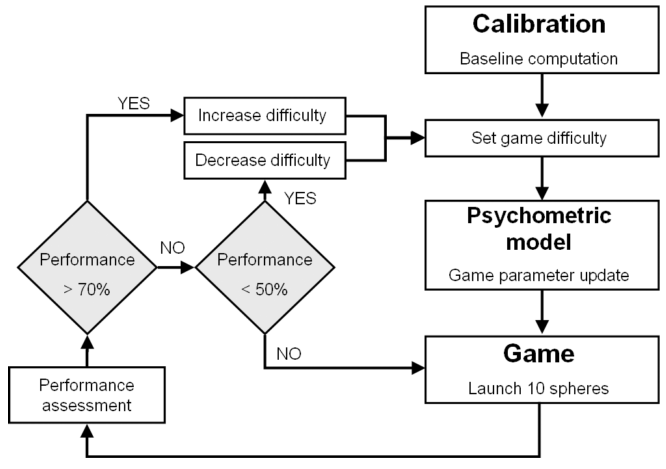
\includegraphics[height=\imgHeightMedium{}]{img/Analyse_Cameirao_DifficultyAdjustment.PNG}}
			\captionof{figure}{Diagramme d'ajustement automatique proposé par Cameirão et al. \cite{Cameirao_RehabilitationGamingSystem}.}
			\label{DifficultyAdjustment}
		\end{minipage}\medskip
		
		Les paramètres souvent utilisés dans les SGs pour la réhabilitation sont: la taille, la vitesse et le lieu des différents objectifs. Ces paramètres, avant de s'ajouter automatiquement, doivent être initialisés manuellement ou par une calibration. Dans tous les cas, le thérapeute doit pouvoir modifier ces paramètres. En modifiant ces paramètres il peut également être possible de travailler différents aspects d'un objectif tels que la vitesse ou la précision \cite{Alankus_TowardsCustomizableGames}.
		
		Dans un jeu habituel, la gestion de la difficulté est souvent en lien avec le nombre d'échec que va subir le joueur. Dans un SG de réhabilitation, l'échec doit être traité avec précaution. Trop d'échec pourrait rapidement être lié à une perte d'engagement car le patient l'associe directement à ses propres capacités motrices et physiques. C'est pourquoi Burke et al. \cite{Burke_DesigningEngagingPlayableGames4Rehab} recommandent d'aborder cet échec de façon encourageante (\textit{e.g.}, ne pas dire "Vous êtes mort. Réessayer ?" mais plutôt "Félicitations, vous avez obtenu 150 points.");
		
		\item \textbf{Environnement virtuel --} Une étude a été menée sur 14 participants pour savoir si un environnement virtuel naturel induisait plus de relaxation et moins d'anxiété qu'un environnement virtuel urbain. Cette étude se fit en deux étapes. La première montrait simplement l'environnement sur un écran. Le résultat montra une faible préférence pour l'environnement naturel mais pas de manière significative. La deuxième étude montra qu'en ajoutant une ambiance sonore, l'anxiété augmenta et la relaxation diminua dans l'environnement urbain alors que l'inverse a été observé dans l'environnement naturel \cite{VARSG4HC1}.
		Un dernier aspect notable est que, d'après Alankus et al. \cite{Alankus_TowardsCustomizableGames}, si l'environnement contient des personnages non joueur, il serait souhaitable de pouvoir interagir avec eux;	
		
		\item \textbf{Temps réel --} Afin de garantir que le SG puisse être considéré comme une application temps réel, on doit s'assurer que les différents retours utilisateur soit générés dans un maximum de temps donné, ne provoquant ainsi pas de perception de latence et n'augmentant pas le taux d'erreur de l'utilisateur. Une étude \cite{Jay_RT_ModelingEffectsDelayedHaptic} a montré que s'il fallait 50 ms de latence (temps entre l'interaction et le retour d'information) visuelle pour qu'une personne la remarque (pouvant provoquer des \textit{Breaks In Presence}), il en faut 25 de moins pour l'haptique. En effet, à plus de 25 ms, la latence n'est pas forcément perceptible, cependant le taux d'erreur de l'action augmente. Pour garantir la cohérence lors de la réhabilitation, il faut donc que l'haptique et les autres modalités soient à moins de 25 ms de latence. Autrement dit, chaque action que l'utilisateur effectue doit avoir déclenché des retours dans les modalités souhaitées en moins de 25 ms;
		
		\item \textbf{Progression --} D'après Dennis W. Fell  \cite{Fell_ProgressingTherapeuticInvervention}, la progression est un élément clé de l'apprentissage moteur. Elle doit se faire durant une session mais également sur l'ensemble de la réhabilitation. Cette progression peut se concrétiser avec l'augmentation du niveau de difficulté. Cette progression à court et long terme doit également être visible par le patient afin d'augmenter son engagement \cite{Burke_DesigningEngagingPlayableGames4Rehab};
		
		%TODO: Parler des courbes d'évolution de difficulté
		
		\item \textbf{Principe de l'apprentissage moteur --} Pour qu'un SG soit efficace dans le cadre d'une réhabilitation, il doit comprendre des instructions, des \textit{feedbacks} et un agenda d'entraînements appropriés \cite{SGVW_EducationProfDevHealthCare}. Il doit également présenter des informations individualisées pour différents types d'individus et différents stades d'apprentissage. Le livre donne également quatre points pour un apprentissage qui se fait de façon transparente:
		\begin{itemize}
			\item \textbf{Adaptativité --} Donner des astuces ou retour d'informations adaptables au patient, ou encore lui adapter son environnement;
			\item \textbf{Adaptation et personnalisation --} Constitutionnelle, qui s'adapte aux dimensions d'une personne et autres contraintes physiques. D'après les préférences et capacités cognitives de l'utilisateur. Physiologique, qui agit en cours de partie, d'après les capacités physiques actuelles du patient mais également sur le long terme, entre plusieurs sessions;
			\item \textbf{\textit{Game mastering} --} Le jeu ne peut pas tout savoir. Il faut quelqu'un qui connaisse bien le jeu et le but pour pouvoir évaluer au mieux les performances et donner de bons retours (dans notre cas: les thérapeutes);
			\item \textbf{Reconnaissance d'activité et détection d'erreur --} Reconnaître le mouvement que le patient est en train d'effectuer et pouvoir mesurer un degré de réussite ou d'échec.
		\end{itemize}
		
		\item \textbf{Addiction --} Comme dans la plupart des jeux actuels, l'identification et l'achèvement d'objectifs permet de stimuler la compétitivité d'un joueur et de maintenir son engagement.
		%TODO: Approffondir après avoir lu le livre.
		%"Modern video games aim to engage the user in extended periods of play whereby large volumes of repetitive button presses are required to complete on-screen objectives. The mechanisms which mediate the upkeep of this behavior are a complex and diverging multidisciplinary study in itself [105].
		
		Les récompenses sont un moyen de maintenir l'engagement du joueur. Cependant si celles-ci sont trop régulières elles finissent par le lasser. Induire un aléa dans la distribution de récompenses ou la baser sur des paramètres variables permet de maintenir une plus grande motivation. Cette attribution des récompenses peut être basée sur des préférences utilisateur, certains nécessitant plus d'encouragements que d'autres \cite{Nagle_PlayerCenteredRewardScheduling};
		
		\item \textbf{Feedback --} D'après Dennis W. Fell \cite{Fell_ProgressingTherapeuticInvervention} les feedback sont un élément clé de l'apprentissage moteur et doivent être nombreux au début afin que le patient puisse se corriger et progresser. Cependant, plus le patient progresse, plus les feedbacks doivent diminuer laissant ainsi de l'autonomie au patient;
		%TODO: En parlé quand les full-texte sont reçu (demande envoyé sur la plateforme de recherche).
		%"Feedback is the mediator between the system and player, and is known to be an important motivator for motor learning [2]." 
		
		\item \textbf{Interactions --} Alankus et al. ont publié un article \cite{Alankus_TowardsCustomizableGames} partageant leurs expériences acquises durant le développement de SGs pour patient atteint d'un AVC. Voici de leurs recommandations, celles pertinentes dans notre cas pour les interactions.
			
		Premièrement, pour permettre aux patients présentant différents niveaux de réhabilitation de jouer au SG, il est souhaitable de pouvoir utiliser plusieurs périphériques d'entrée.	Deuxièmement, le public cible pouvant présenter des troubles cognitifs et n'étant pas obligatoirement habitué aux jeux vidéo, les interactions doivent être les plus naturelles possibles. Pour finir, il est tout de même souhaitable de donner la possibilité de réaliser des interactions complexes demandant la coordination de plusieurs actions pour progresser dans la réhabilitation des tâches de tous les jours. Ainsi, plusieurs interactions évoluant au cours de la réhabilitation seraient souhaitables. 
		
		Si l'interaction que l'utilisateur réalise est liée à un mouvement physique, il existe également des lois décrivant la vitesse attendue d'après certains facteurs. La loi de Fitts semble adéquate pour régler la difficulté via la vitesse pour un jeu de réhabilitation du bras. \cite{Zimmerli_ValidationBalanceDifficulty}.
	\end{itemize}	
		
		
	\chapter{Conception}
		Dans ce chapitre (section \ref{sConGameConcept}), la conception du SG est décrite telle qu'il devrait être d'après la description du projet R\&D. Cette conception cherche à répondre à tous les objectifs identifiés précédemment dans l'Analyse (section \ref{sAnaDescriptionObjectifsCTI}) et à être compatible avec le plus de points importants mis en avant (section \ref{sAnaGameConceptPointsImportant}). L'ensemble de ces objectifs et donc du SG conçu n'est pas implémenté dans ce travail, une sélection est faîte et détaillée dans la section \ref{sConSelectionObjectifs}. Les principaux risques concernant l'implémentation de cette sélection d'objectifs sont ensuite décrits dans la section \ref{sConIdentificationRisques}. Les approches permettant de minimiser leurs probabilité d'apparition ainsi que leurs impacts y sont décrites également. Ce chapitre se conclut par une description de la communication conçue (section \ref{sConCommunication}).

\section {Concept du jeu}
	\label{sConGameConcept}
	Le concept global du jeu est l'exploration de planètes à la recherche de traces d'une civilisation disparue. Ce concept permet de correspondre aux objectifs du projet R\&D (section \ref{sAnaDescriptionObjectifsCTI}) mais également aux points importants à prendre en compte lors de la conception d'un tel SG (section \ref{sAnaGameConceptPointsImportant}). Il a été élaboré avec le Prof. Dr. Stéphane Gobron (professeur d'infographie, responsable de l'ancien projet SG4R et du projet à venir) de la HES-SO Neuchâtel et le Prof. Dr. Michel Lauria (responsable des équations de mouvements du projet SG4R et du projet à venir) de la HES-SO Genève. Ce concept a ensuite été validé par le mandant. Celui-ci ainsi que ses possibilités sont présentés en détails dans les sous-sections à venir.
	
	\subsection*{Histoire du jeu}	
		Après de nombreuses années de voyage, le vaisseau d'exploration arrive dans une galaxie avec de nombreuses planètes qui offraient ou semble offrir les conditions idéales pour le développement d'une civilisation. C'est au joueur d'explorer ces planètes afin de trouver des traces de cette civilisation. Le but étant de découvrir ce qu'elle est devenue.
		Le voyage spatial ayant duré de nombreuses années, les membres de l'équipage ont les muscles atrophiés et sont obligés d'explorer les planètes en commençant par celles ayant peu de gravité.
	
	\subsection*{Élémentss différentiateur}		
		Comparé aux autres SGs développés pour le LHS, celui-ci propose un scénario et une grande possibilité d'amélioration. De plus, les paramètres thérapeutiques tels que l'assistance, la gravité ou l'appauvrissement de la scène ont un sens dans le scénario (\textit{e.g.}, constante de gravité de la planète pour l'assistance du robot). De plus, ce SG peut poser une base pour de futurs, ou dores et déjà existant, SG pouvant être liés tout en proposant d'autres exercices et ainsi, à long terme, rejoindre l'idée de plateforme (utilisation de véhicule pour du pédalage ou encore session de vol pour rejoindre le vaisseau, ce qui peut correspondre au SG \textit{SpaceGate}).
	
	\subsection*{Environnement virtuel}
		L'environnement est composé de l'intérieur du vaisseau spatial ainsi que la surface des différentes planètes à explorer.
		
		L'intérieur du vaisseau spatial est une zone contenant des objets familiers (table, chaise, cadre, etc.). Elle sert également de zone de transfert entre la salle où se trouve le patient et une réalité virtuelle sur une planète inconnue. Cette zone doit être neutre et pouvoir ressembler à une salle d'hôpital. Le patient devra la traverser en marchant afin d'en sortir, offrant ainsi une transition entre les deux types d'environnement et inversement. Le joueur s'y trouve donc au début et à la fin de chaque session de jeu.
		
		Les planètes peuvent, elles, être très différentes. Composées de terrains désertiques contenant seulement des rochers, peu de couleurs (mars) et aucun voire peu de sons, comme celle maquettée en figure \ref{Maquette}. À l'inverse, ce peut être une planète contenant beaucoup d'êtres vivants tels que des arbres et des animaux, très riche en couleurs, formes et sons. L'appauvrissement ou l'enrichissement de tels mondes inconnus peut être plus cohérent que s'il s'agissait d'endroit connus. 
		
		Le SG contient différents types de sols avec différentes textures, effets sonores et sensations haptiques. Il peut également contenir des pentes et marches. La présence de points d'eau (changeant le coefficient de viscosité) peut permettre une immersion progressive.\medskip			
		
		%TODO: Uniformiser couleurs, tailles et polices des légendes
		\begin{minipage}{\linewidth}
			\makebox[\linewidth]{
				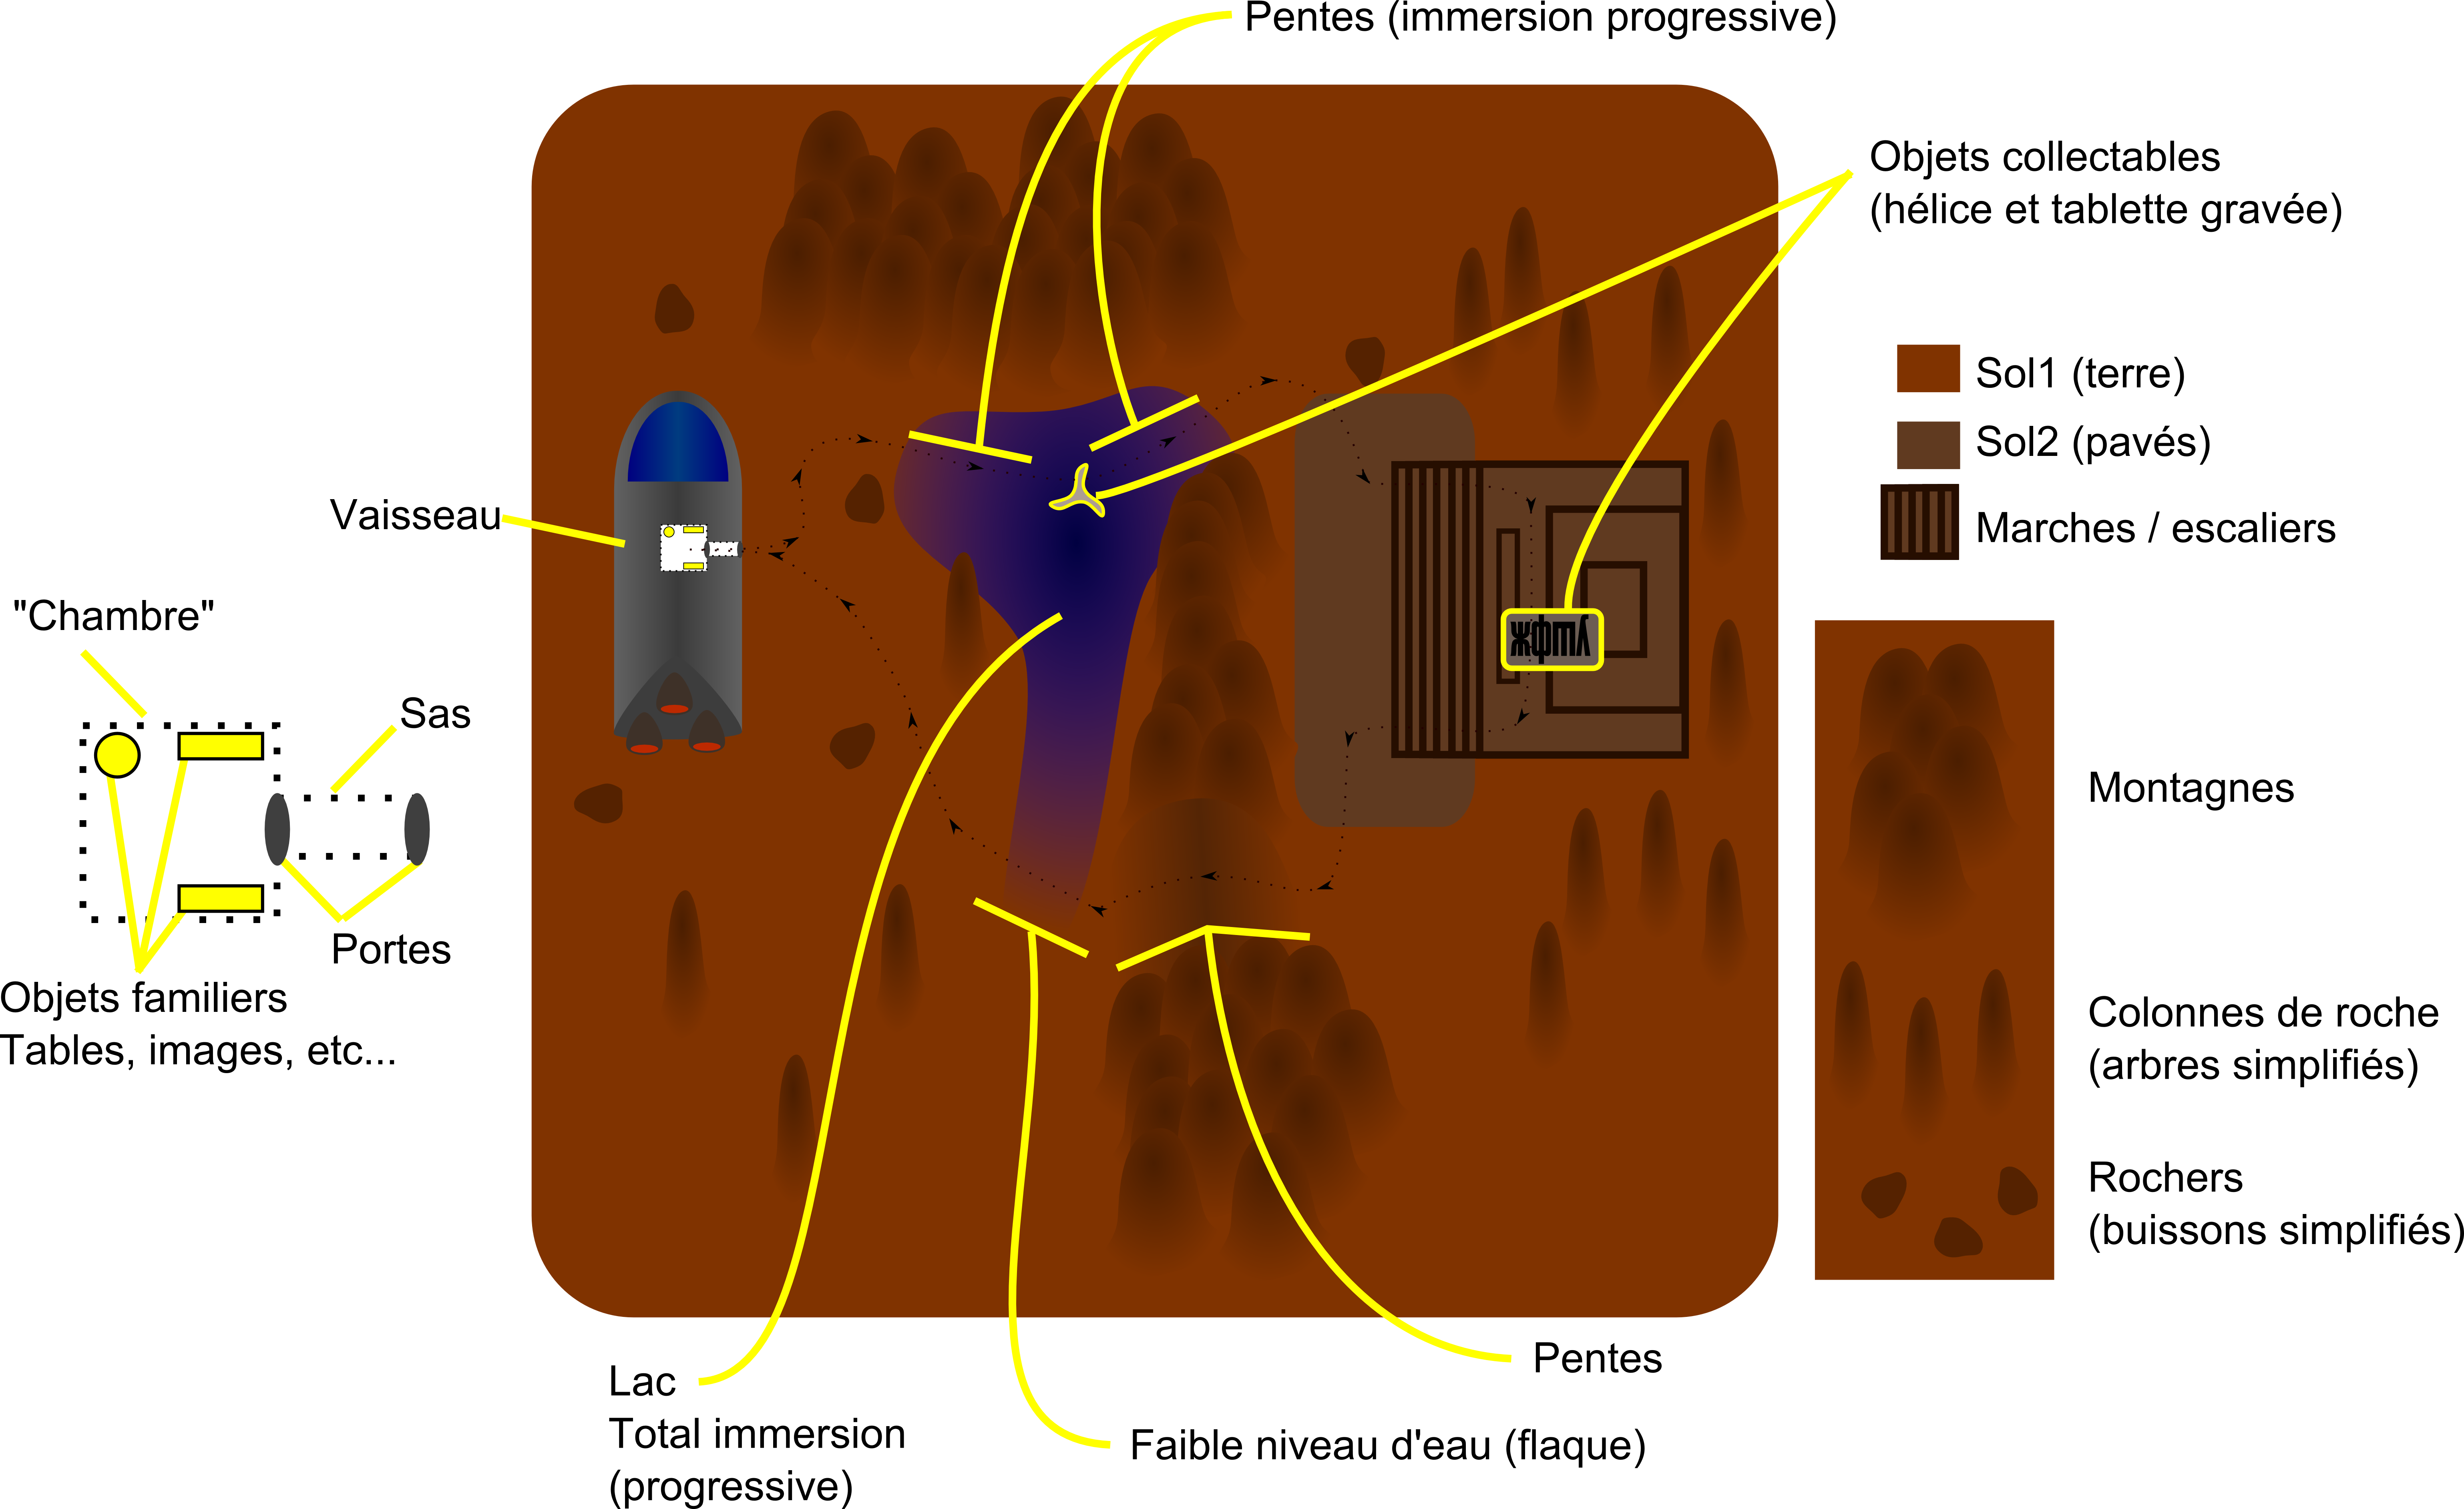
\includegraphics[width=\textwidth]{img/Conception_MaquetteAvecLegende.png}}
			\captionof{figure}{Maquette de l'environnement du jeu avec le parcours et les éléments à trouver.}
			\label{Maquette}
		\end{minipage}\medskip		
		
	\subsection*{Gameplay}
		Une session de jeu effectue un niveau qui consiste en une "sortie" sur une planète. Celle-ci suit un parcours bien défini que le joueur ne peut modifier. Le but étant de trouver et collecter des indices sur cette civilisation. Les mécanismes de recherche et de collecte pourront évoluer au cours de la réhabilitation (cf. sous-section suivante). Les deux principaux arguments ayant menés à la décision d'un chemin défini sont les suivants: simplicité d'interaction et simplicité des modèles mathématiques. Un déplacement libre aurait implicitement dû ajouter un moyen de tourner et, par conséquent, une interaction supplémentaire, ce qui n'est pas souhaitable. L'hypothèse d'effectuer la rotation par rapport au regard est exclue car ce n'est pas une façon naturelle de se déplacer (et aurait donc put nuire à la neuroréhabilitation) et cela interfère avec toutes autres interactions de recherche dans l'environnement (primordiale pour trouver les traces de la civilisation). L'autre raison (simplicité des modèles mathématiques) provient des contraintes pour la modélisation mathématique du mouvement en tenant compte du type de sol. La complexité est nettement diminuée si, dès l'initialisation du SG, les modèles peuvent connaître toutes les pentes et types de sols du parcours. Dans le cas contraire, même durant le projet R\&D, ce modèle ne pourrait être implémenté.
		\\
		
		Le challenge du jeu est alors de collecter suffisamment d'indices lors d'une sortie pour pouvoir passer au point d'exploration suivant (ailleurs sur la planète ou sur une autre). Le nombre d'indices peut être indiqué à l'avance (\textit{e.g.}, "Six artéfacts correspondant à la signature fréquentielle de la civilisation ont étés détectés"). Des indicateurs peuvent être mis en place si le joueur effectue plusieurs fois la même sortie sans trouver d'indices (\textit{e.g.}, "Des scans approfondis ont permis de localiser plus précisément les artéfacts"). Si ce challenge est jugé insuffisant, un score ou une appréciation peuvent être réalisés par la suite en fonction du nombre d'objectifs trouvés, l'aide nécessaire, l'énergie dépensée, l'état de la combinaison spatiale, etc. Bien que certains de ces éléments soient dépendants d'interactions spécifiques n'intervenant pas en début de thérapie.	
		\\
		
		On peut également imaginer une progression faisant corréler l'avancement du SG avec une réhabilitation cognitive. Le patient commencerait par des planètes "désertiques" et, au fur et à mesure de sa réhabilitation, découvrirait des planètes plus riches (abandonnées depuis moins longtemps). Ce schéma de progression est cependant grandement lié au profil des patients (certains n'auront aucun troubles cognitifs alors que d'autres pourront peut-être réapprendre à marcher mais uniquement dans des endroits appauvris). Afin de ne pas se restreindre à un profil précis et de permettre la progression du SG et de la réhabilitation motrice à la plus grande plage de patients, aucune progression de ce style ne doit être présente. Il pourrait cependant être intéressant de voir s'il est possible d'établir des profils de patients et ainsi de proposer une progression en relation.
		
	\subsection*{Personnages et contrôles}
		Le joueur contrôle un avatar à la première personne. Toutes les parties se font avec un autre personnage non joueur que l'on devra suivre. Celui-ci effectue un mouvement de marche correcte et sert à l'activation des neurones miroirs mais peut également être la représentation du thérapeute, lui donnant des conseils dans sa réhabilitation. La principale interaction étant donc la marche via le LHS pour faire avancer l'avatar, les rotations devant être légères et automatiques (parcours défini et non libre). Des obstacles à éviter (flaque / cailloux) pourront être utilisés pour rendre le patient plus conscient de ses mouvements si cela est souhaitable par les thérapeutes. Cela ne rentre cependant pas dans le cadre du premier produit à réaliser. Les sorties auront un temps défini (durée de l'exercice) lié à l'oxygène de la combinaison spatiale. En conséquent, les pauses durant l'exercice doivent être évitées.
		
		La façon dont les indices sont recherchés et collectés peut évoluer au long de la réhabilitation pour correspondre au besoin d'ajout d'interactions (voir analyse, section \ref{sAnaGameConceptPointsImportant}). Par exemple, au début, l'autre personnage peut réussir à découvrir quelques indices, le joueur doit juste le suivre. Par la suite, le joueur peut indiquer les objets à collecter en les fixant du regard (HMD). Ensuite il pourrait les collecter ou prendre des photos d'éléments intéressants via contrôle vocal/simple bouton. Finalement, d'autres interactions peuvent être mises en place telles qu'un zoom, une détection radar, etc.
		
	\subsection*{Choix techniques}
		Pour les raisons détaillées dans l'analyse (section \ref{sAnaContraintes}), le SG sera développé avec \textit{Unity} avec des scripts en \textit{C\#}. Les modèles 3D devront être trouvés sur internet. %TODO: Dire que c'est pas justifier/raisonnable de passet 1j à la création d'un truc alors qu'un designer le fait en une heure ?
		L'avatar (ses jambes) devra être animé d'après les angles et positions des segments corporels calculés par le LHS. Les différentes modalités de retour devront être garanties à une fréquence où aucun délai n'est perceptible par l'utilisateur (détaillé dans l'analyse, section \ref{sAnaGameConceptPointsImportant}).
		Le SG tournera sur un PC dédié et communiquera avec le noyau temps réel ainsi que de l'IHM. Le PC ne contiendra qu'un écran, un \textit{Oculus Rift} et d'éventuels autres périphériques pour le SG (micro, bouton, manette de jeux, etc.). Il devra se lancer automatiquement et contenir un minimum de paramètres ou interfaces accessibles au patient pour démarrer la partie au plus vite.
		

\section{Sélection des objectifs}
\label{sConSelectionObjectifs}
	Dans cette section sont repris tous les objectifs du projet R\&D décrits dans l'analyse, section \ref{sAnaDescriptionObjectifsCTI}. Ils sont triés par ordre de priorité décroissant. Chaque sous-section décrit ce que le SG à développer durant ce travail doit contenir et ce qui est laissé au projet suivant (le SG devant faciliter leur future intégration).
	\subsection*{Niveaux d'appauvrissement}
		Pour les niveaux d'appauvrissement, il est décidé de pouvoir travailler sur différents aspects: densité des objets; modélisation géométrique; audio; rendu des couleurs; animations; effets de lumière. Le SG fournit donc plusieurs variables pouvant être modifiées à souhait et offre ainsi de nombreuses combinaisons possibles. Par la suite, pour simplifier la configuration, le thérapeute n'aurait accès qu'à une variable "Appauvrissement" et chaque aspect serait définit d'après sa valeur. Cela nécessite d'avoir des retours du domaine médical sur cet appauvrissement. Il est décidé que ces retours s'obtiendraient après ce travail, en présentant le SG implémenté.
		
		Ci-dessous, est présenté de façon approfondie chacun de ces aspects ainsi que des solutions techniques pour les réaliser. Afin de tester la faisabilité de certains, des tests ont été effectués avant la phase de développement. Les tests et leurs conclusions présentent cependant un aspect plus technique et sont donc expliqués dans le chapitre développement, section \ref{sDevAppauvrissement}.
		\begin{itemize}
			\item \textbf{Densité des objets --} Paramètre influant sur la quantité des objets de la scène allant de zéro à un. "Zéro" correspondant à aucun objet et "un" à la scène comme elle censée être pour un patient ne souffrant d'aucun trouble cognitif. Seuls les objets de décors, tels que des arbres ou cailloux sont influencés. Les objets à trouver, quant à eux, seront toujours présents. Ce paramètre influe donc légèrement sur la difficulté du jeu, moins il y aura d'autres objets, plus il sera facile de trouver les traces de la civilisation. Cet appauvrissement fait partie des objectifs du SG réalisé durant la phase de développement;
			
			\item \textbf{Modélisation géométrique --} Ce paramètre influe la modélisation géométrique des objets de décors. Il peut modifier la complexité de celle-ci en utilisant d'autres techniques (\textit{e.g.}, \textit{billboard}) ou simplifier celle qui est actuellement utilisée en diminuant, par exemple, le nombre de détails ou de sommets du modèle à l'aide d'une application tierce. Le SG doit donc proposer ces différentes modélisations géométriques pour chaque objet de décor;
			%TODO: étoffer.
			
			\item \textbf{Audio --} Ce paramètre influe sur la richesse des effets sonores. Plusieurs possibilités sont identifiées et le choix de celle retenue dépend des fichiers audio trouvés (la création des fichiers sonores n'entrant pas dans les tâches de ce projet, ils doivent être trouvés sur internet).
			
			La première, s'adaptant principalement aux musiques, consisterait en un appauvrissement "par instrument" des sons. Cela nécessite de trouver des fichiers sonores contenant plusieurs pistes pour chaque instrument.
			
			La deuxième possibilité consiste pour chaque son de trouver différentes pistes audio de plusieurs sources mais devant représenter le même son avec une complexité différente. Cette possibilité nécessite une grande recherche de fichiers sonores et nécessite de définir la notion de complexité (notes, instruments, durée, etc.) de façon plus précise pour être cohérente pour tous les différents sons. Un autre problème est qu'il est difficile de trouver des fichiers correspondant au même composant sonore du jeu, se ressemblant mais de complexité différente. Ce problème peut s'illustrer avec la musique de fond: à moins d'utiliser une musique connue et donc disponible avec de multiples interprétations, ce sera une musique certes d'une autre complexité mais différente pour chaque niveau d'appauvrissement ce qui retire de la cohérence au SG. La solution semblant être la plus réalisable consiste à trouver des sons correspondant au niveau le plus riche, puis de modifier ces musiques (logiciels tiers ou algorithme de traitement de signal) pour en proposer des versions appauvries.
			
			La dernière possibilité est probablement la plus simple car elle ne nécessite qu'un fichier audio par son (facilement trouvable sur internet) et aucun traitement. Elle consiste à proposer pour chaque son deux valeurs: actif et inactif. En classant les sons par famille (bruit d'ambiance, musique de fond, son d'interface, etc.) on peut alors choisir quels types de sons sont actifs et cela offre de nombreuses combinaisons possibles pour l'appauvrissement sonore.
			
			Le choix et l'implémentation d'une de ces techniques d'appauvrissement fait partie des objectifs du SG réalisé durant la phase de développement;
			
			\item \textbf{Nombre de couleurs --} Ce paramètre doit influer le nombre de couleurs présentes dans la scène. Plusieurs possibilités sont réalisables pour la sélection de ces couleurs (palette de couleurs, diminution du nombre de valeurs possibles des composantes, etc.);
			
			\item \textbf{Animation --} Certains éléments de décors peuvent avoir des animations ou des effets de particules. Le SG réalisé durant la phase de développement doit alors proposer le choix de les activer ou non;
			
			\item \textbf{Effets de lumière --} Pour les effets de lumières, trois valeurs doivent être disponibles dans le SG développé: uni; diffus; diffus et spéculaire. Pour le niveau "uni", la valeur est la même pour toutes les parties de l'objet (comme si l'on utilisait une lumière ambiante). Pour "diffus", on obtient un dégradé en fonction de l'orientation de la surface avec la lumière (objet mat). Les effets spéculaires du dernier point correspondent aux reflets de la source de lumière (surface brillante).
			%TODO: Trouver et placer une image illustrant les 3 (idéalement, du livre de STG).
			
		\end{itemize}
	
	\subsection*{Représentation du mouvement}
		Le jeu doit contenir deux représentations d'un mouvement de marche. La première est celle du mouvement que le patient effectue qui est reproduit sur les jambes de son avatar. Les angles des différentes articulations calculés par l'application temps réel du LHS doivent être reportés sur cet avatar et son état doit correspondre à celui du joueur sans pouvoir percevoir de décalage temporel. Le joueur peut jouer assis ou allongé et l'angle entre son dos les jambes au repos peut varier. L'avatar doit quant à lui rester debout et maintenir cet angle fixe. Ainsi, en baissant la tête, le patient pourra analyser son mouvement en temps réel.
		
		La deuxième représentation est celle du guide que le joueur doit suivre. Le guide devra rester à une distance suffisante pour analyser son mouvement. On ne doit pas pouvoir le dépasser et il doit nous attendre. Le mouvement que le guide effectue peut être une animation de marche allant avec le modèle 3D ou trouvée sur internet.
		
		Le guide et le joueur doivent avoir un déplacement dans le monde correspondant à l'amplitude de leurs pas et ainsi éviter un effet de glisse sur le sol. Des modèles mathématiques seront développés durant le projet R\&D pour obtenir le déplacement exact. Pour ce travail de Master, il faut simplement veiller à limiter cet effet de glisse et trouver une technique temporaire de déplacement convaincante sans pour autant se soucier de son exactitude.
		
		Un autre point souhaitable, afin de tenter de mieux activer les neurones miroirs, serait que le guide ai un mouvement de marche correct mais synchronisé avec celui du patient. Une option permettant un aperçu de notre mouvement (pouvant être activé par le thérapeute) est également souhaitable. Les deux options de ce paragraphe sont cependant hors de ce travail de Master.
	
	\subsection*{Jeu de marche}
		Le jeu doit contenir au minimum deux mondes différents. Les parcours doivent boucler afin de commencer et finir dans le vaisseau spatial. L'un des niveaux doit tourner sur la droite et l'autre sur la gauche afin de ne pas défavoriser des patients souffrant d'héminégligence.
		Si, suite aux premières démonstrations, cette boucle est jugée problématique par le domaine médical, il est possible de faire des niveaux droit où, une fois sorti du vaisseau, ce dernier décolle et vole jusqu'au point d'arrivée du parcours où il atterrit et nous attend. Cela est cependant hors des objectifs de ce projet.
		Le parcours doit avoir des virages les plus doux possibles pour éviter les effets de nausée. En effet, le joueur étant guidé sur le chemin, ce n'est donc pas lui qui choisit de tourner ou qui tourne réellement, il ne fait que subir. Cette différence peut provoquer des nausées si elle est trop importante.		
		Ce parcours n'a pas à contenir de pente. Pouvoir gravir ou descendre des pentes, avec un retour haptique adéquat, est un des objectifs du projet R\&D mais ne peut être implémenté que durant celui-ci et non ce travail de Master.
		L'implémentation et la gestion des mondes doit faciliter l'intégration de nouveaux mondes générés d'après des critères tels que le temps de marche et d'autres liés à la pente. Cependant, pour ce projet, ces mondes peuvent être entièrement réalisés à la main et n'ont pas à correspondre à ces contraintes.
		\\
		
		Concernant l'interaction, il est expliqué dans l'analyse (section \ref{sAnaGameConceptPointsImportant}) que proposer plusieurs interactions pouvant être changées durant la réhabilitation est un point important. Cependant seule une de ces interactions doit être implémentée pour ce projet. Elle doit correspondre à la première interaction qu'un patient aurait à faire, la plus intuitive.
		\\
		
		Le scénario, la mise en situation du joueur ainsi que d'autres aides, sont à transmettre au joueur sous forme de dialogues audio. Ceux-ci n'ont pas à être réalisés durant ce travail. Le SG produit doit tout de même permettre la visualisation d'une certaine progression, même si le scénario n'est pas expliqué.
	
	\subsection*{Haute immersion}
		Comme expliqué dans la description des objectifs R\&D dans l'analyse (section\ref{sAnaDescriptionObjectifsCTI}), le SG doit utiliser des modalités de retour dans les sens de la vue, de l'ouïe et du touché. Pour la vue, le SG développé doit utiliser un HMD et ne doit pas percevoir de saccade. Pour l'ouïe, des musiques et des sources sonores placées dans la scène en trois dimensions doivent être utilisées. Combiné avec un casque audio stéréo et le HMD, le joueur pourra alors localiser la source dans son environnement. Le projet R\&D pourra couvrir des aspects plus avancés utilisant des casques audio pouvant rendre un son en trois dimensions, cependant cela va au-delà de ce travail de Master.
		\\
		
		Le dernier sens est le toucher qui est stimulé à l'aide du retour haptique. Il est ainsi possible de donner la sensation de différents types de sols ou milieux dans lesquels le joueur évolue. Cet aspect nécessite cependant un grand travail dans l'application gérant le robot LHS. Cet aspect ne pourra être traité que durant le projet R\&D et sort des objectifs de ce travail de Master.
		
		Les différents aspects de sols doivent tout de même être perceptibles visuellement en utilisant différentes textures et auditivement avec plusieurs types de bruits de pas.
		
	\subsection*{Interfacé avec le LHS}
		Le SG développé doit être interfacé avec le LHS. Une session d'exercice doit pouvoir être lancée depuis l'IHM. Le SG doit tenir compte des différents états du LHS et récupérer l'état du patient (calculé par l'application temps réel du LHS d'après la position du robot et la force des capteurs). Les détails des informations échangées est décrit dans la section \ref{sConCommunication}.
	
	\subsection*{Éléments familiers}
		Toutes les sessions de jeu devront commencer et finir à l'intérieur du vaisseau spatial. Cette zone de commencement doit être neutre et devra, d'un point de vue contenu et textures, être plus proche d'une salle d'hôpital que celle d'un vaisseau spatial, afin d'offrir une transition plus douce au patient. Cette salle doit contenir des éléments familiers au joueur tel que des meubles, un cadre ou encore une photo. La possibilité d'y intégrer des objets personnels du patient (tel qu'une photo de sa famille, ou encore un objet important) serait également intéressant mais sort des objectifs de ce travail de Master.
	
	\subsection*{Temps réel}
		La garantie de temps réel (50 ms maximum) est un point important. Le SG développés dans ce travail devra mesurer ces performances et, si elles sont à améliorer, identifier de potentielles causes. La résolution de celles-ci sort des objectifs de ce travail.
	
	\subsection*{Tests et validations}
		Des tests validant l'utilité du SG nécessite l'avis de plusieurs personnes du domaine médicale, voire même la réalisation de tests cliniques. Ceci ne doit pas être fait durant ce travail. Il est cependant attendu que le SG soit testé par une personne du domaine médicale afin d'obtenir des premiers retours et d'identifier ses perspectives futures.

\section{Identification des risques}
	\label{sConIdentificationRisques}
	Dans cette section sont analysés les différents risques potentiels qui pourraient nuire au bon déroulement du projet ainsi que le moyen de minimiser leur probabilité d'apparition et leur impact. Ces risques sont listés en sous-section dans l'ordre décroissant de leur probabilité.
	
	\subsection*{Situation temporelle du travail}%TODO Voir pour supprimer cette sous-section pour éviter de se "tirer un balle dans le pied"
		Comme expliqué dans l'analyse (section \ref{sAnaEtatDesLieux}), ce travail n'est qu'une sous partie d'un projet R\&D impliquant de nombreux intervenants. Ce dernier ne pourra pas démarrer avant la fin de ce travail. Il en va de même de la disponibilité des intervenants du projet R\&D. Le risque est alors présent que le SG nécessite des éléments ne pouvant être développés que bien plus tard (tels que le retour haptique ou le mouvement de marche). Ce point est déjà pris en compte dans la sélection des objectifs (\ref{sConSelectionObjectifs}) où tous retours haptiques sont exclus de ce travail.
		
		%Ce risque est également présent dans les relations avec le mandant devant effectuer quelques taches de développements pour intégrer le SG et dont l'aide est nécessaire pour implémenter la communication et tester le SG dans une situation d'utilisation proche de la réalité.
		Afin de minimiser l'impact, il faudra réaliser des simulateurs fonctionnant par exemple sur une interaction clavier. Ces simulateurs doivent permettre, entre autre, de vérifier que le mouvement des jambes soit correct. Cependant, le mouvement de marche est complexe et sa modélisation ne doit pas être produite dans ce travail. Le mouvement simulé peut alors être une approximation permettant de tester le SG sans correspondre exactement à un mouvement correct.
		
		%Ce risque est également présent avec les partenaires du monde médicales devant intervenir dans le projet R\&D. Sachant que leur disponibilité sera faible, il faudrait idéalement avoir un contact en début de projet pour identifier notamment les points important de l'appauvrissement de la scène et effectuée une démonstration en fin pour avoir leur avis final. Obtenir leur feedback tout au long du projet et des versions du SG de façon plus agile serait idéale mais pourrait ne pas être réalisable.
		
	\subsection*{Interaction de deux mondes, ingénierie et médial}
		%Comme décrit dans la sous-section précédente, la collaboration avec le domaine médicale risque d'être faible. Ceci implique le risque que le produit développé ne corresponde que partiellement aux attentes de ce domaine.
		Les domaines de l'ingénierie et du médical sont différents et l'interaction entre eux peut s'avérer difficile. %TODO: Reformuler et mieux introduire
		Afin de minimiser l'impact d'éventuelles mécompréhensions, il faut veiller à ce que le SG soit bien structuré et permette la suppression de fonctionnalités ou l'ajout de nouvelles avec facilité. Pour cela, il faut minimiser le couplage entre les scripts et le respect du patron "Modèle-vue-contrôleur" (MVC) est décidé.
		\\
		
		Les fonctionnalités non sûres, telle que le comportement de l'appauvrissement de la scène, devront tout de même être implémentées mais avec un accent plus prononcé sur le nombre, leur possibilité, leur présentation plutôt que leur niveau de finition. Attention également à la compréhension entre le monde médical et celui de l'ingénierie: un aspect pouvant être considéré comme un détail de finition pourrait être vu comme un  problème important par le domaine médical. Il faut alors essayer d'anticiper ces points et de préparer des démonstrations sur la facilité de changement.
		Les principaux aspects du SG étant impactés par ce risque sont:
		\begin{itemize}
			\item \textbf{Appauvrissement de la scène --} Ce point vient d'être expliqué dans la description de ce risque. Pour minimiser l'impact de mauvaises interprétation, il faut mettre l'accent sur le nombre d'aspects pouvant être appauvrit et leur démonstrations plutôt que sur la finesse de cet appauvrissement. Ces aspects d'appauvrissement doivent montrer le plus de possibilités réalisables;
			\item \textbf{Éléments familiers --} Il est décidé dans la sélection des objectifs (section \ref{sConSelectionObjectifs}) que ce point ne concerne que l'intérieur du vaisseau et ne consiste qu'en une pièce neutre composée d'éléments familiers tels que table, cadre, etc. Toute autre possibilité est sortie des objectifs de ce projet. L'impact de ce risque sur ce point est donc minime;
			\item \textbf{Environnement virtuel --} Les différents mondes crées peuvent ne pas correspondre aux attentes des thérapeutes ou contenir des aspects qu'ils identifieraient comme pouvant poser des problèmes aux patients. Pour minimiser la probabilité d'apparition de ce risque, il est souhaitable de créer des mondes proches d'un environnement terrestre et peu fantaisistes. Le contexte de l'espace et de planètes inconnues pourrait être déduit par la présence d'astres dans le ciel ou d'éléments de décors particuliers sans forcément avoir un environnement trop étranger. Pour minimiser l'impact de ce problème, il est souhaitable de pouvoir aisément changer les mondes ou en créer de nouveaux.
			%\item \textbf{Mouvement de marche --} Il est possible que le mouvement de marche de l'avatar ou du guide ne convienne pas aux thérapeutes. La réalisation d'un mouvement de marche correct n'entre pas dans les objectifs de ce travail. Le mouvement de l'avataur doit simplement 
		\end{itemize}
	\subsection*{Fichiers ressources du SG}
		Le SG doit utiliser de nombreuses ressources (\textit{assets}) tels que des fichiers sonores, des modèles 3D, des textures, etc. La plupart de ces fichiers doivent être trouvés sur internet car leur réalisation impliquerait les compétences d'un \textit{designer}. Ce sont les modèles 3D qui souffrent du plus de contraintes pour le SG. D'abord, il faut trouver des modèles correspondant aux objets souhaités, puis s'assurer que cette modélisation corresponde à tous nos critères. Exemples de critères: la cohérence des styles entre les différents modèles; le droit d'utilisation; le nombre de sommets (influant sur les performances du SG); les besoins en animation (pour l'avatar ou le vaisseau spatial).
		\\
		
		Pour minimiser l'impact de ce risque, il est souhaitable de choisir un style graphique neutre (réaliste) où l'on trouvera probablement le plus grand nombre d'éléments cohérents ensembles. En l'absence d'éléments parfaits, il est souhaitable d'utiliser ceux correspondant aux plus de critères, donnant ainsi un aperçu de ce que le SG peut donner. Ces éléments pourront par la suite être modifiés, refait ou achetés s'ils donnent déjà un aperçu concluant du SG.
	\subsection*{Temps réel}
		Ne pas pouvoir respecter les contraintes temps réel est un risque. Ceci peut provenir de deux sources: le calcul et l'affichage du SG et la communication avec le LHS.
		Pour l'affichage, le principal risque est de surcharger la carte graphique avec des composants trop lourds. Ce point, en relation directe avec le nombre de sommets des modèles 3D, est hautement lié avec la sous-section précédente. Il se traduit par un effet de saccades ou de désynchronisation entre les yeux visibles dans le HMD, surtout lors de mouvements rapides de la tête. Pour minimiser sa probabilité d'apparition, il faut veiller à utiliser en quantité raisonnables des modèles avec peu de sommets et éviter un affichage dupliqué sur l'écran et le HMD. Pour minimiser son impact, il faut veiller à faciliter le remplacement des objets (\textit{e.g.}, en automatisant les étapes générant les géométries appauvries).
		\\
			
		Pour la communication, les SGs précédent étaient capable de garantir le temps réel. Ceci avec des entrées provenant d'un autre ordinateur, une communication utilisant Ocf \cite{OcfClient_website} (API de communication à utiliser, expliqué dans la section \ref{sAnaContraintes}) et effectuée par un tiers programme, communiquant au SG par mémoire partagée. Il existe tout de même un risque que cette communication dans ce nouvel SG ne puisse répondre aux contraintes temps réel car, comme il est expliqué dans la section \ref{sConCommunication}, aucun de ces prédécesseurs ne récupérait autant de donnée et Ocf  \cite{OcfClient_website} semble effectuer une requête par valeur. Pour contourner ce problème s'il se présente, il faudra récupérer une variable composée (tableau ou objet) contenant toutes celles utiles (tâches d'implémentation impliquant des modifications du logiciel gérant le LHS ce qui rejoint le premier risque cité).
			
	%\subsection*{Perception du SG}
		%Le SG n'as pas pour but d'isoler le patient et de supprimer le thérapeute. Il ne doit pas être perçu ainsi.	
	
	%TODO: Faire une matrice probabilité d'apparition x impact ?
		
\section{Communication avec le LHS}
	\label{sConCommunication}
	Dans cette section est détaillé l'ensemble des entrées et sorties (I/O) nécessaires au SG, une description de la machine d'état du LHS ainsi qu'une description de la gestion de ces I/O.
	
	\subsection*{Entrées/sorties (I/O)}
		Pour remplir les objectifs définis, le SG n'a besoin de communiquer que le message de fin de jeu à l'IHM. Ce message est la seule sortie actuelle du SG et est transmis quand le patient a atteint la fin du niveau. Le LHS ne mémorisant pour le moment aucune information liée aux sessions de SG, un booléen est suffisant pour cette information. Par la suite, le SG devra également communiquer la pente ainsi que le type de sol. Comme expliqué dans la description du \textit{Gameplay} (section \ref{sConGameConcept}), chaque niveau propose un parcours fixe. Pour simplifier les modèles mathématiques (et les rendre réalisables dans le projet R\&D), le SG devra communiquer, dès le chargement du niveau, les hauteurs et les types de sols de l'ensemble du niveau. Seul l'avancement du joueur sur ce parcours sera alors communiqué à chaque instant du SG. Cela sort cependant des objectifs du SG développé dans ce travail de Master.
		\\
		
		Les entrées du jeu sont nombreuses. Le SG doit, à chaque instant, connaître pour chaque jambe l'angle de chaque segment (hanche, genou, cheville), si le pied touche le sol, ainsi que l'ange d'inclinaison du siège. Ce dernier ne changeant pas durant l'exercice, il peut être récupéré uniquement à l'initialisation. Les plages exactes des mesures sont présentées de façons plus détaillées dans la section \ref{sDevArticulation} du chapitre "Développement".
		Pour savoir si le pied touche le sol, les modèles mathématiques seront utiles. Puisque ceux-ci ne seront pas implémentés durant ce travail, une solution temporaire devra être trouvée (idéalement du côté LHS).
		Le SG doit également connaître l'état du LHS pour savoir quand lancer la partie, l'arrêter ou encore si le thérapeute a mis pause à l'exercice. Les différents états du LHS nous concernant sont expliqués dans la sous-section suivante.
		
		Cela représente donc les variables suivantes. Six nombres réels de type \textit{float}, trois par jambe. Deux booléens, un par jambe. Un entier de type \textit{int}, état du LHS. Elles sont à lire pour calculer chaque état du SG. Un \textit{float}, correspondant à l'inclinaison du dos est également à récupérer en début de partie.
		
	\subsection*{Machine d'état}
		Sur les différents états du LHS, seuls trois nous intéressent:
		\begin{itemize}
			\item \textbf{RunExercise --} L'exercice est lancé et le patient peut interagir avec le robot pour effectuer le mouvement. Le SG doit attendre que le LHS soit dans cet état pour commencer le décompte du temps;
			\item \textbf{StopExerciseState --} Le LHS est dans cet état quand le thérapeute interrompt l'exercice manuellement. Le SG doit alors s'arrêter en indiquant les scores du patient;
			\item \textbf{PauseExercise --} Le LHS est dans cet état quand le thérapeute met l'exercice manuellement en pause. Le SG ne doit alors plus compter le temps qui s'écoule et bloquer les différentes interactions. Pour des raisons d'immersion, le patient doit toujours pouvoir regarder autour de lui (mais plus effectuer de \textit{scan}).
		\end{itemize}
	
	\subsection*{Gestion des entrées/sorties (I/O)}
		La figure \ref{DeploymentClassDiagram} montre les différents composants du système, leurs communications ainsi que la technologie utilisée pour celles-ci. Comme expliqué dans l'analyse (section \ref{sAnaContraintes}), on ne peut utiliser directement depuis \textit{Unity} l'API Ocf \cite{OcfClient_website} qui est nécessaire pour communiquer avec l'application temps réel. La raison de ce problème est que l'utilisation de types dynamiques dans Ocf n'est pas présent dans la version du \textit{framework} ".Net" utilisée par \textit{Unity}. Cette communication se fait alors via un programme à développer. La communication entre ce programme et notre SG se fait alors par mémoire partagée (déjà utilisée dans le projet SG4R car jugée comme l'alternative la plus rapide et régulière \cite{ZanniniRapport}).
		\medskip			
		
		\begin{minipage}{\linewidth}
			\makebox[\linewidth]{
				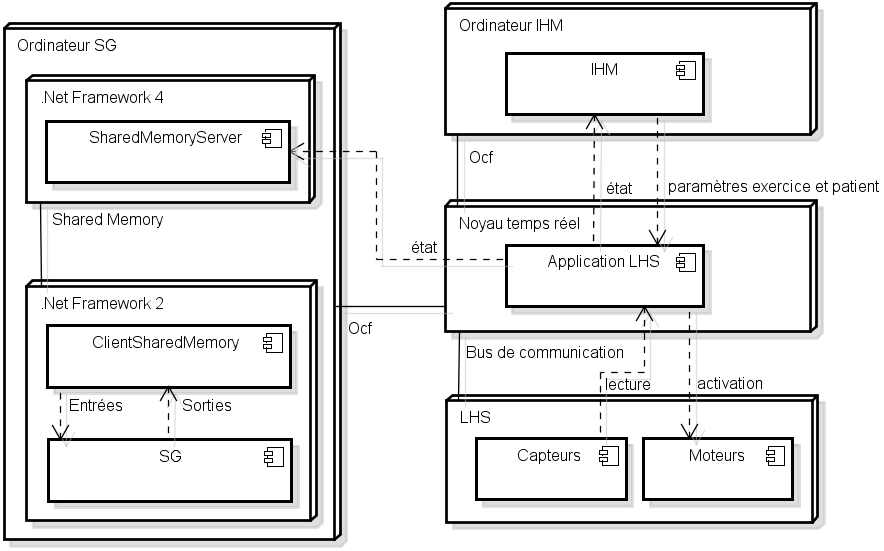
\includegraphics[width=\textwidth]{img/Conception_CommunicationDeploymentDiagram_Resized.png}}
			\captionof{figure}{Diagramme de déploiement montrant les différents composants et leurs interactions.}
			\label{DeploymentClassDiagram}
		\end{minipage}\medskip%TODO: En annexes, voir laisser une miniature ici aussi
				
		Cette structure nécessite donc l'implémentation d'un programme agissant en tant que serveur pour la mémoire partagée, d'une API agissant en tant que client et d'une librairie contenant les classes communes à s'échanger. Un diagramme de classe (présent dans les annexes) montre cette structure ainsi que l'abstraction du contrôleur d'entrées/sorties qui permettra la création d'un simulateur afin de tester le SG sans le LHS.
		
		Afin de garantir le temps réel, le serveur ne se contente pas de récupérer les valeurs quand on le lui demande. Dans un \textit{thread} supplémentaire, il récupère constamment les valeurs présentes dans l'application temps réel et les met à disposition du client. Le client lit ces dernières valeurs et aucune attente n'est effectuée sur une requête réseau. Cette solution, bien qu'elle ne garantisse pas le temps réel de l'interaction, peut utiliser d'anciennes valeurs si les requêtes Ocf ne sont pas terminées \cite{ZanniniRapport}.
		
	\chapter{Développement logiciel}		
		Ce chapitre détaille le développement des différents aspects du SG. Une vision globale de l'ensemble du SG, est disponible dans le chapitre "Résultats", à la section \ref{sResActualSG}.  Premièrement, afin d'avoir une vue d'ensemble, sa structure est détaillée sous plusieurs aspects dans la section \ref{sDevStructure}. Ceci afin d'avoir une idée sur la façon dont le projet est exécuté, construit et implémenté. Ensuite, les détails sur l'implémentation des principales fonctionnalités du SG (d'après les objectifs) sont décrits en trois autres sous-sections. La section \ref{sDevAppauvrissement}, décrit en détail le système d'appauvrissement actuel mais également tous les tests ayant été réalisés pour y arriver. La section \ref{sDevDeroulementPartie} décrit différents éléments liées à l'aspect "jeu" du SG et décrit également le déroulement d'une partie. La dernière, section \ref{sDevArticulation}, parle de la présence des différents mouvements de marche dans le SG et de l'articulation de l'avatar.
\\

Sur la fin du développement, Monsieur Kevin Laipe, un stagiaire du groupe imagerie de la HE-Arc a été mis à contribution pour ce projet. Sous ma supervision, il a réalisé principalement des tâches de design pour enrichir quantitativement le SG. Sur la fin, le développement de certaines fonctionnalités lui ont été assignées. Son aide a permis d'étoffer le contenu du SG, d'identifier les différents \textit{bugs} grâce à de nombreux tests et de tester l'architecture du SG. L'ajout de niveaux et fonctionnalités a permis de tester le faible couplage des fonctionnalités existantes et la facilité d'ajout de contenu. Les éléments réalisés par Monsieur K. Laipe sont les mondes supplémentaires (de deux à cinq), l'appauvrissement des animations, l'ajout du son de scintillement aux objectifs, la scène utilitaire "ObjectiveViewGenerator" et les images des objectifs utilisées dans le choix des niveaux.%TODO: Éviter la formulation "MON encadrement"

\section{Structure du projet}
	\label{sDevStructure}
	Dans cette section est décrite, sous plusieurs aspects, la structure du projet. La langue choisie pour nommer les différents éléments développés est l'anglais. Les exemples de cette section ont donc des noms anglais.
	\subsection*{Structure du projet et environnement}
	La communication et les différentes entités nécessaires à l'exécution du projet sont implémentées comme elles ont été conçues (section \ref{sConCommunication}). Comme dans le précédent projet, le programme tiers faisant le lien entre Ocf et la mémoire partagée met constamment à jour ses valeurs afin de garantir le temps réel. Trois projets C\# \cite{CSharp_website} ont été réalisés pour implémenter cette communication:
	\begin{itemize}
		\item \textbf{ClientSharedMemoryLibrary --} Ce projet crée une libraire "ClientSharedMemoryLibrary.dll" en \textit{.NET} 3.5 pour pouvoir utiliser la mémoire partagée. Bien que Unity supporte officiellement \textit{.NET} 2.0, certains aspects de la version 3.5 sont utilisables (tels que la mémoire partagée) \cite{UnityDotNETVersion};
		\item \textbf{ServerSharedMemoryProcess --} Ce projet crée un exécutable en \textit{.NET} 4.5 (pour l'utilisation de types dynamiques). Celui-ci récupère, à son lancement, les paramètres initiaux (l'inclinaison du siège). Puis, en boucle, dans un \textit{thread} séparé, les dernières valeurs de l'application temps réel à l'aide d'Ocf. Il les place ensuite dans la mémoire partagée pour être accessible au client;
		\item \textbf{SGData --} Ce projet crée une librairie "SGData.dll" \textit{.NET} 3.5 contenant toutes les classes passées dans la mémoire partagée.
	\end{itemize}
	Le client de la mémoire partagée peut réaliser trois actions: demander les paramètres initiaux; demander les dernières valeurs; fermer la mémoire partagée. C'est quand il demande les dernières valeurs qu'il indique si le jeu est terminé ou non. Cette information est ensuite transmise à l'application temps réel qui termine l'exercice. L'exercice peut également être terminé par le thérapeute, depuis l'IHM. Dans ce cas, le SG le saura en récupérant les dernières valeurs (l'état du LHS sera "StopExerciseState", voir section \ref{sConCommunication}).	
	%TODO: Parler d'un ordre de lancement
	
	La persistance du projet se fait actuellement en local sur l'ordinateur exécutant les SG. Seul un fichier, nommé "save.dat" est créé et il se trouve dans le dossier "\%AppData\%/LocalLow/HEArc/SGTM". Le SG ne tient pas compte de plusieurs utilisateurs. La principale raison étant que l'identification du patient n'est pas possible à l'aide des variables mises à disposition par l'application temps réel. Ce fichier binaire contient pour chaque niveau, un ensemble de numéros représentant les objectifs (traces de civilisation) déjà obtenus. Afin de réinitialiser les sauvegardes du SG, il suffit de supprimer ce fichier.
	\subsection*{Structure des \textit{Assets}}
		Parmi les sous-répertoires du projet \textit{Unity}, seul le contenu du dossier "Assets" a été modifié manuellement et est décrit dans ce rapport. Il contient toutes les ressources nécessaires au SG (figure \ref{structProjet}).\medskip
		
		\begin{minipage}{\linewidth}
			\makebox[\linewidth]{
				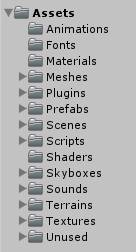
\includegraphics[]{img/Developpement_AssetHierarchy.PNG}}
			\captionof{figure}{Contenu du répertoire "Assets".}
			\label{structProjet}
		\end{minipage}\medskip
		
		Voici une description de leurs contenus:
		\begin{itemize}
			\item \textbf{Animations --} Ce répertoire contient tous les objets \textit{Animator} et \textit{Animations} créés dans ce projet. Les animateurs sont nommés "XAnimator" et les animation "XY" où X est le type d'objet à animer (\textit{e.g.}, "Gate") et Y est l'action réalisée (\textit{e.g.}, "Open"). Si le contrôleur ne contient qu'une animation, celle-ci se nomme "XAnimation". Toutes les animations ne sont pas présentes dans ce dossier. Celles provenant de sources trouvées sur internet (\textit{e.g.}, les animations de marche) se trouvent dans des sous-dossiers du dossier "\textit{Plugins}" décrit plus bas dans cette liste;
			\item \textbf{ Fonts --} Ce répertoire contient les polices de caractères utilisées dans ce projet;
			\item \textbf{ Materials --} Ce répertoire contient tous les objets \textit{Material} créés ou modifiés dans ce projet. Tous les matériaux du SG ne sont pas présents dans ce répertoire. Les matériaux créés automatiquement durant l'importation d'objets 3D sont présents dans le répertoire de destination de cette importation. Celui-ci étant un sous-répertoire de "Meshes" décrit plus bas dans cette liste; 
			\item \textbf{Meshes --} C'est dans ce répertoire que tous les modèles 3D (tel que \textit{.obj} ou \textit{.fbx}) trouvés sur internet sont importés. Chaque modèle est importé dans son propre sous-répertoire et certains sont regroupés en famille dans d'autres. L'importation crée de nombreuses ressources textures ou \textit{Material}. Celles-ci ne sont pas déplacées dans les répertoire "Textures" ou "Materials" mais laissées dans le sous-répertoire de l'importation.
			\begin{itemize}
				\item \textbf{Avatar --} Ce répertoire contient quatre sous-répertoires. Deux pour la tête et le costume d'un avatar féminin et deux pour ceux masculin. Dans le SG, seul le modèle féminin est utilisé actuellement. Si l'indication du sexe du patient peut être communiquée au SG, il est possible de lui choisir un avatar adapté;
				\item \textbf{Decorations --} Ce répertoire contient les différents modèles 3D utilisés en décoration dans les mondes (\textit{e.g.}, planètes, cascade, etc.). Ce sont des objets placés dans les mondes manuellement et ne subissant pas d'appauvrissement géométrique ou quantitatif;
				\item \textbf{Interior --} Ce répertoire contient les différents modèles 3D utilisés pour créer l'intérieur du vaisseau spatial (zone familière);
				\item \textbf{Landscape Elements --} Ce répertoire contient les différents modèles 3D utilisés pour créer les "\textit{Landscape elements}". Ce sont les objets placés massivement par script dans la scène dont la géométrie et la quantité peuvent être appauvries. Les modèles 3D de ce répertoire corresponde à leur modélisation totale ("\textit{FullGeometry}, voir section \ref{sDevAppauvrissement});			
				\item \textbf{Objectives --} Ce répertoire contient les différents modèles 3D utilisés pour les objectifs placés dans la scène;			
				\item \textbf{Spaceship --} Ce répertoire contient les différents modèles 3D du vaisseau spatial.	
			\end{itemize}
			\item \textbf{Plugin --} Ce répertoire contient les différents modules d'extension, les packs de ressources trouvés sur l'\textit{Assets store} \cite{UnityAssetStore_website} de \textit{Unity} ou encore les librairies (\textit{.dll}) utilisées par le SG.
			\begin{itemize}
				\item \textbf{Oculus --} Module d'extension pour l'utilisation de l'\textit{Oculus Rift} \cite{OculusDk2_website}. Depuis la version 5.1 \cite{UnityOculusIntegration}, \textit{Unity} ne nécessite plus de \textit{plugin} pour fonctionner avec ce HMD. Cependant, le résultat obtenu était perceptiblement plus saccadé que lors de l'utilisation du \textit{plugin}, c'est pourquoi il est encore utilisé dans ce travail. Ce phénomène a été constaté visuellement et aucune mesure n'a été faite. Sa source ou sa possible reproduction dans d'autres situations est inconnue. Ce n'est donc qu'une expérience vécue et non un fait avéré; %TOO: Jugement de valeur, à faire valider par STG
				\item \textbf{Raw Mocap Data --} Ce paquet est mis à disposition gratuitement par \textit{Unity}. Il contient différentes animations de marche, course, saut, etc. pour animer un avatar humanoïde. C'est de ce paquet que vient l'animation de marche du guide;
				\item \textbf{SG\_LHS --} Ce répertoire contient les deux librairies utiles à la communication avec le LHS. Celles-ci sont détaillés dans la sous-section précédente;
				\item \textbf{Standard Assets --} Ce paquet est mis à disposition gratuitement par \textit{Unity}. Il contient un certain nombre d'effets implémentés dans des scripts et des \textit{shaders}. Il est utilisé pour l'effet de flou de mouvement lors d'une téléportation.
			\end{itemize}
			\item \textbf{Prefabs, Scenes, Scripts --} Ces répertoires contiennent respectivement les \textit{Prefabs}, scènes et scripts. Chacun d'entre eux a une structure et une importance plus grande que les autres répertoires décrits dans cette sous-section. C'est pourquoi, une sous-section entière est dédiée à chacun d'eux, plus bas dans ce document;
			\item \textbf{Shaders --} Ce répertoire contient les différents \textit{shaders} écrits pour le SG;
			\item \textbf{Skyboxes --} Ce répertoire contient les différentes \textit{skyboxes} utilisées dans les différents mondes. Elles ont été trouvées sur internet;
			\item \textbf{Sounds --} Ce répertoire contient un sous-répertoire pour chaque type de son (détaillés dans la section \ref{sDevAppauvrissement});
			\item \textbf{Terrains --} Ce répertoire contient un sous-répertoire pour chaque niveau. Ceux-ci contiennent:
			\begin{itemize}
				\item Une image représentant le monde (utilisée dans le choix des niveaux);
				\item Trois fichiers de terrains, étant les trois niveaux d'appauvrissement de sa géométrie (voir section \ref{sDevAppauvrissement});
				\item Une "\textit{LandscapeElementsMap}", étant une image permettant la génération des "\textit{Landscape elements}" (voir \ref{sDevDeroulementPartie});
				\item Un fichier XML décrivant le chemin. Celui-ci décrit le chemin qui est imposé à l'utilisateur pour ce niveau. Plus de détails sur sa création et son utilisation dans la section \ref{sDevDeroulementPartie}.
			\end{itemize}
			
			\item \textbf{Textures --} Ce répertoire contient les textures créées ou manuellement assignées aux objets du SG. Les textures issues de l'importation de modèles 3D ou générée par scripts se trouvent, quant à elles, dans les répertoires de destination de ces importations ou générations. Les textures utilisées pour l'interface graphique ou le HUD sont, elles, importées en tant que \textit{sprites} et présentes dans le sous-répertoire "UI". Ce sous-répertoire contient également les fichiers de dessin de ces différents boutons ou icônes. Ces fichier ".svg" sont réalisés avec le logiciel \textit{Inkscape}, un logiciel libre de dessin vectoriel \cite{Inkscape_website}. Le sous-répertoire "Ground" contient toutes les textures utilisées sur les terrains. Le sous-répertoire "RenderTextures" contient toutes les \textit{RenderTextures} utilisées dans ce travail. Ces dernières permettent d'afficher en tant que texture ce que voit une caméra. D'autres textures sont directement contenues dans ce répertoire. C'est le cas de celles placées directement dans les scènes en décoration. La texture "\textit{Space Traveling in the speed of light - Royalty Free Footage}" a la particularité d'être une texture animée (vidéo). Elle nécessite d'avoir \textit{Quicktime} \cite{QuickTime_website} installé pour être importée correctement \cite{UnityMovieTexture}.
			%TODO: Faire une section Prérequis ?
		\end{itemize}	
		
	\subsection*{Structure des \textit{Prefabs}}
		Les \textit{Prefabs} sont des \textit{GameObject} (éléments composant les scènes) dont la configuration est enregistrée. Ceux-ci peuvent être utilisés dans plusieurs scènes et y être instanciés dynamiquement. Une modification sur un objet préfabriqué, l'applique à chacune de ses utilisations. Il est recommandé, même si un objet est utilisé dans une seule scène \cite{Unity50Tips} d'en créer un objet préfabriqué. Cela minimise les changements sur la scène et facilite la résolution de conflits, si on utilise un serveur de versionnement. Dans ce travail, de nombreux objets préfabriqués ont été créés. Ceux-ci se trouvent dans le répertoire "Prefabs" (figure \ref{structPrefabs}).\medskip
		
		\begin{minipage}{\linewidth}
			\makebox[\linewidth]{
				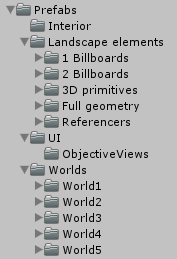
\includegraphics[]{img/Developpement_StructurePrefabs.PNG}}
			\captionof{figure}{Contenu du répertoire "Prefabs".}
			\label{structPrefabs}
		\end{minipage}\medskip
		
		Ce répertoire contient quelques objets préfabriqués ainsi que des sous-répertoires. Premièrement, voici une liste des objets préfabriqués qu'il contient:
		\begin{itemize}
			\item \textbf{ComputationalAvatar --} Cet objet est chargé si on utilise en entrée le clavier (quand le SG n'arrive pas à se connecter au LHS). Il contient un avatar invisible sur lequel est effectué une animation de marche lorsque l'on avance (flèche haut ou touche "w"). L'angle des articulations est ensuite relevé, par le script gérant les entrée/sorties, puis transmis à l'avatar principal pour l'animer en fonction;
			\item \textbf{Controllers --} Cet objet préfabriqué est contenu dans chaque niveau et contient tous les scripts contrôleurs utiles au déroulement d'une partie \cite{UnityMVC} (structure des scripts expliquée dans la section suivante);
			\item \textbf{EnterSceneAnimator --} Cet objet préfabriqué est contenu dans tous les mondes et l'animation d'atterrissage en début de niveau;
			\item \textbf{Guide --} Cet objet préfabriqué contient le guide et est présent dès la scène de sélection du niveau (structure des scènes expliquée dans une autre sous-section);
			\item \textbf{ImpoverishmentControllers --} Cet objet préfabriqué contient tous les scripts contrôleurs de l'appauvrissement. Il est présent dès la scène de sélection des niveaux;
			\item \textbf{Models --} Cet objet préfabriqué est présent dans la scène de sélection des niveaux. Il contient les différents modèles \cite{UnityMVC} nécessaires au fonctionnement du SG;
			\item \textbf{Objective --} Cet objet est à ajouter à chaque objet 3D représentant un objectif dans les scènes de jeu. Une fois placé et configuré (voir section \ref{sDevDeroulementPartie}), il les rend disponible au \textit{scan} et permet leur placement sur la gauche ou sur la droite du chemin.
			\item \textbf{ObjectiveMiniMapView --} Cet objet préfabriqué est instancié dynamiquement dans les niveaux. Il représente la zone où un objectif est présent sur la carte;
			\item \textbf{PlayerFemale, PlayerMale --} Ces objets préfabriqués sont, respectivement, l'avatar homme et femme. Le SG ne pouvant pas récupérer l'information du sexe du patient, seul l'avatar femme est utilisé pour le moment. Il est présent dès la scène de sélection des niveaux;
			\item \textbf{SpaceshipWithInterior --} Cet objet préfabriqué contient le vaisseau et ses pièces intérieures. Il est présent dès la scène de sélection des niveaux;
			\item \textbf{TeleportationRings --} Cet objet est instancié dynamiquement, si le temps dans un niveau est écoulé. Il contient les anneaux de téléportation se plaçant autour du joueur.
		\end{itemize}
		
		Deuxièmement, voici une description des sous-répertoires:
		\begin{itemize}
			\item \textbf{Interior --} Ce sous-répertoire contient les objets préfabriqués utilisés pour meubler l'intérieur du vaisseau spatial. Ce sont les objets qui sont considérés comme des éléments familiers;
			\item \textbf{Landscape elements --} Ce sous-répertoire contient un répertoire pour chaque type de géométrie des \textit{landscape elments}. Ceux-ci contiennent chacun un objet préfabriqué ou un autre répertoire pour chaque type ou famille de \textit{landscape elments}. Les \textit{landscape elments} étant les objets placés par script sur le terrain dont la géométrie et la quantité peuvent être appauvries (voir section \ref{sDevAppauvrissement}). Il contient également un sous-répertoire "Referencer". Celui-ci contient les \textit{landscape elments} référençant chacune de leur géométrie;
			\item \textbf{UI --} Ce sous-répertoire contient les objets préfabriqués utilisés dans l'interface de sélection des niveaux. Il contient un répertoire "ObjectiveViews" contenant les aperçus de tous les objectifs;
			\item \textbf{Worlds --} Ce sous-répertoire en contient un pour chaque niveau. Chacun contient les objets préfabriqués propres à chaque niveau. Voici une description de leur contenu:
			\begin{itemize}
				\item \textbf{Decorations --} Répertoire non obligatoire. Contient toutes les décorations utilisées dans le monde. Une décoration étant un objet n'ayant aucune interaction ni appauvrissement géométrique et quantitatif;
				\item \textbf{Landscape elements Families --} Répertoire obligatoire. Contient les différentes familles de \textit{landscape elments} utilisées dans le niveau;
				\item \textbf{Objectives --} Répertoire obligatoire. Contient tous les objectifs configurés du niveau;
				\item \textbf{GroundTerrain --} Objet préfabriqué obligatoire. Référence les bruits de pas pour chaque type de sol (voir section \ref{sDevAppauvrissement});
				\item \textbf{LevelX --} Objet préfabriqué obligatoire. Référence les différents éléments de visualisation du niveau (pour la sélection), ainsi que les éléments nécessaires au chargement de celui-ci.
			\end{itemize}
			
			Ce répertoire contient également un objet préfabriqué nommé "\textit{TerrainElements}". Il doit être placé dans toutes nouvelles scènes en tant qu'enfant de l'objet "Terrain". Il contient les principaux éléments d'un Terrain: La caméra affichant la mini-map, les lumières et la source audio de la musique de fond.
		\end{itemize}
	
	\subsection*{Structure des scripts}
		La structure des scripts suit le patron d'architecture modèle-vue-contrôleur (MVC) \cite{UnityMVC}, présenté dans la figure \ref{structScripts}. De façon générale, elle veille à minimiser l'interdépendance des script, afin de faciliter l'ajout ou la suppression d'une fonction.\medskip
		
		\begin{minipage}{\linewidth}
			\makebox[\linewidth]{
				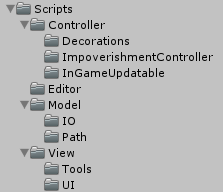
\includegraphics[]{img/Developpement_StructureScripts.PNG}}
			\captionof{figure}{Contenu du répertoire "Prefabs".}
			\label{structScripts}
		\end{minipage}\medskip
		
		Le dossier contient deux scripts: "\textit{SGMonoBehaviour}" et "\textit{InGameUpdatableSGMonoBehaviour}", dont la structure est schématisée dans un diagramme UML, en annexe. Le premier dérive de la classe "\textit{MonoBehaviour}". Cette classe \textit{Unity} est celle qu'un script doit hériter s'il veut être accroché dans la scène à un \textit{GameObject}. La classe "\textit{SGMonoBehaviour}" implémente des méthodes supplémentaires permettant de récupérer les objets de la scène implémentant une interface. La classe \textit{GameObject} propose de telles méthodes mais qui ne fonctionnent qu'avec les classes héritant de \textit{UnityEngine.Object}. Ces fonctions ont été trouvées sur un article proposant des bonnes pratiques pour le développement \textit{Unity} \cite{Unity50Tips}. Tous les scripts de ce travail devant être accroché à un \textit{GameObject} héritent donc de \textit{SGMonoBehaviour} (ou d'une classe enfant).
		\\
		
		La deuxième de ces classes est dérivée par tous les scripts devant être mise à jour à chaque moment d'un niveau du SG. Elle permet de définir un comportement pour les états de pause et de fin de jeu, ainsi que d'implémenter une logique d'activation ou de désactivation. Elle offre également une référence directe à la classe \textit{GameController}. Pour cela, il faut utiliser les méthodes "\textit{\_Start()}" et "\textit{\_Update}" au lieu de "\textit{Start()}" et "\textit{Update}".
		\\
		
		Quatre sous-répertoires sont ensuite présents: "\textit{Model}", "\textit{View}", "\textit{Controller}" et "\textit{Editor}". Les trois premiers contiennent les classes modèles, vues et contrôleur d'après le modèle MVC \cite{UnityMVC}. Le dernier contient les scripts éditeurs implémentés. Ces scripts permettent d'utiliser le package "\textit{UnityEditor}". Ils ne peuvent être intégrer dans les exécutables générés, c'est pourquoi ils ne doivent pas être utilisés dans les scènes de jeu et être contenu dans un dossier nommé  "\textit{Editor}". Certains de ces scripts ajoutent des fonctionnalités à l'environnement (\textit{e.g.}, "\textit{ApplyGameObjectMap}", "\textit{ExportSplatmap}" "\textit{InvertNormals}", "\textit{MergeMeshes}" ou "\textit{UnityEditor}"). D'autres modifient l'inspecteur de certains scripts (\textit{e.g.},  "\textit{ImpoverishmentModelEdiotr}" ou "\textit{HoverButtonEditor}"). D'autres encore, permettent d'accéder à la structure du projet pour charger ou créer des \textit{assets} (\textit{e.g.}, "\textit{BillboardGenerator}" ou "\textit{ObjectiveViewGenerator}").
		\\
		
		Le répertoire "\textit{Model}" contient deux sous-répertoires ainsi que divers scripts. Ces derniers contiennent peu de logique métiers et font souvent office d'ensemble de variables ou référencent des \textit{assets}. Mis à part le script "\textit{UnlockableObjectiveScannable}" et ses classes parentes, aucun ne contient de logique devant être exécutée à chaque instant. Ils n'héritent donc pas de \textit{InGameUpdatableSGMonoBehaviour} mais de \textit{SGMonoBehaviour}. %TODO: Corriger cette exception montrant un non-respect évident du modèle MVC...
		Aucun des scripts présents dans les deux répertoires n'héritent de \textit{InGameUpdatableSGMonoBehaviour}. Certains héritent de \textit{SGMonoBehaviour} et d'autres d'aucune classe et sont donc instanciés depuis d'autres scripts et non liés directement à des \textit{GameObjects}. Le premier de ces répertories, "\textit{IO}", contient tous les scripts utiles pour la gestion des entrées et sorties (voir section \ref{sDevDeroulementPartie}). Le second, "\textit{Path}", contient tous les scripts utiles pour générer le chemin que le joueur doit suivre (voir section \ref{sDevDeroulementPartie}).
		\\
		
		Le répertoire "\textit{View}" contient deux sous-répertoires et des scripts. Ces derniers référencent des composants et contiennent de la logique liée uniquement au retour d'informations à l'utilisateur (visuel et auditif). Le premier sous-répertoire, "\textit{Tools}" contient différents outils. Ces derniers, permettant principalement d'afficher des informations supplémentaires sur certains objets utiles pour le développement. Ces informations sont affichées uniquement dans "\textit{Gizmos}" (outil de visualisation de la scène de \textit{Unity}). Un exemple de ces informations est le dessin de tracé du chemin, comme le montre la figure \ref{PathInGizmos}. Le second sous-répertoire, "\textit{UI}", contient toutes les classes utilisant l'espace de nom "\textit{UnityEngine.UI}" et, donc, les composants d'interfaces graphiques. Ceux-ci sont présents dans le SG à l'écran de fin, pour le HUD (informations à l'écran durant la partie), ainsi que pour le choix des niveaux.
		
		Le répertoire "\textit{Controller}" contient trois sous-répertoires et trois scripts. Les scripts "\textit{GateController}" et "\textit{SpaceshipController}" sont les deux seuls à être des contrôleurs présents depuis la scène de sélection des niveaux. Ils n'héritent donc pas de "\textit{InGameUpdatableSGMonoBehaviour}". Le troisième script, "\textit{GameController}" est la dernière exception et n'en hérite également pas. Ce script est disponible directement à tous les autres contrôleurs qui sont présents dans le dossier "\textit{InGameUpdatable}". Le dossier "\textit{ImpoverishmentController}" contient tous les scripts contrôlant l'appauvrissement. Ils sont présents dès la scène de sélection des niveaux et héritent tous de la classe "\textit{ImpoverishmentController}" (voir section \ref{sDevAppauvrissement}). Le dernier dossier, "\textit{Decorations}" contient différents scripts utiles aux décorations. Ces scripts sont donc présents dans les niveaux. Ils gèrent les animations ou les déplacements de ces décorations.
		
	\subsection*{Structure des scènes}
		Dans cette sous-section sont expliquées les structures des différentes scènes. Il est également expliqué comment les différents composants (contrôleur d'entrée/sorties et \textit{Oculus Rift}) sont interfacés. De façon générale, nombre de \textit{GameObjects} ne servent qu'à instancier les scripts qui leurs sont attachés et n'ont pas d'autres contenus. Ceux-ci sont donc placés en position et orientation par défaut (0,0,0). Les coordonnées du monde peuvent correspondre à une échelle métrique doublée. Le joueur a une taille de 3.6, ce qui correspond à 1 mètre et 80 centimètres. %TODO: Changer ça pour que ça corresponde.
		Aucune lumière ambiante n'est présente dans les scènes de jeu.
		
		Le dossier scène contient un répertoire, la scène de sélection des niveaux et une scène par niveau.
		\\
		
		Le répertoire, "\textit{Tools}" contient différentes scènes de démonstration ou utilitaires. Les scènes "\textit{BillboardGenerator}" et "\textit{ObjectiveViewGenerator}" permettent de générer respectivement des objets préfabriqués "\textit{BillboardCloud}" (voir section \ref{sDevAppauvrissement}) et les images d'aperçu des objectifs (pour le choix des niveaux). Ces scènes utilisent les scripts "\textit{BillboardGenerator}" et "\textit{ObjectiveViewGenerator}" qui utilisent des fonctionnalités du paquet "\textit{UnityEditor}". Ces scripts sont dans le dossier "\textit{Scripts/Editor}" d'où ils ne peuvent être accrochés à un \textit{GameObject}. Pour se servir de ces scènes, il faut d'abord sortir le script du dossier et le référencer dans \textit{GameObject} du même nom que la scène. Ensuite, il faut placer l'objet dont on souhaite générer un "\textit{BillboardCloud}" ou son aperçu au centre de la boite, "\textit{Box}", (indiquant la proportion de l'image qui sera générée). Pour redimensionner cette boite, il faut modifier le paramètre "\textit{size}" du script. Une fois la boîte redimensionnée correctement et l'objet placé au centre, il suffit de presser "\textit{Play}". Cela va créer un \textit{BillboardCloud}, un objet préfabriqué "BillboardCloud.prefab", dans le dossier "Assets/Prefabs/Landscape elements/Gen/X Billboards" où X est le paramètre "Nb Planes" du script. Pour la création de l'image de l'objectif, cela crée une image "ObjectiveView.png" dans le répertoire "Assets/Textures/UI/Objectives/Gen/".
		\\
		
		%Sélection des niveaux
		La scène de sélection du niveau est la première scène chargée par le SG. Son éclairage provient des objets "\textit{LightBulb}" placé dans chaque pièce. Leur source de lumière étant à chaque fois de type "point". Elle contient tous les \textit{GameObjects} communs à chaque scène. Ils sont conservés une fois la scène du niveau choisit car le chargement de la nouvelle scène se fait de façon additive. La figure \ref{HierarchyLevelSelection} montre le contenu de cette scène.\medskip		
		
		\begin{minipage}{\linewidth}
			\makebox[\linewidth]{
				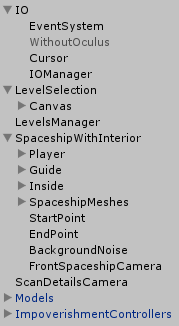
\includegraphics[]{img/Developpement_HierarchieLevelSelection.PNG}}
			\captionof{figure}{Contenu de la scène de sélection du niveau.}
			\label{HierarchyLevelSelection}
		\end{minipage}\medskip
		
		"\textit{IO}" contient tous les éléments utiles pour l'interaction de l'utilisateur: "\textit{IOManager} s'occupe d'instancier le bon "\textit{IOController}" en fonction de la disponibilité ou non du LHS; "\textit{Cursor}" est le curseur placé au centre de l'écran pour la sélection des niveaux; "\textit{WithoutOculus}" permet, quand il est activé, de contrôler l'orientation de la caméra avec la souris (ce qui permet de tester le SG sans \textit{Oculus Rift}).
		
		"\textit{LevelManager}" référence les niveaux à afficher et permet d'en charger un. "\textit{Models}" contient le modèle d'appauvrissement, celui du profil du patient, celui caractérisant le niveau d'aide demandé et celui permettant la gestion de la persistance. "\textit{ImpoverishmentControllers}" contient tous les scripts contrôlant l'appauvrissement de la scène.
		"\textit{LevelSelection}" contient le canevas de l'interface graphique du choix des menus. Ces menus ne nécessitent pas de souris et les boutons sont activés au survol. Un laps de temps avant l'activation est possible (utilisé pour la sélection d'un niveau et le clic sur le bouton de lancement du niveau). Le déplacement d'un curseur d'après le regard est implémenté d'après un article \cite{UnityUISystemInVR} dans la catégorie "développeur" du site d'\textit{Oculus Rift}. Pour la sélection au survol, une nouvelle classe, "\textit{HoverButton}", héritant de \textit{UnityEngine.UI.Button} a été réalisée. Le reste de l'intégration de l'\textit{Oculus Rift}, est réalisée à l'aide du \textit{plugin} fournit par Oculus.
		
		"\textit{SpaceshipWithInterior}" contient, entre autres, tous les éléments ayant une modélisation de la scène (\textit{i.e.}, le vaisseau spatial, les pièces intérieures et leur contenu, le joueur et le guide). Plus de détails sur le joueur, le guide ou encore l'intérieur du vaisseau (zone familière) sont présentés dans la section \ref{sDevAppauvrissement}. L'objet préfabriqué contient également deux points marquant le point de départ du joueur ainsi que celui de sortie du vaisseau spatial. Ces points sont des \textit{GameObjects} vides avec un script attaché permettant de dessiner dans l'éditeur de scène une sphère en fil de fer pour indiquer leur position. Un son est également contenu. Celui-ci correspond à un bourdonnement de moteur. Il correspond à un son d'ambiance, c'est pourquoi il nécessite d'être dans un \textit{GameObject} avec le \textit{tag} "\textit{BackgroundSound}". Pour finir, il contient également une caméra placée à l'avant du vaisseau. Celle-ci sert durant la transition entre les scènes, visible dans la figure \ref{SceneTransition}.
		\\
	
		%TODO: Déplacé ça dans le déroulement d'une partie plutôt
		La transition entre les scènes se lance une fois un niveau choisit sur l'écran devant le joueur et le bouton vert pressé. Le chargement asynchrone de la nouvelle scène (\textit{i.e.}, tous les \textit{GameObjects} de la scène actuelle sont conservés) est lancé et une animation est lancée sur l'écran. Cette animation est une vidéo lancée dans une texture sur le même écran dans la scène. Après la vidéo, la texture de l'écran affiche le contenu de la caméra devant le vaisseau qui effectue une trajectoire l'amenant de la coordonnée (0,1000,0) au début du parcours à l'aide d'une interpolation sphérique \cite{UnityVector3Slerp}. Une fois arrivé au début du parcours, le HUD est chargé, l'écran remonte, les portes s'ouvrent et les mouvements du joueur sont débloqués. Ces différentes étapes sont visibles dans la figure \ref{SceneTransition}.\medskip%TODO: Voir si on peut envoyer le start ici au LHS
		
		\begin{minipage}{\linewidth}
			\makebox[\linewidth]{
				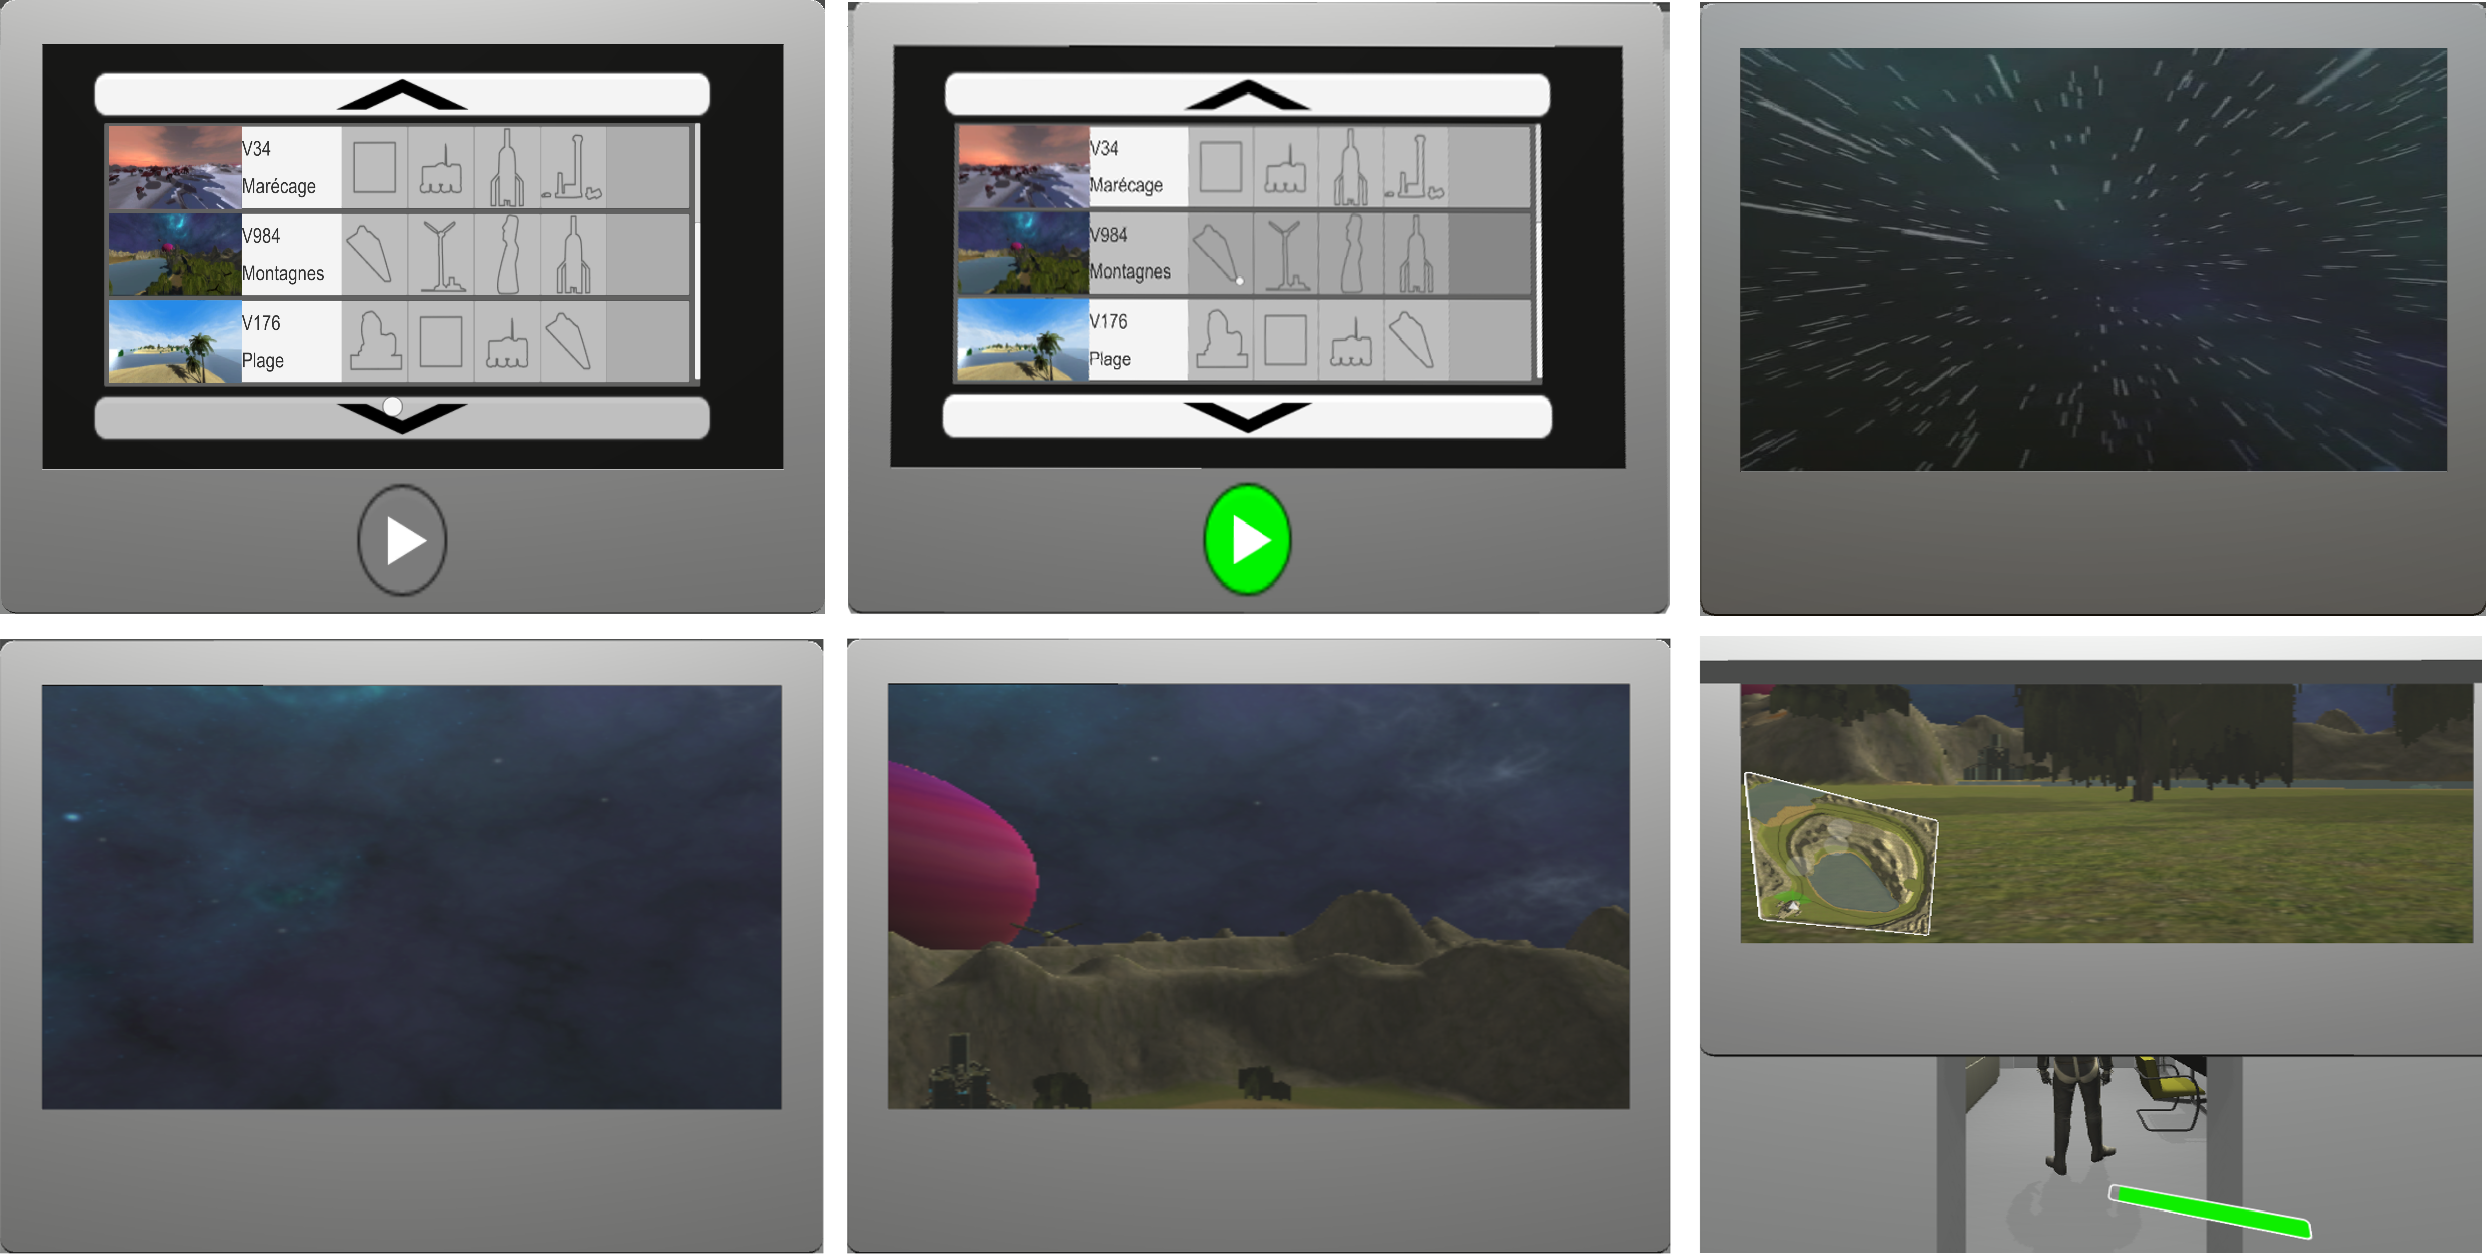
\includegraphics[width=\textwidth]{img/Developpement_LevelTransition_2_Reduced.png}}
			\captionof{figure}{Transition entre les scènes, dans le sens de lecture.}
			\label{SceneTransition}
		\end{minipage}\medskip
		\\	
	
		%Niveau de jeu
		Les scènes des niveaux sont nommées \textit{WorldX} où X représente le numéro du niveau. Ces numéros doivent être uniques et définissent l'ordre d'affichage sur l'écran de choix des niveaux. Elles contiennent toutes une structure similaire visible sur la figure \ref{HierarchyWorld}.\medskip
		
		\begin{minipage}{\linewidth}
			\makebox[\linewidth]{
				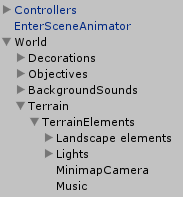
\includegraphics[height=\imgHeightSmall{}]{img/Developpement_HierarchieWorld.png}}
			\captionof{figure}{Contenu de la scène d'un niveau.}
			\label{HierarchyWorld}
		\end{minipage}\medskip
		
		Le \textit{GameObject} "\textit{Controllers}" contient les différents contrôleurs utiles au bon déroulement d'une partie. "\textit{EnterSceneAnimator}" gère l'animation d'atterrissage. Ces deux objets ne diffèrent pas d'un niveau à l'autre. Ils ne sont que des instances des objets préfabriqués du même nom. Ils ne servent qu'à l'instanciation des scripts qui leurs sont associés.
	
		Le dernier \textit{GameObject} se trouvant à la racine, "\textit{World}", contient tous les éléments composant le niveau. C'est en analysant récursivement ses enfants que les scripts contrôleurs d'appauvrissement récupèrent les références des objets à appauvrir. Il est donc important qu'aucun ne soit en dehors de cet objet. Ce dernier peut contenir jusqu'à quatre enfants: "\textit{Decorations}", "\textit{Objectives}", "\textit{BackgroundSounds}" et "\textit{Terrain}". "\textit{Decorations}" et "\textit{BackgroundSounds}" sont facultatifs et contiennent, respectivement, les éventuels éléments de décors et sons d'ambiance.  "\textit{Objectives}" contient tous les objectifs à trouver du niveau (contraintes des objectifs expliquées dans la section \ref{sDevDeroulementPartie}). "\textit{Terrain}", est l'objet \textit{Unity} terrain de la scène. Il possède également le script "\textit{ImpoverishableTerrain}" permettant de rendre son appauvrissement et ce celui de ses enfants possibles. Tout son contenu se trouve dans "\textit{TerrainElements}":%TODO: Mettre le contenu directement dans Terrain...
		\begin{itemize}
			\item \textbf{Landscape elements --} Cet objet contient trois enfants nommé "1", "2" et "3". Chacun contenant l'ensemble des "\textit{Landscape elements}" d'une famille. Ce \textit{GameObject} et son contenu sont générés à l'aide du script éditeur "\textit{ApplyGameObjectMap}". Plus de détails dans la section \ref{sDevAppauvrissement};%TODO Modifier ce GameObject pour respecter le CamelCase
			
			\item \textbf{Lights --} Contient toutes les lumières influençant l'éclairage du monde. Est composé de trois sources de lumière directionnelles s'inspirant de l'éclairage à trois points \cite{3PointsLightning} pour ne pas utiliser de lumière ambiante;
			
			\item \textbf{MinimapCamera --} Le résultat de cette caméra est rendu dans la texture utilisée pour la carte. Ne sont rendus sur cette caméra que les éléments présents sur la couche (\textit{layer}) "\textit{Terrain}";%TODO: Mettre les LandscapeElements et p-e même les objecifs sur cette couche, qu'on les voient sur la minimap
			
			\item \textbf{Music --} La source audio de la musique de fond. Ayant le tag "\textit{Music}" pour l'appauvrissement (voir section \ref{sDevAppauvrissement}). Elle peut donc être changée pour chaque niveau.
		\end{itemize}

\section{Appauvrissement de la scène}
	\label{sDevAppauvrissement}
	Dans cette section est détaillée l'implémentation des différents aspects de l'appauvrissement d'une scène. Ils se réfèrent à ceux définis dans la conception, section \ref{sConSelectionObjectifs}. Pour certains aspects de l'appauvrissement, des tests ont été réalisés en début de projet, avant même la conception. Ces tests sont détaillés dans chaque sous-section concernée. Ces derniers peuvent s'étendre en dehors des objectifs sélectionnés dans la section précédemment citée car ils ont été réalisés antérieurement.
	\\
	
	Chaque aspect de l'appauvrissement est géré par un script héritant de "ImpoverishmentController". Ceux-ci sont présent dès la scène de sélection des niveaux et se réfère au script "ImpoverishmentModel" pour connaître le niveau d'appauvrissement qu'ils doivent afficher. Certains de ces scripts nécessitent de recharger des éléments au chargement de la scène d'un niveau. C'est le script "GameController" présent dans cette dernière qui se charge de récupérer tous les contrôleurs d'appauvrissement et de leur demander de se mettre à jour. Pour cela, il leur donne une référence sur le \textit{GameObject} "World" contenant tous les éléments de la scène (voir section \ref{sDevStructure}).
	
	\subsection*{Appauvrissement géométrique des \textit{Landscape elements}}
		
		Parmi les éléments placés sur les terrains, seuls les \textit{landscape elements} offrent un appauvrissement géométrique. En d'autres termes, le vaisseau, les personnages, les objectifs et les décorations n'ont pas d'appauvrissement géométrique.
		Les \textit{landscape elements} sont les éléments placés en masse sur le terrain par un script (voir \ref{sDevDeroulementPartie}) servant à meubler l'environnement et ayant un appauvrissement géométrique et quantitatif. Dans cette sous-section, seul leur l'appauvrissement géométrique est détaillé.
		\\
	
		Pour cet aspect, plusieurs versions tests ont été réalisées avant même la conception. La première version (figure \ref{ObjectLibraryV1}) consiste à proposer des modélisations complètes d'objets pour les trois derniers niveaux d'appauvrissement. Ces objets ayant une nature de complexité croissante avec le niveau, par exemple: pour le niveau deux, cristal; pour le trois, arbre mort (sans feuillage); pour le quatre, arbre avec feuillage. Le premier niveau de complexité quant à lui consiste en de simples primitives géométriques. Plus on monte dans les niveaux, plus les objets sont riches en couleurs et possèdent un aspect vivant (feuillage, mousse). Cette proposition va avec l'hypothèse de proposer une progression de l'appauvrissement calquée sur celle du jeu. Cette idée est détaillée dans la description du \textit{GamePlay}, chapitre Conception, section \ref{sConGameConcept}. Or, comme expliqué dans cette section, cette idée ne peut être retenue car un patient doit pouvoir réaliser tout le jeu indépendamment de ses capacités cognitives. Cette proposition diminue également la richesse du jeu, de l'appauvrissement (\textit{e.g.}, les couleurs étant liées à la géométrie). Elle est incohérente car un objet va changer de nature en fonction de son appauvrissement géométrique (\textit{e.g.}, un arbre devient un cristal puis un cône). Pour les multiples raisons citées, elle n'a pas été pas retenue.\medskip	
	
		\begin{minipage}{\linewidth}
			\makebox[\linewidth]{
				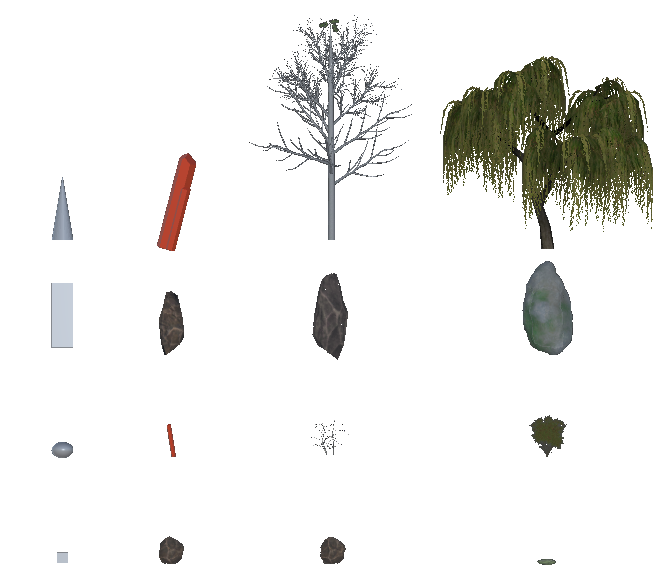
\includegraphics[height=\imgHeightMedium{}]{img/Tests_ObjectLibraryV1_2_Detoured.png}}
			\captionof{figure}{Librairie d'objets de décors, première proposition: nature de l'objet simplifiée. Horizontal: différentes géométries d'un objet. Vertical: différents objets pour la même géométrie.}
			\label{ObjectLibraryV1}%TODO: Refaire mais avec un fond blanc
		\end{minipage}\medskip
		\\	
		
		La version suivante est celle actuellement implémentée dans le SG. Elle respecte la contrainte de pouvoir reconnaître la nature d'un objet indépendamment du niveau d'appauvrissement (figure \ref{ObjectLibraryV2}). Ceux-ci ne peuvent alors plus se contenter de trouver des modèles d'objets de nature plus ou moins complexe mais doivent proposer des représentations différentes du même objet. L'idée étant de partir du modèle de l'objet trouvé sur internet (correspondant au plus haut niveau de détail) puis d'en proposer des géométries différentes.
		\\
		
		Plusieurs solutions ont été testées pour diminuer la complexité d'un objet. Premièrement, des recherches quant aux technologies de \textit{billboards cloud} ont été effectuées. Cette technique permet de modifier un modèle 3D composé de sommets et de polygones par un ensemble de \textit{billboards} \cite{Decoret_BillboardCloud, Lacewell_BillboardCloud, Behrendt_BillboardCloud, Garcia_BillboardCloud, Decoret_BillboardCloudExtrem}. Elle possède comme avantage d'alléger la charge de travail de la carte graphique. Il est envisageable, qu'en diminuant le nombre de \textit{billboards} on puisse également diminuer la complexité perçue de l'objet.
		
		La deuxième solution est la simplification du modèle 3D en diminuant le nombre de sommets ou de triangles \cite{Schroeder_DecimationTrianglesMeshes}.
		Cependant, leur implémentation a été jugée trop conséquente pour pouvoir respecter le reste des objectifs sélectionnés (section \ref{sConSelectionObjectifs}). Une autre piste était alors l'utilisation de logiciels proposant cette fonctionnalité. Aucun logiciel ne correspondait à toutes les attentes, la plupart étant payants \cite{Atangeo_webiste, Cruncher_UnityPlugin_website}. Le logiciel libre "\textit{Blender}" \cite{Blender_website} propose la fonctionnalité "Decimate" permettant de réduire le nombre de polygones. Après plusieurs tests effectués, il s'avère que le plaquage des textures et le calcul des normales est à refaire. Cette solution est restée une piste intéressante mais nécessite la maîtrise du logiciel, initialement destiné à des \textit{designers}. Cette solution n'a donc pas été exclue pour la suite du projet de recherche, mais sort du cadre cependant de ce travail de Master.
		\\
		
		Finalement la solution choisie pour être implémentée dans ce travail est la suivante. Ces géométries ont été choisies pour être réalisées facilement, sans logiciels payant et sans les compétence d'un \textit{designer}. Le niveau le plus riche est appelé "\textit{FullGeometry}". Trois appauvrissements sont proposés: ensemble de \textit{billboards}; primitives 3D; \textit{billboard}. L'appauvrissement "prmitives 3D" est à construire à la main dans Unity. Le but étant de reproduire la forme de l'objet de façon simple à l'aide de primitives 3D telles que des parallélépipèdes rectangles, des cônes, et des ellipsoïdes. Les géométries "ensemble de \textit{billboards}" et "\textit{billboard}" sont, quant à elles, générées (détails de leur génération dans la sous-section suivante).	Le \textit{billboard} est un quadrilatère sur lesquels est appliqué une texture avec de la transparence. Pour éviter de voir qu'il ne possède aucune épaisseur, il s'oriente d'après la caméra. L'ensemble de \textit{billboard}, aussi appelé "\textit{billboard cloud}" est composé de deux \textit{billboards} ne s'orientant pas avec la caméra et se coupant l'un l'autre en leur centre horizontal de façon perpendiculaire (figure \ref{BillboardCloud}). Pour chacune des deux représentations se servant de \textit{billboard}, deux variantes sont proposées: en tenant compte des normales ou en les ignorant (prenant ainsi les normales des quadrilatères). La version sans normales se comporte, face à la lumière, comme une surface plate. La version avec normales permet de simuler un relief. Il permet d'éclairer certaines parties et d'en assombrir d'autres comme si elles étaient orientées différemment.\medskip
		
		\begin{minipage}{\linewidth}
			\makebox[\linewidth]{
				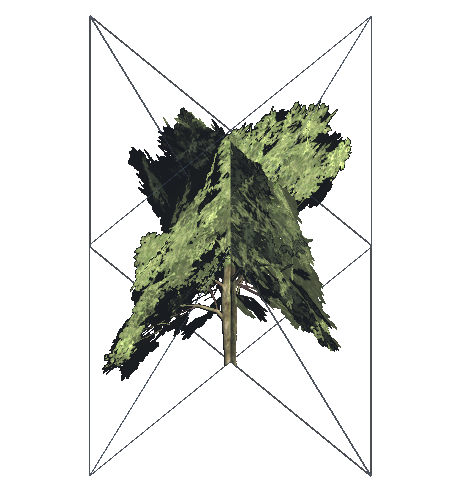
\includegraphics[height=\imgHeightMedium{}]{img/Tests_BillboardsCloudArengement2_Edited.PNG}}
			\captionof{figure}{Ensemble de \textit{billboards} représentant un arbre.}
			\label{BillboardCloud}
		\end{minipage}\medskip
	
		Dans la figure \ref{ObjectLibraryV2}, on voit les dix premiers objets (dix lignes) proposés pour cette technique d'appauvrissement et leurs six différentes géométries (six colonnes). Ces objets représentent, de haut en bas: un arbre; un arbre mort; un grand cristal; un rocher; une colonne de roche; un buisson; une petite plante; un petit cristal; un buisson mort. Même s'ils ne sont pas utilisés dans les niveaux actuels, ils sont tout de même présents dans les \textit{assets} du projet, dans "Prefabs/Landscape elements/". Triés dans des sous-répertoires par géométrie, dans l'ordre de la figure \ref{ObjectLibraryV2}: "Full geometry"; "2 Billboards"; "3D primitives"; "1 Billboards". Les versions avec et sans normales sont dans le même répertoire. Dans chacun de ces dossiers, ils sont ensuite triés par objet, de haut en bas: "Tree"; "Dead tree"; "Big crystal"; "Big rock"; "Stone column"; "Bush"; "Small plant"; "Small crystal"; "Dead bush". Ces noms sont directement attribués à l'objet préfabriqué pour les répertoires "Full geometry" et "3D primitives". Les répertoires de ceux utilisant des \textit{billboards}, contiennent un sous-répertoire du nom de l'objet. Pour le "2 Billboards", deux versions des objets préfabriqués sont présentes. Un pour la version avec normales et un pour celle sans. Ils se nomment respectivement "BillboardCloud\_n" et "BillboardCloud". Pour le "1 Billboards", les mêmes objets préfabriqués peuvent y être contenu, mais ils ne sont pas à utiliser car ils ne possèdent pas d'orientation d'après la caméra. Ils sont un résultat intermédiaire utile pour générer les objets préfabriqués souhaités. Ceux-ci sont présents dans le même dossier et se nomment "BillboardSinglePoint\_n" et "BillboardSinglePoint". La génération des géométries composées de \textit{billboards} est détaillée dans la sous-section suivante.
		
		\medskip
		\begin{minipage}{\linewidth}
			\makebox[\linewidth]{
				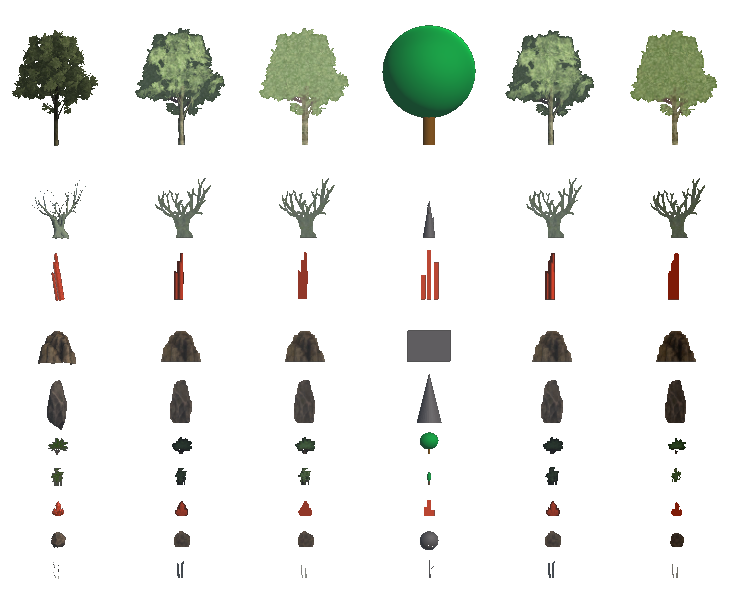
\includegraphics[width=\textwidth]{img/Tests_ObjectLibraryV2_2_Detoured.png}}
			\captionof{figure}{Librairie d'objets de décors, deuxième proposition: modélisation de l'objet modifé. Horizontal: différentes géométries d'un objet. Vertical: Différents objets pour la même géométrie.}
			\label{ObjectLibraryV2}
		\end{minipage}\medskip%TODO Refaire l'image sur fond blanc
		\\
		
		Il reste encore un type d'objet présent dans "Prefabs/Landscape elements/" non décrit: les référenceurs. Ils sont présents dans le sous-répertoire "Referencers". Il y en a un pour chaque type de \textit{landscape elements}. Ce sont des objets préfabriqués du nom de l'objet qu'ils représentent contenant le script "LandscapeElement". Celui-ci nécessite une référence pour chacune des différentes géométries de l'objet ainsi qu'une valeur "Min Radius Needed". Cette dernière représente la distance minimale entre le centre de ce \textit{landscape element} et un autre centre d'un autre \textit{landscape element}. Ce sont des objets qui sont placés dans la scène et qui, d'après les valeurs d'appauvrissement, chargent la géométrie adéquate. Le détail de ce placement est expliqué dans la section \ref{sDevDeroulementPartie}.
		\\
		
		De façon générale, chacune de ces géométries de chacun de ces \textit{landscape elements} doit avoir son pivot centré à la base (sol). Cela permet de simplement poser sur le sol les instances des objets préfabriqués et qu'elles soient alignées correctement. Certains types de \textit{landscape element} forment une famille (\textit{e.g.}, les champignons du monde 3). Ils possèdent différentes modélisations mais d'un objet de même nature. Chaque modélisation doit alors posséder son appauvrissement. Les objets préfabriqués de la même famille sont alors regroupés dans un répertoire parent.%TODO: Mieux expliquer ? avec une image ?
		
		Pour terminer cette sous-section, voici un aperçu du SG avec les différentes modélisations géométriques sont disponibles, figure \ref{DemoGeometryLandcapeElements}.\medskip		
		
		\begin{minipage}{\linewidth}
			\makebox[\linewidth]{
				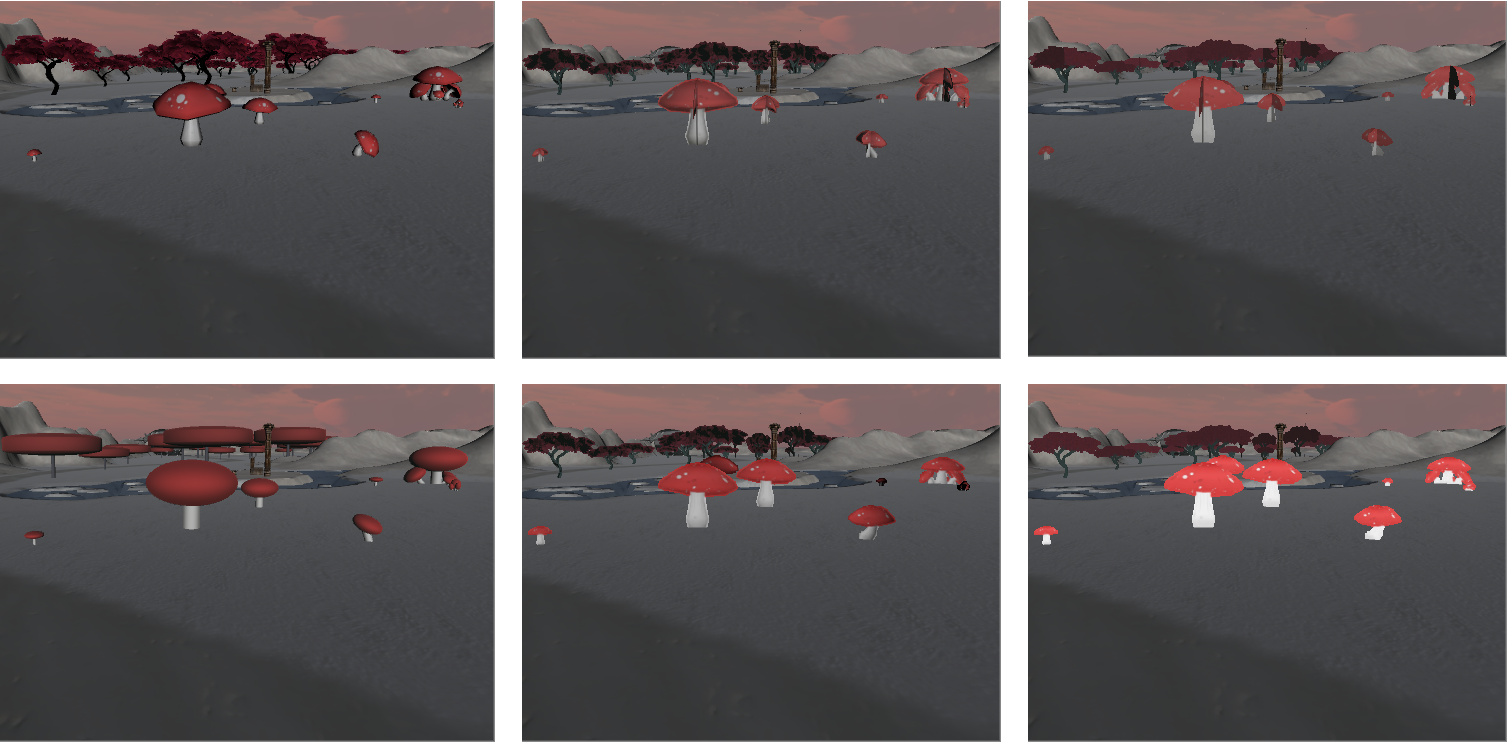
\includegraphics[height=\imgHeightMedium{}]{img/Developpement_DemoGeomLandscapeElem_Resized.png}}
			\captionof{figure}{Aperçu d'un niveau avec les différentes géométries pour les \textit{landscape elements}. Dans l'ordre de lecture: géométrie complète; 2 \textit{billboards} avec normales; 2 \textit{billboards} sans normales; primitives 3D; \textit{billboards} avec normales; \textit{billboards} sans normales.}
			\label{DemoGeometryLandcapeElements}
		\end{minipage}\medskip %TODO: À redimensionner (moins de place horizontale)		

	\subsection*{Génération des \textit{billboards} et ensembles de \textit{billboards}}
		La scène "BillboardGenerator" permet de générer les ensembles de \textit{billboards} (à un ou deux plan, mais ne suivant pas la caméra) grâce au script du même nom. Ce dernier utilisant des fonctionnalités du paquet \textit{UnityEditor}, il est placé dans le répertoire "Scripts/Editor" ignoré lors d'un \textit{build}. Cependant, il doit être référencé dans la scène et, par conséquent, sortit de ce répertoire pour effectuer les générations. Il est envisageable de modifier ce script pour qu'il ajoute une action dans l'éditeur plutôt qu'il doive être présent dans la scène, ce qui éviterait ce désagrément. Il faut ensuite placer le modèle souhaité dans la scène, en tant qu'enfant du \textit{GameObject} "BillboardGenerator". Il doit être centré dans la boîte transparente nommée "Box". La taille de celle-ci (indiquant la zone contenue dans l'image créée) peut être réglée avec le paramètre "Size" du script "BillboardGenerator", attaché au \textit{GameObject} du même nom. Il reste encore deux paramètres à régler, toujours sur le même script. Le premier, "Nb planes", décrit le nombre de plans utilisés. Il doit être paramétré à 2 pour générer la géométrie "2 Billboards". Le deuxième paramètre est "Normal map as Texture" et permet d'indiquer la texture servant de \textit{normal map} \cite{UnityNormalMap} de l'objet cible. S'il n'en a pas, ce paramètre peut être laissé vide.
		Une démonstration du placement et des paramètres de "BillboardGenerator" est visible dans la figure \ref{BillboardGeneratorSettings}.\medskip		
		
		\begin{minipage}{\linewidth}
			\makebox[\linewidth]{
				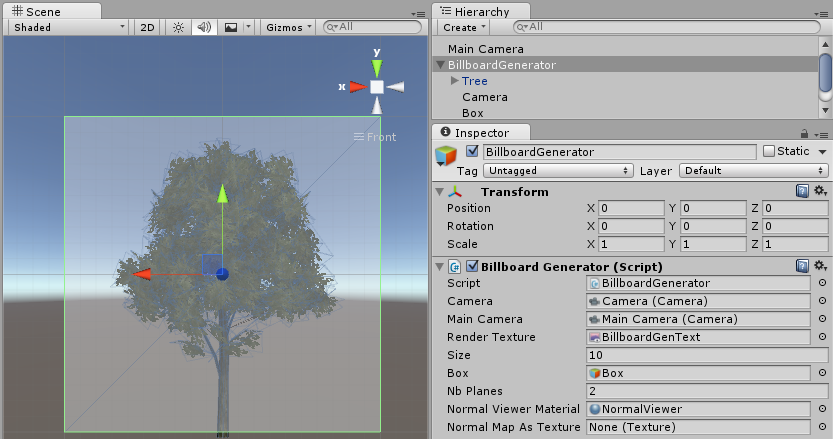
\includegraphics[height=\imgHeightMedium{}]{img/Developpement_BillboardGeneratorSettings.PNG}}
			\captionof{figure}{BillboardGenerator - Placement de l'objet et paramètres de BillboardGenerator.}
			\label{BillboardGeneratorSettings}
		\end{minipage}\medskip
		
		Une fois ces réglages effectués, il suffit de lancer la scène (presser "Play") et la génération se lance. Cette étape peut prendre un certain temps où \textit{Unity} peut ne pas répondre. Les objets préfabriqués "BillboardCloud" et "BillboardCloud\_n" sont créés et enregistrés dans le répertoire "Prefabs/Landscape elements/Gen/X Billboards" où "X" est le paramètre "Nb planes". Des instances de ces objets sont présentes dans la scène pour démonstration (voir figure  \ref{BillboardGeneratorGeneratedWithoutFoliage}). Pour les objets sans feuillage, il suffit de déplacer et renommer le répertoire "Gen" à l'endroit et avec le nom souhaité.\medskip		
		
		\begin{minipage}{\linewidth}
			\makebox[\linewidth]{
				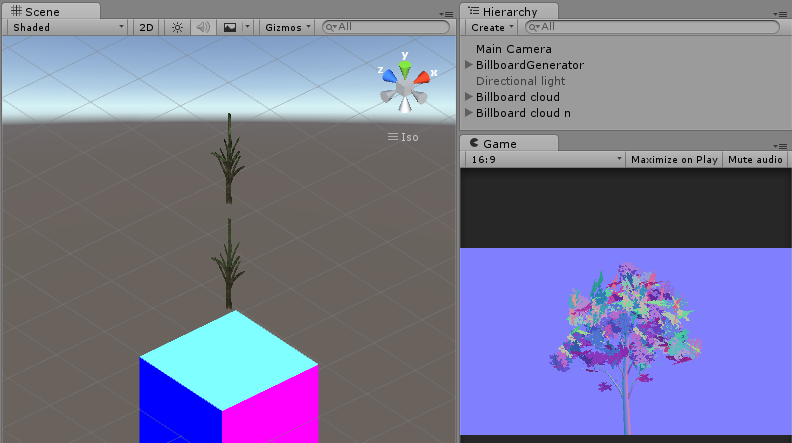
\includegraphics[height=\imgHeightMedium{}]{img/Developpement_BillboardGeneratorGeneratedWithoutFoliage.PNG}}
			\captionof{figure}{BillboardGenerator - Aperçu des objets générés.}
			\label{BillboardGeneratorGeneratedWithoutFoliage}
		\end{minipage}\medskip
		
		Pour les objets devant comporter un feuillage, celui-ci est, pour une raison inconnue, non visible. Il faut encore réaliser une étape contournant ce problème. Cette étape consiste à sélectionner les images "side0" et "side1" générée, cocher la case "Alpha from Grayscale" et appliquer les modifications (voir figure \ref{BillboardGeneratorGeneratedWithFoliage}).\medskip		
		
		\begin{minipage}{\linewidth}
			\makebox[\linewidth]{
				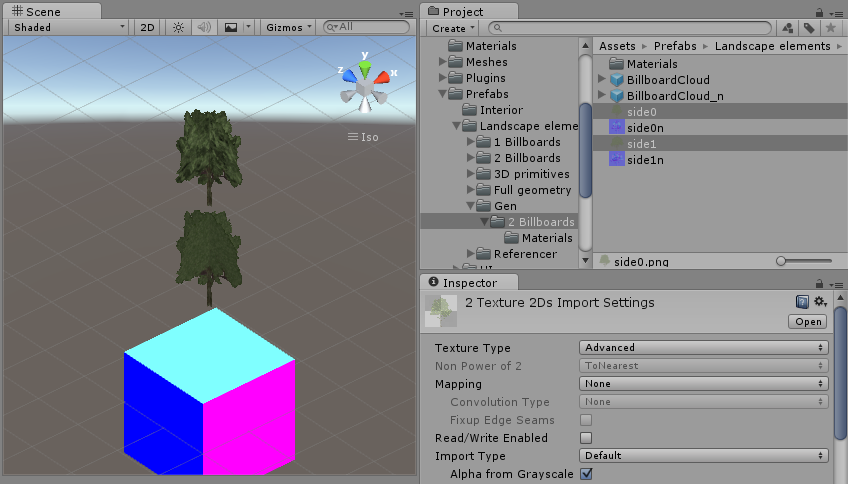
\includegraphics[height=\imgHeightMedium{}]{img/Developpement_BillboardGeneratorGeneratedWithFoliage.PNG}}
			\captionof{figure}{BillboardGenerator - Objet avec feuillage corrigé.}
			\label{BillboardGeneratorGeneratedWithFoliage}
		\end{minipage}\medskip
		
		Durant l'initialisation de la scène, la création de ces objets se réalise de la façon suivante. Premièrement, une caméra orthographique (n'ayant pas d'effet de perspective) est dimensionnée de façon à inclure tout le contenu de la boite. Elle est sur l'axe \textit{z} et regarde l'objet. Cette caméra rend son contenu dans une texture. Cette texture est copiée dans une image "side0.png". Si le paramètre "Nb planes" est plus grand que "1", elle va tourner autour de l'axe \textit{y}, toujours en regardant l'objet puis générer d'autres images. Ces rotations sont uniformément réparties entre 0 et 180°. Ces images sont ensuite appliquées comme texture à des \textit{material}. Ces derniers étant utilisés sur des primitives "\textit{Quad}". Chacune ayant la même orientation que la caméra avait pour générer l'image. Pour chaque plan, deux "\textit{Quad}" sont créés. Le deuxième ayant son \textit{scale} en y mis à "-1" afin de l'inverser horizontalement. Ceci crée l'objet "BillboardCloud", étant enregistré comme objet préfabriqué.
		\\
		
		Pour la version avec normales, une étape supplémentaire est réalisée. Celle-ci replace la caméra à son emplacement et orientation initiale. Elle applique ensuite à tous les enfants du \textit{GameObject} "BillboardGenerator", le \textit{material} "NormalViewer". Celui-ci utilise le shader "NormalViewing". Ce dernier est implémenté de façon à visualiser les normales et non les couleurs d'un objet (les couleurs des pixels rouge, vert et bleus prennent les valeurs x, y, z de la normale en ce point). Ces normales sont calculées par rapport à l'orientation des sommets ou d'après la \textit{normal map} donnée. Une fois que l'objet affiche les normales, la même étape de création d'image est réalisée. Cette fois, les images s'appellent "sideXn.png". De nouveaux \textit{materials} sont créés affichant "sideX.png" avec pour \textit{normal map} "sideXn.png".
		\\
		
		Pour créer les \textit{billboard} simples, il faut premièrement effectuer la même étape pour créer un ensemble de  \textit{billboards}, mais avec le paramètre "Nb planes" mis à "1". Ensuite, il faut sélectionner, dans les \textit{assets} un des objets préfabriqués créés. Puis, effectuer l'action "NWTools, Generate SinglePointBillboard" (figure \ref{GenerateSinglePointBillboard}).\medskip
		
		\begin{minipage}{\linewidth}
			\makebox[\linewidth]{
				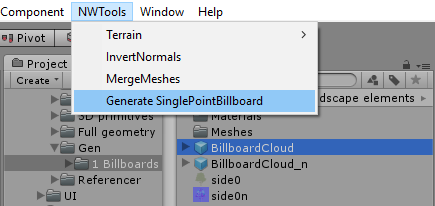
\includegraphics[height=\imgHeightSmall{}]{img/Developpement_GenerateSinglePointBillboard.png}}
			\captionof{figure}{Génération d'un \textit{billboard} suivant la caméra.}
			\label{GenerateSinglePointBillboard}
		\end{minipage}\medskip
		
		Cette action crée un nouvel objet préfabriqué dans le même répertoire se nommant "BillboardSinglePoint" ou "BillboardSinglePoint\_n", en fonction de l'ensemble de \textit{billboards} choisit. Il faut alors effectuer la même action sur l'autre en créant ainsi le deuxième objet préfabriqué. Les anciens "BillboardCloud" et "BillboardCloud\_n" ainsi que les \textit{materials} "side0" et "side0n" se trouvant dans le dossier "Materials" peuvent alors être supprimés.
		
		L'action effectuée a créé plusieurs éléments. Premièrement, elle crée un \textit{mesh} composé d'un seul sommet. Ensuite, un \textit{GameObject} est créé auquel ce \textit{mesh} est attaché (via un \textit{MeshRenderer}) ainsi qu'un nouveau \textit{material}, "PointBillboard" ou "PointBillboardWithNormals". Celui-ci utilise le \textit{shader} "PointBillboardGeometryShader" ou "NormalMapPointBillboardGeometryShader". Comme leur nom l'indique, ils sont implémentés avec un \textit{geometry shader}. Ce dernier, intervient entre le \textit{vertex shader} et le \textit{fragment shader}. Il permet de dupliquer la géométrie. Ainsi, l'unique sommet du \textit{mesh} passé à la carte graphique se voit transformé en quatre sommets. Ces quatre points prennent des positions différentes pour que le point initial corresponde au pivot au sol. Sur ces quatre points est alors appliqué la texture. L'alignement de ces quatre points se fait uniquement autour de l'axe "y" à l'aide de la variable "\_WorldSpaceCameraPos", qui permet de connaître la position de la caméra.
		
		Un détail supplémentaire est réalisé. Il a pour but d'éviter que le \textit{billboard} ne soit plus rendu dès que son unique point dans la scène est hors de la caméra (comportement normal du moteur graphique). Il faut simplement donner au \textit{mesh} créé une taille à l'aide de son paramètre "\textit{bounds}". Cette taille étant récupérée sur le \textit{scale} du \textit{quad} de l'ensemble de \textit{billboards}.
		
	\subsection*{Appauvrissement géométriques du terrain}	
		Ce paramètre d'appauvrissement est proposé en plus de ceux choisis durant la sélection des objectifs (chapitre Conception, section \ref{sConSelectionObjectifs}). Cet appauvrissement consiste en trois objets terrains modélisant le même monde mais avec plus ou moins de détails. Avant d'arriver à ce système de création manuelle de terrain, une première version a été réalisée durant une phase de tests précédant la conception. Elle consistait à la génération de terrains d'après des contraintes thérapeutiques telles que la durée d'un exercice ou les pentes du parcours. Comme expliqué dans la sélection des objectifs, cet aspect a été finalement écarté de la portée de ce travail. Le paragraphe suivant présente cependant un aperçu des tests effectués et des possibilités concernant l'appauvrissement du terrain.
		\\
		
		Le composant "terrain" de \textit{Unity} permet la création de terrains d'après une image "raw". Elle est considérée comme carte des hauteurs (\textit{heightmap}) où la valeur de chaque pixel indique une hauteur. Cette image est en niveaux de gris codés sur 8 ou 16 bits. Cependant, pour que des variations fines de hauteurs puissent être réalisées et éviter un effet "escaliers", il est grandement recommandé d'utiliser la version 16 bits. Le logiciel "\textit{Photoshop}" \cite{Photoshop_website} permet la création de telles images. Il propose également des filtres et autres traitements d'images pouvant amener aux versions appauvries du terrain (\textit{e.g.}, flous lissant les irrégularités).
		
		Le format "raw" étant simple à générer, on peut imaginer les générer entièrement à l'aide de scripts implémentant des algorithmes tels que le \textit{midpoint displacement}. L'avantage de générer entièrement ces images est d'avoir un plus grand contrôle sur le parcours demandé au patient. On peut avoir comme paramètre d'entrée sa durée idéale, son dénivelé ou tout autre critère utile au thérapeute. Un script Python \cite{python_website} (disponible en annexe) permettant la génération de tels chemins a été réalisé. Il permet de créer un chemin constitué de segments plats et de pentes. Les critères de ces segments étant le temps idéal du patient pour réaliser ce segment et sa courbure. Le script propose aussi l'application d'un bruit de Perlin en dehors des zones du chemin pour donner un relief au sol. Il génère également la \textit{splatmap} du terrain affichant une texture différente pour le chemin que pour le reste. Un résultat de ce script contenant des virages et des pentes est présentés dans la figure \ref{TerrainGeneration}. On y voit la \textit{heightmap} générée importée dans \textit{Unity}. On peut constater que le terrain comporte peu de relief et que le raccord entre le chemin et le reste est à améliorer.
		\medskip
		
		\begin{minipage}{\linewidth}
			\makebox[\linewidth]{
				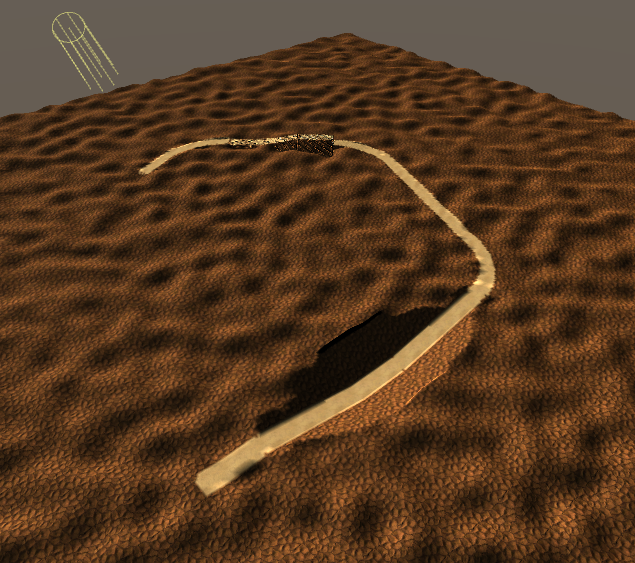
\includegraphics[height=\imgHeightMedium{}]{img/Test_TerrainGeneration.png}}
			\captionof{figure}{Terrain généré à l'aide du script et importé dans \textit{Unity}.}
			\label{TerrainGeneration}
		\end{minipage}\medskip	
		\\
	
		Comme expliqué dans l'introduction de cette sous-section, l'appauvrissement final de la géométrie du terrain est implémenté de façon plus simple. Il consiste en trois fichiers de terrains proposant les trois versions. Le terrain choisit est lié au facteur "Terrain details lvl" du script "ImpoverishmentModel" étant un entier allant de 1 à 3. Le niveau 3 correspond au terrain tel qu'il est dessiné, sans appauvrissement. Les niveaux 1 et 2 sont des versions appauvries (lissées). Chaque niveau possède donc trois objets de terrain différents. Le bon terrain est chargé d'après la valeur de la variable. Le niveau 2 tend à réduire toutes les rugosités et imperfections du terrain. Le niveau 1 essaie au possible de diminuer les différentes hauteurs et de proposer des formes géométriques. Ces terrains se trouvent dans le répertoire "Terrains/WorldX", appelés "TerrainWorldX\_Y" où "X" est le numéro du monde et "Y" la valeur de "Terrain details lvl" correspondante. Cet appauvrissement est visible, pour le monde 1, dans la figure \ref{TerrainGeometryImpoverishment}. On y voit, de gauche à droite, les valeurs d'appauvrissement de 3 à 1. En haut est montrée une vue totale du terrain et en bas, un aperçu depuis le sol.\medskip
		
		\begin{minipage}{\linewidth}
			\makebox[\linewidth]{
				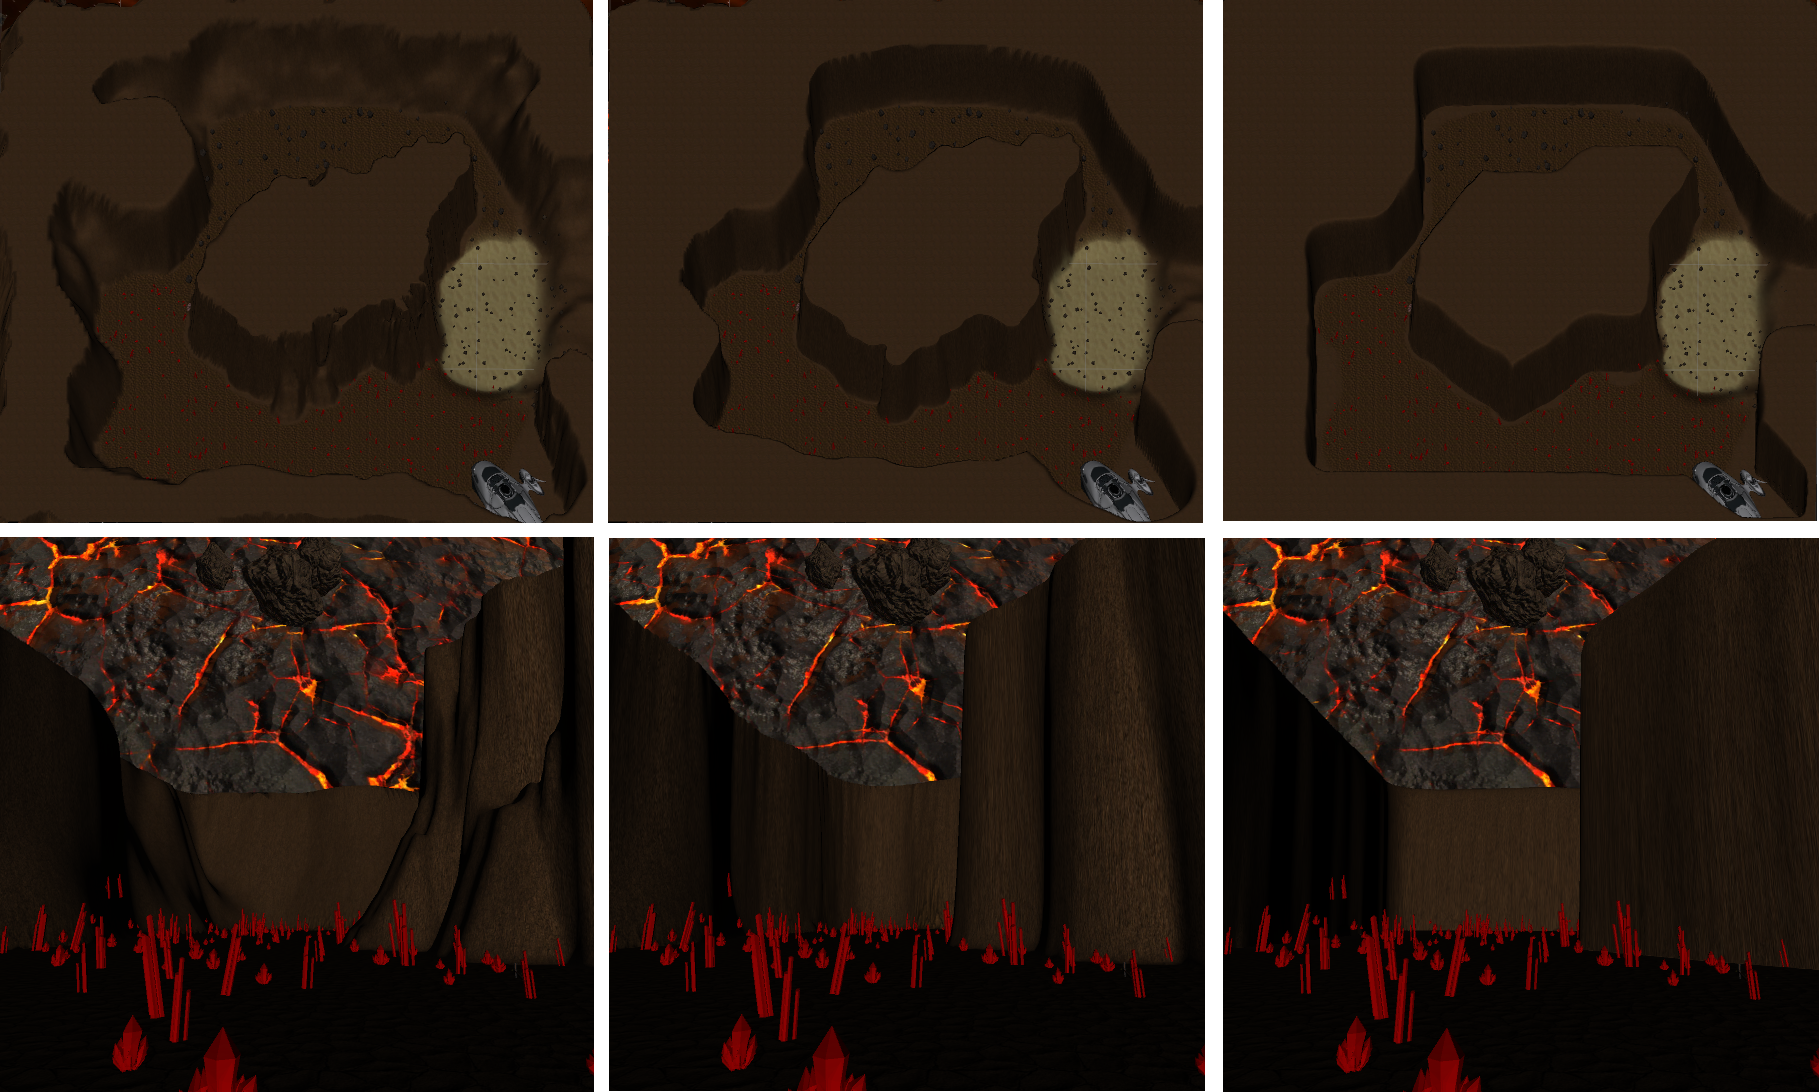
\includegraphics[height=\imgHeightMedium{}]{img/Developpement_GeometryTerrain.png}}
			\captionof{figure}{Appauvrissement du terrain du monde 1.}
			\label{TerrainGeometryImpoverishment}
		\end{minipage}\medskip		
		
	\subsection*{Autres appauvrissements du terrain}
		
		Premièrement, concernant les \textit{landscape elements}, il y a l'appauvrissement quantitatif. Il influe sur le nombre d'objets présents sur le terrain avec un paramètre allant de 0 à 2 ("Quantity factor" du script "ImpoverishmentController"). Le SG n'utilise que ce paramètre de 0 à 1. "0" correspondant à aucun objet et "1" correspond au SG adapté pour une personne ne nécessitant pas d'appauvrissement. La relation entre ce facteur et le nombre d'objets est linéaire. Il permet de monter jusqu'à "2". Cela représente donc deux fois le nombre d'objets considéré comme normal. Cette fonctionnalité, bien que non utilisée actuellement, a été pensée pour permettre de créer des niveaux volontairement plus complexes que la normale. Le réglage du nombre d'objets afin qu'il corresponde au paramètre est effectué par l'activation et la désactivation des objets ayant le script "Landscape elements". Ceux-ci étant dans la structure de \textit{GameObjects} "World, Terrain, TerrainElements, Landscape elements". L'activation de tous correspond à la valeur 2. Leur placement est aléatoire (réalisé par script, voir section \ref{sDevDeroulementPartie}). Le choix des éléments à désactiver ou à activer n'a donc pas d'importance, ils seront toujours répartis de façon cohérente sur le terrain.
		
		La figure \ref{QuantityImpoverishment} montre, de gauche à droite, les valeurs 0, 1, et 2 de cet appauvrissement. La ligne du haut montre une vue possible du SG et celle du bas montre le niveau, vu du dessus.\medskip
		
		\begin{minipage}{\linewidth}
			\makebox[\linewidth]{
				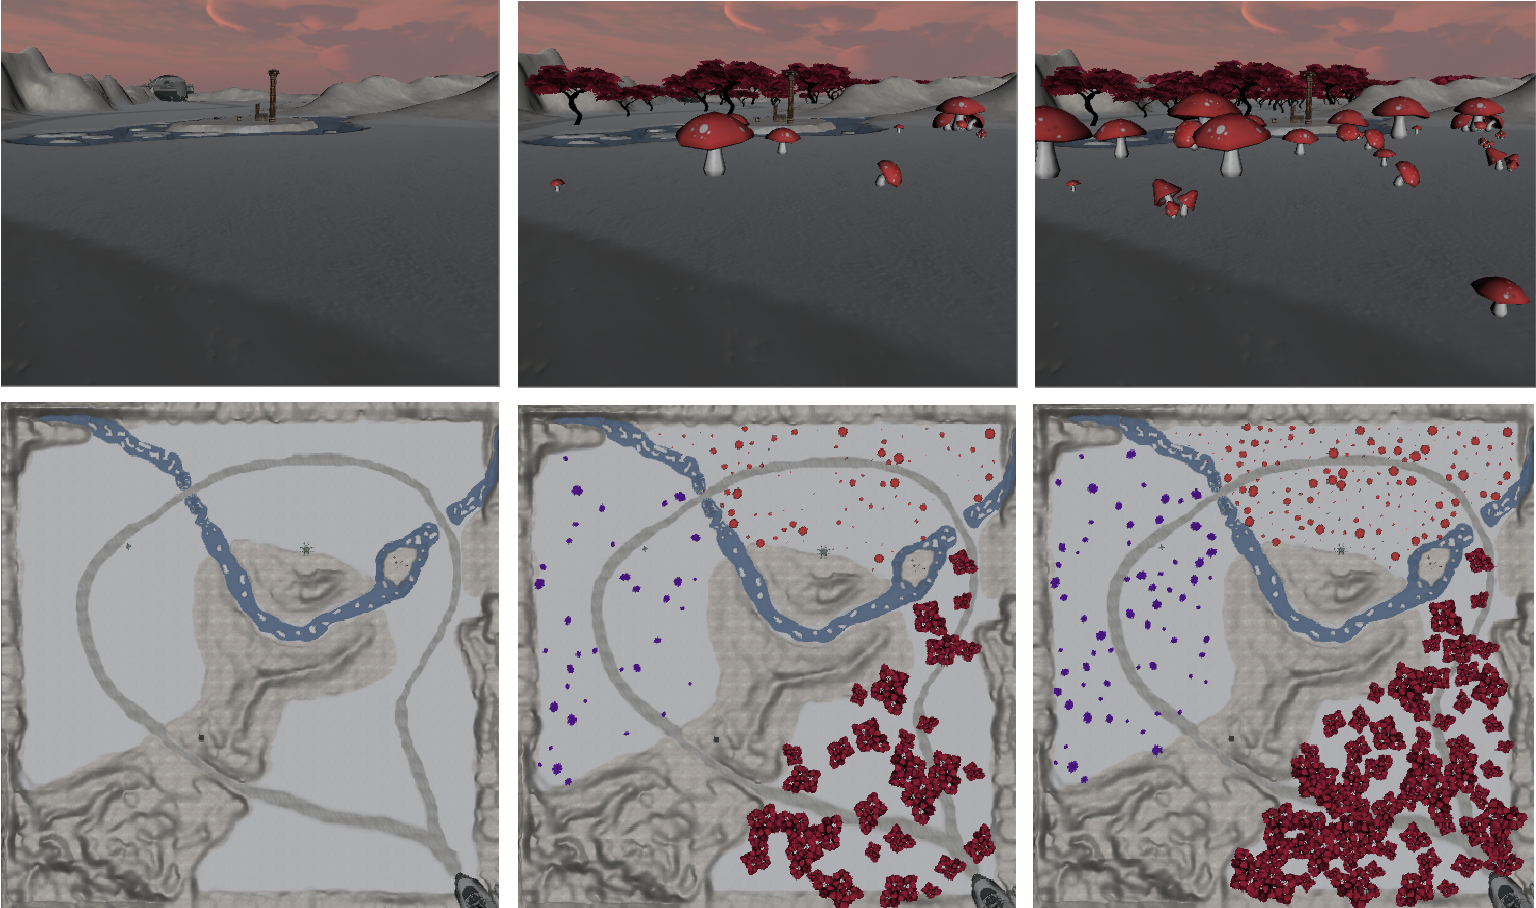
\includegraphics[height=\imgHeightMedium{}]{img/Developpement_DemoQuantity2.png}}
			\captionof{figure}{Visualisation de l'appauvrissement quantitatif. Dans l'ordre, 0; 1; 2.}
			\label{QuantityImpoverishment}
		\end{minipage}\medskip
		\\
		
		Deuxièmement, il y a l'appauvrissement de l'herbe. Celui-ci est lié à un booléen définissant la présence ou non d'herbe. L'herbe est ajoutée manuellement sur les terrains à l'aide de la fonction "Paint details" du terrain \textit{Unity}. Chaque géométrie du terrain doit se faire ajouter de l'herbe. L'herbe n'est pas obligatoire, seule deux mondes sur cinq en contiennent (les mondes 2 et 3). Les caractéristiques de l'herbe sont définies dans l'inspecteur du terrain et accessibles dans son attribut "detailPrototypes". La désactivation de l'herbe utilise des fonctionnalités non documentées de \textit{Unity}. Elle pourrait ne plus fonctionner lors de prochaines versions. L'herbe n'a qu'une valeur décorative. C'est pourquoi une solution concernant son placement de façon automatique n'a pas été envisagée.
		
	\subsection*{Appauvrissement du rendu}
		Plusieurs solutions ont été testées dans une phase de tests concernant cet appauvrissement. La première technique testée consiste à l'utilisation d'une palette de couleurs réduisant ainsi le nombre de couleurs possible à la taille de la palette. Cette taille pouvant être le facteur à influer. Chaque couleur se voit alors remplacée par celle la plus proche dans la palette. Le remplacement se fait en fonction d'un calcul de distance entre couleurs \cite{colorDiff}. L'implémentation réalisée pré-calculait ce remplacement pour chaque couleur possible dans une texture 3D de 256 par 256 par 256 (pixels). Le \textit{shader} n'avait qu'à prendre la valeur à l'indice "rouge", "vert" et "bleu". Le premier désavantage de cette technique est qu'il faut une nouvelle palette pour chaque niveau d'appauvrissement. Le deuxième est qu'il faut créer ces palettes (ce qui, pour être fait correctement, nécessite les compétences d'un \textit{designer}). Le dernier désavantage est qu'il faudrait tout refaire pour chaque niveau. Car ceux-ci peuvent être très différents les uns des autres. Une solution est de générer ces palettes d'après le contenu de la scène. Ceci pourrait être réalisé à l'aide d'un histogramme de notre monde et l'isolation des pics de celui-ci. Cette solution n'a cependant pas été testée et le test de la deuxième technique fut effectué.
		\\
		
		La deuxième technique consiste à régler le nombre de valeurs que peut prendre chaque composante (rouge, vert, bleu) de la couleur. On peut ainsi proposer un grand nombre de valeurs pour cet appauvrissement, allant de 2 à 256. Cette technique est valable pour tous les mondes et n'en complique pas l'ajout. En contrepartie, le résultat est de moindre qualité. Ceci est dû au fait qu'elle supprime progressivement toutes les nuances et ne garde pas forcément les couleurs les plus utiles. Malgré son résultat de moindre qualité, c'est cette technique qui est implémentée dans le SG actuel. Le paramètre du script "ImpoverishmentMode" correspondant est "Nb colors". La raison du choix de la technique a été sa facilité d'application et l'absence de travail supplémentaire pour chaque niveau. Elle est implémentée dans le \textit{shader} "ReduceColor". Son implémentation diminue le nombre de couleurs à l'aide d'une division entière. L'arrondi à l'entier inférieur a pour conséquence, dans les extrêmes, d'assombrir l'image. Un aperçu en jeu, de différentes valeurs d'appauvrissement est présent dans la figure \ref{NbColorImpoverishment}.\medskip
		
		\begin{minipage}{\linewidth}
			\makebox[\linewidth]{
				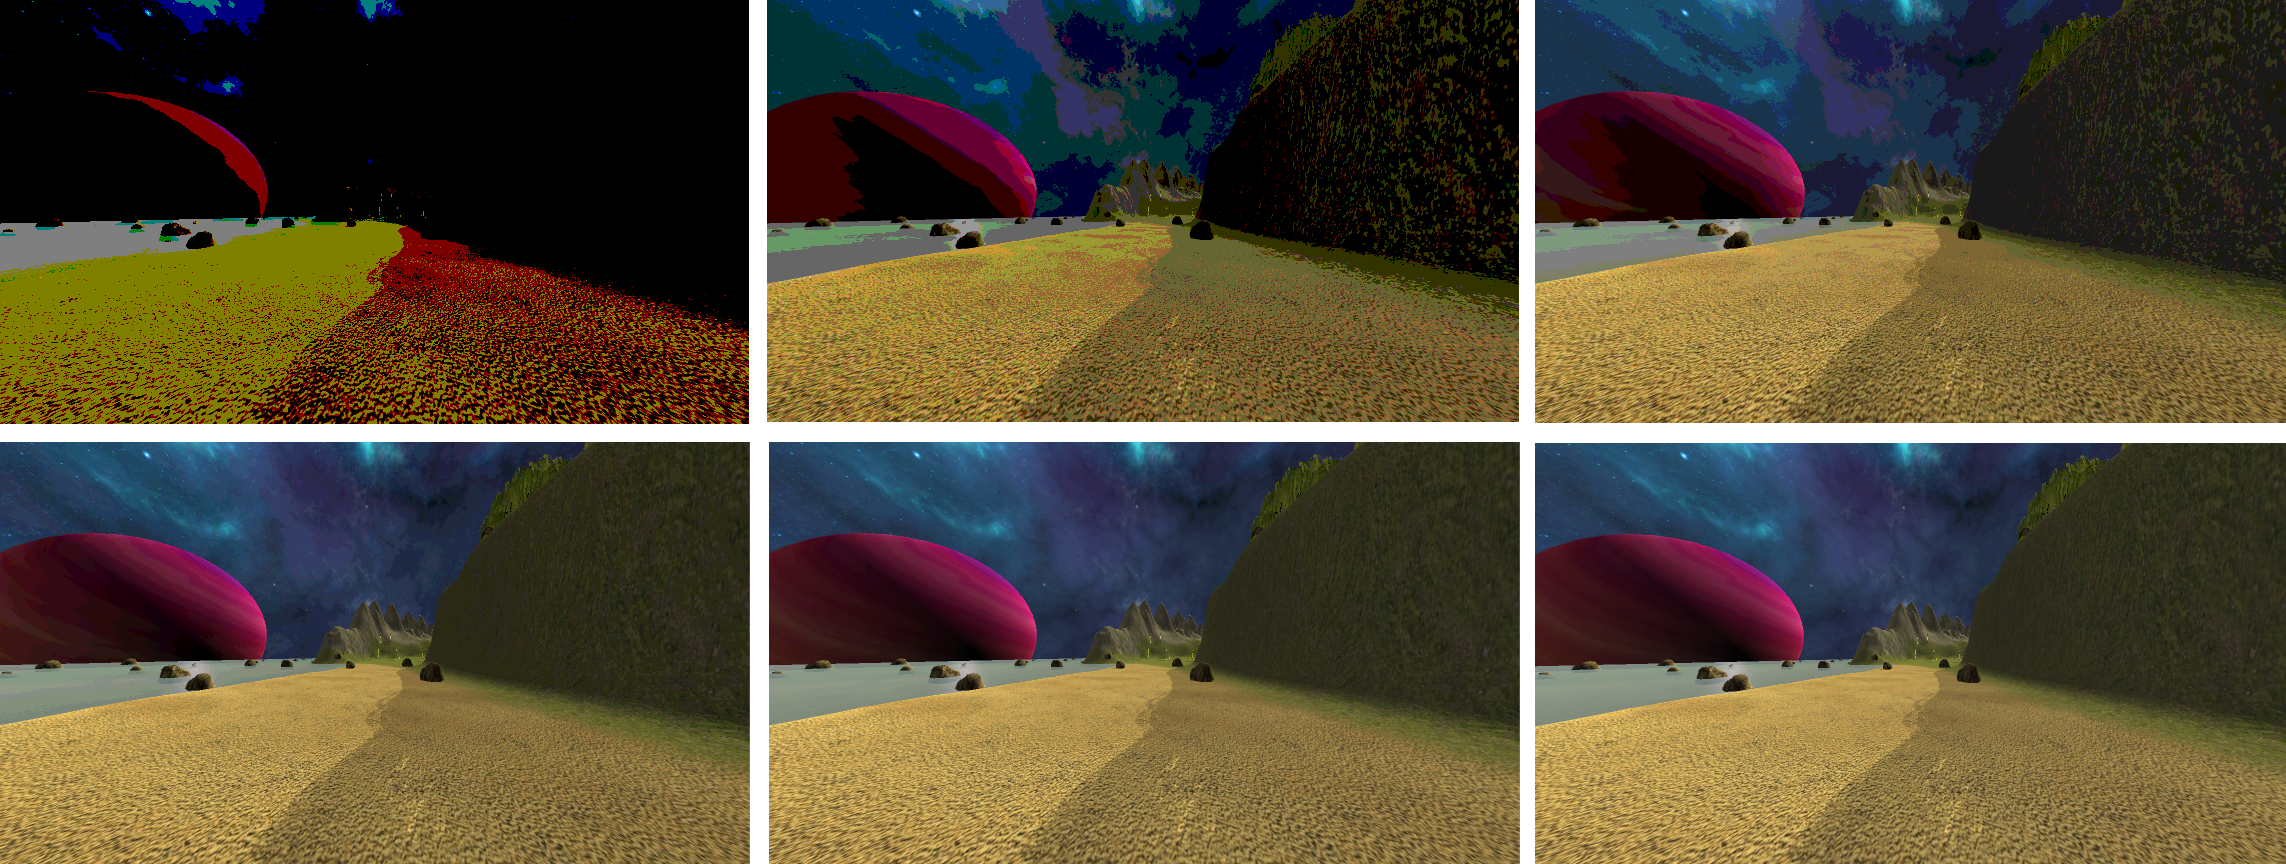
\includegraphics[height=\imgHeightSmall{}]{img/Developpement_AppauvrissementCouleurs.png}}
			\captionof{figure}{Visualisation de l'appauvrissement du nombre de couleurs. Dans l'ordre de lecture, 2; 5; 10; 25; 50; 100.}
			\label{NbColorImpoverishment}
		\end{minipage}\medskip
		\\
		
		Différentes techniques d'applications de ces sélections de couleurs sont possibles. La première est de l'appliquer au rendu. C'est cette technique d'application qui est implémentée dans le SG et qui a permis de produire la figure \ref{NbColorImpoverishment}.
		On y remarque que des zones de couleurs se créent sur l'image, se superposant ou effaçant la géométrie de la scène. Le problème principal vient des effets de lumière, d'ombre et de dégradés.
		Divers essais ont été réalisés pour appauvrir le rendu. Les premiers consistent à rendre de contenu d'une caméra dans une texture, puis la placer dans la scène, devant la caméra principale en lui appliquant le \textit{shader}. Mais la méthode la plus directe et induisant le moins de manipulations, consiste à appliquer le \textit{shader} sur la caméra à l'aide du script "RenderPostProcessEffectViewer".
		\\
		
		Une autre technique d'application consisterait à appliquer le \textit{shader} sur chaque objet de la scène. Cela devrait se faire avant le calcul de lumière, pour être compatible avec l'appauvrissement de la lumière et éviter les problèmes actuels. Un problème vient tout de même s'ajouter: les calculs de lumières vont ajouter des dégradés sur nos objets, les faisant au final utiliser plus de couleurs que la sélection faite. Cette solution peut tout de même permettre un appauvrissement des couleurs adapté au patient. Elle mériterait donc d'être implémentée. Elle n'est pas actuellement implémentée sa charge de travail a été jugée importante. En effet, pour appliquer l'effet sur chaque \textit{material}, il faut probablement modifier chaque \textit{shader} utilisé. C'est pourquoi seule l'application sur le rendu est présente dans le SG actuel.
		
	\subsection*{Appauvrissement sonore}
		Dans le chapitre Conception, section \ref{sConSelectionObjectifs}, plusieurs options ont été proposées. Celle retenue est la classification des sons par famille et la sélection des familles actives. Ce choix est dû aux fichiers audio libres de droits trouvés (liste disponible dans les annexes). Ceux-ci ne permettant pas les solutions plus complexes. Ainsi, quatre familles de sons ont été créées.
		\\
		
		La première, "bruits de pas", est probablement la plus importante du SG car elle donne un retour à l'utilisateur sur sa marche. Elle est également celle ayant demandé le plus de travail et qui est la plus détaillée de ce rapport. Chaque type de sol possède son propre ensemble de bruits de pas. Ceux-ci ayant été extraits de séquences audio de marches sur différents types de sols. Chaque sol contient ainsi plusieurs sons de pas afin d'éviter la monotonie. Un d'entre eux est choisi aléatoirement et lancé quand un pied touche le sol. C'est le LHS qui doit communiquer si le pied touche le sol ou pas, cela grâce aux modèles mathématiques de mouvements qui seront développés dans la suite du projet R\&D. En l'absence du LHS, un simulateur basé sur une animation et des \textit{colliders} est utilisé (plus de détails dans la section \ref{sDevDeroulementPartie}). Le type de sol, dépend du type de segment de parcours effectué (classe "PathSegment"). Pour les segments dans le vaisseau, le même ensemble de bruits de pas est utilisé. Pour le segment sur le terrain, un ensemble de bruit est utilisé selon la texture du terrain. Pour connaître la texture, la \textit{splatmap} du terrain est utilisée, elle représente les différentes textures du terrain (visible dans la figure \ref{TerrainSplatmap}). En fonction de la position du joueur, on calcule les coordonnées correspondantes de la \textit{splatmap} et on peut déduire le type de sol. Les \textit{splatmaps} supportant les dégradés, dans ces situations c'est un son du sol avec la plus haute valeur qui est lancé (en cas d'égalité, la première valeur est conservée, dans l'ordre "rouge", "vert", "bleu").\medskip
		
		\begin{minipage}{\linewidth}
			\makebox[\linewidth]{
				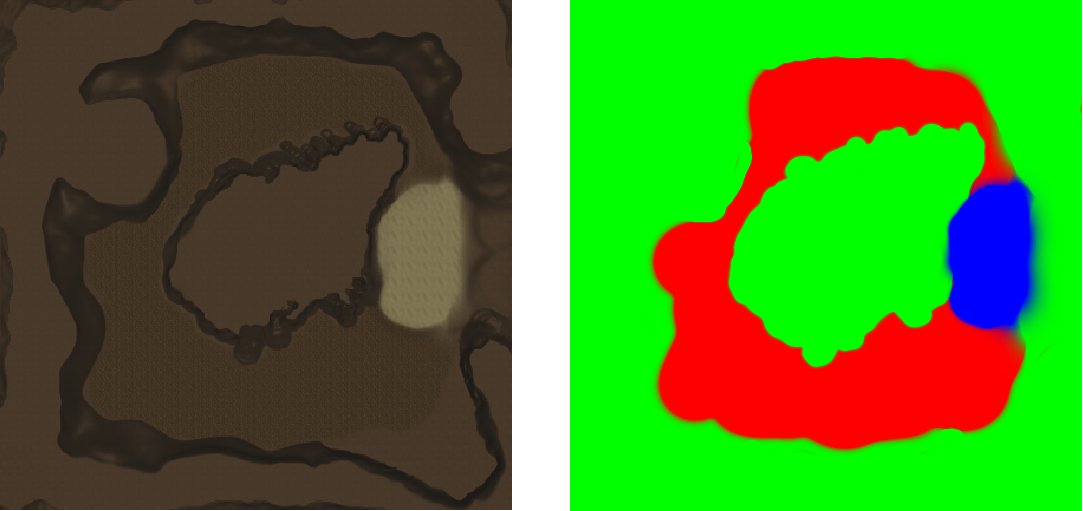
\includegraphics[height=\imgHeightSmall{}]{img/Developpement_TerrainSplatmap.png}}
			\captionof{figure}{Terrain du monde 1 et sa \textit{splatmap}.}
			\label{TerrainSplatmap}
		\end{minipage}\medskip
		
		Des exceptions sont possibles grâce aux éléments placés sur le chemin et possédant le script "PathModifier" (\textit{e.g.}, le pont du monde 2). Ce dernier permet de modifier la hauteur et le son du chemin (et ne pas prendre celui de terrain). La zone modifiée par ce script est définie par un \textit{collider} attaché au \textit{GameObject}. Ce \textit{collider} doit également être dans la couche (\textit{layer}) "HeightModifiers". Plus de détails concernant ce script sont présentés dans la section \ref{sDevDeroulementPartie}. 
		\\
		
		La deuxième famille de sons est celle des sons d'interfaces. Elle comprend un son de succès lorsqu'un objectif est trouvé ainsi que le son de scintillement qu'ils émettent. Ce scintillement a été ajouté par Monsieur K. Laipe. La troisième famille est celle des sons d'ambiance. Elle comprend tous les sons de l'environnement (\textit{e.g.}, bourdonnement de moteur dans le vaisseau, bruit de la cascade, son des vagues, etc.). La dernière famille concerne la musique de fond qui ne commence qu'une fois un niveau chargé et peut varier d'un niveau à l'autre.
		\\
		
		Toutes ces sources audio sont attachées à un \textit{GameObject}. Pour permettre l'appauvrissement, ce dernier doit avoir un \textit{tag} spécifique. Ce \textit{tag} doit valoir "FootStep", "UI", "BackgroundSound" ou "Music" d'après la famille à laquelle il appartient (ces valeurs correspondent aux familles dans l'ordre donné précédemment). Au chargement du SG et à celui d'un niveau, l'ensemble des sources audio sont récupérées et activées/désactivées en fonction de la sélection effectuée dans "ImpoverishmentModel". Toutes les sources audio avec un \textit{tag} ne correspondant pas à ceux précédemment cités sont désactivées. On peut voir le placement de ces sources audio et leur rayon d'émission dans la figure \ref{AudioImpoverishment}. \medskip
		
		\begin{minipage}{\linewidth}
			\makebox[\linewidth]{
				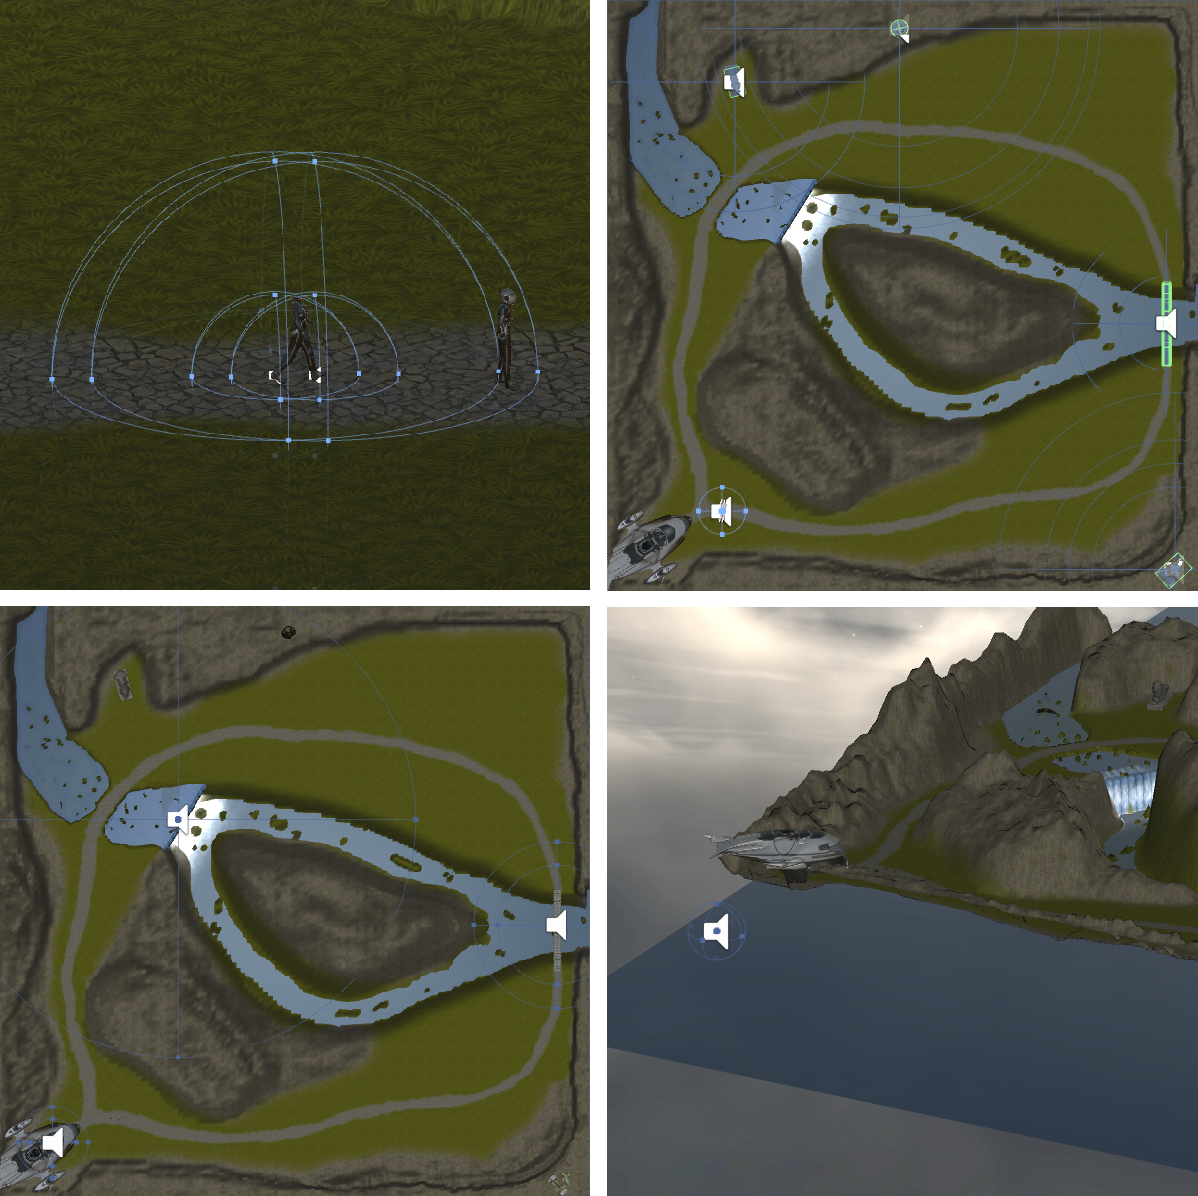
\includegraphics[height=\imgHeightMedium{}]{img/Developpement_AudioImpoverishment.png}}
			\captionof{figure}{Appauvrissement audio - Affichage des sources par famille. Dans l'ordre de lecture: bruits de pas; sons d'interfaces; sons d'ambiance; musique de fond.}
			\label{AudioImpoverishment}
		\end{minipage}\medskip%TODO: Refaire avec un meilleur contraste pour la zone d'émission (sur un autre sol, ou autre technique)
		
		
		Pour permettre une sélection de plusieurs valeurs dans "ImpoverishmentModel", ce dernier ne possède qu'un champ de l'énumération "AudioType\_E". Cette dernière étant composée des valeurs suivantes: MUSIC = 8, BACKGROUND\_SOUNDS = 4, UI\_SOUNDS = 2, FOOTSTEPS = 1. Ce qui correspond aux valeurs binaires 1000, 0100, 0010, 0001. Puis, dans le script "ImpoverishmentModelEditor", on fait correspondre le paramètre "audioTypes" avec un "\textit{EnumMaskField}. Cela permet de pouvoir choisir plusieurs valeurs si l'énumération possède des valeurs permettant une combinaison par "ou" logique. Il propose même des raccourcis pour sélectionner toutes ou aucune des valeurs, comme on le voit sur la figure \ref{AudioEnumMaskField}. Par exemple, la sélection "bruits de pas" et "sons d'ambiance" correspond à la valeur "0101". Pour savoir si un son doit être désactivé, il suffit d'effectuer un "et" logique entre sa valeur d'énumération et le masque et, si le résultat est différent de 0, il faut l'activer.\medskip
		
		\begin{minipage}{\linewidth}
			\makebox[\linewidth]{
				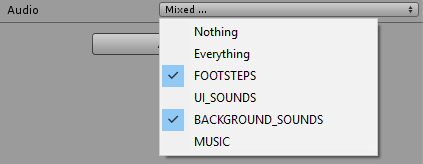
\includegraphics[height=\imgHeightSmall{}]{img/Developpement_EnumMaskfield.png}}
			\captionof{figure}{Sélection de l'appauvrissement audio via un \textit{EnumMaskField}.}
			\label{AudioEnumMaskField}
		\end{minipage}\medskip	
		
	\subsection*{Appauvrissement des effets de lumière}
		Comme définit dans la sélection des objectifs (chapitre Conception, section \ref{sConSelectionObjectifs}), l'appauvrissement des effets de lumière comprend trois valeurs: "uni"; "diffus"; "diffus et spéculaire". Le calcul des effets de lumièress est effectué dans les \textit{shaders} utilisés par les \textit{materials}, eux-mêmes utilisés par les \textit{renderers}. La solution implémentée consiste à considérer le SG dans son état de base comme correspondant à "diffus et spéculaire". Au chargement de chaque scène, on récupère tous les \textit{renderers} de la scène et on construit, pour chaque \textit{materials}, deux autres versions (une pour "diffus" et une pour "uni"). Le script "LightImpoverishmentController" se charge de faire correspondre au \textit{renders} les bons \textit{materials}. Ceci se fait d'après le paramètre "Light" de "ImpoverishementModel". Celui-ci est un entier allant de 0 à 2 (0 = uni; 1 = diffus; 2 = diffus et spéculaire).
		\\
		
		Pour la valeur "diffus", un nouveau \textit{material} est créé pour chaque \textit{material} existant. Ce dernier cependant utilise le même \textit{shader} que le \textit{material} de base. Il met juste les paramètres "\_Glossiness" et "\_Metallic" à 0. Il met également les textures "\_SpecGlossMap" et "\_MetallicGlossMap" à "\textit{null}". Ces dernières correspondent à la \textit{specular map} et la \textit{metallic map} utilisées par les \textit{shader} "Standard" et "Standard (Specular setup)". Cet appauvrissement est compatible avec ces deux shader ainsi que tout autre dont les reflets ne dépendent que d'un ou de plusieurs paramètres dont les noms correspondent (notamment ceux utilisés pour les arbres: "Nature/Tree Creator Bark" et "Nature/Tree Creator Leaves"). Si d'autres viennent à être utilisés ou créés, il faut s'assurer qu'ils possèdent au moins un de ces paramètres et que sa mise à zéro (ou \textit{null}) supprime tous reflets.
		\\
		
		Pour la valeur "uni", un nouveau \textit{material} est également créé pour chaque \textit{material} existant. Ce dernier utilise le script "Custom/Unlit/Texture Colored" ou "Custom/Unlit/PointBillboardGeometryShader", implémentés respectivement dans le fichier "UnlitTextureColored.shader" ou "UnlitPointBillboardGeometryShader.shader" du dossier "Shaders". Le premier est une combinaison des \textit{shaders} "Unlit/Color" et "Unlit/Texture" proposés par \textit{Unity}. Ces derniers permettent d'afficher un modèle avec respectivement, une couleur ou une texture sans aucun effet de lumière. La combinaison permet, comme, par exemple, dans le \textit{shader} "Standard", d'obtenir une texture multipliée par une couleur (utilisé notamment par les rochers du monde 5). Il ajoute également un paramètre, "\textit{Aplha cutoff}". Il agit comme seuil, si la composante "alpha" de la couleur est en dessous, aucune couleur n'est produite. Ce paramètre est utile à tout élément contenant du feuillage. Le deuxième \textit{shader} contient le \textit{geometry shader} permettant la duplication d'un point en quatre et l'orientation face à la caméra. Il est utilisé pour les \textit{billboards} et, contrairement au \textit{shader} habituels de ceux-ci, il ne calcul aucun effet de lumière.
		
		Le \textit{material} est créé comme un clone de l'original, puis le \textit{shader} est changé. Tous les paramètres possédant le même nom récupèrent la valeur de l'ancien \textit{shader}. Aucun réglage supplémentaire n'est nécessaire. Avec cet affichage, il est impossible de distinguer des reliefs sur des surfaces sans textures. C'est pourquoi les pièces intérieures du vaisseau spatial ont des couleurs différentes pour les murs, le sol, le plafond, les portes et leurs pourtours.
		%TODO: être plus spécifiques ? Ajouter la contrainte d'avoir le même nom que alpha cutoff ? Préciser qu'il s'agit du nom du paramètre et non celui affiché dans l'editor (ou du moins pas quand il est en mode normal).
		\\
		
		La figure \ref{LightImpoverishment} montre un aperçu des trois valeurs du paramètre "Light" allant dans l'ordre croissant. En haut, on y voit un palmier, un rocher, un objectif (statue de Lion), le terrain et de l'eau, comme on pourrait la voir dans un niveau. En bas, on y voit l'intérieur du vaisseau ainsi que le guide. On peut remarquer qu'actuellement le terrain ne subit pas d'appauvrissement. Ceci est dut au fait que son \textit{material} n'est pas accessible de la même façon et le \textit{shader} utilisé est plus compliqué, notamment lié à l'utilisation de plusieurs textures et de la \textit{splatmap}. Ceci est une amélioration possible de cet appauvrissement. On remarque cependant que de la colonne trois à la deux, tous les reflets ont disparu et que de la deux à la une, c'est le cas des ombres.\medskip
		
		\begin{minipage}{\linewidth}
			\makebox[\linewidth]{
				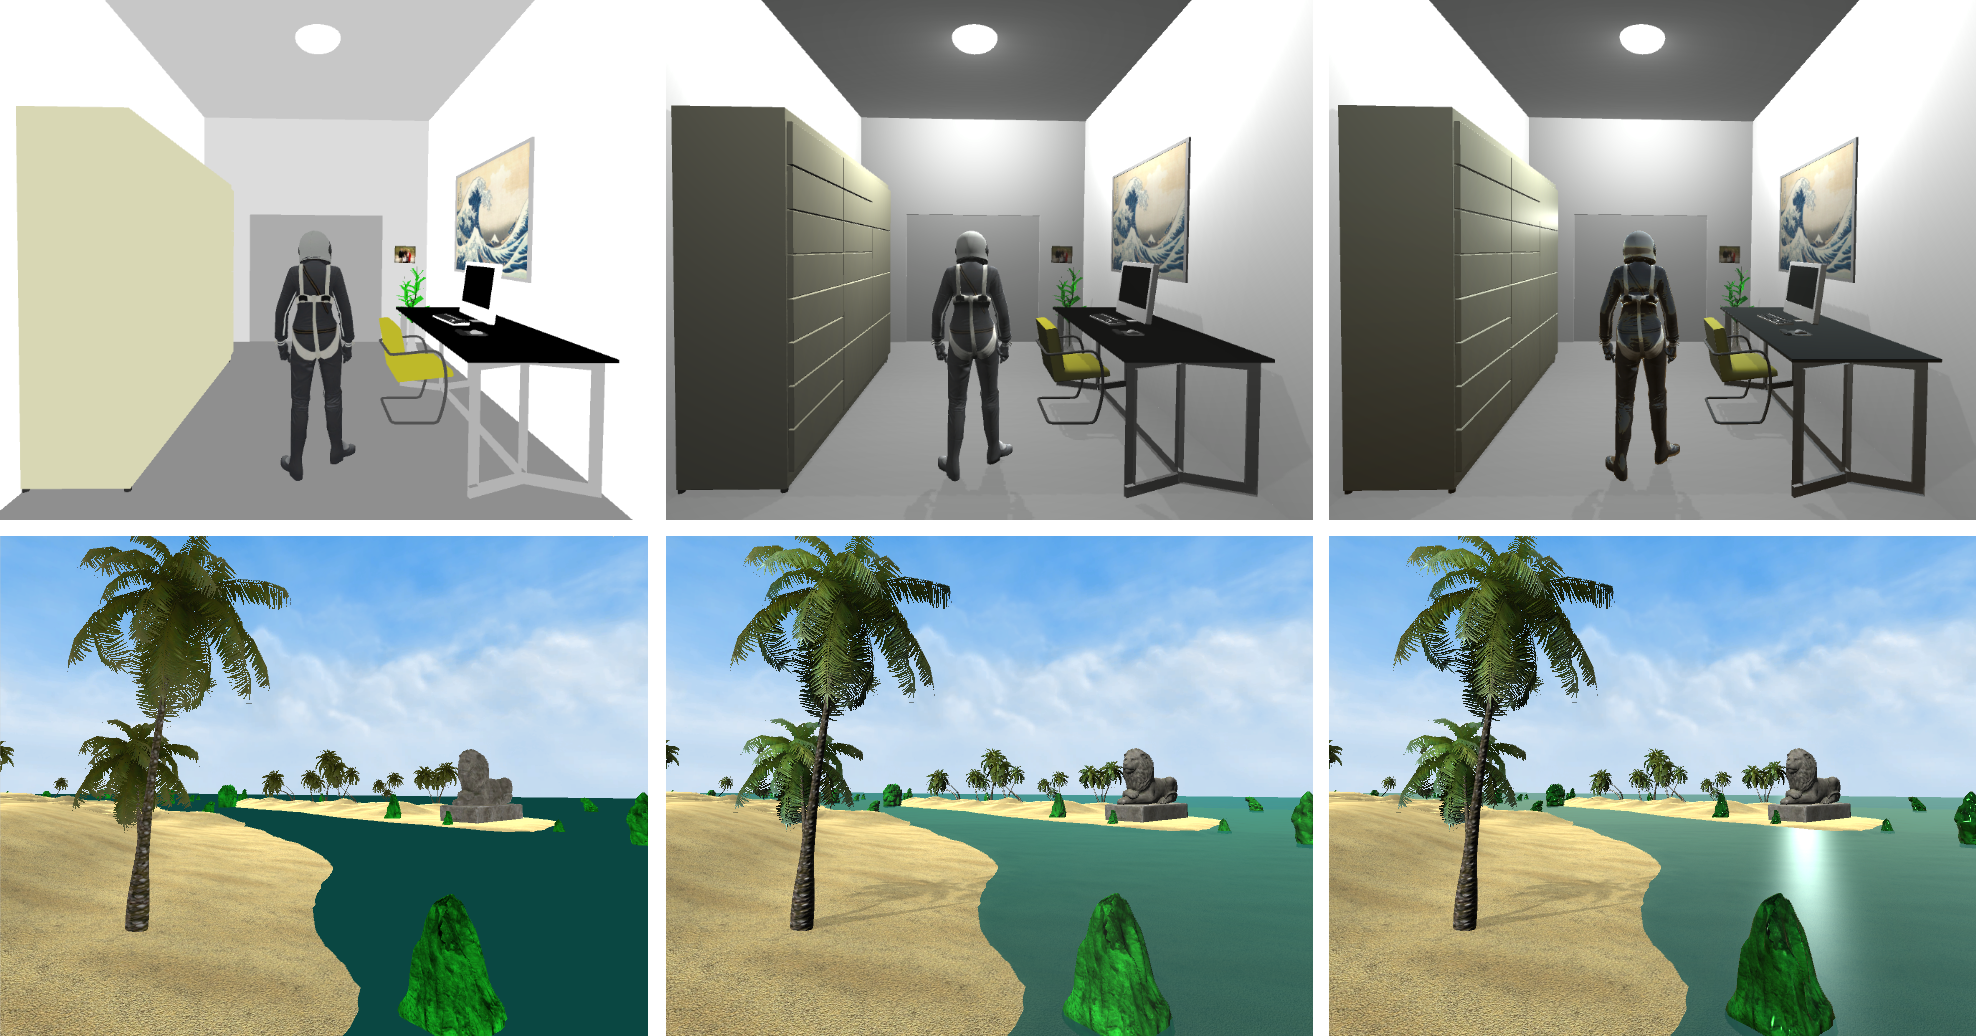
\includegraphics[height=\imgHeightMedium{}]{img/Developpement_LightImpoverishment.png}}
			\captionof{figure}{Appauvrissement des effets de lumière. En haut, aperçu dans le vaisseau et sur le guide. En bas, aperçu durant un niveau.}
			\label{LightImpoverishment}
		\end{minipage}\medskip		
		
	\subsection*{Appauvrissement des animations}
	
		Cet appauvrissement a été implémenté par Monsieur K. Laipe (présenté dans l'introduction de ce chapitre). Cet appauvrissement en regroupe deux: l'appauvrissement des particules et celui des animations. Chacun possède deux valeurs: activé ou désactivé. Ils correspondent aux attributs "Particles" et "Animation" du script "ImpoverishmentController".
		
		L'appauvrissement des particules active ou désactive tous les effets de particule, ce qui comprend: les scintillement des objectifs; l'effet "vapeur d'eau" de la cascade (monde 2); la neige tombante (monde 3). Pour se faire, le script "AnimationController" active ou désactive tous les objets \textit{ParticleSystem}, \textit{ParticleEmitter} et \textit{ParticleRenderer}. Un aperçu des différents éléments avec et sans particules est disponible dans la figure \ref{ParticlesImpoverishment}.\medskip
		
		\begin{minipage}{\linewidth}
			\makebox[\linewidth]{
				\includegraphics[height=\imgHeightMedium{}]{img/Developpement_AppauvrissementAnimation.png}}
			\captionof{figure}{Appauvrissement des particules: en haut: avec; en bas: sans.}
			\label{ParticlesImpoverishment}
		\end{minipage}\medskip	
		\\
		
		L'appauvrissement des animations active et désactive tous les animateurs de la scène qui ne possèdent pas le \textit{tag} "Guide", "Door", "Player" ou "UI". Ces différents animateurs sont essentiels au SG et gèrent, respectivement, la marche du guide, l'ouverture et la fermeture des portes, l'articulation du joueur (quand le SG est joué au clavier) et l'animation de \textit{scan} du HUD. Cela comprend les animations des objectifs telles que celle de l'éolienne. D'autres animations sont effectuées par script. C'est le cas de l'animation des poissons (monde 4 et 5), des palmiers et des vagues (monde 5). Elles n'ont donc pas de composants animateur.	
		\\
			
		Pour permettre leur activation/désactivation gérée par le script "AnimationController", il a été proposé à Monsieur K. Laipe la création d'une interface ("ScriptAnimator\_I"). Elle contient la signature d'une méthode pour l'activation et la désactivation de l'animation. "AnimationController" doit alors, en plus de tous les animateurs (\textit{Animator}), récupérer tous les éléments implémentant l'interface "ScriptAnimator\_I".
		
		Un méthode pour la récupération des tous les éléments implémentant une interface est à disposition dans la classe parente à tous scripts accrochés à un \textit{GameObject} de ce projet: "SGMonoBehaviour". Plus de détails sur cette classe sont présents dans la section \ref{sDevStructure}.	
		
		Finalement, la désactivation des animations supprime également l'effet de vent dans l'herbe.
		
	\subsection*{Paramètre d'appauvrissement général}
		Tous les appauvrissements précédemment décrits dans cette section offrent une grande possibilité de personnalisation du SG pour chaque patient. Cependant, pour l'intégration avec le LHS, il est souhaitable de n'avoir qu'un seul facteur. Ainsi le thérapeute a accès à une seule variable générale pour l'appauvrissement et n'a pas à effectuer tous ces réglages. Ceci est également plus agréable pour l'IHM si le nombre de facteur est diminué. Pour se faire, un paramètre d'appauvrissement général nommé "General impoverishment" est présent dans l'inspecteur du script "ImpoverishmentModel". Il assigne des valeurs à tous les autres paramètres. Ce paramètre va de 1 à 6. Pour chacune de ces valeurs, une sélection des valeurs de chaque paramètre d'appauvrissement est effectuée. Cette sélection est détaillée dans le tableau \ref{tableGeneralImpoverishment}.\medskip
		
		\begin{minipage}{\linewidth}
			\begin{tabular}{|l|c|c|c|c|c|c|}
				\hline
				Appauvrissement&	1&	2&	3&	4&	5&	6 \\
				général&	&	&	&	& &	\\
				\hline
				
				Géométrie des& Primitives&	\textit{Billboard}&	\textit{Billboards}&	\textit{Billboards}&	Géométrie	&	Géométrie \\
				\textit{Landscape} & 3D& &	\textit{Cloud}&	\textit{Cloud}&	complète	&	complète \\
				\textit{elements}& & & & & & \\
				\hline
				
				Géométrie&		1&	1&	2&	2&	3&	3 \\
				du terrain& & & & & & \\
				\hline
				Facteur de&		0.1&	0.3&	0.45&	0.6&	0.8&	1 \\
				quantité& & & & & & \\
				\hline
				Herbe&		\textsf{X}&	\textsf{X}&	\textsf{X}&	\textsf{X}&	\textsf{X}&	\checkmark \\
				\hline
				Animations&		\textsf{X}&	\textsf{X}&	\textsf{X}&	\textsf{X}&	\textsf{X}&	\checkmark \\
				\hline
				Particules&		\textsf{X}&	\textsf{X}&	\checkmark&	\checkmark&	\checkmark&	\checkmark \\
				\hline
				Audio&		\textsf{X}&	\textit{footsteps}&	\textit{footsteps}&	\textit{footsteps}&	Tous&	Tous \\
				&		&	& \textit{UI\_sounds}& \textit{UI\_sounds}&	&	\\
				&		&	&	&	\textit{music}&	&	\\
				\hline
				
				Lumière&		0&	1&	1&	2&	2&	2 \\
				\hline
				Nombre de &		256&	256&	256&	256&	256&	256 \\
				couleurs& & & & & & \\
				\hline
			\end{tabular}
			\captionof{table}{Réglages de l'appauvrissement d'après le paramètre général.}
			\label{tableGeneralImpoverishment}	
		\end{minipage}\medskip
		
		Ces valeurs sont choisies arbitrairement afin d'utiliser les différents aspects de l'appauvrissement. Leur sélection n'a pas été faîte suite à des tests avec le domaine médical. Elle a une valeur démonstrative et ne garantit pas d'avoir une évolution cohérente de la complexité d'interprétation de la scène pour les patients. Ce travail de sélection basé sur une réflexion en collaboration avec le domaine médicale dépasse des objectifs sélectionnés. Il pourra être réalisé dans le projet R\&D englobant.
		
		"Billb." et "Billb.C." désignent les géométrie \textit{billboard} et \textit{billboards cloud} avec normales. Les versions sans normales ne sont pas utilisées, pour que les variation d'effets de lumières ne se fassent qu'avec l'appauvrissement concerné et non la géométrie.
		
		Un aperçu des six niveaux est visible dans la figure \ref{GeneralImpoverishment}.\medskip
		
		\begin{minipage}{\linewidth}
			\makebox[\linewidth]{
				\includegraphics[width=\textwidth]{img/Poster_Appauvrissement3.png}}
			\captionof{figure}{Appauvrissement général. Dans l'ordre de lecture, de 6 à 1.}
			\label{GeneralImpoverishment}
		\end{minipage}\medskip%TODO: Refaire en vertical

\section{Éléments du SG}
	\label{sDevDeroulementPartie}
	
	Dans cette section est détaillée la façon dont sont implémentés les différents composants du SG permettant le déroulement d'un partie. Ce déroulement est également décrit dans les sous-sections concernées. L'élément principal permettant la gestion d'une partie est le script "GameController". Ce dernier est chargé en même temps qu'un niveau. Il définit notamment sa durée, grâce à son paramètre "Time Exercice Minutes". C'est lui qui gère les différents états du SG qui sont: ENTER\_ANIMATION; WAIT\_IOCONTROLLER; PLAY; PAUSE; GAME\_OVER.
	
	\subsection*{Interaction}
		Le SG contient trois interactions: le déplacement; la pause; le \textit{scan}. Pour la première, une section entière lui est consacrée (section \ref{sDevArticulation}). La deuxième existe simplement à des fins de tests, quand le LHS n'est pas disponible. La pause est normalement lancée depuis l'IHM par le thérapeute et ne concerne pas le joueur. Pour le moment, la pause peut être activée et désactivée via un appui sur la touche "P" du clavier. Aucun message ou indication n'est donné au patient, il ne peut juste plus avancer ou scanner. Son implémentation se trouve dans le script "GameController": le temps est figé et l'état passe en "PAUSE". La suite de cette sous-section détaille l'interaction du \textit{scan}.
		\\
		
		Le \textit{scan} est le moyen de valider les objectifs présents dans la scène. Un des avantages est que cela n'ajoute pas de périphérique supplémentaire, tout peut se faire avec le HMD déjà utilisé pour l'immersion. Son deuxième avantage est qu'elle correspond à une interaction naturelle qui est de regarder autour de son environnement. C'est donc probablement une des premières tâches que le patient peut accomplir en même temps que de réaliser son mouvement. Le seul élément non naturel de cette interaction est, une fois l'élément découvert, de devoir le fixer du regard jusqu'à ce que le \textit{scan} soit terminé. Cette opération dure actuellement cinq secondes mais peut être augmenté ou diminué si nécessaire.
		\\
		
		Cette interaction est implémentée à l'aide d'un lancé de rayon partant du centre de la caméra. Il est effectué dans la classe "ScannerController". Ce lancé permet de récupérer le premier \textit{collider} rencontré. Le lancé de rayon lance un \textit{scan} si le \textit{collider} rencontré est dans la couche (\textit{layer}) "Scannable". Pour qu'un élément puisse faire l'objet d'un \textit{scan}, il doit donc avoir un \textit{collider} avec la case "Is Trigger" cochée et être dans la couche "Scannable".
	
		Une fois le \textit{scan} effectué, si l'élément est un objectif, il sera alors considéré comme obtenu. Ce qui a pour conséquence la désactivation des indications d'aides (zone sur la carte et scintillement), l'indication de sa position sur la carte avec un point précis en vert ainsi que la sauvegarde persistante de l'obtention de cet objectif. Ensuite, un aperçu de cet objet s'affiche dans le HUD (voir figure \ref{GuideScan}). Cet affichage permet de visualiser l'objet dans son ensemble. En effet, pour ajouter du challenge, seuls certains éléments d'un objet peuvent être visibles. Cet affichage permet alors de réaliser ce que représente cet objet. Cette affichage dure tant que l'on regarde l'objet. Dès que l'on en détourne le regard, il disparaît progressivement. En regardant à nouveau cet objet et si aucun \textit{scan} n'a été effectué entre temps, il s'affiche progressivement sans réaliser de nouveau \textit{scan}. Cet affichage réalise, par défaut, une rotation constante de l'objet autour de l'axe y pour le voir sous plusieurs angles. Celui-ci peut être désactivé d'un objet à l'autre. Dans le SG actuel, il n'y a pas uniquement les objectifs qui peuvent être la cible du \textit{scan}. Le guide peut également l'être (figure \ref{GuideScan}). Dans ce cas, seules ses jambes sont affichées avec une vue latérale et sans rotation. Cela a pour but de permettre à l'utilisateur de se concentrer sur le mouvement et de le voir sous plusieurs angles afin d'améliorer l'activation des neurones miroirs.\medskip
		
		\begin{minipage}{\linewidth}
			\makebox[\linewidth]{
				\includegraphics[width=\textwidth]{img/Developpement_ScanGuide.png}}
			\captionof{figure}{Animation de \textit{scan} et affichage de l'objet ciblé. Dans l'ordre de lecture: ciblage de l'objet; début du scan; scan en cours; affichage des jambes; jambes en mouvement; disparition de l'affichage.}
			\label{GuideScan}
		\end{minipage}\medskip%TODO: Diminuer taille image. Mieux la décrire (surtout l'animation du scan)
		\\
		
		Chaque objet pouvant être la cible de \textit{scan} doit également posséder le script "ScannableObject". Les paramètres de ce script permettent de régler: la taille de l'objet, pour que la visualisation dans l'affiche correctement; un décalage, pour permettre de mettre l'accent sur certaines zone de l'objet; l'activation de la rotation de la caméra. Les objectifs doivent posséder le script "ObjectiveScannable" héritant de celui cité précédemment. Il permet de considérer l'objet comme un objectif et active par défaut la rotation. Cette visualisation de l'objet est réalisée à l'aide d'une caméra supplémentaire nommée "ScanDetailsCamera". Elle se trouve à la racine de la scène de sélection des niveaux. Son contenu est rendu dans une texture qui est à son tour affichée dans l'aperçu de l'objet. C'est la caméra qui tourne autour de l'objet pour effectuer la rotation. Elle ne rend que les objets étant dans la couche "Scanned". C'est le script "ScannerController" qui s'occupe de placer l'objet cible du \textit{scan} dans cette couche.
		\\
		
		Il est possible de bouger la caméra à l'aide de la souris. Ceci permet le développement du SG sans avoir une disponibilité constante du HMD. Pour cela, il suffit de d'activer le \textit{GameObjet} "WithoutOculus" se trouvant dans celui nommé "IO" à la racine de la scène de sélection des niveaux. Attention à bien le désactiver quand le HMD est utilisé.
		\\
		
		Un dernier aspect est lié à la réalisation de cette interaction: l'animation de l'avatar. Pour améliorer l'immersion et renforcer la cohérence, il est souhaitable que l'avatar s'articule de façon à regarder dans la même direction que la caméra.
		De plus, il est souhaitable que le patient puisse, en regardant vers le bas, voir ses jambes (celles de l'avatar). Cela implique d'appliquer des rotations aux différentes articulations de l'avatar, en partant du bas du dos jusqu'au cou. Ceci a été réalisé dans le script "BodyLookOrientationController" attaché au joueur. Ce dernier nécessite une référence pour l'articulation du cou ainsi qu'un tableau de références pour la colonne vertébrale (figure \ref{AvatarArticulationLook}). Cela a pour but d'être compatible avec plusieurs avatars articulés de différentes façons. La rotation nécessaire est alors divisée sur ces différentes articulations de la façon suivante: chaque partie "i" de la colonne vertébrale a un poids de "i" et le cou a un poids de 2*n; où "n" est le nombre de segments de la colonne et "i" allant de 1 (bas du dos) à "n" (haut du dos). %TODO: Mettre en forme cette "équation"
		Ceci amène à une rotation principalement effectuée au niveau du cou mais tout de même accompagnée par la colonne vertébrale. Cette répartition a été faite de façon expérimentale avec le modèle ayant quatre segments pour la colonne vertébrale. Une fois la rotation appliquée, si celle-ci ne tourne pas uniquement autour de l'axe "y", l'emplacement des yeux ne correspond plus à celui de la caméra. Celle-ci est donc déplacée de façon à correspondre. Si l'articulation de l'avatar ne se fait pas de façon naturelle, ce déplacement pourrait induire un malaise suite à des mouvements rapides et répétés.
		\medskip
		
		\begin{minipage}{\linewidth}
			\makebox[\linewidth]{
				\includegraphics[height=\imgHeightMedium{}]{img/Developpement_ArticulationRegard_Contrast.png}}
			\captionof{figure}{Articulation de l'avatar d'après le regard.}
			\label{AvatarArticulationLook}
		\end{minipage}\medskip	
		
		
		Pour améliorer cette position, l'utilisation du traqueur de position fournit avec l'\textit{Oculus Rift} a été envisagée. Celui-ci induisait cependant une difficulté supplémentaire par rapport à l'articulation. On devait alors faire correspondre non seulement l'orientation mais également la position. Pour cela, il faudrait résoudre des problèmes de cinématique inverse de complexité grandement supérieure \cite{wikipedia_cinematiqueInverse, Buss_InverseKinematicIntro}. D'autre problèmes se posent également avec l'utilisation de ce traqueur, notamment son installation avec le LHS ou encore son comportement hors limite du capteurs (de brusques sauts sont présents par défaut). Pour ces différentes raisons, il a été décidé de ne pas l'utiliser et de se contenter du déplacement induit par les articulations du dos et du cou.
		
	\subsection*{Zone familière}
		La zone familière a été réalisée à l'intérieur du vaisseau spatial. Ce dernier est choisi car il possède une longue zone plate au niveau du terrain. Cet aspect est idéal pour y placer des salles permettant de rejoindre la sortie du vaisseau sans pente ni escalier. Pour l'ouverture du vaisseau, elle se fait à l'aide d'une rotation de la dernière porte, visible dans la figure \ref{Spaceship}. Le modèle 3D du vaisseau a été grossièrement coupé pour permettre une cohérence avec la porte.
		\medskip
		
		\begin{minipage}{\linewidth}
			\makebox[\linewidth]{
				\includegraphics[height=\imgHeightSmall{}]{img/Developpement_Spaceship_Contrast.png}}
			\captionof{figure}{Vaisseau spatial et ouverture de la porte frontale.}
			\label{Spaceship}
		\end{minipage}\medskip
		
		Les murs et les portes des pièces intérieures sont entièrement réalisés à l'aide de primitives 3D disponibles dans \textit{Unity}. La création de ces pièces sur un logiciel de modélisation 3D serait souhaitable mais requiert les compétences d'un \textit{designer}. Cette zone (visible dans la figure \ref{Interior}) est constituée de trois pièces: sélection du niveau; chambre; sas. Elle contient également trois portes menant d'une zone à la suivante. L'éclairage consiste en une lumière ponctuelle par pièce. Cette lumière n'éclaire pas les objets dans la couche "Terrain" ni ceux dans celle "Default". La première pièce est celle de départ et de fin de niveau. Elle contient un écran utilisé pour la sélection du niveau (contre la porte) et un autre écran pour l'affichage du score (contre le mur). La deuxième pièce contient différents éléments familiers faisant le lien entre l'environnement hospitalier et l'environnement étranger des planètes inconnues. Les objets familiers sont les suivants: une armoire; un bureau; une fausse plante; un tableau; une photo de famille. La dernière pièce est un couloir vide donnant accès, une fois la porte ouverte, sur le monde choisit.\medskip
		
		\begin{minipage}{\linewidth}
			\makebox[\linewidth]{
				\includegraphics[height=\imgHeightMedium{}]{img/Developpment_Interior_Detoured.png}}
			\captionof{figure}{Zone intérieure, composée des trois pièces. De droite à gauche: sélection des niveaux; chambre; sas.}
			\label{Interior}
		\end{minipage}\medskip
		\\
		
		Durant une partie, le joueur doit d'abord choisir un niveau (interaction et transition détaillée dans la section \ref{sDevStructure}). Une fois la scène chargée, le SG est dans l'état "ENTER\_ANIMATION". Puis, le vaisseau atterrit puis il passe dans l'état "PLAY", excepté si le LHS n'est pas prêt, où il passe dans l'état "WAIT\_IOCONTROLLER" en attendant. Une fois dans l'état "PLAY", la porte s'ouvre, le joueur peut avancer, rejoindre le guide dans la pièce suivante et réaliser tout le parcours.		
		
	\subsection*{Parcours}
		Pour être guidé sur le parcours, le joueur et le guide contiennent chacun un objet "PathBrowser". Ces objets leur donnent leur déplacements effectué depuis le dernier appel. Ces déplacements sont donnés par une position et une orientation. Celles-ci sont définies dans l'objet "Path" composé d'un tableau de "PathSegment". Durant une partie, c'est une instance de "PathLevel" qui est créée. Celle-ci définit trois segments. Le premier permet d'aller du point "LevelSelectionPoint" à "MainGatePoint" (dans le vaisseau spatial). Le deuxième segment est celui du terrain. Et le troisième est l'inverse du premier, permettant d'aller de l'entrée du vaisseau au tableau des scores. Cette structure de classe est détaillée dans la figure \ref{PathClassDiagram}.\medskip
		
		\begin{minipage}{\linewidth}
			\makebox[\linewidth]{
				\includegraphics[height=\imgHeightMedium{}]{img/Developpement_PathClassDiagram_Resized.png}}
			\captionof{figure}{Diagramme de classes UML des classes utilisées pour la gestion du chemin}
			\label{PathClassDiagram}
		\end{minipage}\medskip%TODO: Mettre en annexe
		
		En début de partie, le vaisseau atterrit de manière à s'aligner avec le début du parcours. La transition entre le premier et le deuxième segment est donc assurément fluide. Pour que la transition entre le deuxième et le troisième soit également fluide, il faut s'assurer que le tracé du terrain donne la même orientation initiale que finale (bien que tournée de 180°). Ce tracé est fait dans un fichier ".svg" (étant un fichier de type XML) à l'aide du logiciel de dessin vectoriel "\textit{Inkscape}" \cite{Inkscape_website}. 		
		Une fois le tracé dessiné (contraintes expliquées plus bas dans cette sous-section), deux étapes sont à effectuer. Le dessin est exporté en bitmap au nom de "PathmapWorldX.png" et le fichier de dessin (.svg) est renommé en "path\_WorldX.xml" (pour pouvoir être importé par \textit{Unity} comme \textit{text asset}). Ces deux fichiers sont placés dans le répertoire "Terrain" et référencés dans l'objet préfabriqué "LevelX". Le fichier bitmap est affiché sur la carte quand le niveau est chargé. Le fichier XML subit plus de traitements, pour finalement projeter le tracé sur le relief du terrain. Ces traitements consistes à extraire les différents points de la courbes et leur points de contrôle et de discrétiser ces courbes d'après l'équation des courbes de Bézier cubiques \cite{CompAlg} (équation utilisée pour leur dessin). Chaque segment est alors discrétisé en 100 points et 100 directions. La raison de cette discrétisation est que l'équation donnant la position d'après le chemin parcouru (nécessaire au SG) est de complexité bien supérieure. Ce traitement est effectué dans la classe "SVGTools". La projection, bien que visible sur tous les mondes, est mieux illustrée sur le monde 1 car c'est le seul monde avec des pentes sur le chemin. Cette visualisation du chemin (figure \ref{PathInGizmos}), est visible uniquement dans l'éditeur de scène "\textit{Gizmos}", grâce au script "DrawPath". Les points et directions sont stockés dans l'instance de "PathSegmentTerrain". L'interpolation entre ces points et directions est linéaire et est réalisée par l'instance de "Path".\medskip
		
		\begin{minipage}{\linewidth}
			\makebox[\linewidth]{
				\includegraphics[height=\imgHeightSmall{}]{img/Developpement_CheminTrace.png}}
			\captionof{figure}{Tracé du chemin, tel qu'il est perçu dans \textit{Gizmos}.}
			\label{PathInGizmos}
		\end{minipage}\medskip
		
		Le dessin du chemin peut être réalisé avant ou après la création du terrain. Dans les deux cas, des contraintes doivent être respectées. Premièrement, le chemin doit être effectué en une seule courbe de Bézier. Deuxièmement, le chemin doit boucler en un point (le point final étant au même emplacement que le point de départ). Le point de contrôle du point initial et du le point final doivent être sur une même droite, du même côté du point (initial et final). Troisièmement, chaque autre point de la courbe doit avoir deux points de contrôles. Le point et ses points de contrôle doivent être sur une même droite, ces deux derniers étant chacun d'un autre côté du point (option "rendre doux les nœuds sélectionnés"). Ceci se vérifie visuellement sur la figure \ref{PathDrawing}. On y voit chaque point (autre que l'initial et le final) représenté par un carré. Finalement, le fichier de dessin doit être de 512 sur 512 (pixels). Cette page représente le terrain, il est donc souhaitable que la courbe tracé ne s'approche pas des bords. Le point initial doit également veiller à laisser suffisamment de place derrière lui pour que le vaisseau spatial soit bien intégré au terrain. Sans être une contrainte fonctionnelle, il est préférable d'avoir un chemin assez lisse et d'éviter les virages trop serrés. Ainsi le changement d'orientation automatique est plus doux pour le joueur et diminue le risque de nausées.%TODO: Retrouver une ref.
		\medskip
		
		\begin{minipage}{\linewidth}
			\makebox[\linewidth]{
				\includegraphics[height=\imgHeightSmall{}]{img/Developpement_DessinChemin.png}}
			\captionof{figure}{Aperçu du tracé sous \textit{Inkscape}. Dans l'ordre de lecture: sur fond blanc; sur une capture d'écran; sur la \textit{splatmap}.}
			\label{PathDrawing}
		\end{minipage}\medskip
		
		Si ce tracé est dessiné avant que le terrain soit créé, on peut alors modéliser le terrain autour de ce chemin dans l'éditeur. Il faut faire attention à minimiser les pentes ou à les rendre lisses, même si elles n'ont aucune influence sur l'exercice pour le moment. Si ce tracé est réalisé après le terrain, il peut être dessiné sur une capture d'écran du terrain ou sa \textit{splatmap}. Cette dernière peut être récupérée en sélectionnant le \textit{GameObject} possédant le terrain, puis en effectuant l'action "NWTools, Terrain, Export Splatmap". Elle est créée dans le dossier "Assets" au nom "splatmap.png". Les trois possibilités sont montrées dans la figure \ref{PathDrawing}.
		\\
		
		Comme le montre le diagramme de classe (figure \ref{PathClassDiagram}), chaque segment définit un objet sol (script "Ground") qui est responsable du son à lancer lors d'un pas sur ce segment. Il a également été expliqué que les hauteurs ne pouvaient pas être données et que celles du terrain étaient utilisées. Or, une autre possibilité existe pour modifier un ou deux de ces aspects. Celle-ci est utilisée pour le pont du monde 2. On remarque qu'on ne suit pas la hauteur du terrain et que les bruits de pas ne sont plus les mêmes. Ceci est possible grâce aux "PathModifier". Tout objet placé sur le chemin et modifiant la hauteur ou le son possède ce script. Il doit aussi contenir un \textit{collider} définissant sa zone. Ce dernier doit être dans la couche "HeightModifiers".
		Une fois le chemin discrétisé et projeté, une étape supplémentaire est réalisée. Pour chaque point, un lancé de rayon est effectué. Le rayon est lancé depuis les coordonné x et z du point ainsi que la hauteur maximum possible du terrain en y. Il est lancé en direction du point. S'il touche un \textit{collider} dans la couche "HeightModifiers" avant de toucher le sol, ce point prend pour hauteur celle du script "PathModifier" attaché à son \textit{GameObjet} ainsi que son objet "Ground".
		
		%TODO: Parler avec plus de détails du calcul des splines
	
	\subsection*{Placement des éléments du jeu}
		Différents éléments du SG se placent dynamiquement d'après un potentiel profil du patient. Celui-ci est à définir dans "PatientProfileModel". On peut y choisir de quel côté placer la carte, l'aperçu des objectifs et la répartition gauche/droite des objectifs. Le choix du côté est directement lié à l'héminégligence du patient et peut évoluer au fil de la réhabilitation. Au début, les informations importantes doivent être mises du côté non négligé. Puis, avec le temps, on peut en déplacer du côté négligé pour demander au patient d'aller y chercher des informations.
		Bien que ces trois possibilités existent dans le SG, seule la répartition des objets fut définie comme pertinente pour un paramètre de l'IHM. Ceci du moins pour une première version. Comme il sera expliqué dans le chapitre "Résultats", l'intégration avec le LHS n'a pas pu être effectuée. Ce paramètre n'est donc pas non plus récupéré pour le moment. Il ne peut donc pas être modifié uniquement depuis l'inspecteur, dans \textit{Unity}.
		\\
	
		Pour l'affichage de la carte et l'aperçu de l'objectif, une sélection "gauche ou droite" est effectuée. Pour le placement des objectifs, le paramètre est un nombre réel allant de -1 à 1. Ce paramètre est "Balance Objectives" de l'inspecteur du script "PatientProfileModel" présent dans le \textit{GameObject} "Models" dès la scène de chargement des niveaux. Si ce paramètre est à -1, tous les objectifs seront à gauche. S'il est à 1, ils seront tous à droite. La progression est linéaire, on obtient alors un équilibre entre gauche et droite quand il vaut 0. Bien que cette distribution gauche/droite est respectée, les objets allant d'un côté ou de l'autre sont choisis aléatoirement. D'une exécution à l'autre, il est possible que des objets changent de côté. C'est le "GameController" qui, au chargement du niveau, place les objectifs. Chaque objectif possède le script "ObjectiveScannable" proposant une position, une orientation et une source audio pour chaque côté du chemin. Ces valeur sont à entrer manuellement. Une fois le niveau chargé, l'objectif sera déplacé et orienté en fonction et la bonne source audio sera activée. Ces sources audio ont été configurées par Monsieur Laipe. La position des objectifs dans la scène n'a pas d'influence, seules ces valeurs sont utilisées. On peut voir un aperçu du placement et des sources audio sur la figure \ref{ObjectivesPlacement}. Le premier objectif rencontré, se situe sur les terres sortant de l'eau s'il est à gauche. S'il est à droite, il est alors plus proche, sur le flan de la montagne nous séparant du lac. On remarque que l'objectif étant plus proche à droite, il possède une source audio avec une plus faible portée. \medskip
		
		\begin{minipage}{\linewidth}
			\makebox[\linewidth]{
				\includegraphics[height=\imgHeightSmall{}]{img/Developpement_ObjectivePlacement.png}}
			\captionof{figure}{Placement des objectifs et leur source audio sur le monde 4, parcours allant dans le sens des aiguilles d'une montre. À gauche, objectifs à gauche du chemin; à droite, objectifs à droite du chemin}
			\label{ObjectivesPlacement}
		\end{minipage}\medskip
		
	
	\subsection*{Placement des \textit{landscape elements}}
		Le référencement des \textit{landscape elements} se fait par famille (script "LandscapeElementFamily"). Trois familles peuvent être utilisées par niveaux. Leurs zones et concentration peuvent être définies. Ces familles sont composées de \textit{landscape elements} (script "LandscapeElement"). Les éléments placés dans la zone de la famille, y sont choisi aléatoirement. Les familles utilisées dans ce projet ne contiennent souvent qu'un élément. Les champignons du monde 3 sont un exemple de famille en contenant plusieurs.
		\\
	
		Le placement des \textit{landscape elements} se fait à l'aide d'une texture indiquant les différentes zones les contenant, appelée "LandscapeElementsMaps". Trois familles peuvent être utilisées par niveau (correspondant aux trois canaux rouge, vert, bleu). Le choix d'utiliser une texture est lié à la possibilité future de génération des mondes. En effet, pour générer les mondes, une des possibilités déjà explorée (voir section \ref{sDevAppauvrissement}) est de générer deux textures. Celles-ci étant une \textit{heightmap} et une \textit{splatmap} décrivant respectivement les hauteurs et les textures.
		Cette texture est réalisée en partant d'une capture d'écran du terrain ou de sa \textit{splatmap} (si l'on souhaite faire correspondre une texture de sol avec une famille). Celle utilisée pour le monde 1 est visible dans la figure \ref{LandscapeElementsMap}. Aucun objet ne sera placé dans les zones en noir. On voit distinctement le chemin du niveau avec une grande épaisseur en noir, ainsi aucun objet ne sera placé sur le chemin. Même raisonnement pour le vaisseau spatial se plaçant en début de chemin. Les zones de dégradés entre les couleurs permettent de mélanger plusieurs familles. Les zones de dégradés sur le noir permettent de diminuer la concentration d'objet dans cette zone.\medskip
		
		\begin{minipage}{\linewidth}
			\makebox[\linewidth]{
				\includegraphics[height=\imgHeightSmall{}]{img/Developpement_LandscapeElementsMap.png}}
			\captionof{figure}{Textures du placement des \textit{landscape elements} ("\textit{LandscapeElementsMap}")}
			\label{LandscapeElementsMap}
		\end{minipage}\medskip
		
		Pour générer les objets, il faut être dans la scène, sélectionner l'image et exécuter l'action "NWTools/Terrain/Apply GameObjectMap" implémentée dans le script "ApplyGameObjectMap". Cette action tire premièrement un point aléatoire pour 16 pixels. Les images créées étant de 512 pixels par 512, cela fait 16'384 pixels. À chacun de ces pixels est ensuite attribué une couleur rouge, vert ou bleu. Ceux étant dans le noir sont ignorés. Pour ceux possédant des dégradés, la couleur est tirée aléatoirement avec une distribution correspondant au dégradé. Ensuite, la liste est parcourue. Pour chaque élément non vide, deux actions sont effectuées. Premièrement, un \textit{landscape element} correspondant (tiré aléatoirement dans la famille) est attribué. Deuxièmement, tous les points de la liste étant à moins de "minRadiusNeeded" sont mis à \textit{null}. Cette variable est définie pour chaque \textit{landscape element} et définit à quelle distance minimum peut être instancié un autre \textit{landscape elements}. Les \textit{landscape elements} générés sont des instances des objets préfabriqués "Referencer". Ils sont instanciés dans la hiérarchie de \textit{GameObjects}: "World/Terrain/Landscape elements" et sont triés par famille. Pour visualiser les éléments générés, il faut lancer la scène, soit depuis la sélection des niveaux, soit en y intégrant temporairement les objets préfabriqués "Models" et "ImpoverishmentControllers".
		
		La quantité d'éléments placés correspond à la quantité "2" du facteur d'appauvrissement quantitatif, soit deux fois la quantité normale du SG (voir section \ref{sDevAppauvrissement}). Si l'on remarque que la scène est trop chargée (même avec le facteur mis à "1"), il faut alors recommencer l'opération avec des valeurs "minRadiusNeeded" plus grandes pour les \textit{landscape elements} utilisés. Avant de relancer la génération, il faut supprimer le \textit{GameObject} "World/Terrain/Landscape elements".
		\\
		
		L'action de génération se nomme "ApplyGameObjectMap" car une première version a été implémentée précédemment. Celle-ci se nommait "ApplyTreeMap" et plaçait non pas des \textit{GameObjects} dans la scène mais des objets "Tree" utilisés par le terrain \textit{Unity}. Le principal désavantage de cette méthode était la création automatique de niveaux de détails qui posait des problèmes d'incohérence avec les appauvrissement (\textit{e.g.}, à partir d'une certaine distance, les arbres étaient remplacés par des \textit{billboards}).	
	
	\subsection*{Fin de partie et calcul de score}
		Chaque partie se termine devant l'écran des scores, le HUD est désactivé et l'écran affiche notre score. Cet écran se trouve à l'opposé de l'écran de choix des niveaux (dans la même pièce). Le SG reste ainsi jusqu'à ce qu'il soit fermé. Ce qui pourra se faire, une fois l'intégration au LHS faîte, quand l'exercice "SG" est considéré terminé et que le robot entre dans l'état d'attente d'exercice. Un niveau correspondant à une session de jeu, soit un exercice (du point de vue IHM), le SG devra être fermé entre chaque.%TODO: Changer ça si intégration faîte
		\\
		
		L'écran affiche donc le détail de notre score. Quatre éléments sont calculés pour le score final. Deux en relation des objectifs et deux en relation avec la marche. Le plus important et servant de base pour l'unité utilisée dans ce calcul est liée à la marche et représente le temps restant. Un point est attribué par seconde restante. Si le temps est écoulé ou que l'exercice est interrompu par un thérapeute (détails des cas de figure, plus bas dans cette sous-section) un malus est attribué. Ce malus correspond au nombre de secondes nécessaires pour finir le niveau d'après la vitesse moyenne. Ce malus ne peut pas excéder le temps maximum du niveau.
		
		Le deuxième score calculé est un bonus et peut aller de 0 à 180. Il est calculé par le temps passé à effectuer un mouvement sur le temps total. Ainsi, si un patient n'arrive pas à terminer le niveau mais n'a marqué aucune pause, il reçoit l'équivalent de trois minutes restantes. Le patient pouvant effectuer des mouvements saccadés, les arrêts de moins de deux secondes ne sont pas considérés comme des moments de pause. Ce temps est définit dans le paramètre "Time To Idle" du script "PlayerController".
	
		Les deux points restants concernent les objectifs. Ce sont deux facteurs compris entre 0 et 1. Ils forment à eux deux un seul bonus se multipliant mutuellement, puis à 180. Le premier facteur est le nombre d'objectifs obtenus sur le nombre total du niveau. Le deuxième est le nombre de \textit{scan} effectués sur le nombre total de ceux tentés. Ainsi, si le joueur arrive à effectuer un \textit{scan} de tous les objectifs du premier coup, il reçoit également l'équivalent de trois minutes restantes.
		
		L'affichage de ces bonus est visible dans la figure \ref{ScoreScreen}. Pour avoir un tel score, il faut avoir: terminé son niveau avec une minute d'avance; passé les deux tiers de son temps à effectuer un mouvement de marche; obtenu les trois quarts des objets; effectué un \textit{scan} échoué (en moyenne) par objectif finalement obtenus.\medskip
		
		\begin{minipage}{\linewidth}
			\makebox[\linewidth]{
				\includegraphics[height=\imgHeightSmall{}]{img/Developpement_Score.png}}
			\captionof{figure}{Écran d'affichage des scores, en fin de partie.}
			\label{ScoreScreen}
		\end{minipage}\medskip
		\\%TODO: Plus grand peu être ?
		
		Une partie peut se terminer de trois façons différentes. La première, la plus simple est la réalisation complète du parcours. Dès que le joueur atteint son point de départ à l'intérieur du vaisseau, la partie est terminée (il ne peut plus avancer, le HUD se masque et les scores s'affichent). La deuxième se produit lorsque le temps est écoulé, ce dernier étant affiché sous forme de barre d'oxygène dans le HUD. La dernière façon est l'interruption par le thérapeute de l'exercice. Dans les deux derniers cas, le joueur n'est pas dans le vaisseau spatial, devant l'affichage des scores. Il doit y être non seulement pour les visualiser mais également pour apporter une transition entre un environnement étranger (planète inconnue) et la salle réelle.
	
		Pour placer le joueur à l'endroit souhaité, il est déplacé rapidement avec un effet de téléportation. Ce déplacement est géré par le script "TeleportationController", en trois phases. La première initie la téléportation en faisant apparaître des "anneaux de téléportation". Ceci est effectué en deux secondes avec un fondu influant sur sa transparence. Puis le déplacement restant (en suivant le chemin) est effectué en trois secondes avec un effet de flou de mouvement. Finalement, les anneaux disparaissent en deux secondes également.
		
		Pour le flou de mouvement, il est réalisé à l'aide du script "MotionBlur" attaché à la caméra. Ce script provient du paquet "ImageEffects" proposé dans les "Standard Assets" de \textit{Unity}.
		
		Les anneaux sont deux tores animés. Ils sont réalisés à l'aide de peu de polygones sous \textit{Blender} \cite{Blender_website}, ce qui leurs donne un effet de pentagone plutôt que de cercles. Leur animation consiste en une rotation autour de l'axe "y" ainsi qu'un déplacement de haut en bas. L'un est placé à une hauteur légèrement plus grande que la taille du joueur et va vers le bas tandis que l'autre commence à zéro et monte. Ces anneaux sont instanciés dans la scène en tant qu'enfant du joueur ce qui leur permet de le suivre dans les déplacements provoqués par la téléportation. Leur \textit{material} utilise le \textit{shader} "Standard" avec une couleur bleue claire et émet une lumière de la même couleur. Concrètement ils se placent autour du joueur, visible dans la figure \ref{Teleportation}.\medskip
	
		\begin{minipage}{\linewidth}
			\makebox[\linewidth]{
				\includegraphics[height=\imgHeightMedium{}]{img/Developpement_Teleportation.png}}
			\captionof{figure}{Visualisation des anneaux de téléportation et de ses différentes étapes. Dans l'ordre de lecture: anneaux à deux moments de leur animations; barre d'oxygène vide; disparition du HUD et apparition des anneaux; flou de mouvement.}
			\label{Teleportation}
		\end{minipage}\medskip%TODO: Spéarer en plusieurs images ?
	
	\subsection*{Visualisation de la progression}
		La progression du joueur dans le SG peut d'abord se voir dans l'écran de sélection du niveau. Pour chaque niveau, le joueur voit les objectifs qu'il a déjà obtenus et un contour de ceux à obtenir. Ces aperçus sont stockés sous forme d'objets préfabriqués dans "Prefabs/UI/ObjectiveViews". Ils sont référencés dans chaque objet préfabriqué "LevelX". L'image de l'objectif est générée à l'aide de la scène "ObjectiveViewGenerator" de la même façon que le sont les \textit{billboard cloud} (voir section \ref{sDevAppauvrissement}). Elle est générée dans le dossier "Assets/Textures/UI/Objectives/Gen/". Les contours sont dessinés à l'aide d'un logiciel (en l'occurrence \textit{Inkscape} \cite{Inkscape_website}) externe avec, pour base, l'image de l'objectif. La figure \ref{ProgressionAtLevelSelection} montre un aperçu de l'écran de choix des niveaux indiquant cette progression.\medskip
		
		\begin{minipage}{\linewidth}
			\makebox[\linewidth]{
				\includegraphics[height=\imgHeightSmall{}]{img/Developpement_ProgressionChoixNiveau.png}}
			\captionof{figure}{Écran de choix du niveau, visualisation des objectifs déjà obtenus et ceux restant à obtenir.}
			\label{ProgressionAtLevelSelection}
		\end{minipage}\medskip
		\\
		
		Durant une partie, L'emplacement de ces objectifs est indiqué sur la carte du HUD (figure \ref{ProgressionInGame}).
		S'ils ne sont pas encore obtenus, une zone dans laquelle ils peuvent se trouver est présentée (les trois zones grises sur la première image de la figure \ref{ProgressionInGame}). S'ils ont déjà été obtenus, un point vert montre leur emplacement (les deux premiers objets sur l'image de droite de la figure \ref{ProgressionInGame}). Certains objectifs affichent des indications uniquement après qu'un certain nombre d'objectifs de ce niveau aient été obtenus. Ils possèdent le script "UnlockableObjectiveScannable" héritant de "ObjectiveScannable". Ce script définit le nombre d'objectifs nécessaires avant l'apparition des indications à l'aide du paramètre "Nb To Scan Before Showing". C'est le cas du dernier objectif du monde 1, que l'on voit apparaître après le \textit{scan} des deux premiers. Cette apparition est également visible dans la figure \ref{ProgressionInGame}.\medskip
		
		\begin{minipage}{\linewidth}
			\makebox[\linewidth]{
				\includegraphics[height=\imgHeightMedium{}]{img/Development_InGameProgression.png}}
			\captionof{figure}{Carte de visualisation de la progression durant une partie.}
			\label{ProgressionInGame}
		\end{minipage}\medskip%TODO: Refaire avec la flèche droite ? Et un fond moins sombre ?
		
		Le dernier moyen de visualiser sa progression durant une partie est avec l'aide de la flèche présente sur la carte (également visible dans la figure \ref{ProgressionInGame}). Elle affiche notre emplacement sur le chemin. Il est ainsi possible de se situer dans le déroulement de la session de jeu.
		
		%TODO: Parler de la jauge d'oxygène également ? pour dire qu'on peut ainsi évaluer son on doit se dépecher ou pas pour finir le niveau.

\section{Articulation de l'avatar et animation de marche}
	\label{sDevArticulation}
	Cette section décrit l'implémentation du mouvement de marche. Le mouvement du guide et celui du joueur étant différents, ils sont chacun décrit dans une sous-section appropriée. Celui du joueur est censé correspondre au mouvement du LHS. Cependant, pour le test un déplacement au clavier est implémenté. Le mouvement lié à ce déplacement possède également sa propre sous-section. Finalement, le calcul du déplacement du joueur d'après ce mouvement est décrit.
	\subsection*{Articulation du guide}
		Les mouvements du guide sont issus d'une animation provenant du paquet "Raw Mocap Data". Ce dernier est mis à disposition par \textit{Unity} sur l'\textit{asset store} \cite{RawMocapData_assetStorePage} et se trouve dans le dossier "Plugins" de ce projet. Il contient diverses animations pouvant être utilisées pour des avatars humanoïdes. De base, ces dernières contenaient un déplacement du modèle ce qui ajoutait un déplacement supplémentaire à celui géré par "GuideController" pour suivre le chemin. L'animation contenait plusieurs pas et les derniers étaient effectués en reculant. L'animation a donc été coupée pour avoir uniquement deux pas pouvant être mis en boucle tout en tentant de ne pas voir de coupure. Le déplacement a également été supprimé. La vitesse de déplacement du modèle fut ensuite adaptée pour correspondre au rythme de marche. Actuellement l'animation est effectuée sans synchronisation avec les jambes de l'avatar.
		\\
		
		Le guide possède également une animation "Idle" lancée quand il attend le joueur. Le guide possède une distance maximale à laquelle il doit attendre le joueur et une minimale à laquelle il doit repartir. Il est théoriquement possible, si le joueur se déplace très rapidement de dépasser le guide. Ceci est dut au fait que sa vitesse de marche est constante. Ce cas est cependant peu probable, les patients auront une vitesse probablement bien inférieure \cite{Eng_GaitTrainingStrategies_WalkingSpeed}. L'adaptation du guide à une vitesse relative à celle du patient sera dans tous les cas un point important, une fois le SG interfacé avec le LHS.
		
	\subsection*{Articulation du joueur avec le LHS}
	
		L'articulation du joueur se fait à l'aide des différents angles récupérés du LHS. La mesure de ces angles est visible sur la figure \ref{LHSAngles}. On remarque que le sens trigonométrique strict n'est pas toujours respecté. Le patient est assis sur un siège, dont l'assise empêche l'angle T1 d'aller en dessous de Td (angle fixe). Le mouvement, pour être corrigé, doit donc soustraire Td à T1. Cet angle fixe est récupéré une seule fois comme donnée statique du patient et correspond à la variable "\textit{backAngle}".\medskip
		
		\begin{minipage}{\linewidth}
			\makebox[\linewidth]{
				\includegraphics[height=\imgHeightBig{}]{img/LHS_angles3_Resized.jpg}}
			\captionof{figure}{Schéma de la mesure des différents angles des articulations du patient, d'après le LHS.}
			\label{LHSAngles}
		\end{minipage}\medskip
		
		Ce sont ces angles qui sont récupérés par le programme lisant l'application temps réel du LHS. Ils sont placés dans un objet "PatientState" où les angles T1, T2, T3 correspondent respectivement aux articulations "\textit{Hip}", "\textit{Knee}" et "\textit{Ankle}" (hanche, genou et cheville).
		
		L'articulation de l'avatar, est un peu plus compliquée du fait qu'elle n'est pas comprise uniquement dans le plan sagittal. Chaque articulation possède son propre référentiel. Le SG utilise la position initiale de chaque segment de l'avatar comme base, sur laquelle les rotations utilisant les angles reçus sont appliquées. Pour la hanche, une rotation de l'angle de l'articulation "\textit{Hip}" est effectuée autour de l'axe "x", en négatif. Pour le genou, une rotation de l'angle de l'articulation "\textit{Knee}" est effectuée autour de l'axe "z" en négatif. Pour la cheville, une rotation de l'angle "\textit{Ankle}" est effectuée autour de l'axe "x". Le résultat de ces rotations peut être aperçu dans la figure \ref{AvatarArticulationLeg}.\medskip
		
		\begin{minipage}{\linewidth}
			\makebox[\linewidth]{
				\includegraphics[height=\imgHeightSmall{}]{img/Development_ArticulatedLeg.png}}
			\captionof{figure}{Articulation des jambes, vue de face et de profil. La jambe droite est articulée pour un T1, T2 et T3 valant 0. La jambe gauche est articulée pour un T1, T2 et T3 valant 45.}
			\label{AvatarArticulationLeg}
		\end{minipage}\medskip
		
		Le choix de ces angles fut effectué par des tests sur le modèle 3D de l'avatar. Le mouvement sort alors du plan sagittal pur. Pour pouvoir tester sa cohérence et lui appliquer d'éventuelles améliorations, il faudra le tester avec le LHS effectuant un mouvement de marche. Pour le moment, l'intégration avec le LHS n'ayant put être testée, l'articulation n'a pu être testée qu'en utilisant des exercices de pédalage existants dans l'IHM et un simulateur pour le LHS. Cela a permis de valider la communication et l'articulation de façon grossière. Elle ne pourra être validée plus précisément qu'une fois un mouvement de marche implémenté.
		
		Le LHS doit également nous informer de l'état de chaque pied, s'il touche le sol ou non. Cette information booléenne est contenue dans l'attribut "isFootOnGround" de chaque objet "Leg" de "PatientProfile". Dans l'idéal, cette information est directement calculée dans l'application temps réel du LHS.
		
	\subsection*{Articulation du joueur au clavier}
		Le SG a été développé sans le robot LHS. Un déplacement à l'aide du clavier est donc nécessaire.%TODO: Changer si on a put testé
		L'utilisation du script "IOControllerUnity" le permet. Le déplacement est effectué en pressant la touche "flèche haut" ou "W" (correspondant aux boutons configurés comme entrées verticales positive dans les réglages du projet \textit{Unity}). Pour respecter la classe parente "IOController", il doit donc créer un objet "PatientState" avec les bons angles des différentes articulations. Pour cela un autre avatar est instancié avec un animateur lançant la marche (comme pour le guide). Cette avatar ne possède pas de \textit{material} et est ainsi invisible. Lors d'un appui sur une touche devant effectuer le déplacement, l'animation de marche est déroulée. Les rotations sont alors mesurées sur cet avatar de la même façon qu'elles sont appliquées sur l'avatar principal (expliqué dans la sous-section précédente). Cet avatar correspond à l'objet préfabriqué "ComputationalAvatar". Il a été constaté que l'animation ne se lance pas lorsqu'il est hors du champ de la caméra (probablement dut à des optimisations faites par \textit{Unity}). Afin d'éviter ce problème, il est placé en tant qu'enfant du joueur et se déplace donc avec lui.
		\\
		
		Pour savoir si un pied touche le sol, des \textit{collider} sont placés à chaque pied de cet avatar servant pour les calculs. S'ils entrent en contact avec le sol, l'attribut "isOnGround" est mis à "vrai" et vice-versa. Cette technique fonctionne sur un sol plat. Elle donne des résultats plus approximatifs pour les pentes. Les pentes n'étant pas l'objet de ce travail et ce déplacement au clavier étant utile uniquement pour le développement, cette implémentation est jugée suffisante.
		
	\subsection*{Déplacement de l'avatar}
		Il a été définit que pour, ce travail, seuls les différents angles seraient récupérer du LHS. Ceux-ci permettent une articulation de l'avatar, comme décrit dans les sous-sections précédentes. Le déplacement est donc à déduire pour le moment. Dans le projet de recherche englobant, l'écriture d'équations de marche est prévue. Ces équations seront présentes dans l'application temps réel du LHS et pourront ressortir les déplacements induits. Ceux actuellement implémentés sont donc temporaires et servent uniquement à des fins de démonstration intermédiaire. Ils furent implémentés de la façon suivante: si un pied touche le sol et qu'il effectue un déplacement dans la direction inverse du joueur, ce dernier est avancé de ce même déplacement.
		
		Un facteur de vitesse est disponible comme paramètre du guide et du joueur. Ces paramètres sont présents uniquement à des fins de tests.
			
			
	\chapter{Résultats}
		Ce chapitre présente les résultats de ce travail. Premièrement, la section \ref{sResActualSG} résume le SG actuel. Il décrit le déroulement d'une partie, détaille l'ensemble des mondes réalisés ainsi que les possibilités concernant l'appauvrissement de la scène.

Deuxièmement, la section \ref{sResUtilitaires} détaille les différents utilitaires ayant été développés pour aider la réalisation du SG. Ceux-ci pouvant être des actions supplémentaires de l'environnement de \textit{Unity} ou d'autres natures (\textit{e.g.}, scène additionnelle ou scripts externes). Ceux-ci pourront être réutilisés dans le projet R\&D englobant. Leur utilisation y est donc décrite.

Troisièmement, la section \ref{sResTests} présente les résultats de tests de performances réalisés sur le SG en fin de projet. Ils ont pour but d'identifier les différents éléments devant être optimisés par la suite.

Finalement, la section \ref{sResRetourDomaineMedical} présente les différents retours obtenus sur le SG et ses fonctionnalités par une personne du domaine médical.


\section{SG développé}
	\label{sResActualSG}
	Cette section résume le SG actuel. Les différentes fonctionnalités y sont résumées sans les détails de leur implémentation. L'ensemble des niveaux actuels et de leurs composants y sont décrits. L'intégration du SG avec le LHS est préparée (communication implémentée) mais n'a pas put être testée. Ceci est dû à des tests officiels actuellement réalisés au Centre Hospitalier Universitaire Vaudois (CHUV).
	\\
	
	\subsection*{Déroulement d'une partie}
		Une fois le SG lancé, le joueur se trouve dans une pièce aus murs blanc, illuminée par une lampe au plafond (figure \ref{LevelSelection}, image de gauche). Il se trouve devant une porte fermée et un écran. Cette pièce est à l'intérieur d'un vaisseau spatial qu'il peut voir plus tard. Le seul indice qu'a le joueur est un son de bourdonnement de moteurs (si l'appauvrissement sonore active les sons d'ambiance). Elle est destinée au choix des niveaux, l'écran affichant un aperçu de chacun de ces niveaux. Pour chaque niveau est affiché (figure \ref{LevelSelection}, image de droite): une image montrant l'environnement; le nom de la planète (fictif); l'environnement de la zone; une liste des objectifs déjà obtenus et ceux restant à obtenir. Les images des objectifs obtenus et de ceux non obtenus (contours) ont été réalisées par Monsieur K. Laipe.\medskip		
		
		\begin{minipage}{\linewidth}
			\makebox[\linewidth]{
				\includegraphics[height=\imgHeightSmall{}]{img/Results_LevelSelection.png}}
			\captionof{figure}{Pièce de choix des niveaux. À gauche: pièce contenant la lampe, le joueur, l'écran et une porte. À droite: écran de choix des niveaux, avec le curseur sur le bouton de défilement de la liste.}
			\label{LevelSelection}
		\end{minipage}\medskip	
	
		Le joueur ne peut pas avancer et peut uniquement choisir son niveau à l'aide d'un curseur situé au milieu du regard. Une liste déroulante des différents niveaux est affichée à l'écran. Le joueur peut naviguer dans cette liste à l'aide des boutons se trouvant en dessus et en dessous. Aucun clic n'est nécessaire, les boutons sont activés après un certain temps de survol. Le HMD permet de déplacer le regard et le joueur peut voir une représentation de son corps dans une tenue d'astronaute. Le modèle du joueur ne contient ni de casque ni de tête, ceci ne peut cependant pas être perçu par ce dernier. Son ombre contient le casque, donnant ainsi l'impression que l'avatar en porte un sans obstruer le champ de vision. Une fois le niveau sélectionné, le bouton \textit{play} s'active. Lorsque ce dernier est activé, la transition s'effectue (figure \ref{SceneTransition}).
		\\
		
		Une fois la transition achevée, la porte s'ouvre et le joueur voit une deuxième pièce (figure \ref{RoomAndHUD}). Dans cette pièce sont placés les différents éléments familiers (un bureau avec un ordinateur, une armoire, une fausse plante, une cadre et une photo de famille). Cette pièce contient également un autre personnage: le guide. Ce dernier effectue tout le parcours devant nous. Dès cet instant, le HUD est chargé et le joueur peut effectuer les différentes interactions. Ce HUD est placé en tant qu'enfant de la caméra. Il est placé devant elle et est orienté vers son centre (figure \ref{RoomAndHUD}). Une déformation est alors visible à l'écran mais l'effet est plus naturel avec le HMD. Ce HUD contient une carte du niveau montrant le chemin, l'emplacement du vaisseau et du joueur, la direction de son regard ainsi que les zones des objectifs à obtenir ou des points marquant ceux déjà obtenus. Le HUD contient également, en bas à droite, une barre d'oxygène représentant le temps restant. Elle se vide en allant du vert au rouge. D'autre éléments apparaissent à certains moment sur le HUD comme le \textit{scan} en cours ou encore un aperçu de l'objet ayant subi un \textit{scan}.\medskip		
	
		\begin{minipage}{\linewidth}
			\makebox[\linewidth]{
				\includegraphics[height=\imgHeightSmall{}]{img/Results_Room.PNG}}
			\captionof{figure}{Deuxième pièce et HUD. À gauche: vision de la deuxième pièce depuis le point de départ avec le HUD affiché, un \textit{scan} du guide est en cours. À droite: vision de l'emplacement du HUD dans la scène.}
			\label{RoomAndHUD}
		\end{minipage}\medskip	
		
		Les différentes interactions sont les suivantes: le déplacement; le \textit{scan}; la pause. Le dernière étant possible uniquement en jouant sans LHS à l'aide de la touche "P". Pour le déplacement, il s'effectue avec le LHS ou au clavier s'il n'est pas disponible. La touche pour avancer est alors "W" ou "Flèche haut". La dernière interaction est le \textit{scan}. Il doit être effectué sur les objectifs et peut l'être sur le guide. Les différentes étapes du \textit{scan} sont détaillées dans la figure \ref{GuideScan}.
	
		Le joueur peut donc se déplacer pour traverser la pièce. L'avatar s'articule d'après les angles reçus du LHS ce qui induit le mouvement. Un simulateur contenant une animation de marche est utilisé pour ressortir ces angles quand le SG est joué au clavier. Le guide possède une animation de marche qui se lance quand le joueur s'approche. Il s'arrête et passe en animation d'attente qand le joueur est trop loin. La porte menant à la dernière pièce s'ouvre alors. Cette pièce est plus petite et fait office de sas. Elle ne contient qu'une lampe et une porte s'ouvrant différemment des autres (figure \ref{Spaceship}) et donnant sur l'extérieur. Ce n'est pas un sas au sens strict puisqu'il est possible qu'il ait ses deux portes ouvertes. Il sert cependant de passerelle entre l'environnement familier et la planète possédant un environnement étranger. C'est seulement une fois cette porte ouverte que l'on aperçoit le monde extérieur correspondant au niveau choisi. Une fois dehors, en se retournant, on peut visualiser le vaisseau dans lequel nous étions.
		\\
	
		Le joueur doit alors effectuer tout le parcours. La direction est automatique, il n'a qu'à avancer et essayer d'effectuer des \textit{scans} sur tous les objets lui semblant digne d'intérêt. Le but étant de trouver tous les objectifs. Ces derniers peuvent être répartit à gauche ou à droite du chemin d'après un paramètre donné par le thérapeute qui doit être récupéré de l'IHM. Des zones contenant les objectifs sont disponibles sur la carte du HUD. Les objectifs émettent également un scintillement sonore et un effet visuel de particules. La présence des zones, leur taille ainsi que l'activation du scintillement peut être choisit dans l'inspecteur du script "HelpModel" avant le lancement d'une partie. Dans le SG actuel, ces paramètres ne sont jamais modifiés.
		Une fois que le joueur a effectué tout le chemin, il rentre à nouveau dans le vaisseau. Il doit continuer d'avancer jusqu'à atteindre son point de départ. Un écran présente alors au joueur le score obtenu.
		\\
		
		Si le temps est écoulé ou que l'exercice est interrompu, une téléportation est effectuée pour placer le joueur devant cet écran. Cette téléportation va faire effectuer tout le chemin restant au joueur en trois secondes avec un effet de flou.
		
	\subsection*{Description des mondes}	
		Dans cette sous-section est décrit les cinq niveaux créés, leur environnement, leurs particularités ainsi que les \textit{landscape elements} qu'ils utilisent. Chaque niveau possède actuellement quatre objectifs dont un n'affichant des indications uniquement après qu'un certain nombre d'objectifs du niveau soient obtenus. Le temps à disposition pour chaque niveau est de 10 minutes.
		\\
		
		Le SG propose cinq niveaux différents. Les fonctionnalités du SG ont été créées à l'aide du premier monde. La tâche de création d'autres mondes a alors été attribuée à Monsieur K. Laipe. Il a alors créé quatre mondes (les mondes deux à cinq) avec, pour consignes, les contraintes de ces mondes et la volonté de créer des mondes plus vivants que le premier. Les terrains, leurs valeurs d'appauvrissement et le chemin de chacun de ces quatre mondes ont été créés par Monsieur K. Laipe. Il a trouvé les modèles des objectifs et \textit{landscape elements} utilisés. Il a également réalisé le placement et la paramétrage des objectif d'après les scripts existants. La génération des différentes géométries des \textit{landscape elements} a été réalisée par Monsieur K. Laipe. Il a également implémenté les animations, gérées par script, des vagues et des poissons (utilisés en décorations dans les mondes quatre et cinq).
		
		\begin{itemize}
			\item \textbf{Monde 1 --} C'est le premier monde qui a été créé, le temps minimum est de 6 minutes et 48 secondes. Il représente un canyon asséché (figure \ref{World1}). Sa \textit{skybox} montre une planète en fusion et des astéroïdes sur un fond noir avec des étoiles. Ses couleurs tendent vers le rouge et il est relativement sombre. Il ne possède aucun élément de décors ni sons d'ambiance. Il utilise quatre \textit{landscape elements}: le grand cristal; le petit cristal; la colonne de roche; le petit caillou. Les deux premiers sont rouges et de la même famille d'éléments. Les objectifs de ce niveau sont des outils ou parties de mécanismes. Dans l'ordre du parcours: une pioche; un rouage; un marteau; une hélice. Ce monde a servi de base pour l'implémentation des fonctionnalités et des premières démonstrations pour le mandant. La principale remarque était de créer, par la suite, des mondes plus riches en couleurs, plus lumineux et plus vivants. Remarque transmise à Monsieur K. Laipe pour la création des autres mondes. Ce monde a la particularité de contenir une petite pente car il a été développé avant que les pentes ne soient définies comme hors des objectifs de ce travail de Master;\medskip		
			
			\begin{minipage}{\linewidth}
				\makebox[\linewidth]{
					\includegraphics[width=\textwidth]{img/world1.PNG}}
				\captionof{figure}{Aperçu du monde 1.}
				\label{World1}
			\end{minipage}\medskip	%TODO: Refaire sans l'effet étrange et sombre
			
			\item \textbf{Monde 2 --} Il représente une rivière dans un paysage montagneux (figure \ref{World2}). Il dure au minimum 8 minutes et 29 secondes. Sa \textit{skybox} montre un ciel bleu nuageux avec de nombreuses étoiles visibles. Pour renforcer le sentiment de planète inconnue, deux planètes sont placées dans la scène. Leur couleur est atténuée et elles possèdent le script "ConstantDistanceController". Ce script permet, une fois le jeu dans l'état "PLAY" de garder une distance constante à la caméra, évitant ainsi que le joueur puisse remarquer qu'elles ne sont pas autant distantes qu'elles en ont l'air. Des plans d'eau ainsi qu'une cascade sont présents en tant que décors. La cascade émet un bruit d'ambiance. Trois \textit{landscape elements} sont utilisés: un arbre (sycomore); un buisson (Bush1); un caillou (Rock Planet2); Les objectifs sont les suivants: une éolienne (possédant une animation de rotation); un pont; une idole (ressemblant à un Moaï, les statues de l'île de Pâques); une statue de lion. Ce monde a la particularité de posséder un "PathModifier" permettant de modifier les bruit de pas et la hauteur d'un morceau de chemin (et de ne pas prendre ceux du terrain). Ce "PathModifier" est le pont, qui a la particularité d'être également un objectif. C'est le seul objectif qui possède la même position et orientation gauche et droite. Une autre particularité de ce monde est qu'il est le seul à avoir un parcours qui tourne majoritairement à gauche;\medskip		
			
			\begin{minipage}{\linewidth}
				\makebox[\linewidth]{
					\includegraphics[width=\textwidth]{img/world2.PNG}}
				\captionof{figure}{Aperçu du monde 2.}
				\label{World2}
			\end{minipage}\medskip
			
			\item \textbf{Monde 3 --} Il représente des marécages enneigés (figure \ref{World3}). Il dure au minimum 8 minutes et 14 secondes. Sa \textit{skybox} représente un coucher de soleil sur une mer s'étendant jusqu'à l'horizon dans toutes les directions. Il possède un plan d'eau comme objet de décors, émettant un bruit d'eau vers les segments proches du chemin. L'ambiance de planète inconnue vient de la sélection de \textit{landscape elements}. Les cinq premiers étant les champignons du répertoire "Mushrooms" ayant tous le même style graphique mais étant de taille et composition différente. Les deux suivants sont un grand et un petit cristal violet. Le dernier est un érable japonais. Les objectifs sont: une caisse métallique; un petit véhicule robotisé; une tour métallique; des ruines. Ce monde a la particularité d'avoir un effet de particule sur tout le terrain. Cet effet représente de la neige qui tombe;\medskip		
			
			\begin{minipage}{\linewidth}
				\makebox[\linewidth]{
					\includegraphics[width=\textwidth]{img/world3.PNG}}
				\captionof{figure}{Aperçu du monde 3.}
				\label{World3}
			\end{minipage}\medskip
			
			\item \textbf{Monde 4 --} Il représente un lac entouré de grandes collines (figure \ref{World4}). Il dure au minimum 8 minutes et 1 seconde. Sa \textit{skybox} montre une nébuleuse allant de bleu clair à violet. Il contient une planète rose et une étoile. La planète occupe une place importante dans le ciel alors que le soleil y est plus petit. Ils possèdent tous deux le script "ConstantDistanceController" (son rôle est expliqué dans la description du monde deux). Un plan d'eau est également présent avec un script l'animant verticalement pour donner un effet de vague. Dans le lac, quinze poissons sont présents. Ils possèdent une animation et un script contrôlant leurs déplacements. Ces \textit{landscape elements} sont: un saule pleureur; un petit bambou; un caillou (le même qu'au monde 2). Ses objectifs sont: un petit vaisseau spatial; une éolienne; une idole; une tour métallique. Ce monde ne possède pas d'autres particularités;\medskip		
			
			\begin{minipage}{\linewidth}
				\makebox[\linewidth]{
					\includegraphics[width=\textwidth]{img/world4.PNG}}
				\captionof{figure}{Aperçu du monde 4.}
				\label{World4}
			\end{minipage}\medskip
			
			\item \textbf{Monde 5 --} Il représente une plage (figure \ref{World5}). Il dure au minimum 7 minutes et 48 secondes. Il possède une \textit{skybox} affichant un ciel bleu vif et des nuages blancs à l'horizon. Il possède, comme au monde 4, un plan d'eau et des poissons animés. Ces \textit{landscape elements} sont les suivants. Une famille de cinq palmiers possédant une animation pour leur feuillage. Une autre famille est également utilisées, elle est composée de cinq rochers verts pouvant représenter des structures de corail. Ces derniers ont un effet de surface réfléchissante. Les objectifs sont: une statue de lion; une boite métallisée; un petit véhicule robotisé; un petit vaisseau spatial. Ce niveau a pour particularité sont chemin qui effectue une forme de huit. C'est le niveau présentant le plus de courbes parmi tous ceux du SG.	\medskip		
			
			\begin{minipage}{\linewidth}
				\makebox[\linewidth]{
					\includegraphics[width=\textwidth]{img/world5.PNG}}
				\captionof{figure}{Aperçu du monde 5.}
				\label{World5}
			\end{minipage}\medskip		
		\end{itemize}
		
		D'autres \textit{landscape elements} ont été créés (avec leurs différentes géométries) mais ne sont pas utilisés dans les niveaux. On peut en apercevoir, au parmi d'autres, dans la figure \ref{ObjectLibraryV2}.
		
	\subsection*{Appauvrissement}.
		Le SG propose neuf facteurs pour l'appauvrissement ainsi qu'un facteur général. Seul celui-ci doit être récupéré de l'IHM (en passant par l'application temps réel du LHS). Ce facteur assigne une valeur au neuf autres, comme il est possible de voir dans le tableau \ref{tableGeneralImpoverishment}. Ces neuf facteurs et leurs valeurs possibles sont résumés ci-dessous. Pour une description plus complète de leurs caractéristiques, de leur création et de leur implémentation, se référer à la section \ref{sDevAppauvrissement}.
		\begin{itemize}
			\item \textbf{Géométrie des \textit{landscape elements} --} Six valeurs possibles: géométrie totale; 2 \textit{billboards}; 2 \textit{billboards} avec normales; \textit{billboard}; \textit{billboard} avec normales; primitive 3D. Ces six valeurs sont visibles dans la figure \ref{DemoGeometryLandcapeElements};
			
			\item \textbf{Quantité des \textit{landscape elements} --} Correspond au paramètre "Quantity factor" dans l'inspecteur du script "ImpoverishmentModel". Est un nombre réel pouvant aller de 0 à 2. Le SG ne doit utiliser que les valeurs entre 0 et 1. Les valeurs supérieures étant prévues pour une surcharge d'objet. 0 correspond à aucun \textit{landscape element} et 1 à la quantité normale du niveau (pour un patient ne présentant pas de troubles cognitifs). L'évolution de la quantité est linéaire;
			
			\item \textbf{Géométrie du terrain --} Correspond au paramètre "Terrain details lvl" dans l'inspecteur du script "ImpoverishmentModel". Possède trois valeurs possibles: 1; 2; 3. La valeur 3 correspond au terrain tel qu'il est créé à la base. Les valeurs 2 et 1 proposent des versions sans rugosités, aux formes plus plates et géométriques;
			
			\item \textbf{Herbe --} Deux valeurs possibles: activée ou désactivée. L'herbe n'est pas obligatoire et est présente uniquement dans les mondes 2 et 3;
			
			\item \textbf{Animations --} Deux valeurs possibles: activées ou désactivées. Ne concerne pas les animations des portes, du guide et du joueur. Cet appauvrissement a été réalisé par M. Laipe avec, pour base, l'appauvrissement audio;
			
			\item \textbf{Particules --} Deux valeurs possibles: activées ou désactivées. Concerne tous les effets de particules, même ceux des objectifs (figure \ref{ParticlesImpoverishment}). Cet appauvrissement a été réalisé en parallèle de celui des animations par M. Laipe;
			
			\item \textbf{Effet de lumière --} Trois valeurs possibles: 0; 1; 2. Elles correspondent respectivement à une lumière unie; une lumière diffuse; une lumière diffuse avec des effets spéculaires (reflets). Tous les objets de la scène, sauf le terrain, sont modifiés pour posséder uniquement les effets de lumière choisis. L'effet uni éclaire les objets indépendamment des sources de lumière, il n'y a donc aucune ombre et les reliefs sont impossibles à percevoir. L'effet diffus supprime simplement tous les reflets. Le dernier effet correspond aux effets de lumière complets du SG;
			
			\item \textbf{Nombre de couleurs --} Ce paramètre indique le nombre de valeur que peut prendre chaque composante rouge, vert, bleu de chaque pixel à l'écran. Il va de 2 à 256. Son influence est difficilement perceptible, à moins de tomber dans de basses valeurs. Une fois perçue, on voit des zones de couleurs se créer à l'écran, notamment pour les ombres. Ces zones peuvent être interprétées comme de nouvelles géométries dans la scène qui devient alors difficilement interprétable. Pour cette raison, le résultat de cet appauvrissement n'est pas été jugé pertinent.
			
			\item \textbf{Audio --} Pour l'appauvrissement audio, les sons sont organisés en quatre familles: bruits de pas; sons d'interface; bruits d'ambiance; musique. La famille "sons d'interface" contient un son de succès lancé après le \textit{scan} d'un objectif ainsi que leur scintillement. Les sons d'ambiances sont tous des sons allant avec le décors ou le terrain (\textit{e.g.}, bourdonnement dans le vaisseau, bruit de cascade, etc.). L'appauvrissement est alors réalisé par la sélection des différentes familles. Un aperçu des différents sons par famille et de leurs emplacements est visible dans la figure \ref{AudioImpoverishment}.
		\end{itemize}
	
\section{Utilitaires développés}
	\label{sResUtilitaires}
	Pour la réalisation du SG actuel, de nombreux utilitaires ont été réalisés. Certains ont déjà été décrits avec le détail de leur utilisation tout au long du chapitre développement. Cette section regroupe la liste de ces utilitaires ainsi qu'un résumé de leurs fonctions.
	
	\subsection*{Actions supplémentaires}
		Le menu d'action de la fenêtre \textit{Unity} est enrichi pas des actions implémentées durant ce travail. Celles-ci se trouvent dans le menu d'actions "NWTools". Ces actions sont les suivantes:
		\begin{itemize}
			\item \textbf{InvertNormals --} Cette action permet d'effectuer une copie du \textit{mesh} sélectionné en lui inversant ses normales. Elle a été implémentée et utilisée pour l'importation de certains éléments qui possédaient des normales inversées (ce qui avait pour conséquence la vision de l'intérieur de l'objet plutôt que sa surface extérieure). Ce fut notamment le cas de certains objets de décors de l'environnement familier. La copie ainsi créée est sauvée dans "Assets/Meshes/Inverted/";
			
			\item \textbf{MergeMeshes --} Cette action permet de fusionner tous les \textit{meshes} d'un \textit{GameObject}. Elle fut utile pour la première version de placement des \textit{landscape elements}. Celle-ci les considérait comme des arbres du terrain \textit{Unity}. C'est ce dernier qui obligeait qu'ils soient en un seul \textit{mesh}. L'objet est créé dans le dossier "Assets/Prefabs/Landscape elements/\textit{selected object name}\_merged/";
			
			\item \textbf{Generate SinglePointBillboard --} Cette action est utilisée pour créer un \textit{billboard} à partir d'un \textit{billboard cloud} à une face. L'avantage principal du \textit{billboard} est qu'il s'oriente d'après la caméra. La création du \textit{billboard cloud} est expliquée plus loin dans cette section. Cette action est effectuée pour chaque la version "\textit{billboard}" et "\textit{billboard} avec normales" de chaque \textit{landscape element}. Pour créer l'objet voulu, il faut sélectionner l'objet préfabriqué du \textit{billboard cloud} modèle et lancer l'action. Le \textit{billboard} est alors créé dans le même dossier au nom de "BillboardSinglePoint" ou "BillboardSinglePoint\_n" si le modèle utilisé contenait des normales;
			
			\item \textbf{Terrain/Replace Splatmap --} Permet de remplacer la \textit{splatmap} d'un terrain par une texture donnée. La \textit{splatmap} est la texture décrivant l'utilisation des différentes textures du terrain. Cette action a été utilisée durant les tests de génération d'un terrain à partir d'un script Python \cite{python_website} en annexe. Ce script générait une \textit{heightmap} dans un fichier ".raw" ainsi que la \textit{splatmap} allant avec. L'action lance une boite de dialogue. Le champ "SplatMap" correspond à la texture étant à l'intérieur du terrain \textit{Unity} ciblé.
			Ce script a été trouvé sur le site d'un programme tiers permettant la création de terrain \cite{ReplaceSplatmap_sourceWebsite};
			
			\item \textbf{Terrain/Apply GameObjectMap --} Cette action permet la génération des \textit{landscape element} sur le terrain de la scène ouverte. Il faut sélectionner la texture "LandscapeElementsMap" du monde choisit avant de la lancer. Les éléments créés sont instanciés dans "World/Terrain/Landscape elements/";
			
			\item \textbf{Terrain/Export Splatmap --} Cette action permet d'exporter la \textit{splatmap} du terrain de la scène actuel (doit être sélectionné) en un fichier image. Celui-ci est créé dans le dossier "Assets" avec le nom "splatmap.png". L'exportation de cette image peut permettre de dessiner le parcours s'il suit une texture précise.
		\end{itemize}
		
	\subsection*{Autres utilitaires}
		Premièrement, les scènes "BillboardGenerator" et "ObjectiveViewGenerator", se trouvant dans le répertoire "Assets/Scenes/Tools", permettent la génération d'objets préfabriqués utiles au SG. Ceci grâce aux scripts du même nom que la scène concernée. Ces scripts utilisent des fonctionnalités de l'éditeur et ne peuvent être intégrés dans un \textit{build}. C'est pourquoi ils sont stockés dans le répertoire "Assets/Script/Editor". Cependant, pour s'en servir dans les scènes, ils doivent être temporairement sortit de ce répertoire. Ceci est dut au fait qu'ils n'agissent pas comme des actions présentes dans le menu d'actions mais doivent être attachés à un \textit{GameObject}. La première de ces scènes permet de générer les \textit{billboards cloud} à une ou deux faces, avec ou sans normales. Son fonctionnement est expliqué dans une sous-section de la section \ref{sDevAppauvrissement} du chapitre Développement. Les objets préfabriqués créés sont générés dans le répertoire "Assets/Prefabs/Landscape elements/Gen". La deuxième scène génère les images utilisées dans la sélection des niveaux comme aperçu des objectifs déjà obtenus. Son fonctionnement est similaire et l'image est générée dans le répertoire "Assets/Textures/UI/Objectives/Gen". À noter que la scène "ObjectiveViewGenerator" a été réalisée par Monsieur K. Laipe en s'inspirant de "BillboardGenerator". Il qui s'en est par servi par la suite pour créer les images des objectifs.
		\\
		
		Un script Python \cite{python_website} a également été créé durant la phase de tests de génération d'un terrain. Il a été décidé, suite à ces tests, que les terrains n'avaient pas à être générés pour ce travail. Ils peuvent donc être créés depuis l'éditeur de terrain \textit{Unity}. La génération de terrain étant tout de même un des aspects probables du projet R\&D englobant, ce script est conservé.

\section{Tests de performances}
	\label{sResTests}
	Sur la fin du travail, des tests de performances ont été réalisés sur le SG utilisé au clavier (l'intégration avec le LHS n'ayant pas pu être réalisée). Ces tests ont pour but l'identification de différents éléments nécessitant une optimisation pour la suite du projet.
	 
	Pour ces tests, un compteur d'images par secondes (\textit{fps}, de l'anglais \textit{frame per second}) est implémenté. Ce dernier est la classe "PerformanceModel" se trouvant dans l'objet préfabriqué "Models". Il permet de sauvegarder des métriques pour différents segments du déroulement d'une partie. Il enregistre ces métriques dans un fichier texte, à côté du fichier de persistance de progression du SG ("\%AppData\%/LocalLow/HEArc/SGTM/performances.txt"). Son avantage, comparé aux utilitairse \textit{Unity}, est qu'il compte réellement le nombre d'appels de la fonction "Update", appelée à chaque image \cite{Unity50Tips} et que ces métriques peuvent être réalisées depuis l'exécutable du SG. Ce dernier point permet de mesurer les performances effectives du SG sans la surcharge apportée par l'environnement \textit{Unity}.
	\\
	
	Les différentes métriques mesurées sont les suivantes: le nombre moyen d'images par seconde (\textit{fps}); le nombre d'images ayant nécessité plus de 50 ms de calcul; le nombre d'images hors du temps moyen nécessaire pour obtenir 30 \textit{fps}; le nombre d'images hors du temps moyen nécessaire pour obtenir 60 \textit{fps}; le temps maximum prit pour le calcul d'une image. Ces métriques sont sauvées pour: la scène de sélection des niveaux; la transition entre les scènes; la traversée de la pièce intérieure (jusqu'à ce que la porte du vaisseau d'ouvre); le parcours total du chemin. De façon générale, pour chaque étape, des balayages horizontaux et verticaux ont été réalisés pour simuler un regard explorant l'environnement. Pour le parcours total du terrain, des \textit{scans} des objectifs et du guide ont été réalisés. Ces mesures sont effectuées pour chaque niveau, avec le niveau d'appauvrissement général minimum (table \ref{tableGeneralImpoverishment}). Ce niveau d'appauvrissement est choisi car il possède le plus d'éléments avec la géométrie la plus riche. C'est donc l'appauvrissement nécessitant le plus de ressources. Ses métriques représentent donc le SG dans le cas d'utilisation le plus gourmand en ressources. La table \ref{tablePerformacnes} montre ces métriques. La limite des 50 ms correspond à la limite de la latence visuelle pour éviter de casser le sentiment de présence (chapitre "Analyse", section \ref{sAnaGameConceptPointsImportant}) \cite{Jay_RT_ModelingEffectsDelayedHaptic}. Les limites de 30 et 60 \textit{fps} sont choisies car elles sont les standards actuels pour les jeux PC \cite{PoweringTheRift}. Pour proposer une expérience optimale, il est souhaitable d'être au dessus de cette limite.\medskip
	
	\begin{minipage}{\linewidth}
		\begin{tabular}{|l|c|c|c|c|c|}
			\hline
			Métriques&	\textit{fps}& hors limite& hors limite& hors limite& temps\\
			& moyen& 60 \textit{fps}& 30 \textit{fps}& 50 ms& maximum [ms]\\
			\hline
			Sélection du niveau& 75& 0,8561\%& 0,0535\%& 0\%& 31,0\\
			\hline			
			Transition des scènes& 65& 3,5340\%& 1,5707\%& 1,1780\%& 312,0\\
			\hline
			Pièce intérieure& 58& 32,5243\%& 0,1477\%& 0,1055\%& 333,3\\
			\hline
			Terrain, monde 1& 68& 9,7335\%& 0,0152\%& 0,0076\%& 93,4\\
			\hline
			Terrain, monde 2& 64& 17,8751\%& 0\%& 0\%& 26,8\\
			\hline
			Terrain, monde 3& 37& 100\%& 0,0113\%& 0,0113\%& 80,0\\
			\hline
			Terrain, monde 4& 75& 0,0087\%& 0,0029\%& 0,0029\%& 53,4\\
			\hline
			Terrain, monde 5& 75& 0,003\%& 0,003\%& 0,003\%& 53,4	\\	
			\hline
		\end{tabular}
		\captionof{table}{Métriques mesurées sur les différentes étapes du SG et les différents niveaux.}
		\label{tablePerformacnes}
	\end{minipage}\medskip
	
	L'ordinateur utilisé pour la réalisation de ces tests possède les caractéristiques suivantes:
	\begin{itemize}
		\item \textbf{Processeur --} Intel Core I7-3930K, 6 cœurs, 3.20GHz;
		\item \textbf{RAM --} 16 Go;
		\item \textbf{Carte graphique --} NVIDIA GeForce GTX 680, taille mémoire 2Go;
		\item \textbf{Système d'exploitation --} Windows 7, 64 bits.
	\end{itemize}
	
	Les mesures pour les trois premières étapes on put être effectuées sur chaque niveau. Elles sont donc présentées  en moyenne dans le tableau \ref{tablePerformacnes}.
	
	On remarque qu'aucunes des étapes n'arrive à respecter constamment la contrainte minimale de 60 \textit{fps}. La traversée de la pièce intérieure possède presque un tiers de ces images ne respectant pas la contrainte des 60 \textit{fps}. Ceci est très probablement dû aux objets qui y sont présents. Ils ont été trouvés sur internet, libres de droit, mais possèdent par contre un nombre de sommets bien trop important pour leur utilisation dans ce SG (\textit{e.g.}, fausse plante > 100'000; armoire 2'210; ordinateur ~20'000; chaise > 5'000). Ces objets sont présents à titre de démonstration d'une pièce intérieure. Ces tests révèlent qu'une recherche plus approfondie de modèles plus légers, ou la modélisation de nouveaux objets devra être effectuée dans le projet R\&D englobant.
	\\
	
	On remarque aussi que la plupart des étapes mesurées ont eu une faible quantité d'images nécessitant plus de 50 ms de calcul. Ce point est problématique car cette valeur correspond à la limite avant de casser le sentiment de présence. Un travail général d'optimisation ou d'amélioration de la stabilité du SG est à effectuer pour réduire ce pourcentage à zéro. Cette tâche est d'autant plus grande que les valeurs mesurées ne prennent en compte que le calcul d'une image. Dans le SG final, ce temps ne sera pas entre l'intervalle de deux images, mais le temps entre l'interaction du patient et sa réponse à l'écran. Cela induit le temps nécessaire au LHS pour mettre à disposition cette variable ainsi que celui nécessaire à la récupération de cette variable par le SG.
	\\
	
	Si l'on regarde les différents niveaux, on note que le monde trois est le monde possédant les mesures les plus basses, avec aucune image calculée en dessous de la limite de 60 \textit{fps}. 
	Le nombre de sommets des objets utilisés peut également être mis en question: les champignons en ont de 154 à 616; l'érable en a 1'624; les cristaux en ont de 199 à 1'044. Une autre hypothèse est l'utilisation de l'herbe. Seule ce monde et le monde deux en utilisent. Le monde deux arrivant juste devant le monde trois avec une image sur six hors contraintes, cette hypothèse est probable. Ce monde est également le seul à posséder un effet de particules sur tout le terrain (neige). C'est donc également une cause probable.%TODO Comparer 1x sans landscape element, 1x sans particule et 1x sans herbe
	La dernière hypothèse vient de la comparaison avec le monde ayant les meilleures mesures: le monde quatre. Il a moins d'une image pour dix mille en dessous de ce seuil. Le monde quatre possède d'importants reliefs et il est difficile de pouvoir percevoir tout le terrain et ces éléments d'un seul point. Le monde deux quant à lui est un des mondes les plus plats. On y a constamment une vue d'ensemble sur tout le terrain et une majorité des \textit{landscape element} des différentes familles. Cette charge quantitative est la dernière hypothèse proposée.
	\\
	
	On remarque également que, pour la transition entre les scènes et la pièce intérieure, le temps maximum pour calculer une image est très grand (correspond à un \textit{fps} de 3). C'est probablement dû au chargement de la scène et à l'instanciation de tous les \textit{landscape elements}. Une solution pour effectuer ce chargement de façon asynchrone est à étudier.
	%TODO: Peut être dire que Kevin a bien testé le tout 
	%TODO: Pouvant être tester
	%Lag visuel ?
	%Interraction adéquate ?
	%Déplacement (astuce pied au sol reculant) convaicant ?

\section{Retour du domaine médical}
	\label{sResRetourDomaineMedical}
	Le SG actuel a été montré à un médecin cadre du Centre Hospitalier Universitaire Vaudois (CHUV), le Dr. Rolf Frischknecht. Il fait partie l'équipe du LHS en tant que conseiller médical et est en charge des aspects cliniques du LHS.
	Une description du SG et de ses principales fonctionnalités lui a été faite. Il a ensuite put tester le déroulement de niveaux entiers du SG ainsi que l'impact de chaque facteur d'appauvrissement. Cette section présente les principales remarques et critiques reçues sur le SG en général, les niveaux d'appauvrissement ou toutes autres remarques pouvant être utiles à la suite du projet. Les conséquences perçue de ses remarques et critiques y sont développées en tant qu'interprétation et non en tant que citation du Dr. R. Frischknecht.	
	
	\subsection*{Appauvrissement}
		Dans cette sous-section est décrit les principales remarques ayant été faite par rapport à l'appauvrissement de la scène. L'intérêt de ces remarques est de savoir si l'appauvrissement tel qu'il est présenté permet une interprétation facilité de l'environnement et diminue la charge cognitive. Les remarques du Dr. R. Frischknecht sont basées sur des notions de fonctionnement neuropsychologique obtenus en dehors de l’application de SG ou VR. Pour les vérifier dans le cadre de SG, il faudrait effectuer des tests cliniques spécifiques. Cependant, ces remarques peuvent être vues comme des pistes pour l'amélioration de cet appauvrissement.
		\\
		
		Les remarques concernant l'appauvrissement géométrique des \textit{landscape elements} sont les suivantes. La modélisation à l'aide de primitives 3D semble être pertinente. La complexité visuelle de l'objet est nettement diminuée mais il est tout de même reconnaissable. La pertinence des \textit{billboards} ou \textit{billboards clouds} est moins certaine. Il est tout de même intéressant de conserver ces géométries tant que des tests plus poussés n'ont pas été effectués.
		\\
	
		Pour l'appauvrissement du nombre de couleurs, il a été confirmé qu'il n'est pas souhaitable tel qu'il est implémenté. La suppression des nuances de couleurs n'aide pas à diminuer l'effort d'interprétation. Au contraire, la création de zones de couleurs fusionnant les différentes ombres complique l'interprétation des géométries.
		\\
		
		Pour l'appauvrissement des effets de lumière, il a été remarqué que la valeur minimum "effet lumière unie", dans certaines situations, complique l'interprétation. C'est le cas lors de l'utilisation des primitives 3D qui n'utilisent pas de texture mais une couleur, ou encore de certains \textit{billboards} sans normales (notamment les cristaux). Quand ceux-ci se superposent à l'écran, il est alors difficile de comprendre leurs formes. Cette valeur d'appauvrissement est cependant à conserver et semble, en dehors de la situation donnée, demander moins de travail d'interprétation. L'ajout de contours sur les objets pourrait permettre de résoudre ce problème.
		\\
		
		Finalement, trois critères principaux pour l'appauvrissement sont ressortis: quantité; richesse; diversité. Il est suggéré de ne pas utiliser un seul paramètre d'appauvrissement pour l'IHM mais deux. L'un agissant sur la quantité et l'autre sur la complexité (richesse). Il peut être intéressant pour la suite du projet de considérer un appauvrissement de la diversité, le seul critère non traité actuellement.
		
		De façon générale, un modèle simplifié peut devenir trop abstrait et demander paradoxalement un effort supplémentaire pour son interprétation. La facilité d'interprétation peut être vue comme une fonction parabolique de la complexité. Le but est d'en trouver son point minimum.		
	
	\subsection*{Remarques pour l'héminégligence}
		Dans cette sous-section sont décrites les principales informations reçues concernant l'héminégligence et le potentiel du SG pour des patients souffrant de tel trouble cognitif.
		
		L'héminégligence concerne le plus souvent le côté gauche. Il est tout de même souhaitable que ce côté puisse être réglé dans le SG. Cependant, si des aspects doivent être définis de façon définitive d'un côté ou de l'autre, il faudra favoriser une réalisation pour l’héminégligence gauche pour concerner le plus de personnes.
		
		Un autre phénomène existe chez les patients souffrant d'héminégligence: l'hémiextinction. Ce terme désigne la non perception d'un stimulus du côté négligé quand un autre stimulus est présent du côté sain, alors qu'il serait perçu s'il était seul. Concernant le SG, il faut alors veiller que les objectifs placés du côté négligé le soient à un endroit où le côté sain est pauvre ou abondant en stimuli pour une difficulté respectivement faible ou grande.
		\\		
		
		Durant la démonstration, il a été dit que le SG pourrait trouver son utilité même sans le LHS. Dans son état actuel, il permet l'appauvrissement ou l'enrichissement d'une scène et propose un challenge, même si le déplacement est automatique ou induit par une touche du clavier. Il peut être envisagé de l'utiliser pour évaluer l'état cognitif de patients souffrant d'héminégligence ou pour réapprendre progressivement à considérer le côté négligé. La création de métriques liées aux mouvements effectués par la tête ou encore un score pour chaque côté (comme évoqué dans l'analyse) semble être potentiellement d'une grande valeur pour les thérapeutes.
		
		Pour pouvoir efficacement être utilisé dans ces conditions, une fonctionnalité supplémentaire a été évoquée. Celle-ci peut également apporter une valeur au SG utilisé avec le LHS. Elle concerne la visibilité des objectifs. Il serait souhaitable de pouvoir augmenter la taille ou la visibilité (intensité des couleurs) des objectifs du côté négligé. Cette augmentation doit être paramétrable. Un ratio entre taille ou visibilité des objectifs du côté négligé par rapport aux autres peut ainsi être créé. La valeur de ce ratio lorsque le patient arrive à identifier un objectif dans son côté négligé peut être une métrique utile aux thérapeutes. Cette augmentation pourrait aussi intervenir temporellement et s'effectuer progressivement lorsque l'objectif est à portée de vue. Le temps nécessaire à sa détection peut alors déterminer ce ratio. 
		
		Une autre fonctionnalité a été évoquée: guider le joueur vers l'objectif. Si celui-ci est du côté négligé, on pourrait guider le regard à l'aide d'un flux allant du côté sain au côté négligé. Le joueur n'aurait donc qu'à suivre ce flux pour arriver à l'objectif. La densité de ce flux doit être paramétrable et peut également évoluer dans le temps et donner une métrique supplémentaire. Ce flux pourrait être artificiel tel que des flèches placées sur le HUD du joueur. Ou alors être naturel comme un vol d'oiseaux, des poissons dans un cours d'eau ou des feuilles soufflées par le vent.
	
	\subsection*{Autres remarques}
		D'autres remarques ont été faites sur le SG actuel. Premièrement, il serait souhaitable de synchroniser les mouvements du guide avec ceux du joueur. Ceci afin de renforcer les chances de solliciter correctement les neurones miroirs et ainsi espérer améliorer la réhabilitation. Si les mouvements du joueur sont guidés ou corrigés par le LHS, le guide peut alors être articulé de la même façon que l'avatar. Il faut en conséquence revoir sa logique de déplacement pour plus qu'il ne s'arrête pas et que sa distance soit plus constante. Si les mouvements du joueur sont libres, il faut alors trouver le moyen d'en extraire un rythme et de synchroniser la marche du guide sur celui-ci.
		\\
		
		Finalement, des "clignotements" ou "frétillements" autours de certains \textit{landscape elements} tels que les arbres ou encore liés à la lumière ont été perçus. Ceux-ci peuvent être dû à la résolution du HMD, aux calculs d'éclairage ou seraient le résultat de tâches de la carte graphique entre les \textit{shader}, tel que le "\textit{clipping}" or la "rastérisation" \cite{Gobron_WebGL}. Ces tâches étant le tri et la sélection des pixels utilisés.
		Ces clignotements ont été identifiés comme surchargeant inutilement le cerveau. Il est souhaitable d'en trouver la raison exacte ainsi qu'un moyen de les supprimer.
		
		
	
	
	
	
	
		
	\chapter{Discussion}
		%TODO: Faire une intro ?

\section{Conclusion}
Ce projet abouti à la réalisation d'un \textit{serious game} (SG) de réhabilitation basé sur un mouvement de marche. Il est destiné à fonctionner avec le LHS. À cause de tests officiels réalisés durant ce travail au Centre Hospitalier Universitaire Vaudois (CHUV), l'intégration avec le LHS n'a pas pu être testée. La possibilité de jouer au clavier est toutefois présente et a été validé par une personne du domaine médical. Les principales caractéristiques du SG sont un aspect immersif, l'appauvrissement de l'environnement et la représentation du mouvement de marche. 
Ce SG est une première étape d'un projet de recherche et développement (projet R\&D). Le programme développé ne correspond qu'à une sélection d'objectifs parmi la totalité des objectifs de ce projet R\&D. Les étapes précédant son implémentation ont été réalisées pour l'intégralité des objectifs. Ainsi, un état de l'art a été réalisé, axé sur les SGs et la réalité virtuelle (VR) dans le domaine de la neuropsychologie et neuroréhabilitation. Ce a permis d'identifier, dans l'analyse, les aspects à considérer pour la réalisation d'un SG dans ces domaines. Le concept du SG a ensuite été réalisé durant la phase de conception, avant d'en sélectionner la sous-partie devant être implémentée. 
\\

Ce qui motive avant tout l'utilisateur durant le SG est la recherche des traces d'une civilisation disparue (objectifs) en explorant différentes planètes. Dans l'environnement, l'utilisateur a une trajectoire imposée, ce qui est concrétisé par la présence d'un personnage, nommé "guide", devant être suivit. Il se trouve être en permanence devant le joueur et possède une animation de marche servant à l'activation des neurones miroirs. Le joueur possède également une représentation de son corps dans son environnement. Pour amplifier l'effet immersif tout en permettant d'activer les neurones miroirs, les mouvements des jambes de cet avatar correspondent aux angles des différents segments calculés par le LHS. Il peut voir ses jambes en baissant son regard. Le haut du corps de cet avatar s'oriente d'après la direction du regard en divisant la rotation de la caméra sur les différentes articulations du dos et de la nuque.
\\

Au début ainsi qu'à la fin de chaque partie, le joueur se trouve à l'intérieur du vaisseau dans une pièce meublée avec des objets familiers (tels qu'une chaise, un cadre, un bureau, etc.) avant d'en sortir pour découvrir l'environnement de la planète. Cette zone fait office de passerelle entre l'hôpital et l'environnement étranger d'une planète inconnue.
\\

Une autre interaction est présente pour récupérer les objectifs: un \textit{scan} automatique au centre de notre champ de vision. Le but étant de proposer une interaction la plus naturelle possible, ce champ varie grâce à l'utilisation de l'\textit{Oculus Rift}. Ce dernier n'est pas utilisé uniquement pour l'immersion. Aucun autre périphérique n'est nécessaire pour cette interaction. Le SG développé avec \textit{Unity} contient cinq niveaux comprenant des environnements variés. Ces niveaux respectent le même exercice thérapeutique et sont de difficulté égale. Les objectifs sont placés à gauche et à droite du chemin d'après une distribution réglable par le thérapeute, afin de s'adapter à l'héminégligence du patient.
\\

Concernant l'appauvrissement de l'environnement, neuf facteurs indépendants sont implémentés: (1) géométrie des éléments; (2) densité des éléments; (3) géométrie du terrain; (4) présence d'herbes; (5) audio; (6) effets de lumières; (7) nombres de couleurs du rendu; (8) présence d'animations; (9) présence d'effets de particules. Chacun de ces facteurs contient plusieurs valeurs. Pour éviter toute explosion combinatoire qui risquerait d'amener une complexité non désirée par le thérapeute, une dixième facteur est règle les valeurs des neufs autres. C'est ce facteur principal qui sera accessible directement par le thérapeute. Les "\textit{landscape elements}" sont des éléments placés par script et servant à enrichir le terrain. Leur quantité et leur géométrie peuvent être appauvries. Chaque élément possède six géométries différentes utilisant des primitives 3D ou des \textit{billboards}. Des utilitaires ont été réalisés pour générer ces dernières à partir du modèle 3D original. La géométrie du terrain peut être appauvrie en trois valeurs. Les effets audio sont classés en quatre familles, une sélection d'une ou plusieurs défini le niveau de cet appauvrissement. Les effets de lumières peuvent être appauvris en trois niveaux différents. Le premier étant les effets de base, le deuxième (effet lumière diffus) désactive les reflets et le troisième (effet lumière unie) désactive tout calcul d'ombre portée ou projetée. Un appauvrissement du nombre de couleurs au rendu a également été réalisé mais son utilité est jugée peu pertinente. Finalement, les trois derniers facteurs sont des booléens pouvant être activés ou désactivés: animation; particules; herbe.
\\

Des tests de performances ont été effectués et montrent des métriques relativement bonnes en moyenne, mais peu constantes. Le monde 3 ainsi que la pièce intérieure ont cependant des métriques inférieures au reste. Un travail d'optimisation reste donc à être effectué.
\newpage

\section{Perspectives}
	Le SG actuel est fonctionnel. Cependant, de nombreux points peuvent être poursuivis afin qu'il soit complet ou qu'il puisse être utilisé avec certains patients.
	
	\subsection*{Intégration LHS}
		Premièrement, l'intégration du SG au LHS doit être réalisée. Celle-ci comprend les interfaces de création et de paramétrage d'un exercice correspondant un SG, la création de variables dans l'application temps réel ainsi que l'implémentation d'un mouvement de marche. Une fois cela effectué, la validation de l'articulation pourra être faite, nécessitant quelques changements éventuels de l'application des angles du LHS.
		\\
		
		L'intégration au LHS concerne également la stratégie de persistance de la progression du SG. Actuellement aucun utilisateur n'est définit et la persistance se fait par le SG dans un fichier sur l'ordinateur l'exécutant. Il serait souhaitable de pouvoir mémoriser la progression de chaque patient et éventuellement dans la même base de donnée que l'IHM.
		
	\subsection*{Tests cliniques}
		Pour vérifier la valeur du SG dans le domaine de la réhabilitation, des tests cliniques doivent être réalisés. Ceux-ci sont à effectuer par des thérapeutes sur une population de patients. Une certification logicielle démontrant qu'aucune partie du SG ne peut provoquer des blessures aux patients doit être réalisée en amont.
	
	\subsection*{Sensations haptiques} 
		Le LHS permet l'implémentation de différents retours haptiques. Une fois le mouvement correctement implémenté, il est alors possible de s'intéresser à différentes sensations haptiques, telles que: différents types de sols (mous, dur, granuleux, etc.); présence de pentes; présence d'obstacles; présence de marches; présence d'escaliers; immersion dans un liquide; flaque d'eau. Ce point est compris dans les objectifs du projet R\&D. Il permettrait d'augmenter le sentiment de présence en travaillant plus le sens du toucher. Il pourrait également correspondre à un besoin du domaine médical, pour réapprendre une marche sur différents sols et à être plus conscient de l'emplacement du pied dans l'espace.
		
	\subsection*{Générations de terrains} 
		Les mondes actuels ne correspondent pas à des critères thérapeutiques, qui pourrait être une durée, une rotation maximale ou encore des informations sur la pente si celle-ci est implémentée. La première étape est alors de connaître les facteurs importants d'après les thérapeutes. La deuxième étape est l'implémentation de la génération du terrain. Des tests ont été faits à ce sujet (décrit dans le chapitre "Développement", section \ref{sDevAppauvrissement}) à l'aide d'un script Python \cite{python_website} en annexe. Les fonctionnalités du projet ont été pensées de façon à être compatibles avec des terrains générés, tel que le placement des \textit{landscape elements} d'après une texture ou encore le chemin décrit à l'aide de courbes de Bézier.
	
	\subsection*{Développement du scénario et dialogues sonores}
		D'après la conception (section \ref{sConGameConcept}), le scénario doit être transmit au joueur à l'aide de dialogues sonores. Une progression dans la recherche de la civilisation disparue doit être perceptible tout au long des parties. Un scénario travaillé permettrait même de retourner sur des planètes déjà explorée pour y trouver d'autres éléments qui étaient cachés ou ne pouvant pas être l'objet de \textit{scans} à ce moment.
		Ces dialogues sonores peuvent également guider le joueur durant une partie (l'avertir lorsqu'un objectif est proche). Ils peuvent également l'aider à s'impliquer dans le SG, à l'aide d'une narration de chaque objectif récupéré.
		\\
		
		Un aspect intéressant lié à cette création de scénario est d'étudier la faisabilité de création de différents profils types de patient. Chaque profil aurait alors une progression et un scénario différent. Ceci permettrait de faire une corrélation entre la progression de la thérapie et celle du SG (\textit{e.g.}, faire évoluer l'appauvrissement tout au long du scénario). Il n'est pas garanti qu'une telle corrélation soit possible, c'est pourquoi cette perspective est à étudier.
		
	\subsection*{Valoriser le mouvement du joueur}
		Des pistes sont ressorties, lors des démonstrations aux mandants, ainsi qu'une entrevue avec un médecin (section \ref{sResRetourDomaineMedical}), afin de valoriser le mouvement du joueur. Le but de cette valorisation étant l'optimisation de l'activation des neurones miroirs. Pour se faire, il est suggéré de synchroniser les mouvements du guide avec ceux du joueur. Si ces derniers sont corrigés ou guidés par le LHS, il peut même les utiliser directement. Si ce n'est pas le cas, il faut en extraire un rythme à appliquer sur l'animation de marche du modèle. Ces modifications impliquent une nouvelle stratégie de déplacement du guide, avec une distance entre ce guide et le joueur variant moins qu'actuellement.
		
		On peut également imaginer donner au thérapeute la possibilité d'afficher constamment dans le HUD un aperçu des jambes du patient.
		
	\subsection*{Métriques}
		Comme expliqué dans l'analyse et aperçu dans certains projets de l'état de l'art, le SG peut générer de nouvelles métriques. Celles-ci peuvent concerner l'héminégligence ou encore la capacité à effectuer plusieurs actions en même temps. Elles peuvent consister en un score propre au côté gauche au côté droit ou être liées aux mouvements effectués avec le HMD. L'utilité de ces métriques a été confirmée durant une rencontre avec un médecin (section \ref{sResRetourDomaineMedical}). Le développement de telles métriques est à envisager pour la suite, ainsi qu'un moyen de remonter ces métriques pour qu'elles soient visibles par le thérapeute, par exemple, dans l'IHM. Pour certaines de ces métriques, des fonctionnalités supplémentaires seraient souhaitables (\textit{e.g.}, une évolution dans le temps de la visibilité d'un objectif ou encore un flux guidant le joueur du côté négligé).
		
		Une fois ces fonctionnalités et métriques implémentées, l'utilisation du SG hors d'une réhabilitation de marche, pour des patients souffrant d'héminégligence ou autre troubles cognitif, peut être envisagée.
		
	\subsection*{Tests cognitifs}
		Des tests évaluant l'activité cérébrale sur les différents niveaux possédant différents facteurs d'appauvrissement permettraient de valider leur utilité. Ils permettraient aussi de décrire la charge cognitive des différentes combinaisons de facteurs afin de savoir quel facteur mérite de prendre plus de valeurs ou celles pouvant être ignorées. Cela permettrait également de proposer une sélection pertinente de valeurs via le facteur d'appauvrissement général.
		
	\subsection*{Améliorations}
		Concernant le SG plus directement, de nombreuses améliorations sont encore possibles.
		
		Pour les appauvrissements actuels, les améliorations suivantes sont envisageables:
		\begin{itemize}
			\item \textbf{Géométrie --} Pour les \textit{landscape elements}, de nouvelles géométries sont envisageables. Par exemple, en diminuant le nombre de sommets du modèle 3D pour avoir une forme simplifiée (piste envisagée mais nécessitant l'utilisation de logiciels tiers, souvent payant, et les compétences d'un designer). 
			\item \textbf{Effets de lumière --} Pour la valeur "uni", le dessin de contours aux objets de la scène permettrait de mieux discerner leur forme s'ils se superposent. Pour les valeurs "uni" et "diffus", le \textit{shader} du terrain n'est actuellement pas modifié. Il pourrait donc l'être.
			\item \textbf{Nombre de couleur --} Améliorer l'appauvrissement des couleurs. Peut être fait en proposant une technique de choix de couleurs plus appropriée. Le développement d'une autre technique d'application de ces couleurs (actuellement appliquée sur le rendu directement) serait également souhaitable.
		\end{itemize}
		
		D'autres aspects du SG peuvent être améliorés:
		\begin{itemize}
			\item \textbf{Choix des niveaux --} Il pourrait, par exemple être un peu plus intuitif (\textit{e.g.}, visualisation du temps de validation directement dans le curseur, aperçu du monde sélectionné, etc.). La transition entre les scènes peut également être améliorée sous différents aspects (ajout de vibrations, d'effets sonores, effectuer un fondu entre l'animation et la caméra de l'avant du vaisseau);
			
			\item \textbf{Optimisations --} Les tests de performances ont montré que le SG peut être optimisé, en commençant par réduire le nombre de polygones des objets familiers placés à l'intérieur du vaisseau. Plus de pistes concernant les optimisations sont disponibles dans la section \ref{sResTests} dédiée aux tests;
				
			\item \textbf{Progression --} Les niveaux actuels ne contiennent pas de variations dans l'exercice thérapeutique. Ils n'ont cependant pas tous la même durée et, pour certains, les objectifs sont plus difficiles à trouver. Or, aucun classement par difficulté n'est effectué. Celui-ci pourrait alors être réalisé en modifiant le placement des objectifs si besoin. Pour guider la progression du joueur, certains niveaux peuvent être verrouillés tant qu'un certain nombre d'objectifs n'a pas été obtenu ou de niveaux complétés;
			
			\item \textbf{Évolution de l'aide --} Actuellement, l'aide en jeu est toujours la même. Elle consiste en l'affichage de zone de taille variable sur la carte, ainsi que d'un scintillement sonore et visuel des objectifs. Pour suivre certains conseils trouvés lors de l'analyse, il serait souhaitable que cette aide évolue sur la durée. Premièrement, le premier niveau pourrait avoir le plus d'aide possible, en guise de tutoriel. Puis cette aide diminuerait afin de laisser de l'indépendance au joueur. Deuxièmement, en sauvegardant le nombre d'essais par terrain ainsi que les objectifs obtenus à chaque fois, on pourrait détecter si le joueur peine à progresser (trouver les objectifs manquants). On peut alors imaginer rajouter progressivement l'aide pour qu'il finisse par le trouver et ainsi conserver sa motivation;
			
			\item \textbf{Sens du chemin --} Actuellement, chaque niveau a un sens de parcours défini. Or, ces parcours sont des boucles décrites par une suite de courbes de Bézier, il est envisageable de pouvoir choisir ce sens. Le choix du sens pourrait être dû à l'héminégligence du patient ou alors simplement pour obtenir les objectifs se situant à la fin si on peine à effectuer tout le parcours en une session;
			
			\item \textbf{Prolongation du terrain --} Actuellement, le terrain visible correspond à une zone carré. Durant l'atterrissage, en début de niveau, on voit facilement que ce terrain n'est contenu que dans cette petite zone et que l'on n'atterrit pas sur une planète complète. Cette limitation est également visible durant le parcours sur les mondes plats (comme le cinq). Un moyen de le prolonger ou d'en donner l'impression serait donc souhaitable;
			
			\item \textbf{Animation de marche --} Les animations du guide comme celles de l'avatar du patient pourraient être améliorées. L'animation de marche tord les doigts du guide de façon peu naturelle. De plus, l'ajout d'autres animations, comme un retournement en fin de partie ou lorsque l'on s'arrête, pourrait être fait. Concernant l'avatar, seules les jambes et le dos sont animés. Les bras restent toujours figés et cela est notamment perceptible sur son ombre. Un balancement de ces derniers d'après le rythme de marche peut être souhaitable. Il faut cependant vérifier qu'il n'apporte pas une incohérence désagréable du fait que le patient, sur le LHS, gardera probablement les bras immobiles;
			
			\item \textbf{Utilitaire --} Les utilitaires ont souvent été implémentés pour rapidement produire un résultat. La conséquence est qu'ils peuvent largement être améliorés pour une utilisation plus agréable. Par exemple, les scripts principaux des scènes génératrices de \textit{billboards} et des aperçus des objectifs pourraient utiliser une action d'interface plutôt que d'être exécutés en lançant la scène (ce qui permettrait de les stocker constamment dans le répertoire "Editor").
		\end{itemize}	
		
	%TODO: Amélioration possible: Mettre ce temps en paramètre du script de scan.
	
	%\subsection*{Zone familière}
	%TODO: Réfléchir à un moyen de ne pas mettre juste des objets courant, mais carrément des objets privés du joueur dans la scène.
		
	%\bibliographystyle{apalike}
	\bibliographystyle{plain}
	\bibliography{Mendeley_bib/TM}
		
	\listoffigures	
	
	\listoftables	
			
	\newcommand{\chapterwithoutnumber}[2]{
		\setcounter{chapter}{#1}
		\setcounter{section}{0}
		\chapter*{#2}
		\addcontentsline{toc}{chapter}{#2}
	}
	
	\newcommand{\hiddensection}[1]{
		\stepcounter{section}
		\section*{\Alph{section}.\hspace{1em}{#1}}
	}
	
	\newcommand{\hiddensubsection}[1]{
		\stepcounter{section}
		\subsection*{\Alph{section}.\hspace{1em}{#1}}
	}
	
	\chapterwithoutnumber{10}{Annexes}
		\hiddensection{Nomenclature}
		\hiddensection{Diagrammes UML}
		\hiddensection{Crédits}
		\hiddensection{Script de génération d'un terrain}
		
	\vspace{8cm}
	
	\begin{tabular}{l l}
		Lieu, date: & St-Imier, le 05 février 2016 \\ 
		Prénom, nom: & Nicolas Wenk \\
		 & \\
		 & \\
		Signature: & 
	\end{tabular}
	\newpage
	
	\pagenumbering{gobble}
	
	\chapterwithoutnumber{10}{Annexe A - Nomenclature}
	\begin{itemize}
	\item \textbf{Avatar --} Représentation du joueur dans un environnement virtuel. Dans le SG développé, l'avatar est humanoïde et possède une combinaison spatiale;
	
	\item \textbf{API --} De l'anglais, "\textit{Application Programming Interface}", définit une bibliothèque logicielle contenant un ensemble de classes agissant comme interface de programmation;
	
	\item \textbf{AVC --} Désigne un "Accident Vasculaire Cérébral", parfois appelé "Attaque Cérébrale". Un infarctus ou une hémorragie au niveau du cerveau qui cause un déficit neurologique. Cet accident peut induire une hémiplégie et/ou une héminégligence. Une partie du public cible du SG sont des personnes ayant été victime d'un AVC;
	
	\item \textbf{Billboard --} Un \textit{billboard} est, en imagerie numérique, un quadrilatère sur lequel on applique une texture. Ils sont souvent utilisés pour simplifier des objets complexes tels que des arbres ou encore des tirs ou des explosions. Afin d'éviter que l'utilisateur ne voit qu'ils n'ont aucune épaisseur, ils s'orientent toujours face à la caméra;
	
	\item \textbf{Billboards, ensemble de --} Aussi appelé "Billboard cloud", il représente la combinaison de plusieurs \textit{billboard} affichant des textures différentes et ne s'orientant pas face à la caméra. Il permet de réduire drastiquement la complexité d'un modèle 3D tout en le représentant de façon distincte \cite{Behrendt_BillboardCloud, Decoret_BillboardCloud, Decoret_BillboardCloudExtrem}. Dans ce projet, les ensembles de \textit{billboards} créés n'utilisent, au maximum, que deux plans verticaux se coupant perpendiculairement en leurs centre horizontaux. Ils sont une des géométries permettant l'appauvrissement géométrique de certains objets de la scène;
	
	\item \textbf{Cycling --} Exercice/mouvement de pédalage circulaire déjà implémenté et utilisable dans le système LAMBDA. Inspiré de thérapies existantes. Souvent asymétrique si non-précisé;
	
	\item \textbf{Elypsoidal cycling --} Identique au cycling, cependant le mouvement n'est pas circulaire mais suis une ellipse paramétrable;
	
	\item \textbf{Framework --} Ensemble de composants logiciels permettant la création d'une partie ou de l'intégralité d'un logiciel. Se distingue d'une API par un caractère plus générique et des contraintes de constructions guidant l'architecture du logiciel;
	
	\item \textbf{Game flow --} Le \textit{game flow} est le ressentit de l'utilisateur sur le challenge que le jeu demande, le sentiment d'avoir le contrôle sur le jeu \cite{Salen_RulesOfPlay}. Il est bon si l'équilibre entre le challenge demandé et les capacités de la personne est respecté. Trop de challenge induirait de l'anxiété et trop peu de l'ennui. Le niveau optimal se situe lorsque la tâche est difficile mais faisable \cite{Green_ExercisingBrain}. C'est dans cet équilibre que le joueur aura une expérience optimale du jeu;
	
	\item \textbf{Gameplay --} Terme caractérisant le ressenti du joueur quand il utilise un jeu vidéo;
	
	\item \textbf{Hémiparésie --} Désigne une parésie d'un seul coté du corps (droit ou gauche);
	
	\item \textbf{Héminégligence --} Déficit cognitif pouvant être une séquelle d'une lésion cérébrale. Aussi appelée "négligence spatiale unilatérale", elle désigne une difficulté à porter son attention, à explorer ou à réaliser des mouvements du côté opposé à la lésion \cite{InformationHeminegligence}; 
	
	\item \textbf{HMD --} De l'anglais, "\textit{Head-Mounted Display}". Désigne un casque de réalité virtuelle, aussi appelé "visiocasque". Il est porté sur la tête et possède un ou deux écrans permettant d'afficher du contenu devant un seul ou les deux yeux. Certains permettent un affichage stéréoscopique pouvant recréer un effet de profondeur. D'autres possèdes des capteurs permettant de savoir l'orientation de la tête de l'utilisateur et pouvant être utilisés pour changer le champ de vision dans la réalité virtuelle;
	
	\item \textbf{HUD --} De l'anglais, "\textit{Head-Up Display}". Désigne un affichage pouvant être consulté en gardant la tête droite (à l'inverse d'un tableau de bord). Souvent utilisé dans les jeux vidéo pour afficher des informations sur le personnage ou encore un aperçu de la carte du monde;
	
	\item \textbf{IHM --} Interface Home Machine. Permet au thérapeute de gérer le profil de ses patients et leurs exercices;
	
	\item \textbf{I/O --} Entrées-sorties. Acronyme, de l'anglais "\textit{Input/Output}". Terme englobant tous les échanges d'un périphérique, d'un composant ou d'un programme informatique. Dans ce rapport, peut désigner les échanges du SG avec l'utilisateur ou avec le LHS;
	
	\item \textbf{Kinect --} Périphérique initialement destiné à une console de jeu afin de se passer de manettes. À l'aide de lumière structurée, ce périphérique composé de plusieurs capteurs peut détecter des mouvements et la structure d'une personne placée en face \cite{Kinect_website};
	
	\item \textbf{Latence --} Désigne le délai de transmission d'une information, de la source au destinataire. Dans ce travail, la latence peut définir une latence visuelle induite par les calculs de la carte graphique ou une latence de récupération des données du LHS;
	
	\item \textbf{Lambda --} Produit de \textit{Lambda Health System} S.A., composé d'un robot, d'une couche software exécutée en temps réel et d'une IHM. Peut être utilisé pour désigner uniquement le robot;
	
	\item \textbf{LHS (S.A.) --} Mandant du projet. Start-up propriétaire du produit LAMBDA;
	
	\item \textbf{Mouvement asymétrique --} Les deux jambes réalisent le même mouvement décalé d'un demi-cycle;
	
	\item \textbf{Mouvement symétrique --} Les deux jambes réalisent la même action en même temps;
	
	\item \textbf{MSE --} Acronyme, de l'anglais "\textit{Master of Science in Engineering}", de la formation dont ce projet est le travail final;
	
	\item \textbf{MVC --} Acronyme "Modèle Vue Contrôleur" ou, en anglais, "\textit{Model View Controller}". Définit un patron d'architecture logicielle visant à séparer la logique du code en trois parties et ainsi mieux organiser les sources;
	
	\item \textbf{Neurones miroirs --}  Les neurones miroirs sont des neurones qui s'activent à la fois lors de l'exécution d'un mouvement et durant l'observation de ce même mouvement effectué par une autre personne. Elles permettent de favoriser l'apprentissage du mouvement en question;
	
	\item \textbf{Ocf --} API de communication crée par Objectis \cite{OcfClient_website} et utilisée par le LHS. C'est grâce à cette API que le SG peut communiquer avec le LHS;
	
	\item \textbf{Oculus Rift DK2 --} Kit de développement deux de l'\textit{Oculus Rift} \cite{OculusDk2_website}. HMD utilisé durant ce projet et les précédents;
	
	\item \textbf{Parésie --} Une parésie est une perte partielle des capacités motrices. Elle se distingue d'une paralysie (ou plégie) qui est une perte totale de la motricité;
	
	\item \textbf{Parétique --} Se dit d'un membre souffrant de parésie;
	
	\item \textbf{Plan sagittal --} Plan de coupe traversant une personne verticalement, comme le ferait une flèche tirée par un observateur en face d'elle;
	
	\item \textbf{Press-leg --} Exercice/mouvement déjà implémenté et utilisable dans le système Lambda. Consiste à tendre les jambes puis à les replier. Un poids fictif peut être créé afin de devoir le pousser et le retenir. Inspiré de thérapies existantes;
	
	\item \textbf{SG --} De l'anglais "\textit{Serious Game}", jeu avec une intention sérieuse (dans ce projet: la réhabilitation);
	
	\item \textbf{Shader --} Programme utilisé dans la carte graphique pour influer sur une ou plusieurs étapes du rendu qu'elle effectue;
	
	\item \textbf{Skybox --} Technique d'infographie permettant de donner l'illusion d'un décor, d'un espace étendu. C'est un décor projeté sur les six faces intérieur d'un cube depuis son centre. La caméra est alors placée en son centre à distance constante, le rendant alors inatteignable et toujours projeté correctement pour l'utilisateur (ne voyant pas un cube, mais un paysage complet);
	
	\item \textbf{VE --} Acronyme, de l'anglais "\textit{Virtual Environment}", désigne un environnement virtuel pouvant être affiché sur un écran ou utilisé dans une réalité virtuelle;
	
	\item \textbf{VR --} Acronyme, de l'anglais "\textit{Virtual Reality}", désigne une réalité virtuelle. L'utilisation d'un environnement virtuel avec une présence simulée à l'aide de stimuli sensoriels.
	
\end{itemize}


	\newpage
	
	\begin{landscape}
		\chapterwithoutnumber{5}{Annexe B - Diagrammes UML}
		\subsection*{Diagramme de classe des principaux scripts parents}

\begin{minipage}{\linewidth}
	\makebox[\linewidth]{
		\includegraphics[width=\textwidth]{img/Developpement_ClassDiagramSGMonoBehaviour_Resized.png}}
	\captionof{figure}{Diagramme de classe montrant les classes abstraites dont héritent tous les scripts attachés à un \textit{GameObject} ayant été implémentés.}
	\label{ClassDiagramSGMonoBehaviour}
\end{minipage}

\newpage

\subsection*{Diagramme de classe de la communication}				
	\begin{minipage}{\linewidth}
		\makebox[\linewidth]{
			\includegraphics[width=\textwidth]{img/Conception_CommunicationClassDiagram_Resized.png}}
		\captionof{figure}{Diagramme de classe montrant la structure de la communication, inspirée de celle du projet SG4R.}
		\label{CommunicationClassDiagram}
	\end{minipage}
		\newpage
	\end{landscape}
	
	\chapterwithoutnumber{10}{Annexe C - Crédits}
	%TODO: Lister toutes les licenses.
%TODO: Checker la license des trucs sur l'asset store

\subsection*{Textures}

	\begin{itemize}
		\item \textbf{Terre, monde 1 et sable --} "Seamless Ground Pack 2", \textit{theeverglow45}, 
		
		http://www.turbosquid.com/FullPreview/Index.cfm/ID/348953;
		
		\item \textbf{Texture sol (herbe) monde 2 --} Paquet "Handpainted Forest Environment Free Sample", \textit{Patryk Zatylny}, 
		
		https://www.assetstore.unity3d.com/en/\#!/content/35361;
		
		\item \textbf{Neige --} "TOMEK'S SEAMLESS SNOW TEXTURES", \textit{tomek}, 
		
		http://opengameart.org/content/tomeks-seamless-snow-textures;		
		
		\item \textbf{"Grass\&Rock", "Path (Rocky)" (terrain monde 2), "BananaPlantTexture" (herbe monde 2) et "Grass (Meadows)" (terrain monde 4) --} "Terrain Assets", \textit{Unity Technologies}, 
		
		https://www.assetstore.unity3d.com/en/\#!/content/6;
		
		\item \textbf{Roche, terrain (monde 4 et 5) --} "Stone set", \textit{ktulhu}, 
		
		http://tf3dm.com/3d-model/stone-set-59932.html;
		
		\item \textbf{Tableau --} "La Grande Vague de Kanagawa", \textit{Hokusai}, 
		
		https://fr.wikipedia.org/wiki/La\_Grande\_Vague\_de\_Kanagawa. Domaine public;
		
		\item \textbf{Portrait de famille --} \textit{White77}, 
		
		https://pixabay.com/fr/famille-vacances-portrait-1023046/. Domaine public;
		
		\item \textbf{Herbe du monde 3 --} "Yughues Free Stylized Foliages", \textit{Nobiax / Yughues}, 
		
		https://www.assetstore.unity3d.com/en/\#!/content/13392;
		
		
		\item \textbf{Dark Water 1 --} Proviennent du SG "\textit{Pics Walk}" réalisé dans le projet "SG4R".%TODO: Trouver mieux
	\end{itemize}
	
	Vidéo:
	\begin{itemize}
		\item \textbf{Vidéo de transition --} "Space Traveling in the speed of light - Royalty Free Footage", \textit{footageisland}, 
		
		https://www.youtube.com/watch?v=VKNkgP3fQ5M
	\end{itemize}

\subsection*{Modèles 3D}

	\textit{Landscape elements}:
	\begin{itemize}
		
		\item \textbf{Grand cristal --} "Crystal", \textit{PetrosP}, 
		
		http://www.turbosquid.com/FullPreview/Index.cfm/ID/844134;
		
		\item \textbf{Petit cristal --} "Minerals", \textit{juaxix}, 
		
		http://www.turbosquid.com/3d-models/free-blend-mode-mineral-magic/762508;
			
		\item \textbf{Caillou (monde 1) et colonne de roche --} "Rock\_Set", \textit{ice kazim}, 
		
		http://www.turbosquid.com/FullPreview/Index.cfm/ID/925665;
		
		\item \textbf{Caillou (monde 2 et 4) --} "Terrain Assets", \textit{Unity Technologies}, 
		
		https://www.assetstore.unity3d.com/en/\#!/content/6;
		
		\item \textbf{Abres sycomore, érable japonnais, saule pleureur, bamboo, aulne et buisson (numéro 1, 3 et 4) --} "Terrain Assets", \textit{Unity Technologies}, 
		
		https://www.assetstore.unity3d.com/en/\#!/content/6;
		
		\item \textbf{Champignons --} Paquet "Toon Mushroom Pack", \textit{David Stenfors} 
		
		https://www.assetstore.unity3d.com/en/\#!/content/37217;
				
		\item \textbf{Palmier --} Paquet "Yughues Free Palm Trees", \textit{Nobiax / Yughues}, 
		
		https://www.assetstore.unity3d.com/en/\#!/content/13540;
		
		\item \textbf{Rochers --} "Stone set", \textit{ktulhu}, 
		
		http://tf3dm.com/3d-model/stone-set-59932.html;
		
		%Unused
		\item \textbf{Gros rocher --} "Rock game model 1", \textit{Abdaoui}, 
		
		http://www.turbosquid.com/FullPreview/Index.cfm/ID/537676;
		
		\item \textbf{Buisson mort --} "XfrogPlants Golden Chain", \textit{xfrog inc.}, 
		
		https://www.cgtrader.com/free-3d-models/plant-tree/shrub-bush/xfrogplants-golden-chain;
		
		\item \textbf{Arbre mort --} "Tree Dry 1", \textit{Veleran}, 
		
		http://www.turbosquid.com/3d-models/tree-dry-1-obj-free/562095.
	\end{itemize}
	
	Objectifs:
	\begin{itemize}
		\item \textbf{Pont --} Paquet "Modular Wooden Bridge Tiles", \textit{Laxer}, 
		
		https://www.assetstore.unity3d.com/en/\#!/content/29501;
		
		\item \textbf{Idole --} Paquet "Idol", \textit{Maksim Bugrimov}, 
		
		https://www.assetstore.unity3d.com/en/\#!/content/24534;
		
		\item \textbf{Éolienne --} Paquet "Sci-fi Windmill (Animated)", \textit{SG Studio}, 
		
		https://www.assetstore.unity3d.com/en/\#!/content/40670;
		
		\item \textbf{Statue de lion --} Paquet "Lion Statue", \textit{organicpolygons}, 
		
		https://www.assetstore.unity3d.com/en/\#!/content/34247;
		
		\item \textbf{Véhicule robotisé et tour métallique -- } Paquet "SCI-FI Modular Pack Free", \textit{256px}, 
		
		https://www.assetstore.unity3d.com/en/\#!/content/39538;
		
		\item \textbf{Ruines --} Paquet "TRP - Ruin Pack", \textit{Tobyfredson}, 
		
		https://www.assetstore.unity3d.com/en/\#!/content/33397;
		
		\item \textbf{Caisse métallique --} Paquet "Scifi Crate", \textit{Imagine Life}, 
		
		https://www.assetstore.unity3d.com/en/\#!/content/21965;
		
		\item \textbf{Petit vaisseau --} Paquet "Space Shooter", \textit{Unity Technologies}, 
		
		https://www.assetstore.unity3d.com/en/\#!/content/13866;
		
		\item \textbf{Marteau --} "Hammer Weapon", \textit{PancakeMan96}, 
		
		http://www.turbosquid.com/3d-models/free-3ds-model-hammer-weapon/620548;
		
		\item \textbf{Pioche --} "PickAxe", \textit{MirkoSon}, 
		
		http://www.turbosquid.com/3d-models/pickaxe-obj-free/912027;
		
		\item \textbf{Hélice --} Modèle "PatrolBoat", \textit{Oleg Pomoshnikov}, 
		
		http://www.planit3d.com/source/meshes\_files/patrolboat.html;
		
		\item \textbf{Rouage --} "gear", \textit{Ben L (220)}, 
		
		http://www.123dapp.com/123D\_Design/gear/2397637. License: 
		Attribution-\textbf{NonCommercial}-ShareAlike 3.0 Unported (CC BY-NC-SA 3.0).	
	\end{itemize}
	
	Autres:
	\begin{itemize}
		\item \textbf{Personnage, homme --} "Space suit male", \textit{3dregenerator}, 
		
		http://tf3dm.com/3d-model/space-suit-male-36943.html;
		
		\item \textbf{Personnage, femme --} "Space suit female", \textit{3dregenerator}, 
		
		http://tf3dm.com/3d-model/space-suit-female-34563.html;
		
		\item \textbf{Tête, homme --} "Male face", \textit{HeidyCurbelo}, 
		
		http://www.turbosquid.com/FullPreview/Index.cfm/ID/357993;
		
		\item \textbf{Tête, femme --} Information plus disponible (retirée du site) 
		
		http://www.turbosquid.com/3d-models/free-head-skin-3d-model/706732;
		
		\item \textbf{Vaisseau spatial --} "Sun Glyder", \textit{herminio}, 
		
		http://tf3dm.com/3d-model/sun-glyder-94882.html;
		
		\item \textbf{Armoire, fausse plante, bureau, chaise, écrans --} Scène "BANK INTERIOR", \textit{rosenth}, 
		
		http://www.blendswap.com/blends/view/25370.
	\end{itemize}

\subsection*{Skybox}

	\begin{itemize}
		\item \textbf{Monde 1 --} Paquet "Skybox Volume 2 (Nebula)", \textit{Hedgehog Team}, 
		
		https://www.assetstore.unity3d.com/en/\#!/content/3392;
		
		\item \textbf{Monde 2 --} Paquet "Palace of Orinthalian", \textit{geartechgame@me.com}, 
		
		https://www.assetstore.unity3d.com/en/\#!/content/7075;
		
		\item \textbf{Monde 3 --} Paquet "Skybox", \textit{Clod}, 
		
		https://www.assetstore.unity3d.com/en/\#!/content/4183;
		
		\item \textbf{Monde 4 --} Paquet "3 Skyboxes", \textit{Bright Shining Star}, 
		
		https://www.assetstore.unity3d.com/en/\#!/content/25142;
		
		\item \textbf{Monde 5 --} Paquet "Toony skies", \textit{Arkham Interactive}, 
		
		https://www.assetstore.unity3d.com/en/\#!/content/11020.
	\end{itemize}
	
\subsection*{Polices}

	\begin{itemize}
		\item \textbf{Police du score --} Police "Nasalization Font", \textit{Raymond Larabie}, 
		
		http://www.1001fonts.com/nasalization-free-font.html. Libre d'utilisation à des fins commerciales.		
	\end{itemize}

\subsection*{Audio}
	\begin{itemize}
		\item \textbf{Scintillement --} Son "étoiles magiques 1", \textit{sound-fishing}, 
		
		http://www.sound-fishing.net/sons/magie;
		
		\item \textbf{Ruisseau --} Son "source écoulement", \textit{sound-fishing}, 
		
		http://www.sound-fishing.net/bruitages\_eau.html;
		
		\item \textbf{Bruits de pas sur la neige --} Son "marche pas dans la neige 3", \textit{sound-fishing}, 
		
		http://www.sound-fishing.net/bruitages\_humain.html;
		
		\item \textbf{Bruits de pas un pont en bois (également utilisés pour l'intérieur du vaisseau) --} Son "WALKING everywhere sounds/01184 wooden bridge walk1.wav", \textit{Robinhood76}, 
		
		https://www.freesound.org/people/Robinhood76/sounds/77094/;
		
		\item \textbf{Bruit de pas dans une forêt --} Son "Walking\_in\_the\_forest\_01.mp3", \textit{bokal}, 
		
		https://www.freesound.org/people/bokal/sounds/244669/;
		
		\item \textbf{Bruits de pas sur des graviers --} Son "WALKING everywhere sounds/00960 gravel walk 2.wav", \textit{Robinhood76}, 
		
		https://www.freesound.org/people/Robinhood76/sounds/69300/;
		
		\item \textbf{Son de téléportation --} Son "buzz room looped", \textit{ulmo}, 
		
		https://freesound.org/people/ulmo/sounds/161246/;
		
		\item \textbf{Objectif obtenu --} Son "success 1", \textit{fins}, 
		
		https://www.freesound.org/people/fins/sounds/171671/. Domaine public;
		
		\item \textbf{Bourdonnement vaisseau --} Son "generator\_room.wav", \textit{j1987}, 
		
		https://www.freesound.org/people/j1987/sounds/73025/. Domaine public;
		
		\item \textbf{Son d'ambiance de plage et bruits de pas sur sable --} Proviennent du SG "\textit{Pics Walk}" réalisé dans le projet "SG4R".%TODO: Trouver mieux.
	\end{itemize}

\subsection*{Décors}
	\begin{itemize}
		\item \textbf{Chute d'eau et neige --} Paquet "Water FX Pack", \textit{Unity Technologies}, 
		
		https://www.assetstore.unity3d.com/en/\#!/content/19248;
		
		\item \textbf{Poisson --} Paquet "FREE Cartoon crucian carp", \textit{nnj3de}, 
		
		https://www.assetstore.unity3d.com/en/\#!/content/46132;
		
		\item \textbf{Planète et soleils --} Paquet "Vast Outer Space", \textit{Prodigious Creations}, 
		
		https://www.assetstore.unity3d.com/en/\#!/content/38913
	\end{itemize}
		

%Carapace bleue: http://tf3dm.com/3d-model/mario-blue-shell-30844.html
%Mario kart wii, Plage Maskass: https://www.youtube.com/watch?v=-ks7qIBtMbQ
%Bruits de pas: http://www.universal-soundbank.com/pieds.htm => Pas assez précis
	\newpage
	
	\chapterwithoutnumber{10}{Annexe D - Script de génération d'un terrain}
					
\end{document}